\RequirePackage{lineno} % need to install texlive-humanities
\documentclass[12pt, a4]{report}
%Usepackages
%\linespread{2}
\linespread{1.3}
%Maths mode programs
\usepackage{amsfonts,amsmath,amssymb,mathrsfs,amsthm}
%Page format									
\usepackage[top=25mm, bottom=25mm, left=25mm, right=25mm]{geometry}	%left = 38mm	
%Figure programs
\usepackage{graphicx}										
%\usepackage[nodayofweek]{datetime}			
\usepackage[authoryear,round]{natbib}
\usepackage{algorithm}
\usepackage{algorithmic}
\renewcommand{\algorithmicrequire}{\textbf{Input:}}
\renewcommand{\algorithmicensure}{\textbf{Output:}}
%\usepackage{algpseudocode}
%\usepackage{tkz-graph}
%\usetikzlibrary{arrows}
\usepackage{xcolor,colortbl}
\usepackage{caption}
\usepackage{subcaption}
\usepackage{subfig}
\usepackage{tabularx}
%\usepackage{cite}
\newtheorem{mydef}{Definition}

\DeclareMathOperator*{\argmin}{arg\,min}
 
\def\Var{{\rm Var}\,}
\def\var{{\rm var}\,}
\def\E{{\rm E}\,}


%macros
\let\oldsection\section
\renewcommand{\section}[1]{
	\setcounter{figure}{0}
	\setcounter{table}{0}
	\setcounter{equation}{0}
	\oldsection{#1}
}

%Ordinal Superscripts
\newcommand{\st}{\textsuperscript{st}~}	%st superscript
\newcommand{\nd}{\textsuperscript{nd}~}	%nd superscript
\newcommand{\rd}{\textsuperscript{rd}~}	%rd superscript
\newcommand{\Th}{\textsuperscript{th}~}	%th superscript

%%Maths Environments
\newenvironment{mat}{\left[ \begin{array}}{\end{array} \right]}
\newenvironment{deter}{\left| \begin{array}}{\end{array} \right|}
\newenvironment{ifbrace}{\left\{ \begin{array}}{\end{array} \right.}

%Table, Equation and Figure Labels
\renewcommand{\thefigure}{\thesection.\arabic{figure}}
\renewcommand{\thetable}{\thesection.\arabic{table}}
\renewcommand{\theequation}{\thesection.\arabic{equation}}

%%Number type
\newcommand{\NN}{\mathbb{N}}	%Natural
\newcommand{\ZZ}{\mathbb{Z}}	%Integer
\newcommand{\RR}{\mathbb{R}}	%Real

%%Statistical Notation
\newcommand{\PP}[1]{\mathbb{P}\left(#1\right)}		%P()
\newcommand{\EE}[1]{\mathbb{E}\left[#1\right]}		%E[]
\newcommand{\VAR}[1]{\mbox{Var}\left(#1\right)}		%Var()
\newcommand{\PiDist}[1]{\pi\left(#1\right)}				%pi()
\newcommand{\cov}[2]{\mbox{Cov}\left(#1,#2\right)}	%Covariance
\newcommand{\corr}[2]{\mbox{Corr}\left(#1,#2\right)}	%Correlation
\newcommand{\Like}[1]{L\left(#1\right)}						%Likelihood
\newcommand{\lLike}[1]{\ell\left(#1\right)}				%log-likelihood

%%Distributions
\newcommand{\Gauss}[2]{\mathcal{N}\left(\quad #1,\quad #2 \quad\right)}
\newcommand{\MVGauss}[3]{\mathcal{MVN}_{#1}\left(\quad #2,\quad #3 \quad\right)}
\newcommand{\IGam}[2]{\mathcal{IG}\left(\quad #1,\quad #2 \quad\right)}
\newcommand{\T}[4]{\mathcal{T}_{#1}\left(\quad #2, \quad #3, \quad #4 \quad \right)}
\newcommand{\dT}[5]{\mathcal{T}_{#1}\left(\quad #2; \quad #3, \quad #4, \quad #5 \quad \right)}
\newcommand{\MVT}[4]{\mathcal{T}_{#1}\left(\quad #2, \quad #3, \quad #4 \quad\right)}
\newcommand{\BETA}[2]{\mathcal{B}\mbox{eta}\left(\quad #1, \quad #2 \quad \right)}
\newcommand{\dBETA}[3]{\mathcal{B}\mbox{eta}\left(\quad #1; \quad #2, \quad #3 \quad \right)}

\newcommand{\Bern}[1]{\mathcal{B}\mbox{ern}\left(\quad #1 \quad\right)}
\newcommand{\Pois}[1]{\mathcal{P}\mbox{oisson}\left(\quad #1 \quad\right)}

%%Mathematical symbols
\newcommand{\half}{\dfrac{1}{2}}												%1/2
\newcommand{\third}{\dfrac{1}{3}}												%1/3
\newcommand{\quarter}{\dfrac{1}{4}}											%1/4
\newcommand{\const}{\! {\rm const.}\; }									%constant
\newcommand{\recip}[1]{\frac{1}{#1}}										%reciprocal - 1/x
\newcommand{\set}[1]{\left\{ #1 \right\} }							%{---}
\newcommand{\seq}[1]{\left( #1 \right)}									%(---)
\newcommand{\e}[1]{{\mbox{exp}}\left\{ #1 \right\}}			%exponent (text)
\newcommand{\Gamm}[1]{\Gamma\left( #1 \right)}				  %Gamma function
\newcommand{\Ind}[1]{\mathbb{I}_{\left\{#1\right\}}}		%Indicator Function
\newcommand{\Id}[1]{{I}_{#1}}														%Identity Matrix
\newcommand{\limit}[2]{\stackrel{\lim }{_{ #1 \to #2 }}}%Limit
\newcommand{\maxover}[1]{\stackrel{\max }{_{ #1 }}}			%max
\newcommand{\minover}[1]{\stackrel{\min }{_{ #1 }}}			%min
\newcommand{\OVec}{\mathbf{0}}													%Zero Vector
\newcommand{\IVec}{\mathbf{1}}													%Ones Vector



%Theorem, Lemma, Proposition, Corollary
\newtheorem{definition}{Definition}[section]
\newtheorem{theorem}[definition]{Theorem}
\newtheorem{lemma}[definition]{Lemma}
\newtheorem{proposition}[definition]{Proposition}
\newtheorem{corollary}[definition]{Corollary}

\newtheoremstyle{mystyle}  % follow `plain` defaults but change HEADSPACE.
  {}   				% ABOVESPACE
  {}   				% BELOWSPACE
  {}  				% BODYFONT
  {0pt}       		% INDENT (empty value is the same as 0pt)
  {\bfseries}	% HEADFONT
  {:}        % HEADPUNCT
  {5pt plus 1pt minus 1pt}				  % HEADSPACE. `plain` default: {5pt plus 1pt minus 1pt}
  {}          % CUSTOM-HEAD-SPEC

\theoremstyle{mystyle}% default
\newtheorem*{eg}{Working Example}

\newenvironment{workedexample}[1]{\begin{eg}\textbf{#1}\\}{\hfill $\blacktriangle$ \end{eg}}

 
     
%---------------------------------------------------------------
%---BEGIN DOCUMENT----------------------------------------------
%---------------------------------------------------------------
       
\begin{document}     
          
%Titlepage 
\thispagestyle{empty}
\begin{center}   
\begin{minipage}{0.75\linewidth}                                                    
    \centering      
    %Thesis   title 
    \vspace{2cm}  
  \Huge\textbf{Efficient Analysis of \\ Data Streams}\par 
    {\Large Rhian Natalie Davies\par}
    \vspace{2cm}
    \begin{center}   
    
\includegraphics[width=0.6\linewidth]{figures/LU}                  
    \end{center}    
    \vspace{1cm}
    {\Large Submitted for the degree of Doctor of Philosophy at Lancaster University.\par}
    \vspace{1cm}
%Date      
    {\Large September 2017}
\end{minipage}
\end{center}   

\vfill       
\hfill 
\begin{minipage}{.45\linewidth}  
\begin{flushright}                                      

\includegraphics[width=0.6\linewidth]{figures/stori.png}
\end{flushright} 
\end{minipage}  

\clearpage

\pagestyle{plain}

\setpagewiselinenumbers
 
\modulolinenumbers[1]
\thispagestyle{empty}


\pagebreak
\pagenumbering{Roman}
\setcounter{page}{1}
%---------------- COMMENT FOR IMPORTING ----------------------
%\RequirePackage{lineno}				
%\documentclass[12pt]{report}		
%\pagestyle{headings}
%\input{ST-input2}							

%\setcounter{chapter}{0}
%\begin{document}								
%\setpagewiselinenumbers
%\linenumbers
%\tableofcontents
%-------------------------------------------------------------
% RESTRICTION: Not exceeding 300 words.

\chapter*{Abstract}
\addcontentsline{toc}{chapter}{Abstract}

Data streams provide a challenging environment for statistical analysis. Data points can arrive at a high velocity and may need to be deleted once they have been observed. Due to these restrictions, standard techniques may not be applicable to the data streaming scenario. This leads to the need for data summaries to represent the data stream. This thesis explores how data summaries can be used to perform clustering and classification on data streams across a broad range of applications.

Spectral clustering is one such technique which prior to this work has not been applicable to the data streaming setting due to the high computation involved. CluStream is an existing method which uses micro-clusters to summarise data streams. We present two algorithms which utilise these micro-cluster summaries to enable spectral clustering to be performed on data streams. The methods were tested on simulated data streams, as well as textured images and hand-written digits.

Distributed acoustic sensing is used to monitor oil flow at various depths throughout an oil well. Vibrations are recorded at very high resolutions, up to 10000 observations a second at each depth. Unfortunately, corruption can occur in the signal and engineers need to know where corruption occurs. We develop a method which treats the multiple time series as a high-dimensional clustering problem and uses the cluster labels to identify changes within the signal.

The final piece of work concerns identifying areas of activity within a video stream, in particular CCTV footage. It is more efficient if this classification stage is performed on a compressed version of the video stream. In order to reconstruct areas of activity in the original video a recovery algorithm is needed. We present a comparison of the performance of two recovery algorithms and identify an ideal range for the compression ratio. 

 %Computing this on raw video can be computationally challenging but compressive sensing is a method which can efficiently store the video images We need to reconstruct areas of activity in the original image from the compressed video. 



%Chapter 2 specifically considers how spectral clustering performs on data summaries. Chapter 3 is a study on a real data stream. In Chapter 4, when performing background subtraction on a compressed video, we are again using a data summary (the compressed version of the video) to perform an analysis (segmenting the stream) crucially without transmitting the data as a whole (the full video stream) which would be much more computationally challenging.




%---------------- COMMENT FOR IMPORTING ----------------------
%\pagebreak											%Comment for importing
%\bibliographystyle{plainnat}		%Comment for importing
%\bibliography{References}				%Comment for importing
%\end{document}									%Comment for importing
%-------------------------------------------------------------
 %No pre-emble, no begin and end document and no bibtex

\pagebreak
 %---------------- COMMENT FOR IMPORTING ----------------------
%\RequirePackage{lineno}				
%\documentclass[12pt]{report}		
%\pagestyle{headings}
%\input{ST-input2}							

%\setcounter{chapter}{0}
%\begin{document}								
%\setpagewiselinenumbers
%\linenumbers
%\tableofcontents
%-------------------------------------------------------------

\chapter*{Acknowledgements}
\addcontentsline{toc}{chapter}{Acknowledgements}

I would like to thank my supervisors Dr Nicos Pavlidis and Professor Idris Eckley for their endless support, guidance and patience throughout this project. Thanks are also due to Professor Lyudmila Mihaylova for her help with the conference paper presented in Chapter 4. The data analysed in Chapter 3 was kindly provided by Shell.

My PhD has been supported by the EPSRC funded Statistics and Operational Research (STOR-i) Centre for Doctoral Training. The STOR-i CDT has provided an excellent research environment and many additional training opportunities which have allowed me to develop my research skills.  Particular thanks go to the STOR-i director Jon Tawn for his constant support, especially during the late PhD stages. 

I would also like to give special thanks  to the `11-`15 cohort of STOR-i: Ben, Dave, Emma, Hugo, James, Judd, Rob and Tom. My PhD experience was greatly enhanced by their knowledge, encouragement and friendship.  

Finally, I would like to thank my family, Geraint, Joan, Sian and Tom. Dach chi'n werth y byd. 

%---------------- COMMENT FOR IMPORTING ----------------------
%\pagebreak											%Comment for importing
%\bibliographystyle{plainnat}		%Comment for importing
%\bibliography{References}				%Comment for importing
%\end{document}									%Comment for importing
%-------------------------------------------------------------
 %No pre-emble, no begin and end document and no bibtex

\pagebreak
 \chapter*{Declaration}
\addcontentsline{toc}{chapter}{Declaration}

%\begin{flushright}  
I declare that the work in this thesis has been done by myself and has not been submitted elsewhere for the award of any other degree. \\

\noindent I declare that the word  count of this thesis is 23469 words.\\

\noindent Chapter \ref{chap:CSBGS} has been accepted for publication as R. Davies, L. Mihaylova, N. Pavlidis, and I. A. Eckley. The effect of recovery algorithms on
compressive sensing background subtraction. In \textit{Sensor Data Fusion: Trends, Solutions, Applications}, 1 -– 6, 2013.

\begin{flushright}  
  Rhian Davies
 \end{flushright}

\pagebreak
\tableofcontents
\addcontentsline{toc}{chapter}{Contents}

%---------------------------------------------------------------
\let\oldchapter\chapter
\renewcommand{\chapter}[1]{
	\setcounter{figure}{0}
	\setcounter{table}{0}
	\setcounter{equation}{0}
	\oldchapter{#1}
}
\pagebreak
\pagenumbering{arabic}
\setcounter{page}{1}

%---------------------------------------------------------------
%---CHAPTER 1 - Introduction --------------------------------------------------
%---------------------------------------------------------------
   %---------------- COMMENT FOR IMPORTING ----------------------
%\RequirePackage{lineno}				
%\documentclass[12pt]{report}		
%\pagestyle{headings}
%\input{ST-input2}							

%\setcounter{chapter}{0}
%\begin{document}								
%\setpagewiselinenumbers
%\linenumbers
%\tableofcontents
%-------------------------------------------------------------

\chapter{Introduction}

%Notes on writing - Pyramid system
% ideas at any level must be summaries of ideas gruoped below them
% Ideas in each grouping must be of the same kind of idea
% Ideas in each grouping must be logically ordered
% Situation, Complication, Question, Answer
% Mutually exclusive, collectively exhaustive.

% Introduction - age of information
% 3V's - velocity is key

The volume of data collected on a daily basis is staggering.  In 2013,  IBM stated  that over 90\% of the world's data was created in the last two years. This creates a challenge for researchers and practitioners as computers may not have the memory requirements to deal with such large quantities of data, and their algorithms may not run fast enough or even at all.  Big data \citep{Buhlmann2016} is a term used to refer to data sets so huge that traditional statistical techniques may not be directly applicable.% But what is it exactly that makes big data big and what are the research challenges and opportunities arising from big data? 

The challenge of big data can be defined in terms of the three V's \citep{Laney2001}; volume, variety and velocity. Volume refers to the vast amount of data collected. Variety relates to the many different types of data it is possible to collect from multiple sources such as text, images, GPS location and tweets.  The velocity is the speed at which the data is observed. Velocity is perhaps the least studied of the three V's within Statistics and is most commonly found in the analysis of data streams. A \textit{data stream} \citep{Aggarwal2007, Gama2007}  is data which is observed continuously in an ordered sequence. Data streams arise in many different applications. Examples include retail, e.g. Macy's use of advanced data collection \citep{Kleijnen2016}; oil and gas including the development of the digital oil field which uses sensors throughout oil wells to monitor flow and other operational characteristics \citep{Cramer2008, Patri2012}.

%To introduce velocity we must introduce data streams.  A data \textit{data stream} \citep{Aggarwal2007, Gama2007} stream is data which is observed continuously in an ordered sequence. The velocity is the speed at which the data is observed in a data stream. Velocity is perhaps the least studied of the three V's within Statistics, however the analysis of data streams is of great importance for a number of applications. 

%Data streams arise in many industrial applications but velocity is perhaps the least studied of these aspects within Statistics.
% and therefore the ability to analyse data streams is an important problem.

% Examples all datastreams with references. What links them all? Data streams. Primary focus of Thesis.

% Macys
%In 2010, the giant American store Macy's was manually entering customer data into Excel.  Recently, they changed their strategy \citep{Kleijnen2016} collecting customer interactions automatically in-store, online and even using twitter streams to develop a dynamic pricing system. Now, every day they are capable of altering the prices of 73 million items in near real-time based on estimated customer demand and current inventory. Sales increased by 10\%.

% PredPolice
%In 2012, Kent police travelled to Los Angeles to learn about PredPol from the L.A.P.D. This software uses the date, time and location of logged crimes to predict potential crime hot spots in real time, allowing the police to target patrols to those areas. A recent study \citep{Mohler2015} suggests that using this system lead to 1.4-2.2 times as much crime detected compared to using a dedicated crime analyst. 

% Digital Oil Field
%Meanwhile, the energy sector has seen the creation of the digital oil field \citep{Cramer2008, Patri2012}. By placing constantly transmitting sensors directly onto drilling and pumping machines it is possible for energy companies to detect tiny leaks in piping almost immediately, enabling them to fix the problem before causing environmental damage and loss of product. These sensors can also be used to predict where the next leak is likely to occur, allowing  preventative repairs to be made.

%Insects
%Insects borne disease like malaria kill at least one million people a year \citep{Murray2012}. There are 3,528 different species of mosquito, but less than 5\% of them carry human disease and only the females suck blood. Professor Eamonn Keogh from the University of California Riverside \citep{Chen2014, Harkness2016} has created a way to sort insects in real time, classifying them by species and gender based on the pitch of their whine leading to the implementation of cheap and effective localised intervention campaigns. 

% Linking them - What is a data stream, example? snapshot?
% Features of  a data stream
% Challenges of datas stream

%Discussion section
%What do these three stories have in common?  

The rate at which data arrives could be as fast as millions of data points each hour such as in the Macy's and oil company examples. However, even if the data arrives more slowly, this can still provide a challenge if the available processing power, storage capabilities or transmission rates are limited.

%However, even if the data stream seems more manageable if the speed that data arrives is fast relative to the available processing power, storage capabilities and transmission rate then this still provides a challenge. % (such as insects flying past a sensor in the third example) 


 It is possible for a data stream to be unbounded in size by which we mean that there is no time point where the data stream ends.  This is common in data streams found in meteorology, the stock market, online shopping and social media. Since these data streams are potentially endless in size it is not possible to store the data in its entirety. This means that instead of performing analysis once the data has been collected, analysis must be performed and updated in real time as new data points are observed. This leads to another issue sometimes referred to as the one-pass-access problem. As data streams are processed serially, once a data point has been seen it is discarded and cannot be accessed again. Some seemingly trivial analyses such as computing the median of the data become impossible in the data stream setting because of this one-pass-access issue.  In fact, many statistical techniques make assumptions which do not hold in the data streaming scenario. A summary of the restrictions imposed by data streams is given below \citep{Silva2013}:

%generated by some unknown stationary probability distribution
\begin{enumerate}
\item Data objects arrive continuously.
\item There is no control over the order in which the data objects should be processed.
\item The size of the stream is potentially unbounded.
\item Data objects are discarded after they have been processed.
\item The unknown data generation process is possibly non-stationary.
\end{enumerate}

Given the restrictions above, how can we perform analysis on a data stream? If the issue was just the size of the data then we could sample and perform analysis on that sample. However as the data stream cannot be stored, it is not possible to take a sample of the whole stream. We could sub sample as we go along based on the frequency storing every 100th data point. However, if the data stream is unbounded then eventually this method will fail.

What is needed is a \textit{representative data summary} of the data stream that captures the new data points but still retains some historical information. An ideal representative data summary will:

\begin{enumerate}
\item Be computationally easy to update.
\item Store historical information.
\item Forget historical information if it becomes obsolete.
\item Adapt if the underlying generating process of the data stream changes.
\item Be informative enough to use in statistical analysis.
\end{enumerate}

One possible representative data summary is a window of the most recently observed data points. A window is computationally easy to update as it uses a one-in-one-out update policy. However, the way that it deals with historical information is naive. Any data points outside the window are discarded, which makes the choice of window size particularly important.  A small window will react to new data quickly but will have no older knowledge, whilst a large window will retain historical information but may be slow to update to a change in the data stream.  This will naturally infer a temporal bias and a poorly selected window size may lead to missing important seasonal trends such as the effect of Christmas on shopping sales. 

We discussed above how it is not possible to calculate the median of a data stream. It is however quite simple to keep a track of the running mean by  storing the sum of the data points and the number of data points observed so far. This is another simple example of a representative data summary.  Again it is computationally easy to update and all historical information can be retained. However, in order to perform clustering or regression on the data stream we will need a richer data summary than just a running mean. 

Once a suitable representative data summary has been selected,  this can then be used to perform analysis such as clustering. However standard techniques might need to be adapted to work on these data summaries as opposed to on the raw data. In this thesis we explore the use of representative data summaries on the analysis of data streams.

%Given the restrictions above, how can we perform analysis such as finding patterns or clusters on a non-stationary data stream? Sampling a data stream isn't as simple as sampling purely static data due to restrictions 2 and 4. We could sample by selecting a window of the most recent data however this will infer a temporal bias and we may miss important seasonal trends such as the effect of Christmas on shopping sales. We require a \textit{representative data summary} to be calculated in such a way that analysis can still be performed.  New methods are required to create useful data summaries and to use these summaries in a sensible way to perform analysis on the stream. Simply running an offline algorithm on all the data observed so far may not be feasible for three main reasons, storage capacity, transmission,  and ability to access the data. %computational costsx
%The first challenge is physically storing all of the data. As a data stream is a potentially endless sequence of observations obtained at a high frequency it may not be possible to store all of the data in its entirety. Therefore the older data has to be thrown away to make room for the new arrivals which is a problem if we wish to incorporate historical data into the clustering.
%Sometimes, even transmitting data from it's point of collection to a research centre can be challenging because it is difficult to broadcast the data stream over a network. This problem occurs often as scientists are interested in exploring remote areas, placing sensors to track animals in deep jungle, monitoring ice levels in the Arctic or sending images taken on Mars back to Earth. 
%Secondly, algorithms can be computationally expensive.As data streams are potentially unbounded in length, standard algorithms cannot be used.Therefore we need to be able to update our idea of the data as new points arrive efficiently and simply with little computational issues.
%Finally, data streaming is often classed as a one-pass-access problem. The data is processed serially, and once a data point has been seen, it is discarded and cannot be accessed again. Some traditional algorithms require many passes or iterations of the data and therefore are not directly suitable for the online data streaming case.

%Transforming a data stream into an informative yet efficient data summary, and unravelling that summary to infer about the data stream as a whole. This raises a number of challenges. The data summary must be efficient to store and transmit and quick to update. Once transmitted to a central server we must be able to still perform analysis on the summaries and ideally have some idea of how good this is as compared to if we could perform analysis on the full data stream. 

% Variety -Wonga
%Variety relates to the many different types of data it is possible to collect  mainly due to the Internet and the ability to place sensors almost anywhere. Smart phones are constantly collecting and transmitting data to a variety of apps such as your location, the orientation of your phone and the photo you have just taken of your lunch. Wonga.com, a popular payday loan company claims to use over 8,000 different features when deciding whether to grant a customer a loan, a decision which is made in less than six minutes. Instead of  using just the customer's financial history, Wonga can collect information on the browser you use to visit their website, an estimate of your location from your I.P address and the time of day that you access their website. They also encourage customers to link their Facebook profile to their Wonga account, allowing Wonga access to details such as your job, religious views, hobbies and even the news feed of your friends activities.  All of this information can be combined with your financial history to build a fuller picture to predict whether or not you are likely to pay back the loan. 

%With such great variety of data features available a challenge arises - the curse of dimensionality. As the number of features increases it becomes difficult to use some techniques which work well in lower dimensions. Data points become increasingly sparse as the dimensionality increases \citep{Steinbach2004} and distances metrics such as the Euclidean distance which is required to calculate k-means clustering become meaningless. One research area to emerge from the challenge of high-dimensionality is dimension reduction. These techniques aim to reduce the effect of irrelevant features by finding a low dimensional representation of the data whilst retaining as much information as possible. Once transformed into a lower dimensional representation, analysis will be computationally feasible. One common dimension reduction technique is Principle Component Analysis (PCA). In PCA, the aim is to explain the maximum amount of variance in the data set using the fewest number of principle components. Although this is an interesting area of research we do not consider dimension reduction any further in this thesis. 

%- How can we summarise a stream?  Simplest technique is windowing. This is easy but creates a bias to local data. Could be a problem when trying to deal with long term trends. The most popular method is CluStream. 
%- How can we perform analysis on summarised stream data, and how does it differ to running on the full data set?

%Finding patterns and regularities in big data sets (financial, scientific, social media, medical, online shopping)
%Transmission costs can also be high, especially when collecting from remote locations. The need to constantly collect and send data from remote locations (whether a plain in central Africa, or a crater on Mars)

%\section{Clustering}
%What is a cluster. Why do we care?
%Finding patterns in data. /Big data. Yes there is a hype. Space is cheap.
%streaming data
%requires new methods
%Astronomy. Space example, tracking comets/asteroids, images from Mars
%Financial/shopping data large sample. Bias - recent data won't capture Christmas shopping trends. When we throw away data what do we lose?
%Clustering images. Define clustering

\section{Thesis Outline}
\label{sec:outline}

In Chapter \ref{chap:spectral} we consider the problem of identifying groups or clusters in a data stream. Many different types of clustering algorithms exist however, we restrict our interests to \textit{spectral clustering}.  Spectral clustering is popular, offers good empirical performance and can handle tricky, non-Gaussian data sets. However, due to it's complexity it cannot be performed on very large data sets and is not suitable for data streams.

CluStream \citep{Aggarwal2003} is a popular algorithm used to handle data streams by creating and updating a representative data summary of the stream. We present a new algorithm \textit{spectral CluStream}, which summarises data streams and performs spectral clustering on those data summaries. A spectral clustering algorithm which can cluster data streams does not currently exist in the literature. We consider both weighted and un-weighted variants of online spectral clustering. A number of different data sets are analysed including handwritten digit data and wavelet based texture features from an image data set.

%In Chapter 2 we consider the problem of identifying groups or clusters in a data stream.  Many different types of clustering algorithms exist, centroid type methods such as k-means \citep{MacQueen1967, Lloyd1982} and density based algorithms like DB-Scan \citep{Ester1996}. We restrict our interests to \textit{spectral clustering}, a clustering method which uses the eigenvalues of an \textit{affinity matrix} of the data to perform dimension reduction and cluster in the lower dimensional space. spectral clustering is popular, offers good empirical performance and can handle tricky, non standard data sets. However, it is not possible to run spectral clustering directly on a data stream due to a number of the challenges described above. In order to adapt spectral clustering for data streams we need to combine it with a data streaming specific algorithm.

%CluStream \citep{Aggarwal2003} is a popular algorithm used to handle data streams by creating and updating a representative data summary of the stream. We apply CluStream to summarise the data stream and perform spectral clustering on those data summaries which has not been explored before in the literature. We investigate how best to incorporate the data summaries in to the spectral clustering algorithm by comparing both weighted and non-weighted methods. A number of different data sets are considered including handwritten digit data and wavelet based texture features from an image data set.   


Chapter \ref{chap:das} uses CluStream to identify corruption within acoustic sensing signals.  Distributed acoustic sensing (DAS) is a modern technique used to monitor oil flow at various depths throughout an oil  well. DAS uses a fibre-optic cable to record vibrations at very high resolutions, up to 10000 observations a second.  DAS is fairly cheap to implement and offers high frequency data, but unfortunately corruption can occur in the signal.  Our challenge is to identify the locations in the signal where corruption occurs. Existing methods for detecting and removing interference in DAS signals involve using offline, uni-variate changepoint detection. However DAS signals are multivariate and require online processing. We show that CluStream provides an alternative approach to changepoints analysis to identify corruption within DAS signals.

%\ref{chap:CSBGS}.

Chapter \ref{chap:CSBGS} considers a different challenge, \textit{background subtraction}, which relates to the identification of activity (foreground) in surveillance videos. Current methods for this require storing each pixel of every video frame which can be wasteful as most of this information relates to the uninteresting background. \textit{Compressive sensing}, a method for summarising data, can offer an efficient solution by using the fact that the foreground often only makes up a small proportion of an image. Using compressive sensing background subtraction it is possible to identify regions of foreground activity in a compressed image by applying a recovery algorithm. This chapter presents a study of the performance of two different recovery algorithms on CCTV surveillance footage. %This chapter is a published conference paper \citep{Davies2013} and was awarded Best Paper at the Sensor Data Fusion Workshop 2013. 

 %For each video frame it is possible to identify the foreground using only a low-dimensional representation of the difference between the frame and an estimate of the background scene.


%Chapter 4 considers a different challenge, \textit{background subtraction}, which relates to the identification of activity in surveillance videos. Current methods for this require storing each pixel of every video frame which can be wasteful as most of this information refers to the uninteresting background. \textit{Compressive sensing}, a method for summarising data, can offer an efficient solution by utilising the fact that foreground is often sparse in the spatial domain. By making this assumption and applying a specific recovery algorithm to a trained background, it is possible to reconstruct the foreground, using only a low dimensional representation of the difference between the current frame and the estimated background scene. In this chapter we study the effect of two different recovery algorithms on performance of background subtraction. This chapter is a published conference paper \citep{Davies2013} and was awarded Best Paper at the Sensor Data Fusion Workshop 2013. 

%Using this assumption it is possible to reconstruct the foreground of the video from a low dimensional representation representation 
%

% \ref{chap:conc}
All three chapters are linked by the challenge of gaining insight from data streams by analysing a simple summary of the stream and extrapolating the analysis to learn something about the data stream as a whole. Contributions of this thesis and observations on data stream analysis are gathered in Chapter 5  with suggestions for future areas of research.
%General thoughts on using data summaries to analyse data streams are discussed

In summary, the main contributions of this thesis are:

\begin{itemize}
\item A new method, \textit{Spectral CluStream} that enables Spectral clustering to be performed in the data streaming environment.
\item A study of the weighting micro-clusters in Spectral CluStream.
  \item A novel application of online clustering to segment  Distributed Acoustic Sensing data.
   \item An empirical comparison of two competing recovery algorithms in the compressive sensing background subtraction setting.
\end{itemize}


%---------------- COMMENT FOR IMPORTING ----------------------
%\pagebreak											%Comment for importing
%\bibliographystyle{plainnat}		%Comment for importing
%\bibliography{References}				%Comment for importing
%\end{document}									%Comment for importing
%-------------------------------------------------------------
 %No pre-emble, no begin and end document and no bibtex

% -----------------------------------------------------------------------------------
%---CHAPTER 2 - Online Spectral Clustering ------------------------------------------
%---------------------------------------------------------------
 %---------------- COMMENT FOR IMPORTING ----------------------
% \RequirePackage{lineno}					%Comment for importing
% \documentclass[12pt]{report}		%Comment for importing
% \pagestyle{headings}
% %\input{ST-input2}								%Comment for importing
% %Usepackages
%\linespread{2}
\linespread{1.3}
%Maths mode programs
\usepackage{amsfonts,amsmath,amssymb,mathrsfs,amsthm}
%Page format									
\usepackage[top=25mm, bottom=25mm, left=25mm, right=25mm]{geometry}	%left = 38mm	
%Figure programs
\usepackage{graphicx}										
%\usepackage[nodayofweek]{datetime}			
\usepackage[authoryear,round]{natbib}
\usepackage{algorithm}
\usepackage{algorithmic}
\renewcommand{\algorithmicrequire}{\textbf{Input:}}
\renewcommand{\algorithmicensure}{\textbf{Output:}}
%\usepackage{algpseudocode}
%\usepackage{tkz-graph}
%\usetikzlibrary{arrows}
\usepackage{xcolor,colortbl}
\usepackage{caption}
\usepackage{subcaption}
\usepackage{subfig}
\usepackage{tabularx}
%\usepackage{cite}
\newtheorem{mydef}{Definition}

\DeclareMathOperator*{\argmin}{arg\,min}
 
\def\Var{{\rm Var}\,}
\def\var{{\rm var}\,}
\def\E{{\rm E}\,}


%macros
\let\oldsection\section
\renewcommand{\section}[1]{
	\setcounter{figure}{0}
	\setcounter{table}{0}
	\setcounter{equation}{0}
	\oldsection{#1}
}

%Ordinal Superscripts
\newcommand{\st}{\textsuperscript{st}~}	%st superscript
\newcommand{\nd}{\textsuperscript{nd}~}	%nd superscript
\newcommand{\rd}{\textsuperscript{rd}~}	%rd superscript
\newcommand{\Th}{\textsuperscript{th}~}	%th superscript

%%Maths Environments
\newenvironment{mat}{\left[ \begin{array}}{\end{array} \right]}
\newenvironment{deter}{\left| \begin{array}}{\end{array} \right|}
\newenvironment{ifbrace}{\left\{ \begin{array}}{\end{array} \right.}

%Table, Equation and Figure Labels
\renewcommand{\thefigure}{\thesection.\arabic{figure}}
\renewcommand{\thetable}{\thesection.\arabic{table}}
\renewcommand{\theequation}{\thesection.\arabic{equation}}

%%Number type
\newcommand{\NN}{\mathbb{N}}	%Natural
\newcommand{\ZZ}{\mathbb{Z}}	%Integer
\newcommand{\RR}{\mathbb{R}}	%Real

%%Statistical Notation
\newcommand{\PP}[1]{\mathbb{P}\left(#1\right)}		%P()
\newcommand{\EE}[1]{\mathbb{E}\left[#1\right]}		%E[]
\newcommand{\VAR}[1]{\mbox{Var}\left(#1\right)}		%Var()
\newcommand{\PiDist}[1]{\pi\left(#1\right)}				%pi()
\newcommand{\cov}[2]{\mbox{Cov}\left(#1,#2\right)}	%Covariance
\newcommand{\corr}[2]{\mbox{Corr}\left(#1,#2\right)}	%Correlation
\newcommand{\Like}[1]{L\left(#1\right)}						%Likelihood
\newcommand{\lLike}[1]{\ell\left(#1\right)}				%log-likelihood

%%Distributions
\newcommand{\Gauss}[2]{\mathcal{N}\left(\quad #1,\quad #2 \quad\right)}
\newcommand{\MVGauss}[3]{\mathcal{MVN}_{#1}\left(\quad #2,\quad #3 \quad\right)}
\newcommand{\IGam}[2]{\mathcal{IG}\left(\quad #1,\quad #2 \quad\right)}
\newcommand{\T}[4]{\mathcal{T}_{#1}\left(\quad #2, \quad #3, \quad #4 \quad \right)}
\newcommand{\dT}[5]{\mathcal{T}_{#1}\left(\quad #2; \quad #3, \quad #4, \quad #5 \quad \right)}
\newcommand{\MVT}[4]{\mathcal{T}_{#1}\left(\quad #2, \quad #3, \quad #4 \quad\right)}
\newcommand{\BETA}[2]{\mathcal{B}\mbox{eta}\left(\quad #1, \quad #2 \quad \right)}
\newcommand{\dBETA}[3]{\mathcal{B}\mbox{eta}\left(\quad #1; \quad #2, \quad #3 \quad \right)}

\newcommand{\Bern}[1]{\mathcal{B}\mbox{ern}\left(\quad #1 \quad\right)}
\newcommand{\Pois}[1]{\mathcal{P}\mbox{oisson}\left(\quad #1 \quad\right)}

%%Mathematical symbols
\newcommand{\half}{\dfrac{1}{2}}												%1/2
\newcommand{\third}{\dfrac{1}{3}}												%1/3
\newcommand{\quarter}{\dfrac{1}{4}}											%1/4
\newcommand{\const}{\! {\rm const.}\; }									%constant
\newcommand{\recip}[1]{\frac{1}{#1}}										%reciprocal - 1/x
\newcommand{\set}[1]{\left\{ #1 \right\} }							%{---}
\newcommand{\seq}[1]{\left( #1 \right)}									%(---)
\newcommand{\e}[1]{{\mbox{exp}}\left\{ #1 \right\}}			%exponent (text)
\newcommand{\Gamm}[1]{\Gamma\left( #1 \right)}				  %Gamma function
\newcommand{\Ind}[1]{\mathbb{I}_{\left\{#1\right\}}}		%Indicator Function
\newcommand{\Id}[1]{{I}_{#1}}														%Identity Matrix
\newcommand{\limit}[2]{\stackrel{\lim }{_{ #1 \to #2 }}}%Limit
\newcommand{\maxover}[1]{\stackrel{\max }{_{ #1 }}}			%max
\newcommand{\minover}[1]{\stackrel{\min }{_{ #1 }}}			%min
\newcommand{\OVec}{\mathbf{0}}													%Zero Vector
\newcommand{\IVec}{\mathbf{1}}													%Ones Vector



%Theorem, Lemma, Proposition, Corollary
\newtheorem{definition}{Definition}[section]
\newtheorem{theorem}[definition]{Theorem}
\newtheorem{lemma}[definition]{Lemma}
\newtheorem{proposition}[definition]{Proposition}
\newtheorem{corollary}[definition]{Corollary}

\newtheoremstyle{mystyle}  % follow `plain` defaults but change HEADSPACE.
  {}   				% ABOVESPACE
  {}   				% BELOWSPACE
  {}  				% BODYFONT
  {0pt}       		% INDENT (empty value is the same as 0pt)
  {\bfseries}	% HEADFONT
  {:}        % HEADPUNCT
  {5pt plus 1pt minus 1pt}				  % HEADSPACE. `plain` default: {5pt plus 1pt minus 1pt}
  {}          % CUSTOM-HEAD-SPEC

\theoremstyle{mystyle}% default
\newtheorem*{eg}{Working Example}

\newenvironment{workedexample}[1]{\begin{eg}\textbf{#1}\\}{\hfill $\blacktriangle$ \end{eg}}

% \usepackage[authoryear,round]{natbib}
%\setcounter{chapter}{1}
% \begin{document}								%Comment for importing
% \setpagewiselinenumbers
% \linenumbers
%tableofcontents
\graphicspath{{Chapter2/figures/}} 
% \graphicspath{{figures/}} % comment for importing
%-------------------------------------------------------------

\chapter{Spectral Clustering for Data Streams}
\label{chap:spectral}
\section{Introduction}
\label{sec:datastreams_intro}

The goal of clustering algorithms is to separate the data into groups or clusters such that data points within a cluster are similar, and data points in different clusters are dissimilar \citep{Everitt2001}. Many different types of clustering algorithms exist, centroid type methods such as k-means \citep{MacQueen1967, Lloyd1982} and density based algorithms like DB-Scan \citep{Ester1996}. In this chapter, we restrict our interests to \textit{Spectral Clustering}, a clustering method which uses the eigenvalues of an \textit{affinity matrix} of the data to perform dimension reduction and cluster in the lower dimensional space. Spectral Clustering is popular, offers good empirical performance and can handle tricky, non standard data sets. An introduction to Spectral Clustering is given in Section \ref{sec:sc_background}. 

Although there has been much work done on Spectral Clustering for data sets, there does not exist a Spectral Clustering algorithm for data streams. A \textit{data stream} \citep{Gama2010, Silva2013} is data which arrives in an ordered sequence. It is potentially unbounded in length and arrives continuously. Examples can be found in many applications such as telecommunications, shopping transactions and customer click data. Although there does not exist an algorithm for performing Spectral Clustering on data streams, there exist advanced Spectral Clustering techniques which are discussed in Section \ref{sec:ad_spec}. These algorithms address some of the issues met in data streaming, by working with large scale data or incremental data sets but do not meet all the challenges of implementing Spectral Clustering in data streams.

A popular algorithm to handle general clustering of data streams is the Clustream algorithm \citep{Aggarwal2003}, the details of which are explained in Section \ref{sec:microSpec}. Using Clustream with Spectral Clustering on data streams has not been explored before.  We introduce two Spectral Clustream algorithms,  weighted and unweighted variants and explore their performance on simulated and real data in Section \ref{sec:clustream_exp}. Conclusions and future work are discussed in Section \ref{sec:clustream_conc}.


%In this section we discuss general online clustering methods for data streams, introduce the streaming algorithm Clustream and address how to combine it with Spectral Clustering to create an online Spectral Clustering algorithm for data streams. 

%\subsection{The challenges of clustering data streams}
%A relatively new challenge in clustering is working with data streams \citep{Gama2010, Silva2013}. A data stream is data which arrives in an ordered sequence, continuously; for example, sensor data or online shopping transactions. There is no control over the order in which data objects should be processed. A data stream may be potentially unbounded in length, and the data points are often discarded after processing.  Much work has been done developing offline clustering methods, such as Spectral Clustering, but it is not suitable to apply these offline methods directly to the streaming scenario. Simply running an offline clustering algorithm on all the data observed so far may not be feasible for three main reasons, storage capacity, computational costs and ability to access the data.

%The first challenge is storing all of the data. As a data stream is a potentially endless sequence of observations obtained at a high frequency it may not be possible to store all of the data in its entirety. Therefore the older data has to be thrown away to make room for the new arrivals which is a problem if we wish to incorporate historical data into the clustering.

%Secondly, clustering algorithms can be computationally expensive. For example, computing the eigenvectors for Spectral Clustering has complexity $\mathcal{O}(n^3)$. As data streams are potentially unbounded in length, standard clustering algorithms cannot be used.  Therefore we need to be able to update our idea of the data as new points arrive efficiently and simply with little computational issues.

%Finally, data streaming is often classed as a one-pass-access problem. The data is processed serially, and once the a data point has been seen, it is discarded and cannot be accessed again. Some traditional clustering algorithms such as DBScan \citep{Ester1996} require many passes or iterations of the data, therefore these type of clustering methods are not directly suitable for the online data streaming case.



\section{Spectral Clustering Background}
\label{sec:sc_background}
In this section we motivate Spectral Clustering and introduce the Spectral Clustering algorithm by first noting the link between Spectral Clustering and graph partitioning problems. 

\subsection{Motivation}

As discussed in Section \ref{sec:datastreams_intro} the goal of clustering algorithms is to partition data  $X = \{ x_1, \ldots, x_n \}, x_i \in \mathbb{R}^d$, into $k$ disjoint clusters such that each $x_i$ belongs to exactly one cluster. Data sets can have underlying true clusters of all shapes and sizes, for example, they can be spherical and convex as in Figure \ref{fig:compact} or connected but non-convex as in Figure \ref{fig:connected}.

\begin{figure}[h!]
  \centering

  \begin{subfigure}{0.4\textwidth}
    \centering
    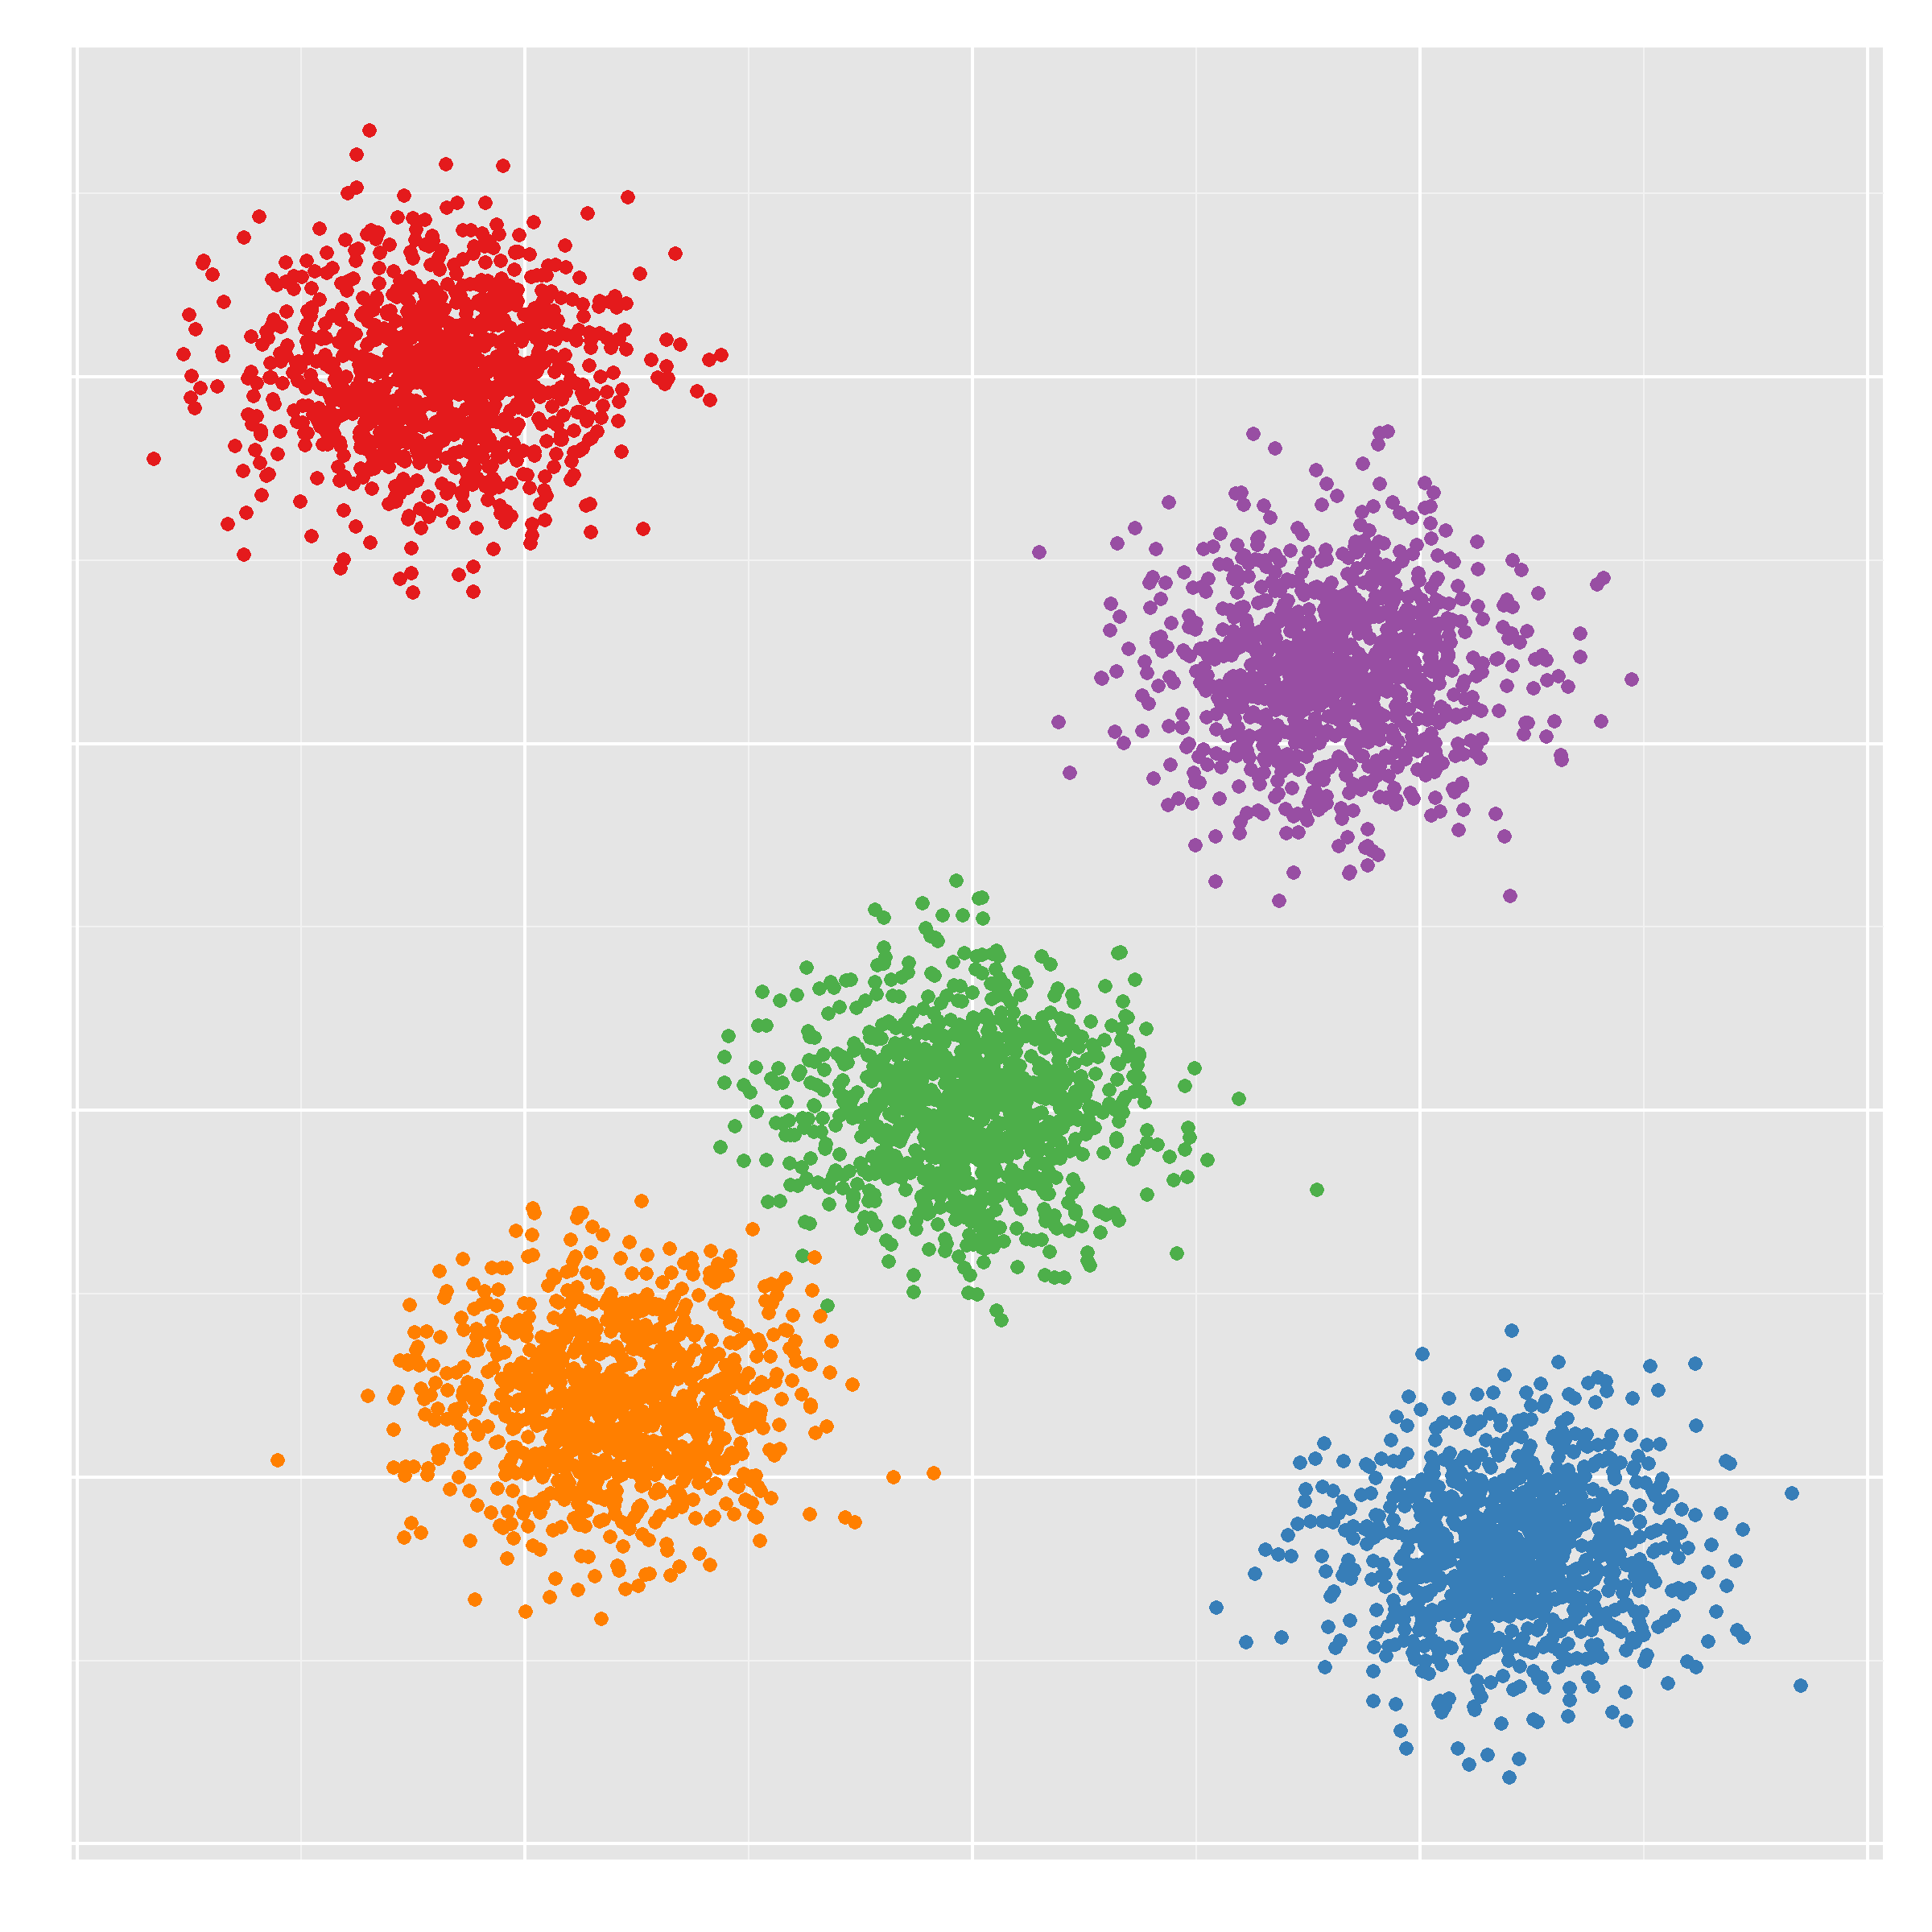
\includegraphics[width = 0.8\textwidth]{my_compact}
    \caption{Convex clusters}
  \label{fig:compact}
  \end{subfigure}
  \begin{subfigure}{0.4\textwidth}
    \centering
    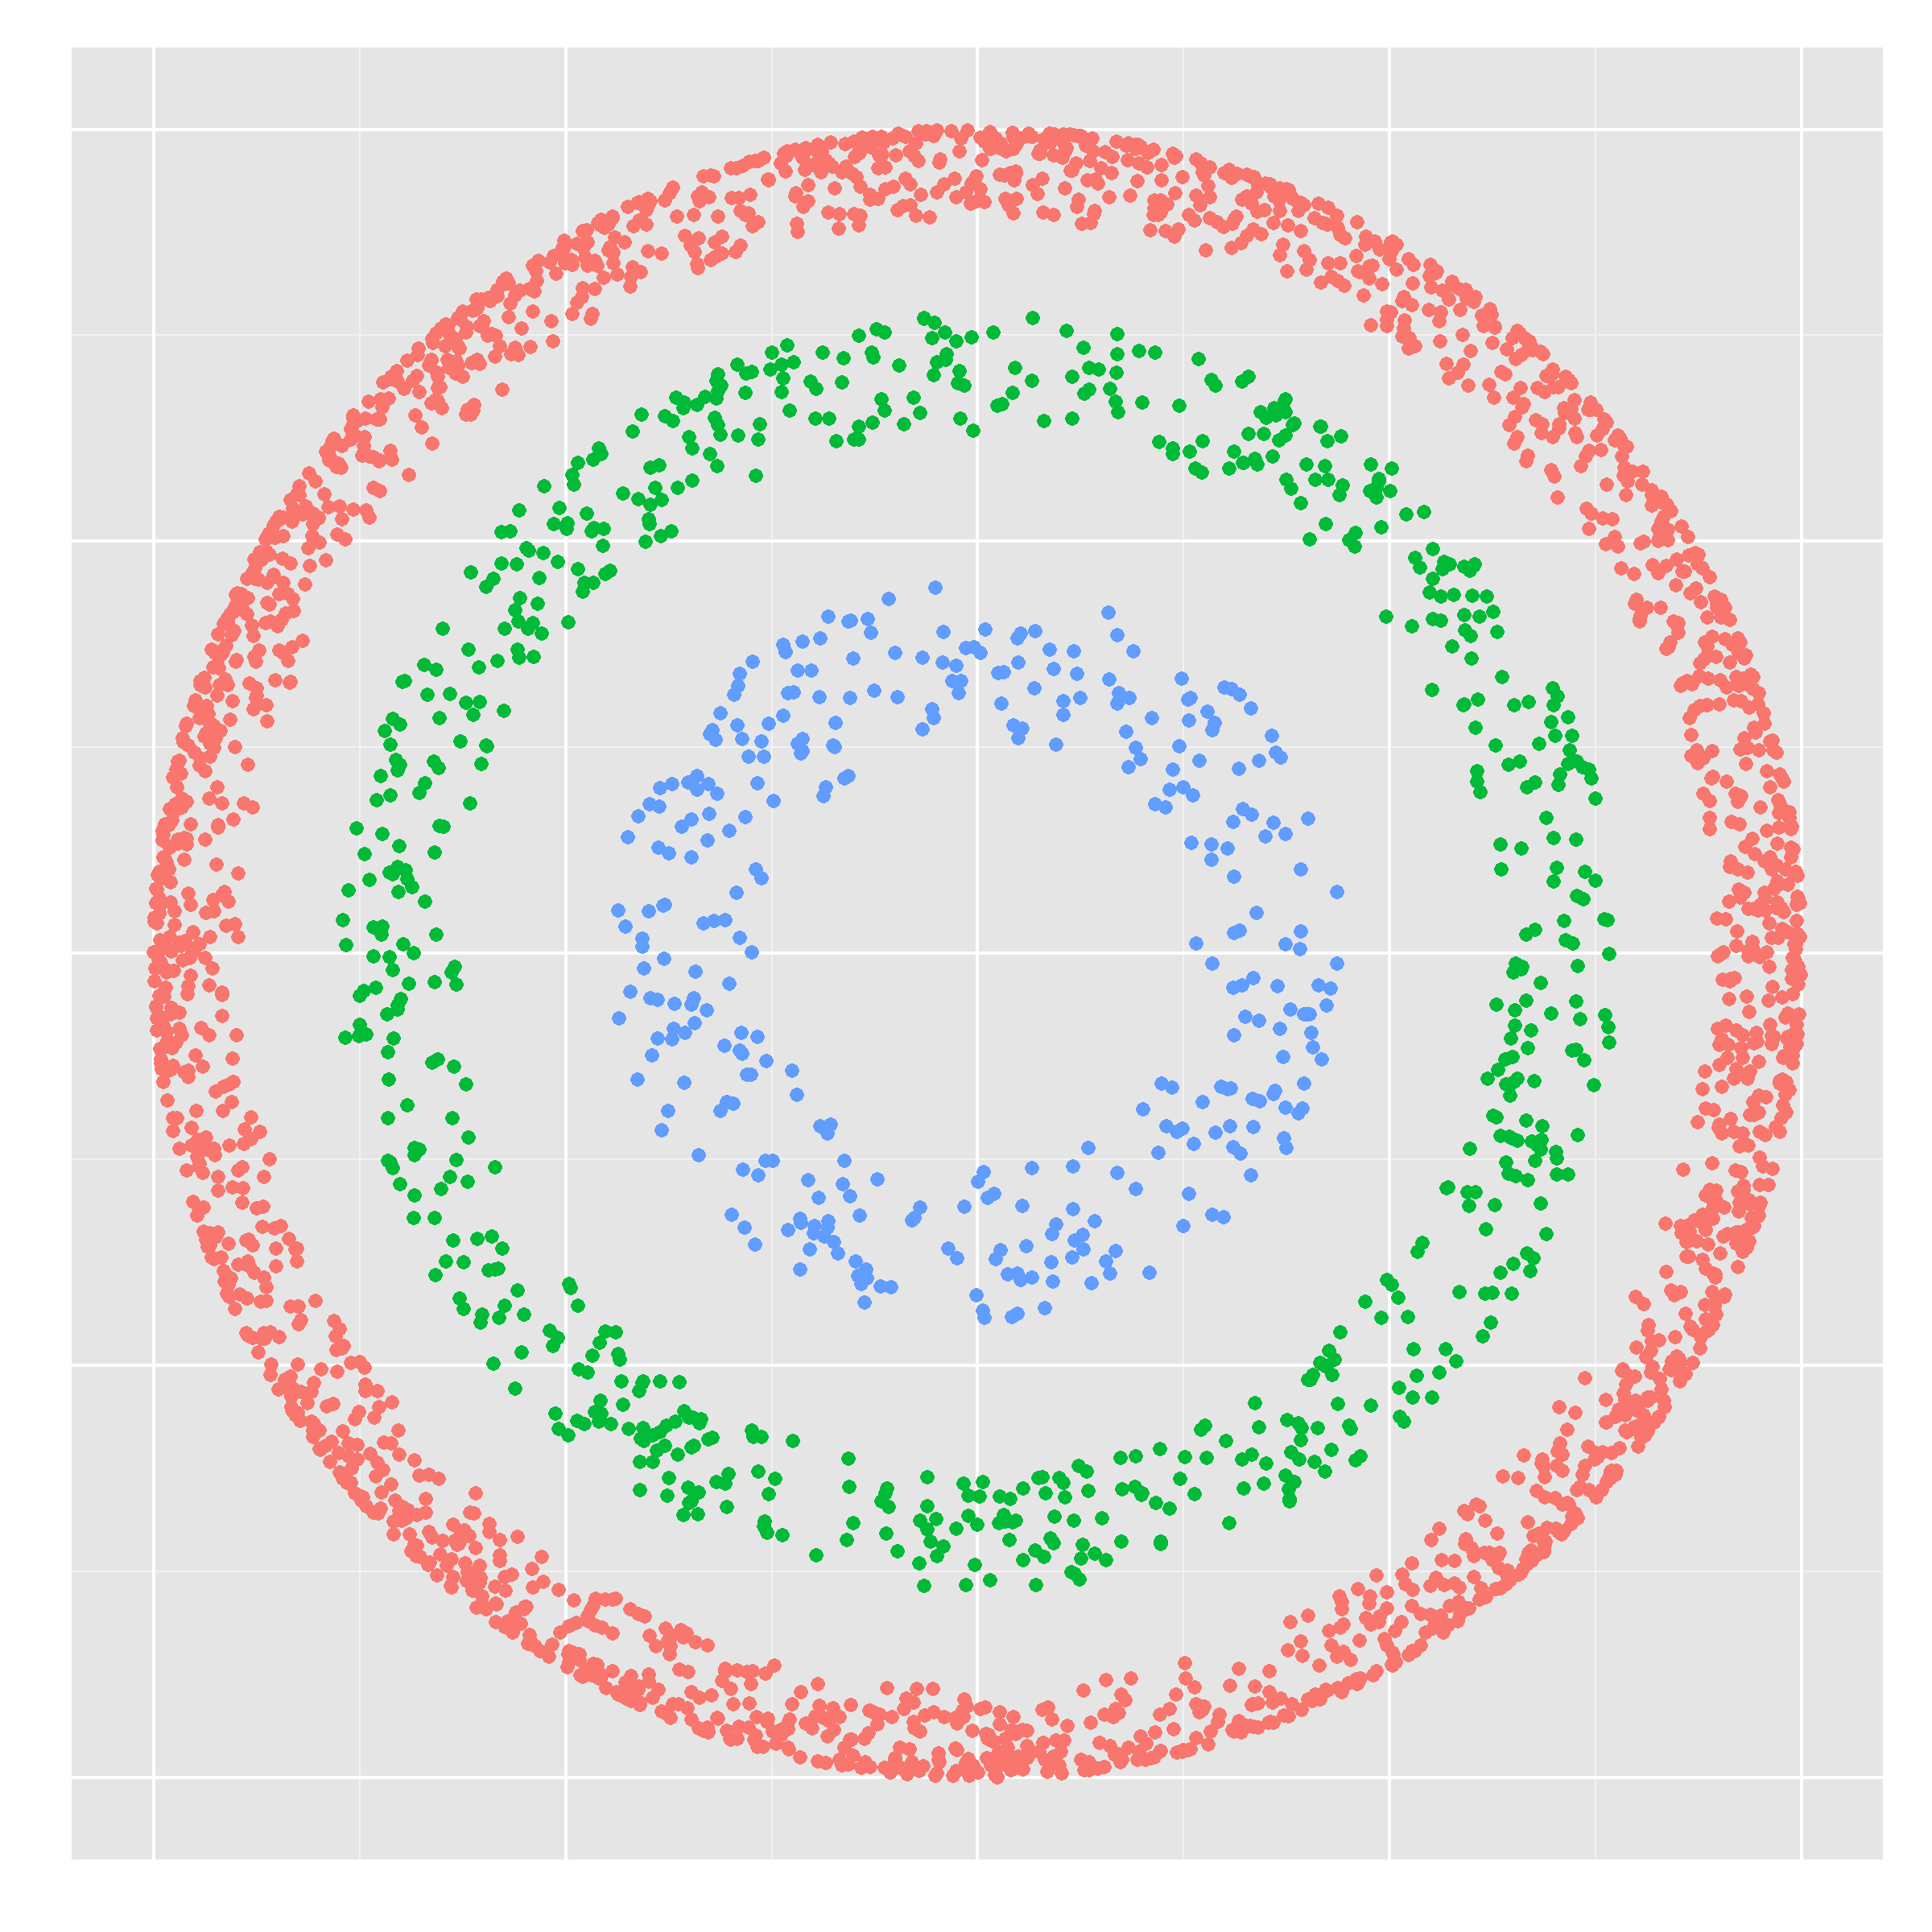
\includegraphics[width = 0.8\textwidth]{my_connected}
     \caption{Non-convex clusters}
     \label{fig:connected}
     \end{subfigure}
  \caption{Examples of different types of clusters}
  \label{fig:compact_connected}
\end{figure}

Simple clustering algorithms such as k-means are good at clustering data in which the underlying true clusters are convex An example of convex clusters is given in Figure \ref{fig:compact}. However k-means can fail when the true clusters are non-convex like those shown in Figure \ref{fig:connected}. This is because k-means is a centroid based clustering algorithm that clusters data based on how similar they are to cluster centroids. Spectral Clustering instead clusters data based on how similar they are to all other data points, which can lead to good quality segmentation on even these difficult cases.  We do not formally address what is meant by similarity here, but will define this fully in Section \ref{sec:affinity}.

 %Data which is convex may be simple to cluster as the gaps between clusters are easy for simple clustering algorithms like k-means to identify. Connected but non-convex data sets can be much more challenging than convex data sets, and can cause some simple clustering algorithms to fail. The reason that centroid based clustering algorithms such as k-means struggle with data sets like that shown in Figure \ref{fig:connected} is that k-means clusters the data based on how similar they are to cluster centroids. Spectral Clustering instead clusters data based on how \textit{similar} they are to all other data points, which can lead to good quality segmentation on even these difficult cases.  We do not formally address what is meant by similarity here, but will define this fully in Section \ref{sec:affinity}.

The similarity between data points can be neatly represented in a graph structure.  We can then restate the clustering problem as a graph partitioning problem where we wish to find a partition of the graph such that the edges between different groups have low weights (which corresponds to data points being dissimilar) and the edges within a group have high weights (the data points are similar).

In order to introduce Spectral Clustering we first introduce some graph notation and discuss graph cut problems. We will then describe the Spectral Clustering algorithm, and discuss in more detail the notion of similarity. 

\subsection{Graph cut problems} 

Data can be represented as a similarity graph, $G = (V,E)$ where each vertex $v_i \in V$ represents a data point $x_i$. The graph will be undirected, by which we mean the edges denote a two-way relationship.  The graph can then be described by an \textit{adjacency matrix}. Adjacency matrices are a way of depicting the graph structure with binary entries denoting which vertexes are connected by edges and which are not. Figure \ref{fig:sim_graphs} depicts two similarity graphs. Their corresponding adjacency matrices are given in equation \eqref{eq:adj_mat}.  A  value of $1$ in cell (2,3) implies that vertexes $v_2$ and $v_3$ are connected by an edge. Note that both of the example adjacency matrices given below are symmetric, which can be expected as we are dealing with undirected graphs.

\begin{figure}[h!]
  \centering
  \begin{subfigure}{0.4\textwidth}
    \centering
    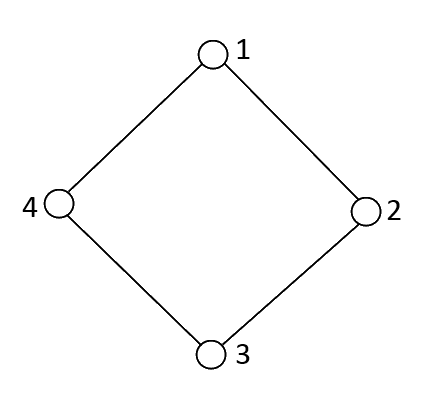
\includegraphics[width = 0.6\textwidth]{adj_square.png}
 %   \caption{cap}
 % \label{fig:adf_square}
  \end{subfigure}
  \begin{subfigure}{0.4\textwidth}
    \centering
    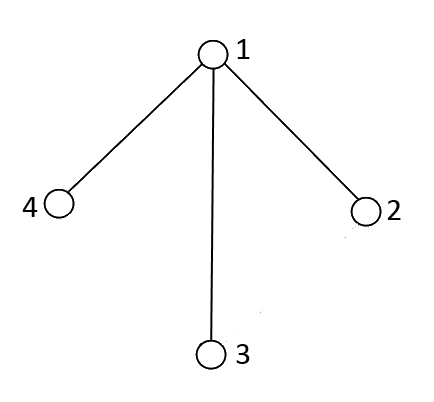
\includegraphics[width = 0.6\textwidth]{adj_tree.png}
%  \caption{Cap}
%  \label{fig:adj_tree}
  \end{subfigure}
  \caption{Two similarity graphs}
  \label{fig:sim_graphs}
\end{figure}

\begin{equation}
\label{eq:adj_mat}
\renewcommand*{\arraystretch}{.5}
  \begin{pmatrix}
    0 & 1 & 0 & 1 \\
    1 & 0 & 1 & 0 \\
    0 & 1 & 0 & 1 \\
    1 & 0 & 1 & 0 
    \end{pmatrix}
\hspace{1.3in}
\renewcommand*{\arraystretch}{.5}
  \begin{pmatrix}
    0 & 1 & 1 & 1 \\
    1 & 0 & 0 & 0 \\
    1 & 0 & 0 & 0 \\
    1 & 0 & 0 & 0 
    \end{pmatrix}
\end{equation}

The \textit{weighted adjacency matrix} (also called an \textit{affinity matrix}) of a similarity graph is the matrix $W = (w_{ij})_{i,j = 1,\ldots, n}$. The weight $w_{ij}$ is the similarity between vertexes $v_i$ and $v_j$.  If $w_{ij}=0$ this means that the vertexes $v_i$ and $v_j$ are not connected by an edge. Again the affinity matrix will be symmetric, that is $w_{ij} = w_{ji}$. 

In order to create a graph partition we need to cut the edges in the graph. Non empty subsets of $V$, $A$ and $B$ will form a partition of the graph $G$ if $A \cap B = \emptyset  $ and $A \cup B = V$.  
The weight of the cut can be calculated by summing the weights of the edges which will be broken when a cut is made. In order to find a good partition of the graph, we wish to choose $A$ and $B$  such that some cut criterion is minimised.  The simplest cut criterion is

\begin{equation}
  \text{cut(A,B)} = \sum_{i \in A, j \in B} w_{ij},\\
  \label{eq:cut}
\end{equation}
where the notation $i \in A$ is short hand to mean the set of indexes $\{ i | v_i \in A \}$.

The Minimum cut \citep{Wu1993} is the cut which minimises equation \eqref{eq:cut}. This can be solved in polynomial time \citep{Stoer1997} however the  minimum cut does not always produce a desirable graph partitioning; it tends to create unbalanced partitions, separating one vertex from the rest of the graph. To understand why this happens, note for a fully connected graph where all verticies are joined by an edge, the number of edges cut in mincut will be  $|A| \times |B|$ which is minimised by the solutions $|A| = 1$ or $|B| = 1$. In order to avoid this, we can specify that the sets $A$ and $B$ are reasonably large in some way. Two common objective functions used to avoid this issue are the RatioCut \citep{Hagen1992} and the normalised cut, Ncut \citep{Malik2000}. 

Both RatioCut and Ncut attempt to normalise the weight of the cut by introducing the size of sets $A$ and $B$. In RatioCut, the size of $A$ is measured by its number of vertexes $|A|$, while in Ncut the size is measured by the weights of its edges $\text{vol}(A) = \sum_{i \in A}d_i$ where $d_i= \sum_{j = 1}^n w_{ij}$ is the \textit{degree} of a vertex $v_i \in V$. The definitions of RatioCut and Ncut are as follows, 

\begin{equation}
  \text{RatioCut(A,B)} = \frac{\text{cut} (A, B)}{|A|} + \frac{\text{cut}(A, B)}{|B|}, 
    \label{eq:ratiocut}
\end{equation}

\begin{equation}
  \text{Ncut(A,B)} = \frac{\text{cut}(A, B)}{\text{vol}(A)} + \frac{\text{cut}(A, B)}{\text{vol}(B)}.
    \label{eq:ncut}
\end{equation}

The main idea in Ncut is that large clusters will increase the denominator vol$(A)$ and thus decrease Ncut$(A,B)$. This will encourage splitting the data into fairly evenly sized clusters, and avoid the minimum cut issue of segmented isolated points. This can be seen in Figure \ref{fig:min_norm_cut}  which depicts both the minimum cut and Ncut solutions for a particular graph. The shaded/non-shaded regions represent the partitioning. The minimum cut isolates one vertex from the rest of the graph, whilst the Ncut provides a more balanced and sensible partition. 

\begin{figure}[H]
  \centering
  \begin{subfigure}{0.4\textwidth}
    \centering
    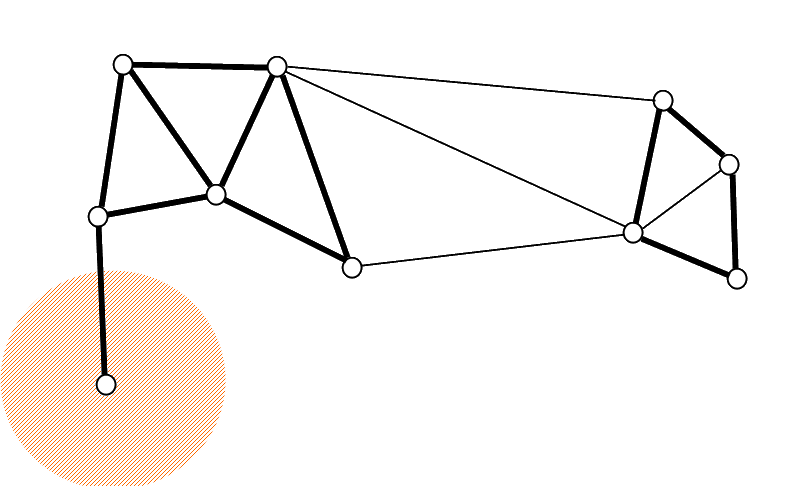
\includegraphics[width = \textwidth]{my_min_cut.png}
    \caption{Minimising the cut.}
  \label{fig:min_cut}
  \end{subfigure}
  \begin{subfigure}{0.4\textwidth}
    \centering
    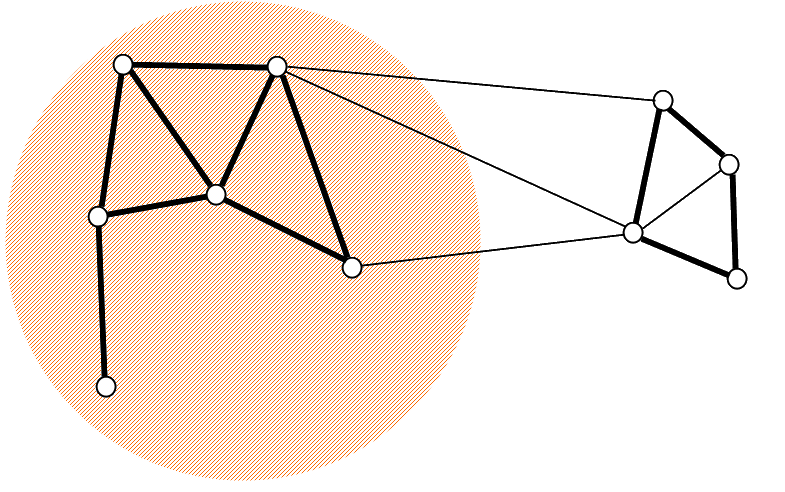
\includegraphics[width = \textwidth]{my_norm_cut.png}
  \caption{Minimising the normalised cut.}
  \label{fig:norm_cut}
  \end{subfigure}
  \caption{Two solutions to the bi-partition problem. The partitioning is indicated by shading/non-shading of nodes.}
  \label{fig:min_norm_cut}
\end{figure}

Although the partitioning has been improved, the previously easy to solve mincut problem (equation \ref{eq:cut}) has been replaced with minimising the normalised cut (equation \ref{eq:ncut}) which is an NP-hard problem \citep{Wagner1993}. Therefore,  a continuous relaxation of the Ncut is solved instead. The solution to the relaxed problem of equation \eqref{eq:ncut} is given by the second eigenvector of the symmetric graph Laplacian defined in equation \eqref{eq:laplacian_symm} \citep{Luxburg2008}. Similarly, the solution of the relaxed problem the ratio cut (equation \ref{eq:ratiocut}) is given by the second eigenvector of the unnormalized Laplacian defined in equation \eqref{eq:laplacian}. Here $W$ is the affinity matrix of the similarity graph and the degree matrix $D$ is defined as the diagonal matrix with the degrees $d_1, \ldots d_n$ on the diagonal. The relaxation of these graph cut problems into the eigen-decompostion of Laplacian matricies is the basis of Spectral Clustering. 
 %It has been shown that the two graph cut optimisations given in equations \eqref{eq:ratiocut} and \eqref{eq:ncut} can be formulated in terms of the spectral decomposition of the graph Laplacian matrices given in equations \eqref{eq:laplacian} and \eqref{eq:laplacian_symm} respectively.  

\begin{eqnarray}
\label{eq:laplacian}
 L =& D - W\\
\label{eq:laplacian_symm}
 L_{\text{symm}} =& D^{-1/2}LD^{-1/2} 
\end{eqnarray}


Unfortunately, there is no guarantee on the quality of the solutions of the relaxed problems compared to the exact solutions \citep{chung1997spectral} and there do exist pathological cases which are arbitrarily bad. However, several papers which investigate the quality of the clustering of Spectral Clustering \citep{Spielman1996, Kannan2004} find Spectral Clustering to provide good solutions. 

The Spectral Clustering algorithm that we use \citep{Ng2001} uses the symmetric Laplacian  $L_{\text{symm}}$. The full Spectral Clustering algorithm is given in Algorithm \ref{alg:njw}. Note that the number of clusters is assumed to be known and this will be the case throughout this chapter.


\begin{algorithm}
\caption{NJW Spectral Clustering algorithm}
\begin{algorithmic}[1]
\REQUIRE Data set $X = \{x_1,\ldots, x_n \}$, number of clusters $k$
\ENSURE $k$-way partition of the input data
\STATE Construct the affinity matrix $W = (w_{ij})_{i,j = 1,\ldots, n}$ %by the following Gaussian kernel function:
%\begin{equation*}
 % w_{i,j} = \exp  \left( - \frac{\| x_i - x_j \|^2}{2 \sigma^2} \right), i,j = 1, \ldots,n.
%\end{equation*}

\STATE Compute the normalised Laplacian matrix  $L_{\text{symm}} = D^{-1/2}( D - W )D^{-1/2}$, where $D$ is the diagonal matrix with $D_{ii}=\sum_{j=1}^{n} w_{ij}.$
\STATE Compute the $k$ eigenvectors of $L_{\text{symm}}$, $v_1, v_2,\ldots , v_k,$ associated with the $k$ smallest eigenvalues, and form the matrix $ V = [v_1,v_2, \ldots ,v_k]$.
\STATE Renormalise each row of $V$ to form a new matrix $Y$.
\STATE Partition the $n$ rows of $Y$ into $k$ clusters using  k-means.
\STATE Assign the original data point $x_i$ to the cluster $l$ if and only if the corresponding row $i$ of the matrix $Y$ is assigned to the cluster $l$.
\end{algorithmic}
\label{alg:njw}
\end{algorithm}

Once the Laplacian has been calculated, one computes the $k$ eigenvectors which correspond to the $k$ smallest eigenvalues of the Laplacian. A matrix $Y \in \mathbb{R}^{n \times k}$ is created, where each column is an eigenvector of the Laplacian, with length $n$. We can view this matrix $Y$ as an embedding of the original data $X$ into a lower dimensional subspace. When represented in this low subspace the clustering problem is often easier, and can be solved with a simple clustering algorithm such as k-means. For example, Figure \ref{fig:spirals_original} shows a data set of three spirals depicted in the original feature space. This is visually quite difficult to cluster. Figure \ref{fig:spirals_embedded} plots the same data set but embedded in the lower dimension, plotting the first eigenvector of the Laplacian against the second eigenvector. Clustering in the embedded space is easy even for k-means to solve. 


\begin{figure}[h!]
  \centering
  \begin{subfigure}{0.4\textwidth}
    \centering
    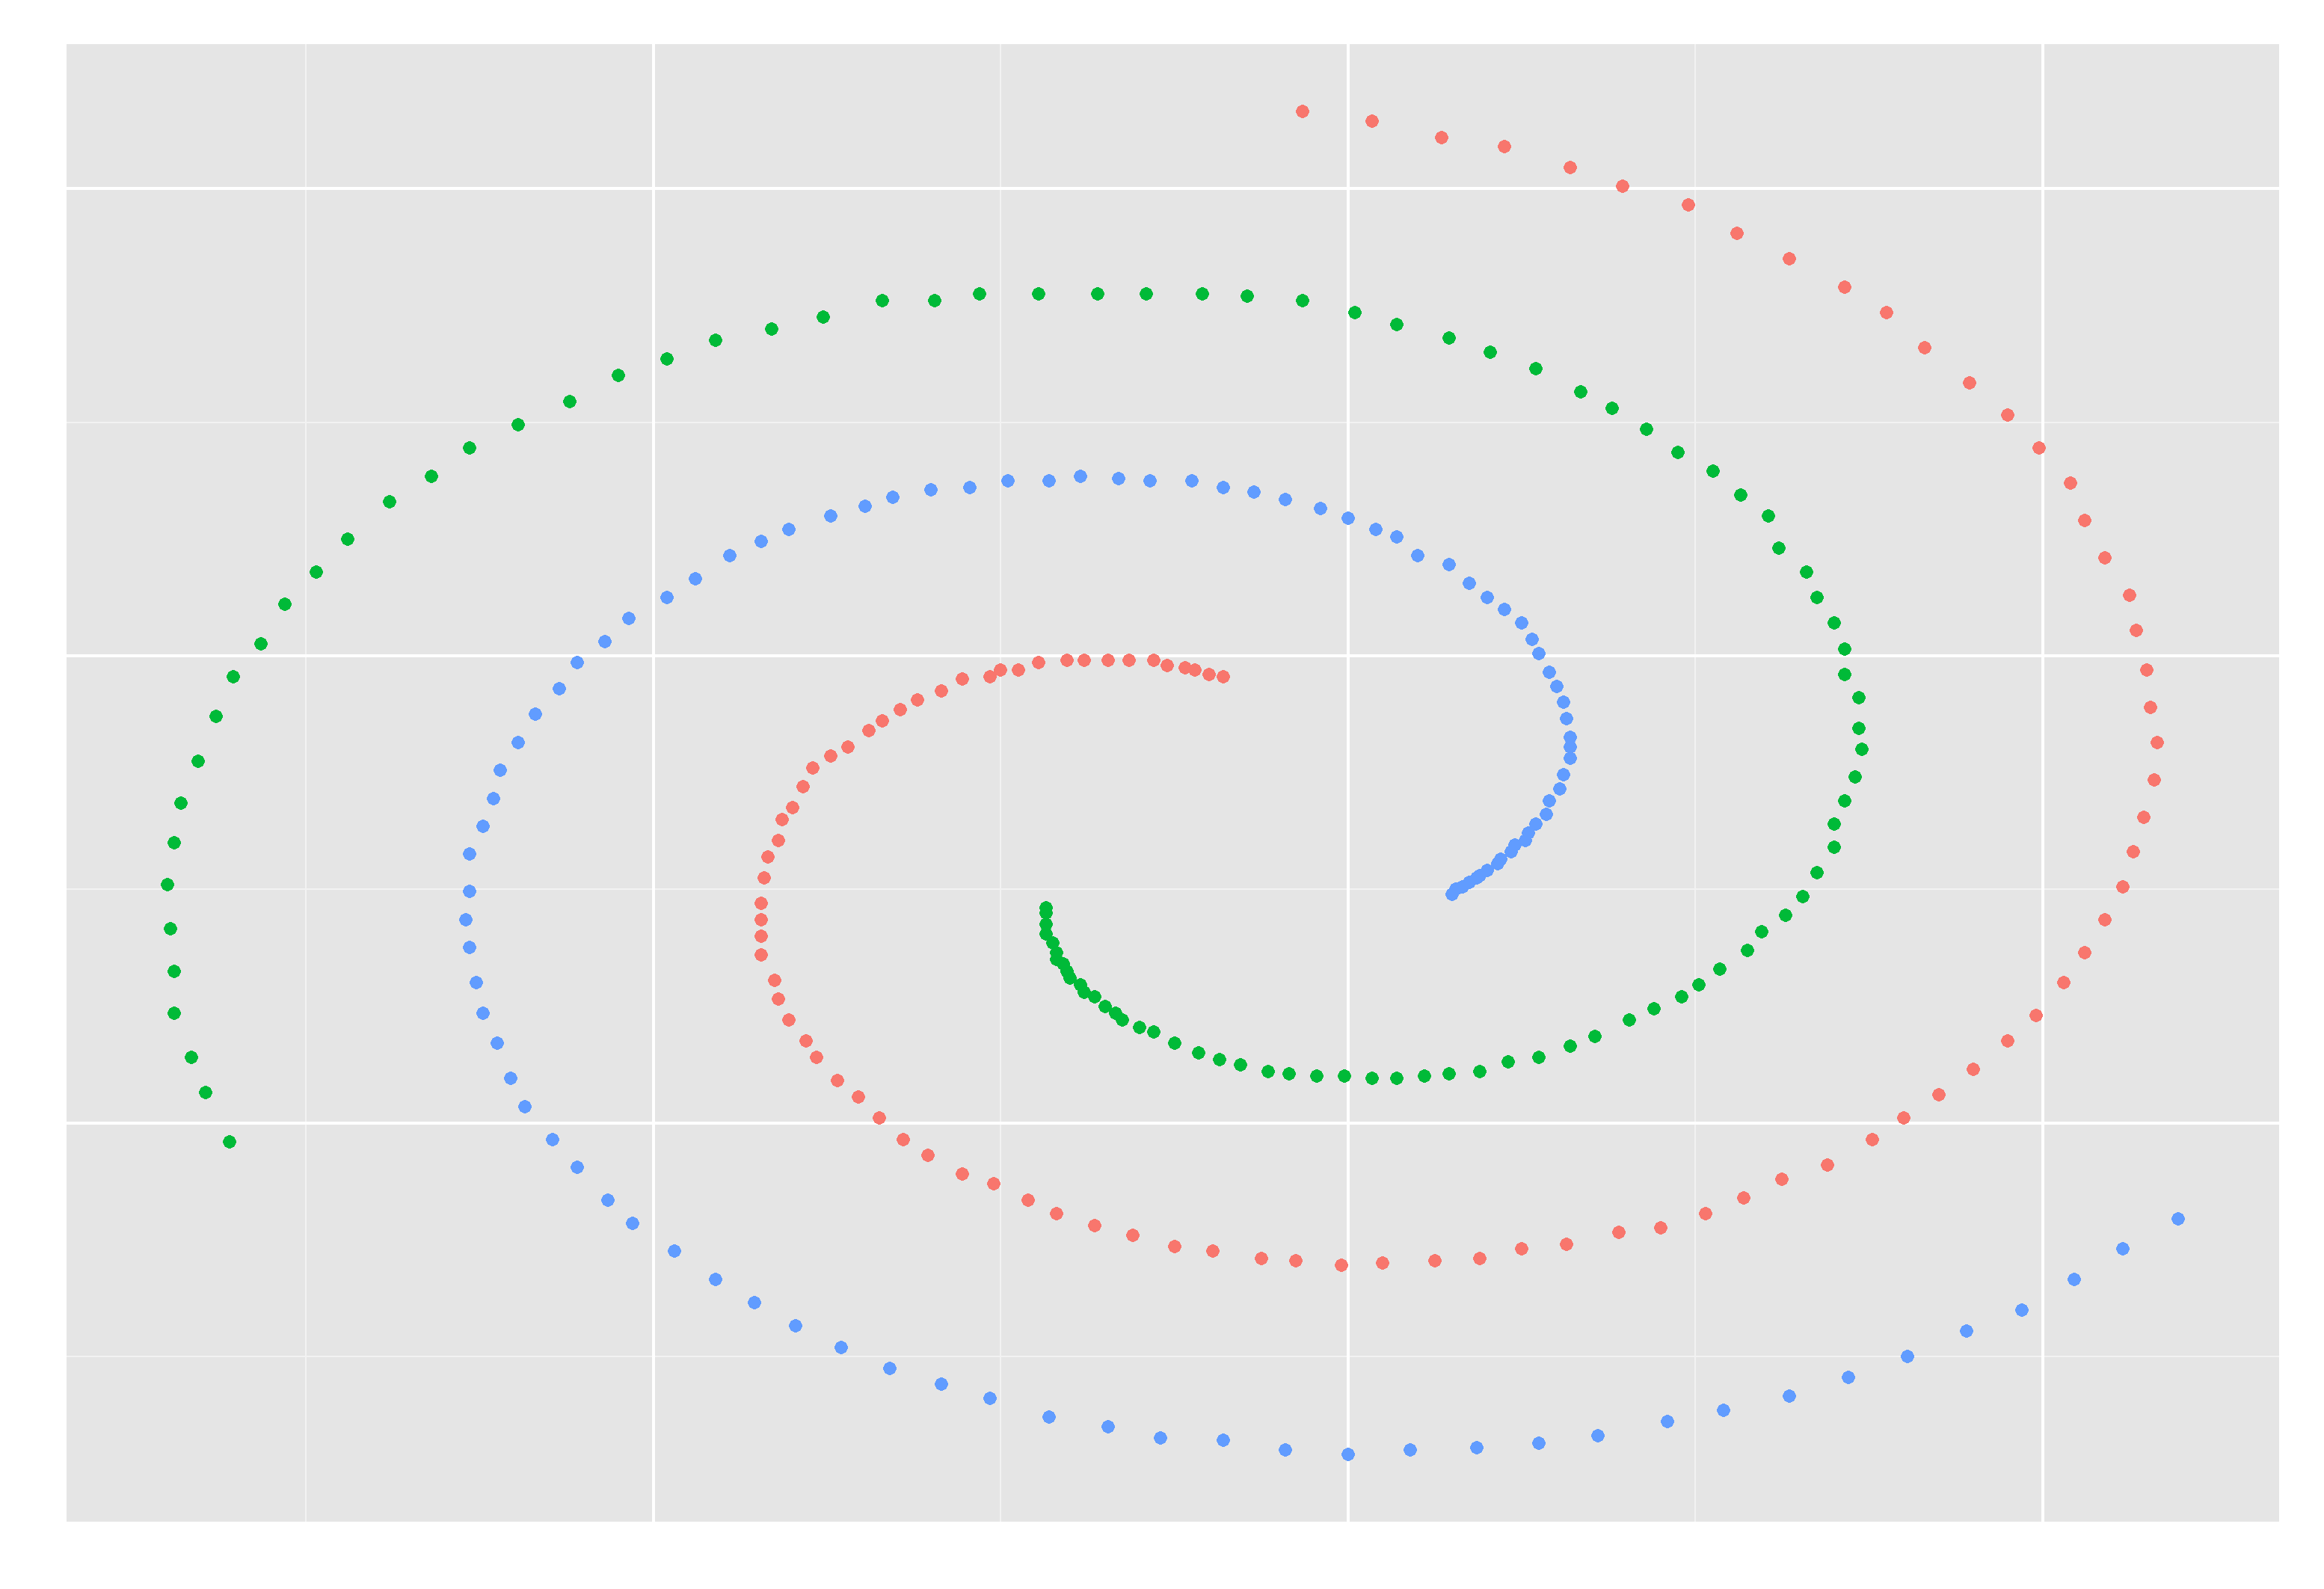
\includegraphics[width = \textwidth, height = \textwidth]{code_embedding/3_spiral_original.png}
    \caption{Data viewed in the original \\ feature space}
  \label{fig:spirals_original}
  \end{subfigure}
  \begin{subfigure}{0.4\textwidth}
    \centering
    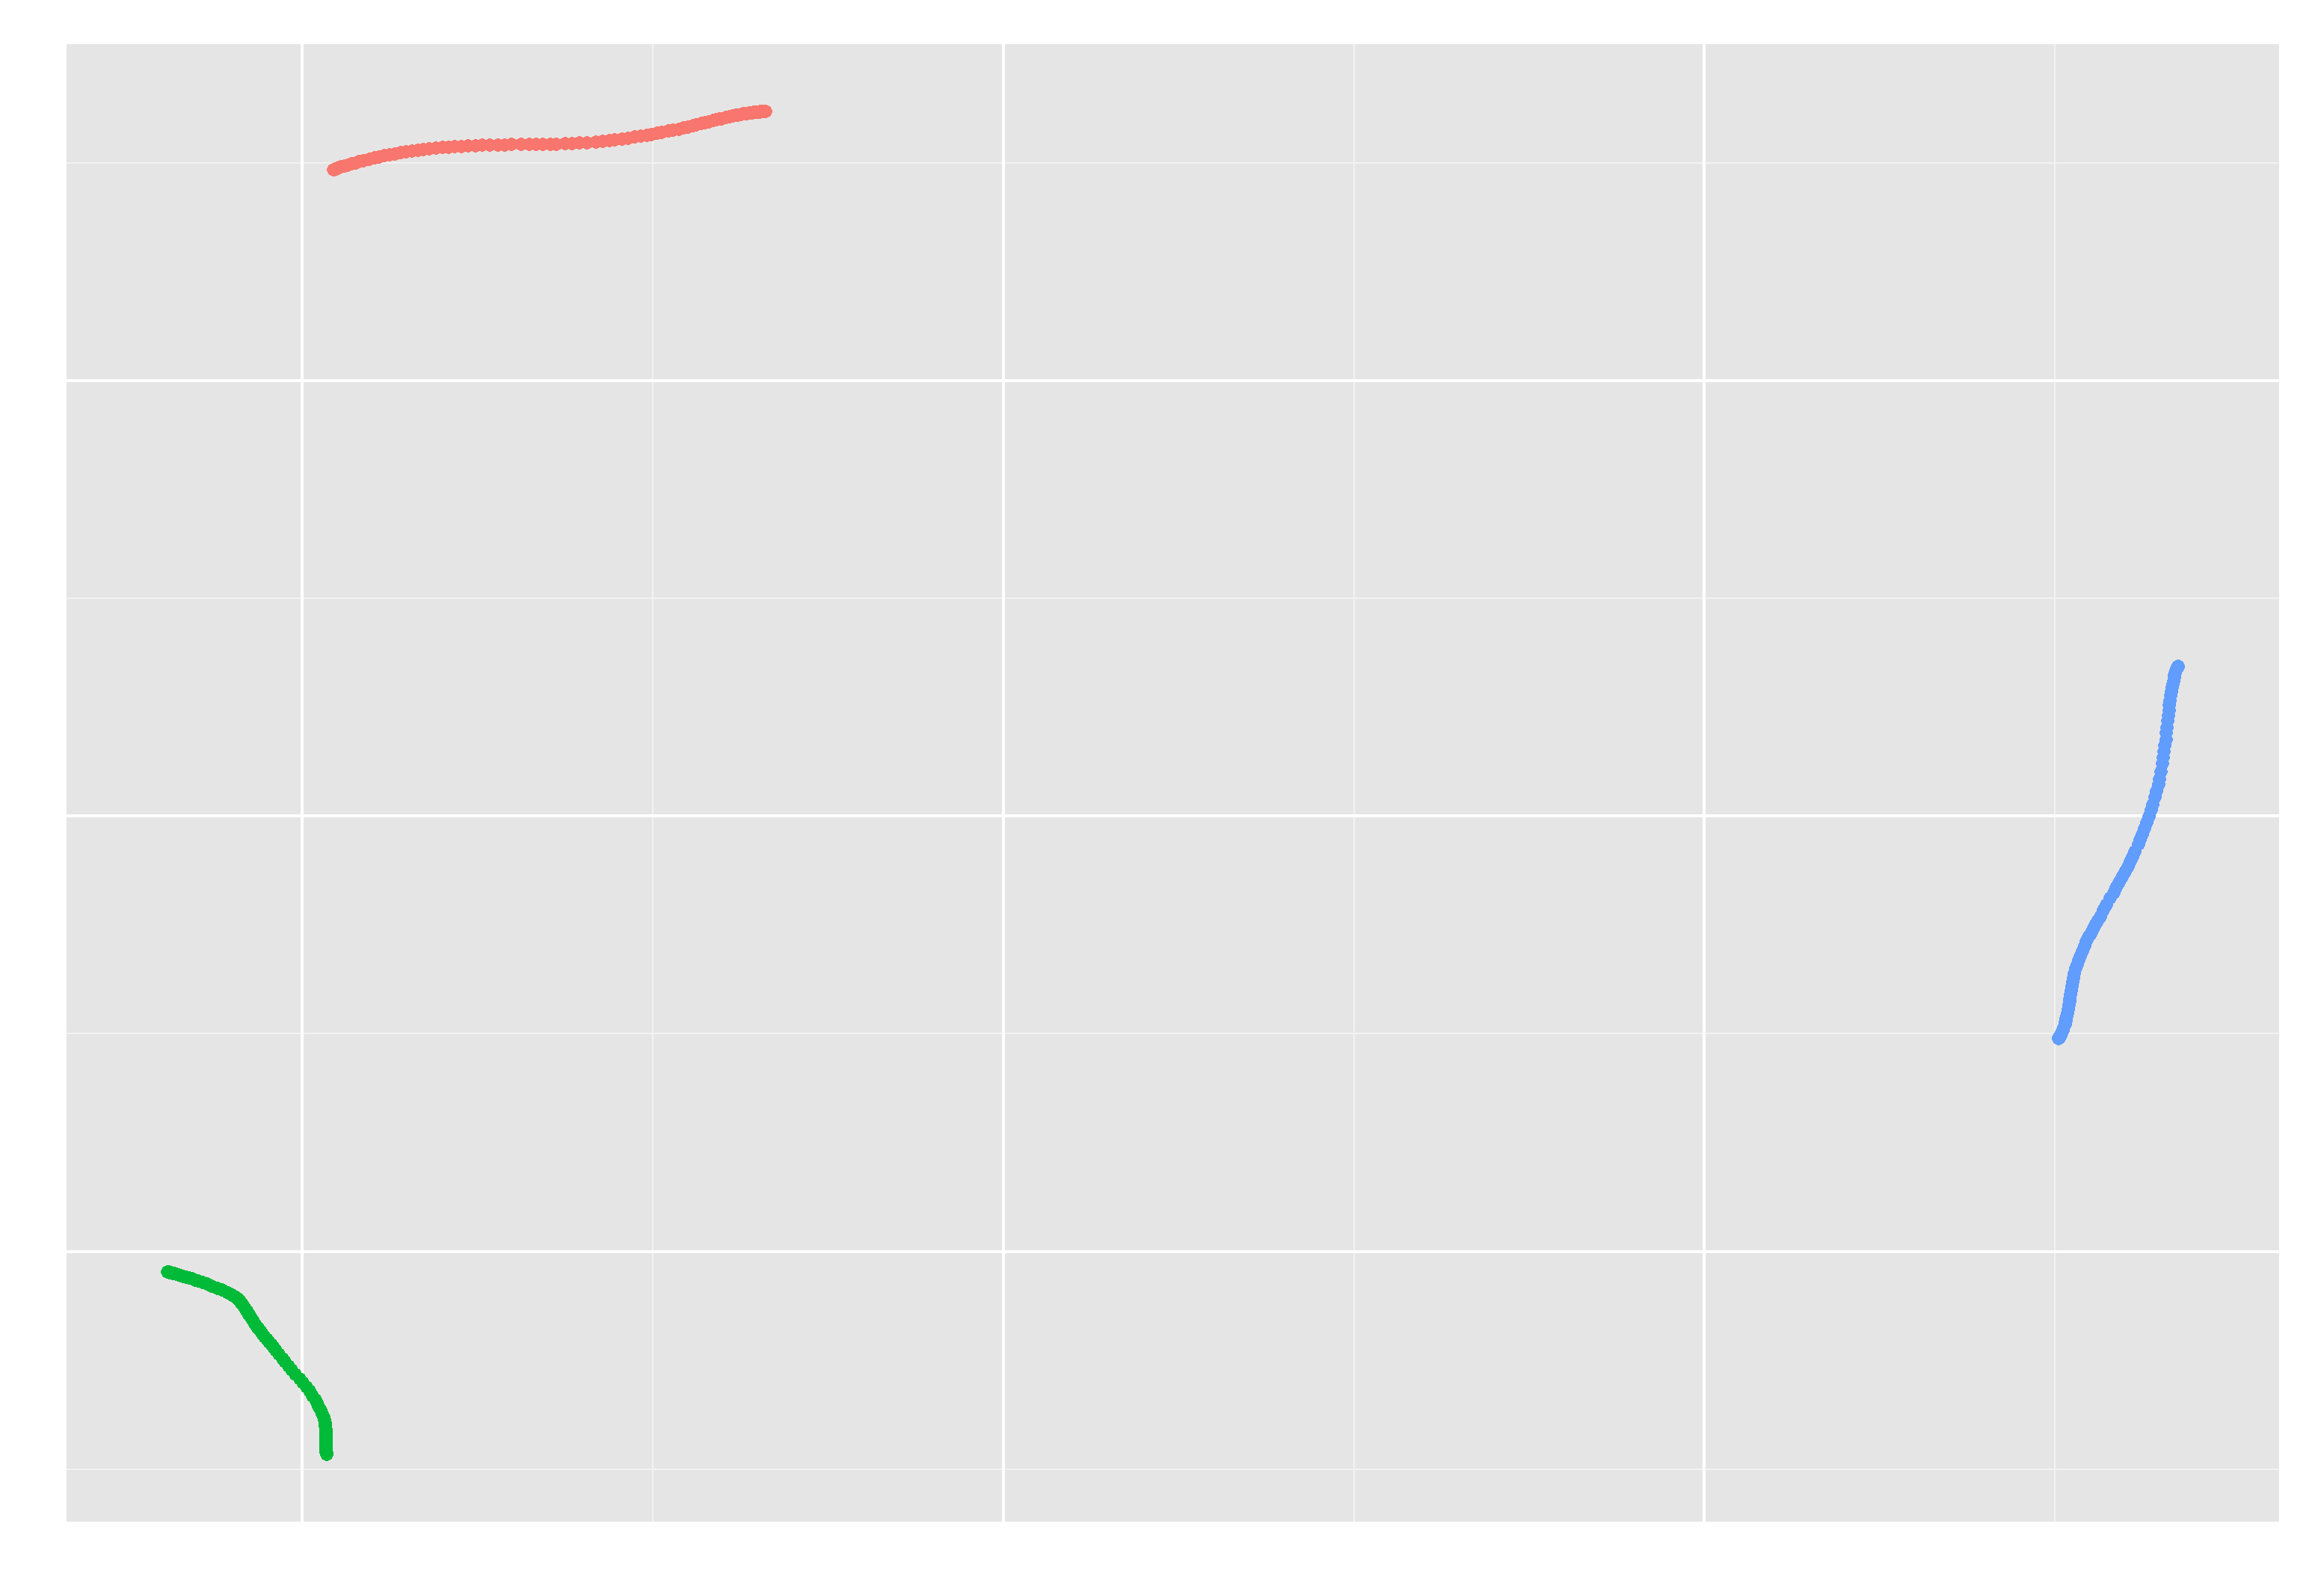
\includegraphics[width =\textwidth, height = \textwidth]{code_embedding/3_spiral_embedded.png}
     \caption{Data viewed in the 2-dimensional \\ embedding space }
     \label{fig:spirals_embedded}
     \end{subfigure}
  \caption{Triple spiral data set viewed in feature space and eigenvector embedding}
  \label{fig:triple_spirals}
\end{figure}


After the embedding, k-means can be used to cluster the $n$ rows of $Y$ into $k$ clusters. Finally, assign the cluster label given to each row $Y_i$ to the corresponding original data point $x_i$. Now that we have introduced the general Spectral Clustering algorithm, we will discuss the notion of similarity in more detail.

\subsection{Choice of affinity matrix}
\label{sec:affinity}

One of the key factors of Spectral Clustering is the affinity matrix $W = (w_{ij})_{ i,j = 1, \ldots, n}$  which represents the pairwise similarities between all data points $x_i$ and $x_j$. A popular choice is to use the Gaussian kernel, 

\begin{equation}
  \label{eq:gaussian_affinity}
    w_{i,j} = \exp  \left( - \frac{\| x_i - x_j \|^2}{2 \sigma^2} \right), \; i, j = 1, \ldots, n,
\end{equation}
where the parameter $\sigma$ controls the width of the local neighbourhoods which we want to model. If $x_i$ and $x_j$ are very close, then $w_{ij} \rightarrow 1 $, and if they are far apart $w_{ij} \rightarrow 0$. A Gaussian kernel affinity matrix will have ones along the diagonal and is symmetric $(w_{ij} = w_{ji})$.

The scaling parameter $\sigma$ is usually chosen manually. \cite{Ng2001} automatically choose $\sigma$ by running their clustering algorithm repeatedly for a number of values of $\sigma$. They then select the $\sigma$ which provides least distorted k-means clusters in step 5 of Algorithm \ref{alg:njw}. \cite{Zelnik-Manor2004} argue that for data which has a cluttered background, or multi-scale data, one global parameter choice for $\sigma$ is not sufficient. They calculate a localised parameter $\sigma_i$ for each data point $x_i$ based on its neighbourhood. Using a localised $\sigma_i$ can deal well with multi-scale data, but requires the user to choose the size of the neighbourhood in order to calculate $\sigma_i$. 

If we mainly wish to model the local relationships then using all of the possible pairwise data similarities may not be necessary. It is possible to use a weighted k-nearest neighbour structure \citep{Luxburg2008} to build the affinity matrix once corrections have been made to ensure that this matrix is symmetric. Another option is to choose some threshold $\epsilon$ and only consider connections between data points whose pairwise similarities are greater  than some threshold $\epsilon$. This is an $\epsilon$-neighbourhood graph as shown in equation \eqref{eq:epsilon_graph}. 

%Although it is possible to weight this graph by $\epsilon$, if we choose $\epsilon$ to generate a small $\epsilon$-neighbourhood, then the differences between the weights will be so small that weighting may become eligible.

\begin{equation}
\label{eq:epsilon_graph}
  w^*_{ij}=\left\{
  \begin{array}{@{}ll@{}}
    1, & \text{if}\ w_{ij} > \epsilon \\
    0, & \text{otherwise}
  \end{array}\right.
\end{equation} 

Using this construction will give a sparse affinity matrix instead of a fully connected graph, which will help lower the computational complexity. 

\section{Advanced Spectral Clustering}
\label{sec:ad_spec}

In the previous section we introduced Spectral Clustering via graph partitioning and discussed options for creating affinity matrices. Our overall aim is to perform Spectral Clustering on data streams. First, we consider some of the challenges that make clustering in data streams so difficult, and look at the approaches that exist to deal with these challenges in the Spectral Clustering setting.

 The first challenge that is addressed is dealing with big data. One of the main difficulties in data streaming is the pure volume of data available and the methods discussed in Section \ref{sec:big_data} offer methods to perform Spectral Clustering on big data.  Another difficulty that arises in data streaming is the ability to update the current clustering result  as new data arrives.  This problem is called Incremental Spectral Clustering and is discussed in Section \ref{sec:incremental}.

It is stressed that these problems (large data and incremental data) are just sub-problems of what makes data streaming difficult, and therefore none of the methods described below are capable of dealing with the full data streaming problem. The solutions offered to speed up computation for large data sets cannot update the clustering result if a new data point arrives. The incremental spectral clustering algorithms can update cluster membership as new data arrives but do not scale as for very large or possibly infinite $n$. %The even more challenging setting of data streams, will be addressed in Section \ref{sec:microSpec}.    

\subsection{Large-scale Spectral Clustering}
\label{sec:big_data}

%Although Spectral Clustering has been shown to perform well empirically on simple data sets, computational problems arise as the data set size increases.  
Spectral Clustering can be challenging for very large data sets since constructing the affinity matrix $W$ and computing the eigenvectors of $L$ have computational complexity $\mathcal{O}(n^2)$ and $\mathcal{O}(n^3)$ respectively. The Nystr\"{o}m method \citep{Williams2001} is a general method for generating good quality low rank approximations of large matrices. The Nystr\"{o}m approximation method for Spectral Clustering \citep{Fowlkes2004} randomly samples the columns of the affinity matrix $W$ and approximates the eigen decomposition of the full matrix directly using correlations between the sampled columns and the remaining columns. Effectively this can be thought of as a dial which the user has control over, sampling more columns will provide better results but at a higher computational cost. The downsides with this method are that the  memory requirements can be high and the random sampling of columns may lead to small clusters being under represented or completely missed in the final clustering. 
%Doesn't use the affinity to choose which columns in the matrix to sample.
%Fixed complexity dependant on the number of verticies $n$ and the number of samples columns $q$
%DRINEAS/MAHONEY non-uniform sampling of the Gram matrix and bounds approximation error
%But may need to sample many columns (O(n)?)
%practicaltiy on massive datasets may be limited according to Yan. (how big is massive?)
%DRINEAS/MAHONEY non-uniform sampling of the Gram matrix and bounds approximation error
%But may need to sample many columns (O(n)?)

% Spectral Clustering is performed on the representative set only, which is significantly faster than performing Spectral Clustering on the full data set. The resulting cluster labels for the representative data are linked back to the original data set such that every original data point acquires the same label as its associated $k$-means cluster centre. 

An alternative to the Nystr\"{o}m method is to use a pre-processing technique to reduce the size of the data. A natural way to do this is to select certain representative points to summarise the whole data set.  \cite{Yan2009} proposed KASP and RASP, algorithms which use k-means and random forest methods respectively to select $q$ representative points to apply Spectral Clustering on.  Similarly \cite{Shinnou2008} also use $k$-means to identify representative points, but in addition to using these points, \cite{Shinnou2008} also include any data points which are deemed to be suitably far from any representative point in the Spectral Clustering.  In both \cite{Yan2009} and \cite{Shinnou2008} the cluster labels given to the original data points are the same as the label assigned to their nearest representative point. As an alternative, \cite{Chen2011} represents the data as a linear combination of representative points. Random sampling has been applied to reduce the size of the data points within the eigen-decomposition step. \cite{Chen2006a, Liu2007} introduce early stopping strategies to speed up eigen-decomposition based on the observation that well-separated data points will converge more quickly to the final embedding. However this is only suitable for binary clustering.  Other possibilities include random projection with sampling methods \citep{Sakai2009} and shortest path methods \citep{Liu2013b}.

%\cite{Chen2011} has a ``landmark `` based SC.  $q$ landmark points are chosen to represent the data (randomly or with k-means), and the rest of the data is represented as a linear combination in a codebook type formar. % $\mathcal{O}(nq)$ and $\mathcal{O}(q^3 + q^2n)$. 

We discuss the KASP algorithm in more detail as it is the most popular speed up method for Spectral Clustering and it inspired our work in online Spectral Clustering which is introduced in Section \ref{sec:microSpec}.

In KASP, k-means is applied with $q$ clusters to the data set $X$, where $q$ is chosen such that $k \ll q \ll n$. Therefore each point in $X$ belongs to a cluster $y_j, (j \in 1, \hdots, q)$. Let the centres of these $q$ clusters be  $\widehat{y_1}, \hdots, \widehat{y_q}$. These  are used as representative points for the whole data set. Spectral Clustering is performed on the representative points, reducing the complexity of the eigen decomposition from $\mathcal{O}(n^3)$ to $\mathcal{O}(q^3)$. Finally, the original data points are assigned the cluster label  that their closest representative point $\widehat{y_j}$ was assigned in the Spectral Clustering. The KASP algorithm is given in Algorithm \ref{alg:kasp}.

\begin{algorithm}[h!]
\caption{KASP}
  \begin{algorithmic}[1]
   \REQUIRE Data set $X = {x_1,\ldots, x_n}$, number of clusters $k$, number of representative points $q$
   \ENSURE  $k$-way partition of the input data
   \STATE Perform k-means with $q$ clusters on $x_1, \hdots, x_n$ to create clusters $y_1, \hdots y_q$.
   \STATE Compute the cluster centroids $\widehat{y_1}, \hdots, \widehat{y_q}$ as the $q$ representative points.
   \STATE Build a correspondence table to associate each $x_i$ with the nearest cluster centroids $\widehat{y_j}$.
   \STATE Run a Spectral Clustering algorithm on $\widehat{y_1}, \hdots, \widehat{y_q}$ to obtain an $k$-way cluster membership
   for each of $\widehat{y_j}, (j \in 1 \hdots q)$.
   \STATE Recover the cluster membership for each $x_i$ by looking up the cluster membership of the corresponding centroid $\widehat{y_j}$ in the correspondence table.
  \end{algorithmic}
\label{alg:kasp}
\end{algorithm}

Both KASP and RASP have been shown to perform well empirically on large data sets \citep{Yan2009}, retaining good clustering performance even as the \textit{data reduction ratio} increases. We can express the data reduction ratio as $\gamma = \frac{n}{q}$. As in many of the sampling methods discussed above, in KASP the user has control over the data reduction rate. A larger value of $q$ will give a better performance but at a computational cost. The KASP authors present an upper bound on the misclustering rate given the perturbation to the original data. This bound tells us how different the clustering output is if we use the full data set to cluster compared with if we just use the representative points. However, there are a number of assumptions required \citep{Huang2008} relating to the ability for the data to be separated into clusters. Also, this bound does not inform us about the quality of the clustering generally, only as a comparison to clustering the full data set. Finally, the method of assigning data points to clusters based on the cluster label of their representative point can lead to poor segmentation as shown in \cite{Cao2014}. They propose a local interpolation in their algorithm Local Information-based Fast Approximate Spectral Clustering (Li-ASP) to prevent this poor segmentation issue. They achieve this by assigning data points based on a weighted version of their $p$ closest representative points labels, rather than labelling based just on the label of the single closest representative point. 
 
% One constant challenge in clustering is selecting the number of clusters to search for. \cite{Zelnik-Manor2004} present a method for automatically choosing the true number of clusters using the eigenvectors to inform their choice. More commonly the eigenvalues are used to estimate the number of clusters, but if the clusters are not clearly separated identifying the number of clusters from eigenvalues alone is not trivial. We shall assume that the true number of clusters is known. 

The methods discussed above only address dealing with large data sets which are static. Our aim is to investigate methods which can update the Spectral Clustering partitioning when new data points arrive. 

\subsection{Incremental methods for Spectral Clustering}
 \label{sec:incremental}

Incremental Spectral Clustering methods are spectral clustering algorithms which are able to update their cluster partitioning when a new data point or batch of data point arrives. The term incremental is used here rather than online because although these algorithms can update when new data points arrive, they are not designed to deal with the full data streaming scenario. As a reminder, data streams are defined by the constant arrival of data points at a high velocity relative to the available processing power. On the other hand, Incremental Spectral Clustering algorithms are designed for the problem of an evolving network.

For example, lets say we are interested in understanding academic relationships within Lancaster University. We may first define a similarity score between two academics based on the number of papers that they have authored together. We could then use this similarity to create an affinity matrix and perform spectral clustering to discover the academic clustering within the University.  However this affinity matrix will not remain static. A new academic may join the University, or two existing academics may author a new paper changing their similarity score. Performing a full re-clustering of the whole University may be costly and potentially not computationally feasible. Instead, we may wish to update our clustering solution just by incorporating this new information. This is the type of problem that Incremental Spectral Clustering algorithms seek to address.  So far there have been two different approaches to this problem (i) updating the cluster membership directly (ii) incrementally updating the eigenvectors.

%A data stream is a potentially endless sequence of observations obtained at high frequency relative to the available processing and storage capabilities. Data streams arise in many applications such as online purchases, modelling epidemics and understanding sensor networks. %A data stream is a potentially endless sequence of observations obtained at high frequency relative to the available processing and storage capabilities. Data streams arise in many applications such as online purchases, modelling epidemics and understanding sensor networks. 


The first method is described in \cite{Valgren2008}. When new points arrive, the Spectral Clustering is updated directly using a similarity threshold to assign points to clusters. If a new data point is sufficiently far from its closest representative points, it is considered the start of a new cluster. This means that the number of overall clusters  must always increase. Therefore it is not feasible for data streams. In addition there is no method for splitting existing clusters as new data points arrive. %i There are a number of problems with this method. The number of clusters (and therefore the size of the affinity matrix) must always increase. Can't deal with cluster splits. %Affinity is shrunk whenever new cluster is added.

An algorithm that incrementally updates the eigenvectors is proposed in \cite{Ning2007} and  \cite{Ning2010}. Their algorithm can deal with both additional data points joining the network and similarity weights changing between existing data points. The algorithm updates the eigenvectors and eigenvalues directly without performing a full eigen-decomposition. The addition of a new data point is treated as a series of $n$ weight changes, where is $n$ is the number of currently observed data points.  However the authors recommend a full re-clustering in batch to minimise cumulative errors. There are some issues with their update method, mainly that the updating of eigenvectors means that the orthogonality property may be lost - potentially leading to poor cluster detection. Also if the spatial neighbourhoods of often changing vertexes are large it can still be computationally difficult as the eigenvector update step involves the inversion of a matrix. Finally the authors recommend a full spectral re-clustering occasionally to prevent the accumulation of errors in the eigenvectors, this is not feasible in the streaming setting. Generally this method is not suitable for data streaming, as the size of the Laplacian can grown unbounded for an infinite data stream. Another incremental update algorithm is detailed in \cite{Dhanjal2014} which approximates the eigen decomposition of the Laplacian incrementally but still requires regular full re-clustering. %\cite{Dhanjal2011} %We did intend to use this algorithm as a competing algorithm in our experiments section. However, the computational costs for Ning were so great for data streaming examples that it was not possible to run the study, even when not performing a full reclustering.

\cite{Kong2011} is a mixture of both Ning and Valgren's methods, using representative points like Valgren but the eigen-updating of Ning. Although it can be quicker that Ning it retains the other issues of Ning's method discussed above. In addition it has the same problem of Valgren's method that the number of clusters increases over time. This makes it unsuitable for data streams. %nh in It  It assumes sparse data set. Number of representative points will grow unbounded making it unsuitable for data streams. 

%Other variants include using fuzzy C k-means \citep{Bouchachia2012} and a model based kernel Spectral Clustering \citep{Langone2014}.

Although the methods discussed deal with some aspects of difficulties in data streams, none of them are suitable for the full problem of clustering a data stream. We introduce an online Spectral Clustering algorithm for data streams based on the Clustream model of \cite{Aggarwal2003} in Section \ref{sec:microSpec}.


\section{Clustream for Spectral Clustering}
\label{sec:microSpec}
 
Clustream \citep{Aggarwal2003} is a framework for clustering data streams which separates the clustering process in two stages, a micro-clustering stage and a macro-clustering stage. The  micro-clustering stage continuously updates statistical summaries of the data stream, and the macro-clustering is more computationally intensive and run in batch or on a user request. Clustream has proved popular; since the paper was first published in 2003 it has been cited over 1400 times. In the next subsection we detail how the micro-clustering step in the Clustream algorithm works as described in \cite{Aggarwal2003}. %the concept of micro-clusters. Micro-clusters are data summaries which which allows quick and easy updates and the ability to perform sophisticated clustering algorithms The main idea is to 

\subsubsection{Micro-clustering}

The micro-clustering stage is a way of maintaining an active, evolving representative summary of the data, without storing the absolute values of the data points. Micro-clusters are defined as a temporal extension of the cluster feature vector first described in \cite{Zhang1996a}.% The data stream is summarised by many small clusters, which are initially generated by k-means. The online phase stores $q$ micro-clusters in memory, where $q$ is an input parameter.
We take an initial training set and perform k-means with $q$ clusters but choose the value of $q$ to be much larger than the expected number of true macro-clusters $k$. The aim is to create a fine scale summary of the data. The value of $q$ should be chosen to be as large as computationally comfortable. The larger $q$ is, the finer scale that the summaries will be. It is vital to ensure that the micro-clusters well represent the underlying data set or else the macro-clustering will under perform. These $q$ clusters are our first micro-clusters. Over time, we will update these micro-clusters, adding new data points to them, merging them and removing old micro-clusters, although the number of micro-clusters should stay fixed throughout. 

The micro-clusters can then be used on a user request to perform a macro-clustering using the summarised data rather than the full data set. If the micro-clusters represent the true underlying data stream well, then the difference between the clustering on the summarised data and the true full data should be small. However unfortunately this is not guaranteed by the method.

Assume that we have a data stream $S$ which consists of $d$-dimensional data $\boldsymbol{x_i}$ arriving in sequence, $S = \{\boldsymbol{x_i} \}_{i \in \mathbb{N}}, \boldsymbol{x_i} \in \mathbb{R}^d$. Each micro-cluster $M_j, (j \in 1 \ldots, q)$ is stored as a ($2 \cdot d + 3$) tuple $(\boldsymbol{CF1^x_j}, \boldsymbol{CF2^x_j}, n_j, CF1^t_j, CF2^t_j)$. The definitions are given in equation \eqref{eq:microcluster_def}. $\boldsymbol{CF1^x_j}$ is the sum of all observed data in micro-cluster $j$, $\boldsymbol{CF2^x_j}$ is the sum of the squares of the data and $n_j$ is the number of elements assigned to that micro-cluster. $CF1^t_j$ and $CF2^t_j$ refer to the sum of the time stamps, and the sum of squared time stamps respectively. Note that both $\boldsymbol{CF1^x_j}$ and $\boldsymbol{CF2^x_j}$ are $d$-dimensional vectors.

Each micro-cluster $M_j$ will have 
\begin{align}
\boldsymbol{CF1^x_j} &= \quad \sum_{x_i \in M_j}{\boldsymbol{x_i}} \; , \nonumber  \\ 
\boldsymbol{CF2^x_j} &= \quad \sum_{x_i \in M_j}{(\boldsymbol{x_i})^2} \; , \nonumber\\
CF1^t_j &= \quad \sum_{i | x_i \in M_j}{t_i} \; , \nonumber   \\
CF2^t_j &= \quad\sum_{i | x_i \in M_j}{(t_i)^2} \; , \nonumber\\
n_j &= \quad \sum_{x_i \in M_j}{1} \; .
\label{eq:microcluster_def}
\end{align}

If a new data point $x_{\text{new}}$ arrives at time $t_{\text{new}}$ and is assigned to micro-cluster $M_j$, the  update  given in equation \eqref{eq:microcluster_update} is applied. 
\begin{align}
\boldsymbol{CF1^x_j} \quad &\leftarrow \quad \boldsymbol{CF1^x_j} + \boldsymbol{x}_{\text{new}} \; , \nonumber  \\ 
\boldsymbol{CF2^x_j} \quad &\leftarrow \quad \boldsymbol{CF2^x_j} + (\boldsymbol{x}_{\text{new}})^2 \; , \nonumber\\
CF1^t_j \quad &\leftarrow \quad  CF1^t_j + t_{\text{new}} \; , \nonumber   \\
CF2^t_j \quad &\leftarrow \quad CF2^t_j + (t_{\text{new}})^2 \; , \nonumber\\
n_j  \quad &\leftarrow \quad n_j + 1 \; .
\label{eq:microcluster_update}
\end{align}

Note that updating the micro-clusters requires only addition therefore updating is computationally efficient. Critically it is possible to use these summaries to calculate the centre of each micro-cluster as in equation \eqref{eq:micro_centre}. 

\begin{equation}
  \label{eq:micro_centre}
  \text{Centre of micro-cluster j}  = \boldsymbol{\bar{M_j}} = \frac{\boldsymbol{CF1^x_j}}{n_j}
\end{equation}

It is these centres which are used as representative points for input into the macro-clustering.  As new points in the data stream arrive, they are either allocated to a micro-cluster and the update procedure discussed above is carried out, or a new micro-cluster is created. The decision for a new micro-cluster to be created is based on whether the new data point is close enough to it's nearest cluster centre. 

When a new data point arrives it's nearest micro-cluster $M_{*}$ is identified using the Euclidean distance metric given in equation \eqref{eq:m*}.

\begin{equation}
  \label{eq:m*}
 M_{*} = \argmin_{M_j , j \in 1:q} \lVert {\boldsymbol{x_i} -\boldsymbol{\bar{M_j}} } \rVert ^2
\end{equation}

To determine whether the new data point is suitably close enough to  $M_{*}$ we need to consider the maximum boundary factor (MBF) of $M_{*}$. In Clustream, the maximum boundary factor is defined as a factor of $\tau$ of the root-mean-square deviation of the data points in $M_{*}$ from the centroid of $M_{*}$.  The value of $\tau$  should be chosen small enough so that it can successfully detect most of the points representing new clusters or outliers. At the same time, it should not generate too many unpromising new micro-clusters. \cite{Aggarwal2003} compared values of $\tau \in (1,8)$ and recommend setting $\tau = 2$. 

If the new data point falls within the MBF of it's nearest micro-cluster $M_{*}$ then it is absorbed as part of that cluster. If not, a new microcluster is created. However, as the number of micro-clusters must remain fixed at all times, if a new micro-cluster is formed, either an existing micro-cluster must be deleted, or two close micro-clusters should be merged.

 %The root-mean-square deviation can only be defined for a cluster with more than one point. For a cluster with only one previous point, a heuristic is used to define the MBF. Details of the MBF can be found in \cite{Aggarwal2003}%  Paper uses r times that of the next closest cluster. Should I write MBF mathematically? Maybe show it visually with the cuboids.

 We follow the methodology in Clustream by first looking for an old micro-cluster to delete and otherwise combine the two nearest micro-clusters. The first step is to see if an existing micro-cluster can be deleted to make room for the new micro-cluster. The criteria for deleting micro-clusters is their \textit{relevancy}. Clustream approximates the average timestamp of the last $m$ data points of the cluster $M_j$ (where $m$ is a user chosen parameter) and judges if the cluster is old enough to discard.  Let the mean and standard deviation of the arrival times for a micro-cluster $M_j$ be given by $\mu M_j$ and $\sigma M_j$. These can easily be calculated as we store $CF1^t$ and $CF2^t$. The \textit{relevancy stamp} $r(M_j)$ is defined to be the arrival of the $(m/2n_j)^{th}$ percentile of the points in $M_j$ assuming the timestamps are Normally distributed. We check if the micro-cluster with the smallest relevancy stamp has $r(M_j) < \delta$, where $\delta$ is some user-chosen deletion threshold as given in equation \eqref{eq:clustream_deletion}.

\begin{equation}
  \label{eq:clustream_deletion}
 \argmin_{M_j , j \in 1:q}(r(M_j)) < \delta  
\end{equation}

 If the inequality in equation \eqref{eq:clustream_deletion} holds then the  micro-cluster with the minimum relevancy stamp is deleted. If not, then no micro-clusters are deleted and instead the two closest micro-clusters are merged. If two micro-clusters $M_r$ and $M_s$ are to be merged, the updates given in equation \eqref{eq:microcluster_merge} are used to merge them into $M_r$, and $M_s$ will be deleted. Again as all of these updates only involve addition steps, they are fast to implement. 
\begin{align}
\boldsymbol{CF1^x_r} \quad &\leftarrow \quad \boldsymbol{CF1^x_r} + \boldsymbol{CF1^x_s} \; , \nonumber  \\ 
\boldsymbol{CF2^x_r} \quad &\leftarrow \quad \boldsymbol{CF2^x_r} + \boldsymbol{CF2^x_s} \; , \nonumber\\
CF1^t_r \quad &\leftarrow \quad  CF1^t_r + CF1^t_s\; , \nonumber   \\
CF2^t_r \quad &\leftarrow \quad CF2^t_r +  CF2^t_s\; , \nonumber\\
n_r  \quad &\leftarrow \quad n_r + n_s \; .
\label{eq:microcluster_merge}
\end{align}

With this online micro-cluster maintenance, the data stream should remain well represented over time. The micro-clustering update algorithm for Clustream is given in Algorithm \ref{alg:clustream}.

 %When a new data point arrives, if it is the start of a new evolving cluster it will be allowed to grow however if it is an outlier no more points will be added to it and over time it may be deleted from the system all together.

\begin{algorithm}
\caption{Clustream Micro-clustering}  
\begin{algorithmic}[1]
\REQUIRE Data Stream $S = \{\boldsymbol{ x_i} \}_{i \in \mathbb{N}}, \boldsymbol{x_i} \in \mathbb{R}^d$, number of micro-clusters $q$, parameters $\delta$, $\tau$, $m$.
\ENSURE Micro-clusters $M_1, \ldots, M_q$
\STATE Initialise the micro-clusters k-means($x_1, \hdots x_{init},q$) and equations \eqref{eq:microcluster_def}
\FOR {each new data point $x_i$}
 \STATE Find the closest micro-cluster to $x_i$, $M_*$ using equation \eqref{eq:m*}
 \IF{$x_i$ falls within the maximum boundary for $M_*$ }
   \STATE absorb $x_i$ into micro-cluster $M_*$ using equations \eqref{eq:microcluster_update}
 \ELSE
 \STATE Use $x_i$ to initialise it's own new micro-cluster using equations \eqref{eq:microcluster_def}
  \IF{any micro-cluster is suitably old according to equation \eqref{eq:clustream_deletion}}
   \STATE Remove the oldest micro-cluster
  \ELSE 
   \STATE Merge the two closest micro-clusters using equation \eqref{eq:microcluster_merge}
  \ENDIF
\ENDIF
\ENDFOR
\end{algorithmic}
\label{alg:clustream}
\end{algorithm}
%Thus, the CluStream algorithm finds the arrival time (known as the relevance time) of the m/(2Ni)th percentile of the Ni objects in a micro-cluster i, whose timestamps are assumed to be normally distributed.
\subsubsection{Macro-clustering stage}
 
The second stage of clustream is a macro-clustering stage, where we take the current micro-cluster feature vectors, and use these as input into global clustering algorithm. The macro-clustering step is where the general data summary is transformed into a snapshot of the true underlying clusters at that point in the stream. The $q$ micro-cluster centres $\bar{M_j},(1 \leq j \leq q$) are treated as representative points for the data stream $S$, and a standard clustering algorithm can be used to determine clusters. By using the micro-clusters to summarise the data, we can therefore perform Spectral Clustering on data streams.  The full algorithm is given in Algorithm \ref{alg:onlineSpec}. % The nature of this algorithm allows the user to get close to online streaming and perform Spectral Clustering on a summary of the whole of the data set. 

%In order to achieve this we adopt a micro-clustering type approach to quickly update a summary of the data. When an overall clustering is required, Spectral Clustering is performed using the centres of the micro-clusters as the input data. The micro-clusters act as a way of summarising the constantly arriving data steam whilst allowing updates to occur in a non intrusive, non-computationally difficult manner, with limited storage requirements. 

\begin{algorithm}
\caption{Spectral Clustream}
\begin{algorithmic}[1]
\REQUIRE  Data Stream $S = \{\boldsymbol{x_i} \}_{i \in \mathbb{N}}, \boldsymbol{x_i} \in \mathbb{R}^d$, number of clusters $k$, number of micro-clusters $q$, parameters $\delta$, $\tau$, $m$
\ENSURE A $k$ way clustering of the micro-clusters $M_1, \ldots, M_q$.
\STATE Initialise the micro-clusters using k-means($x_1, \hdots x_{init},q$) and equations \eqref{eq:microcluster_def}
\FOR {each new data point $x_i$}
 \STATE Apply Clustream update as in Algorithm \ref{alg:clustream}
 \IF{A Macro-clustering is required}
   \STATE Perform Spectral Clustering on $M_1, \ldots, M_q$ with $k$ clusters.
\ENDIF
\ENDFOR

\end{algorithmic}
\label{alg:onlineSpec}
\end{algorithm}

There are a couple of possible ways to feed the micro-clusters into a Spectral Clustering algorithm (step 5 of Algorithm \ref{alg:onlineSpec}). Two of the options suggested in \cite{Zhang1996a} listed here. 

\begin{enumerate}
\item Calculate the centre of each micro-cluster $\bar{M_j}$ and use it as an object to be clustered by the macro-clustering algorithm.
\item Do the same as before, but weighting each micro-cluster centre $\bar{M_j}$ proportionally to $n_j$, the number of points assigned to that micro-cluster, so that micro-clusters with more objects will have more influence on the final clustering.
\end{enumerate}

No guidance is given in \cite{Zhang1996a} to how these two different approaches might affect the final clustering result. Next, in Section \ref{sec:weighting} we describe how to weight the micro-cluster centers. Later in Section \ref{sec:clustream_exp} we will analyse the performance of both unweighted and weighted Online Spectral Clustering.

\subsection{Weighting the Micro-Clusters}
\label{sec:weighting}

In this section, we discuss how to create a weighted affinity matrix, look at the effect this has on the Laplacians and note a spectral link between weighting in this manner and using larger affinity consisting of repeated points.
Weighting the micro-clusters is suggested in \cite{Zhang1996a} but why might it be beneficial to weight the micro-clusters?  The first thing to note is that the number of data points assigned to micro-clusters is not uniform across the micro-clusters, and this distribution will change as the stream progresses.  For example Figure \ref{fig:hist1} shows a histogram of the number of points assigned to micro-clusters at the start of a data stream, Figure \ref{fig:hist2} shows the middle of the stream, and Figure \ref{fig:hist3} shows the end of the stream. We can see that the distribution is not uniform. Therefore some information is contained in the number of points assigned to a micro-cluster. 

\begin{figure}[h!]
  \centering
  \begin{subfigure}{0.32\textwidth}
    \centering
    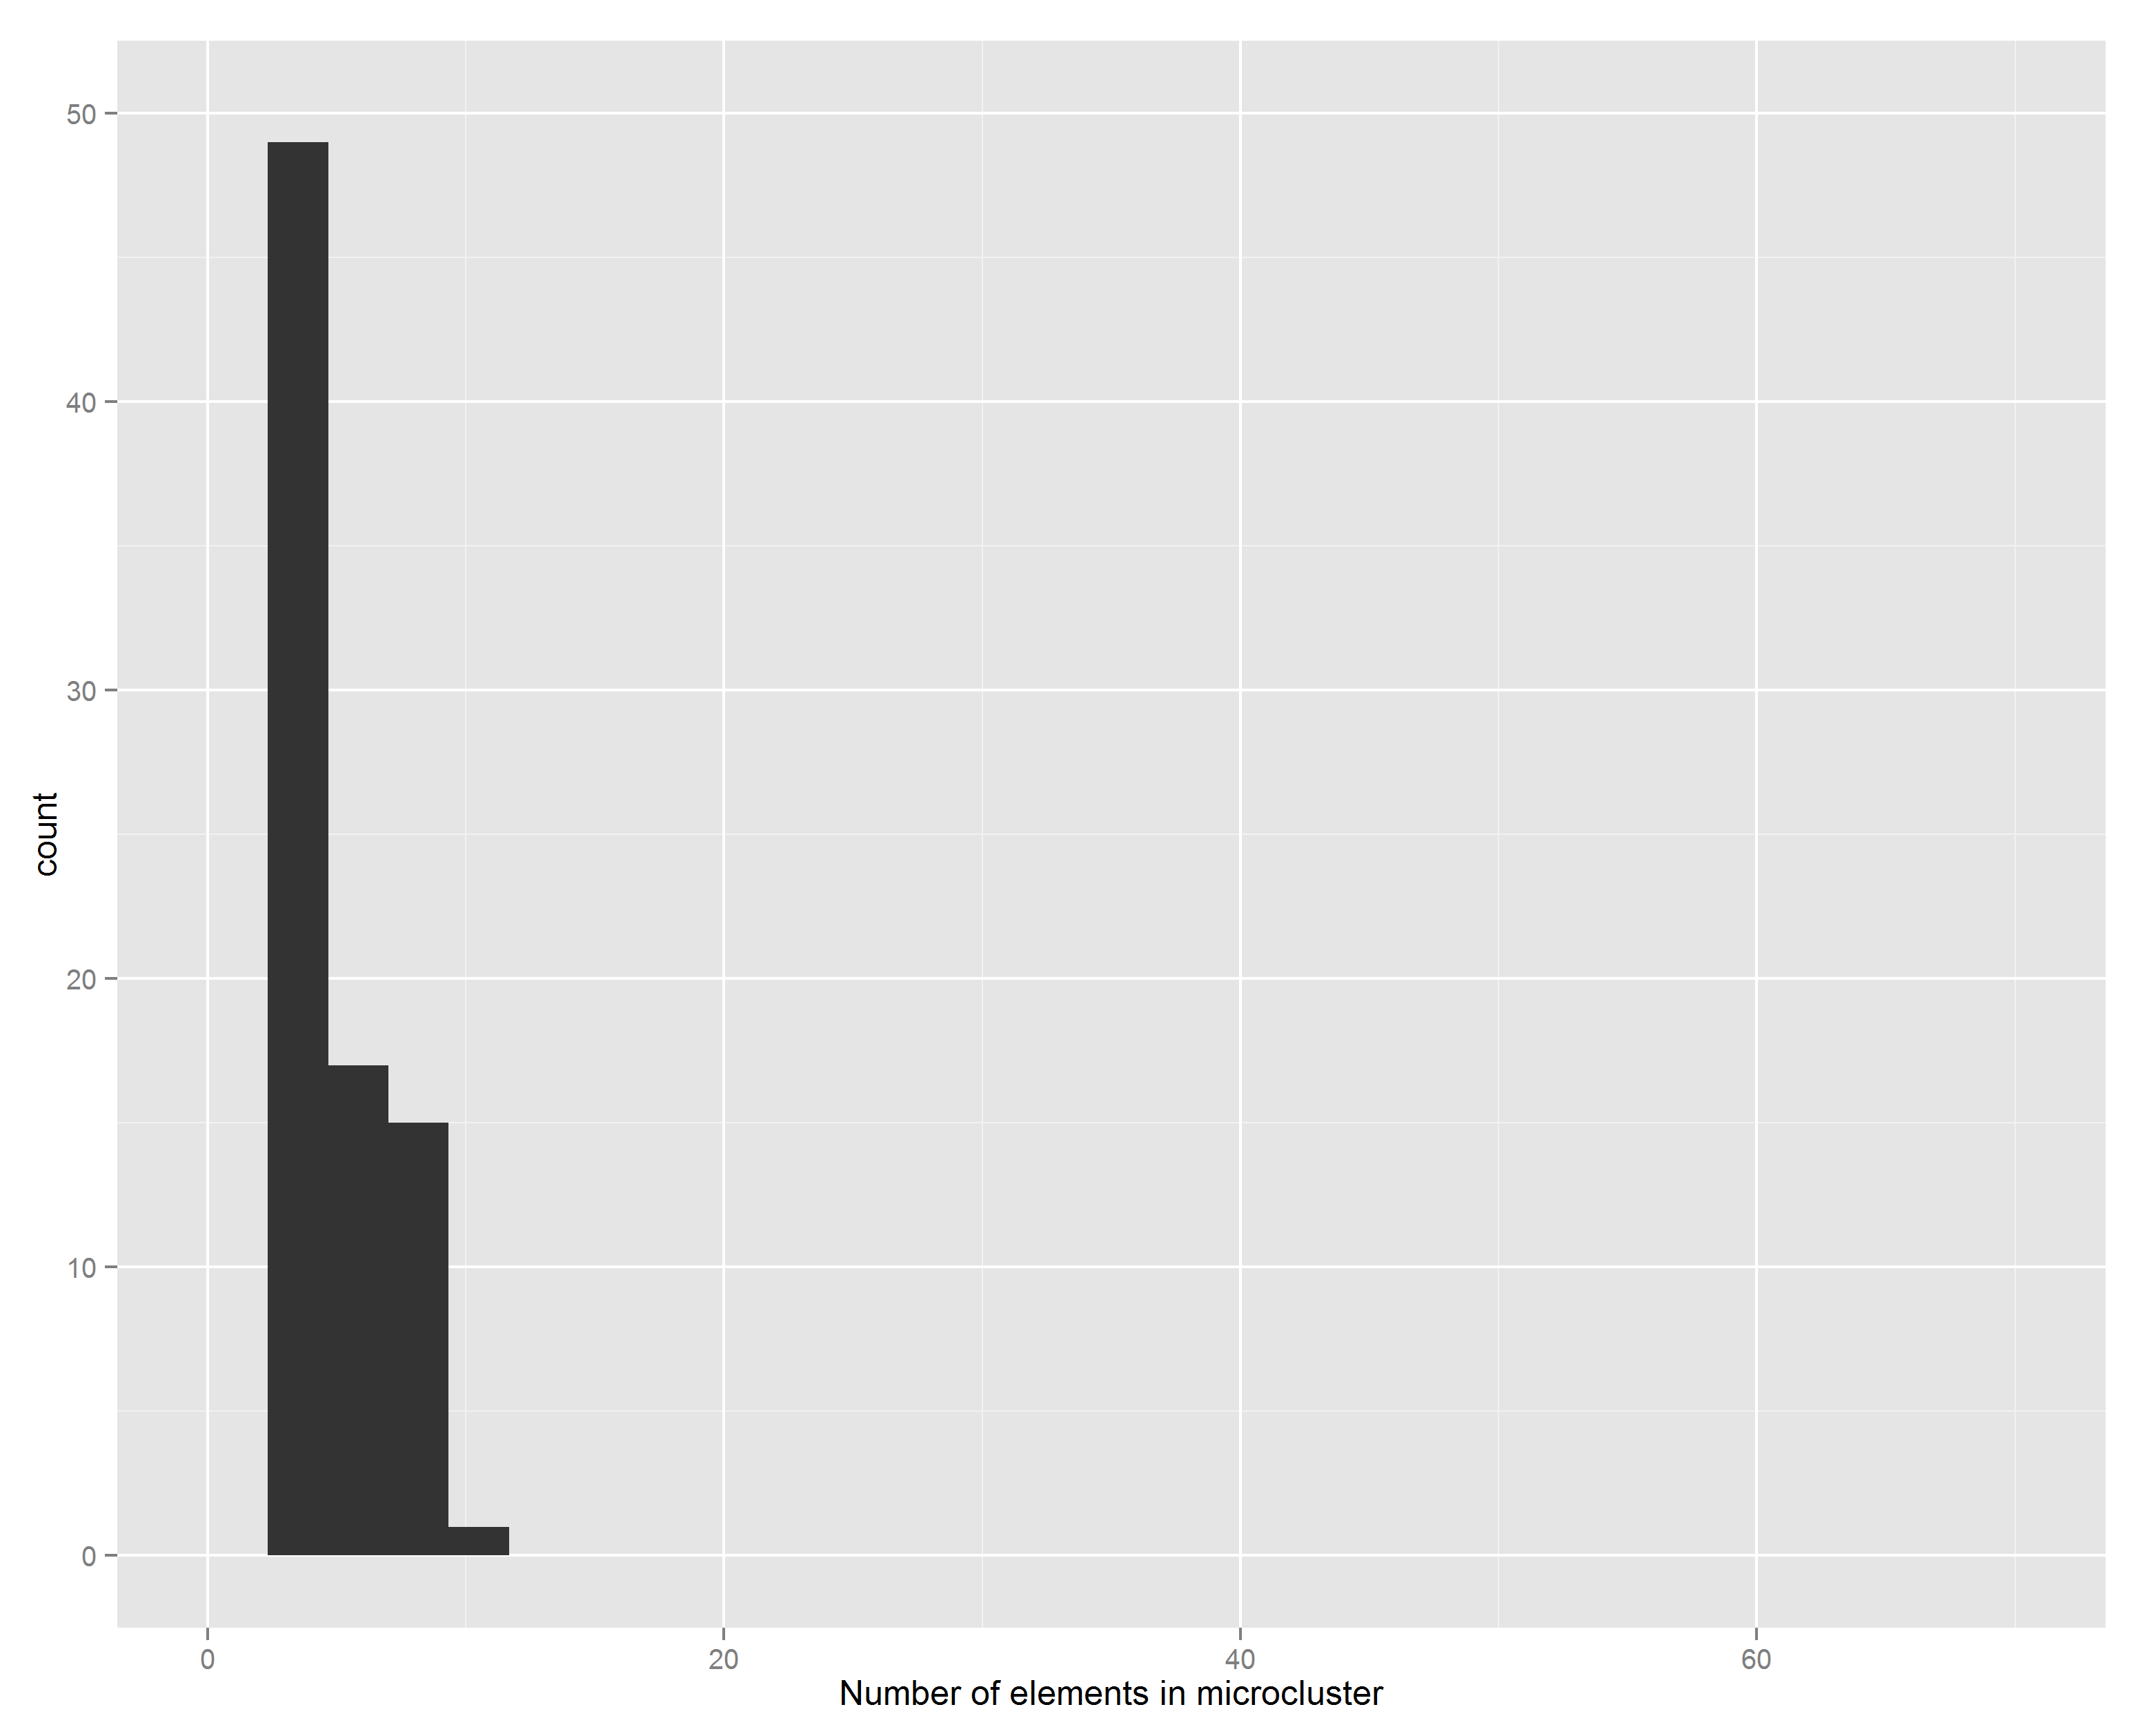
\includegraphics[width = \textwidth]{microcluster_histograms/s_set_1_hist_microclusters_time_501_fixed.png}
    \caption{Start of the stream}
  \label{fig:hist1}
  \end{subfigure}
  \begin{subfigure}{0.32\textwidth}
    \centering
    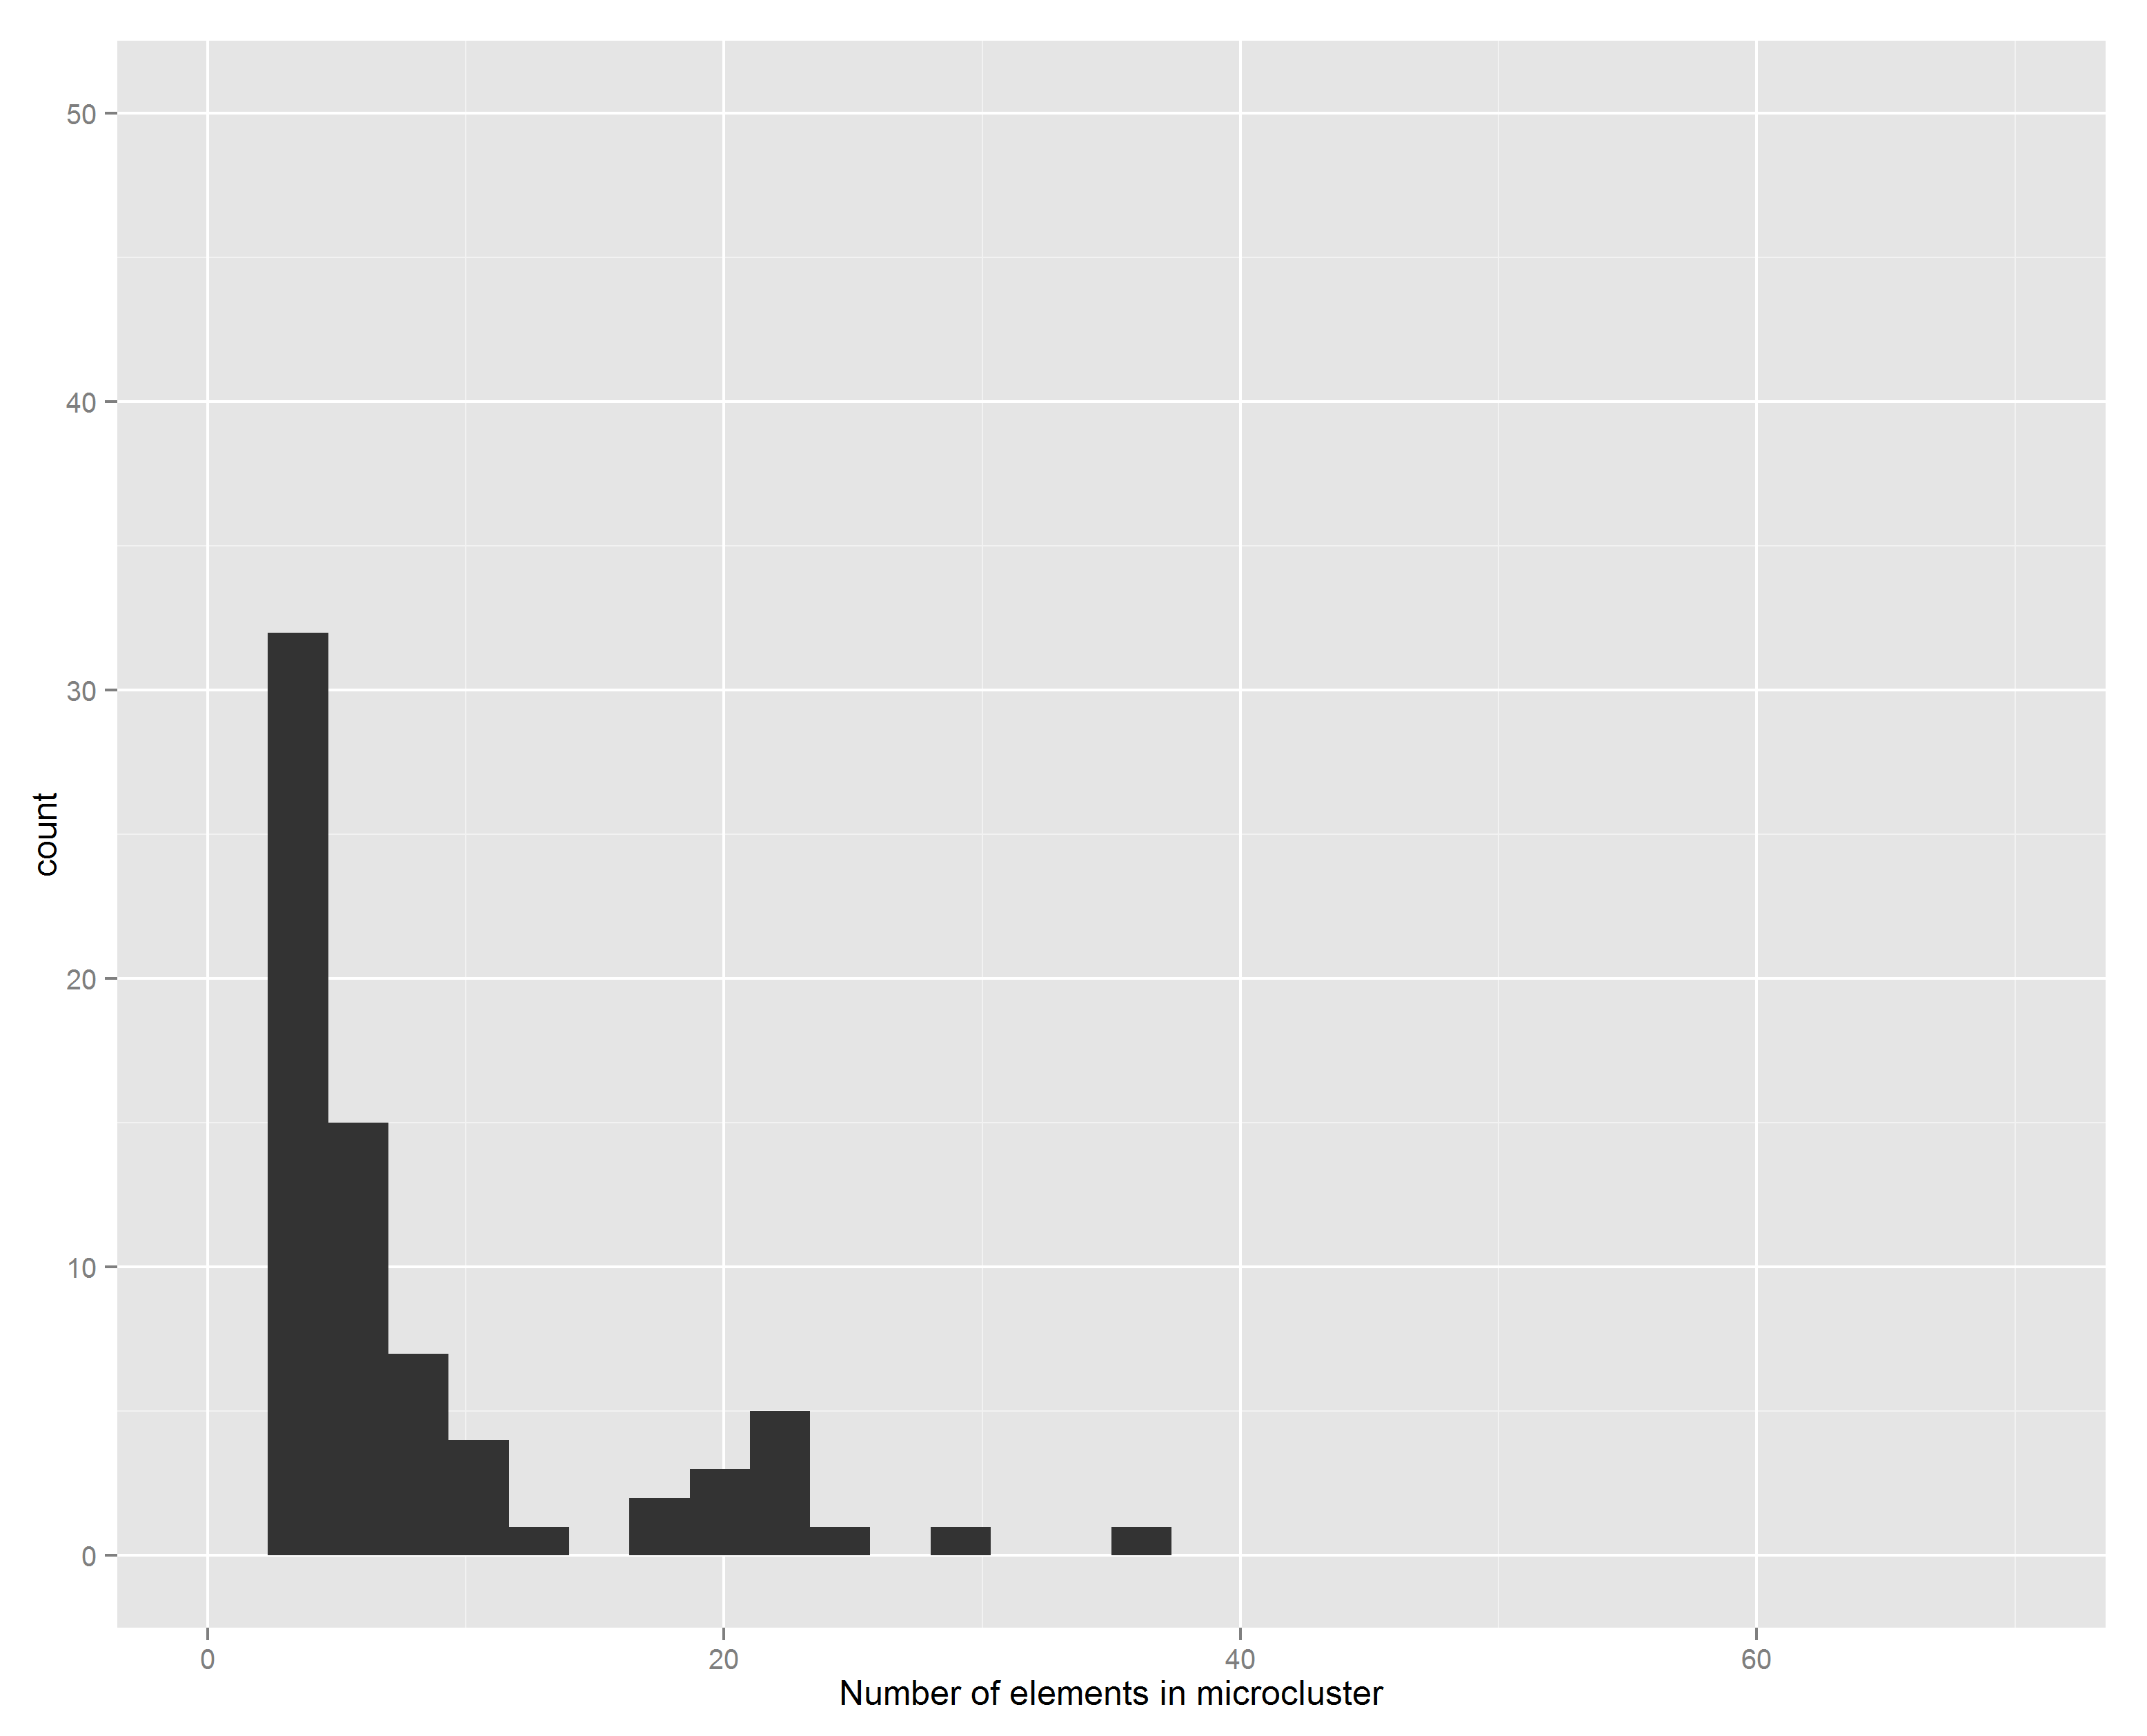
\includegraphics[width = \textwidth]{microcluster_histograms/s_set_1_hist_microclusters_time_1250_fixed.png}
  \caption{Middle of the stream}
  \label{fig:hist2}
  \end{subfigure}
\begin{subfigure}{0.32\textwidth}
    \centering
    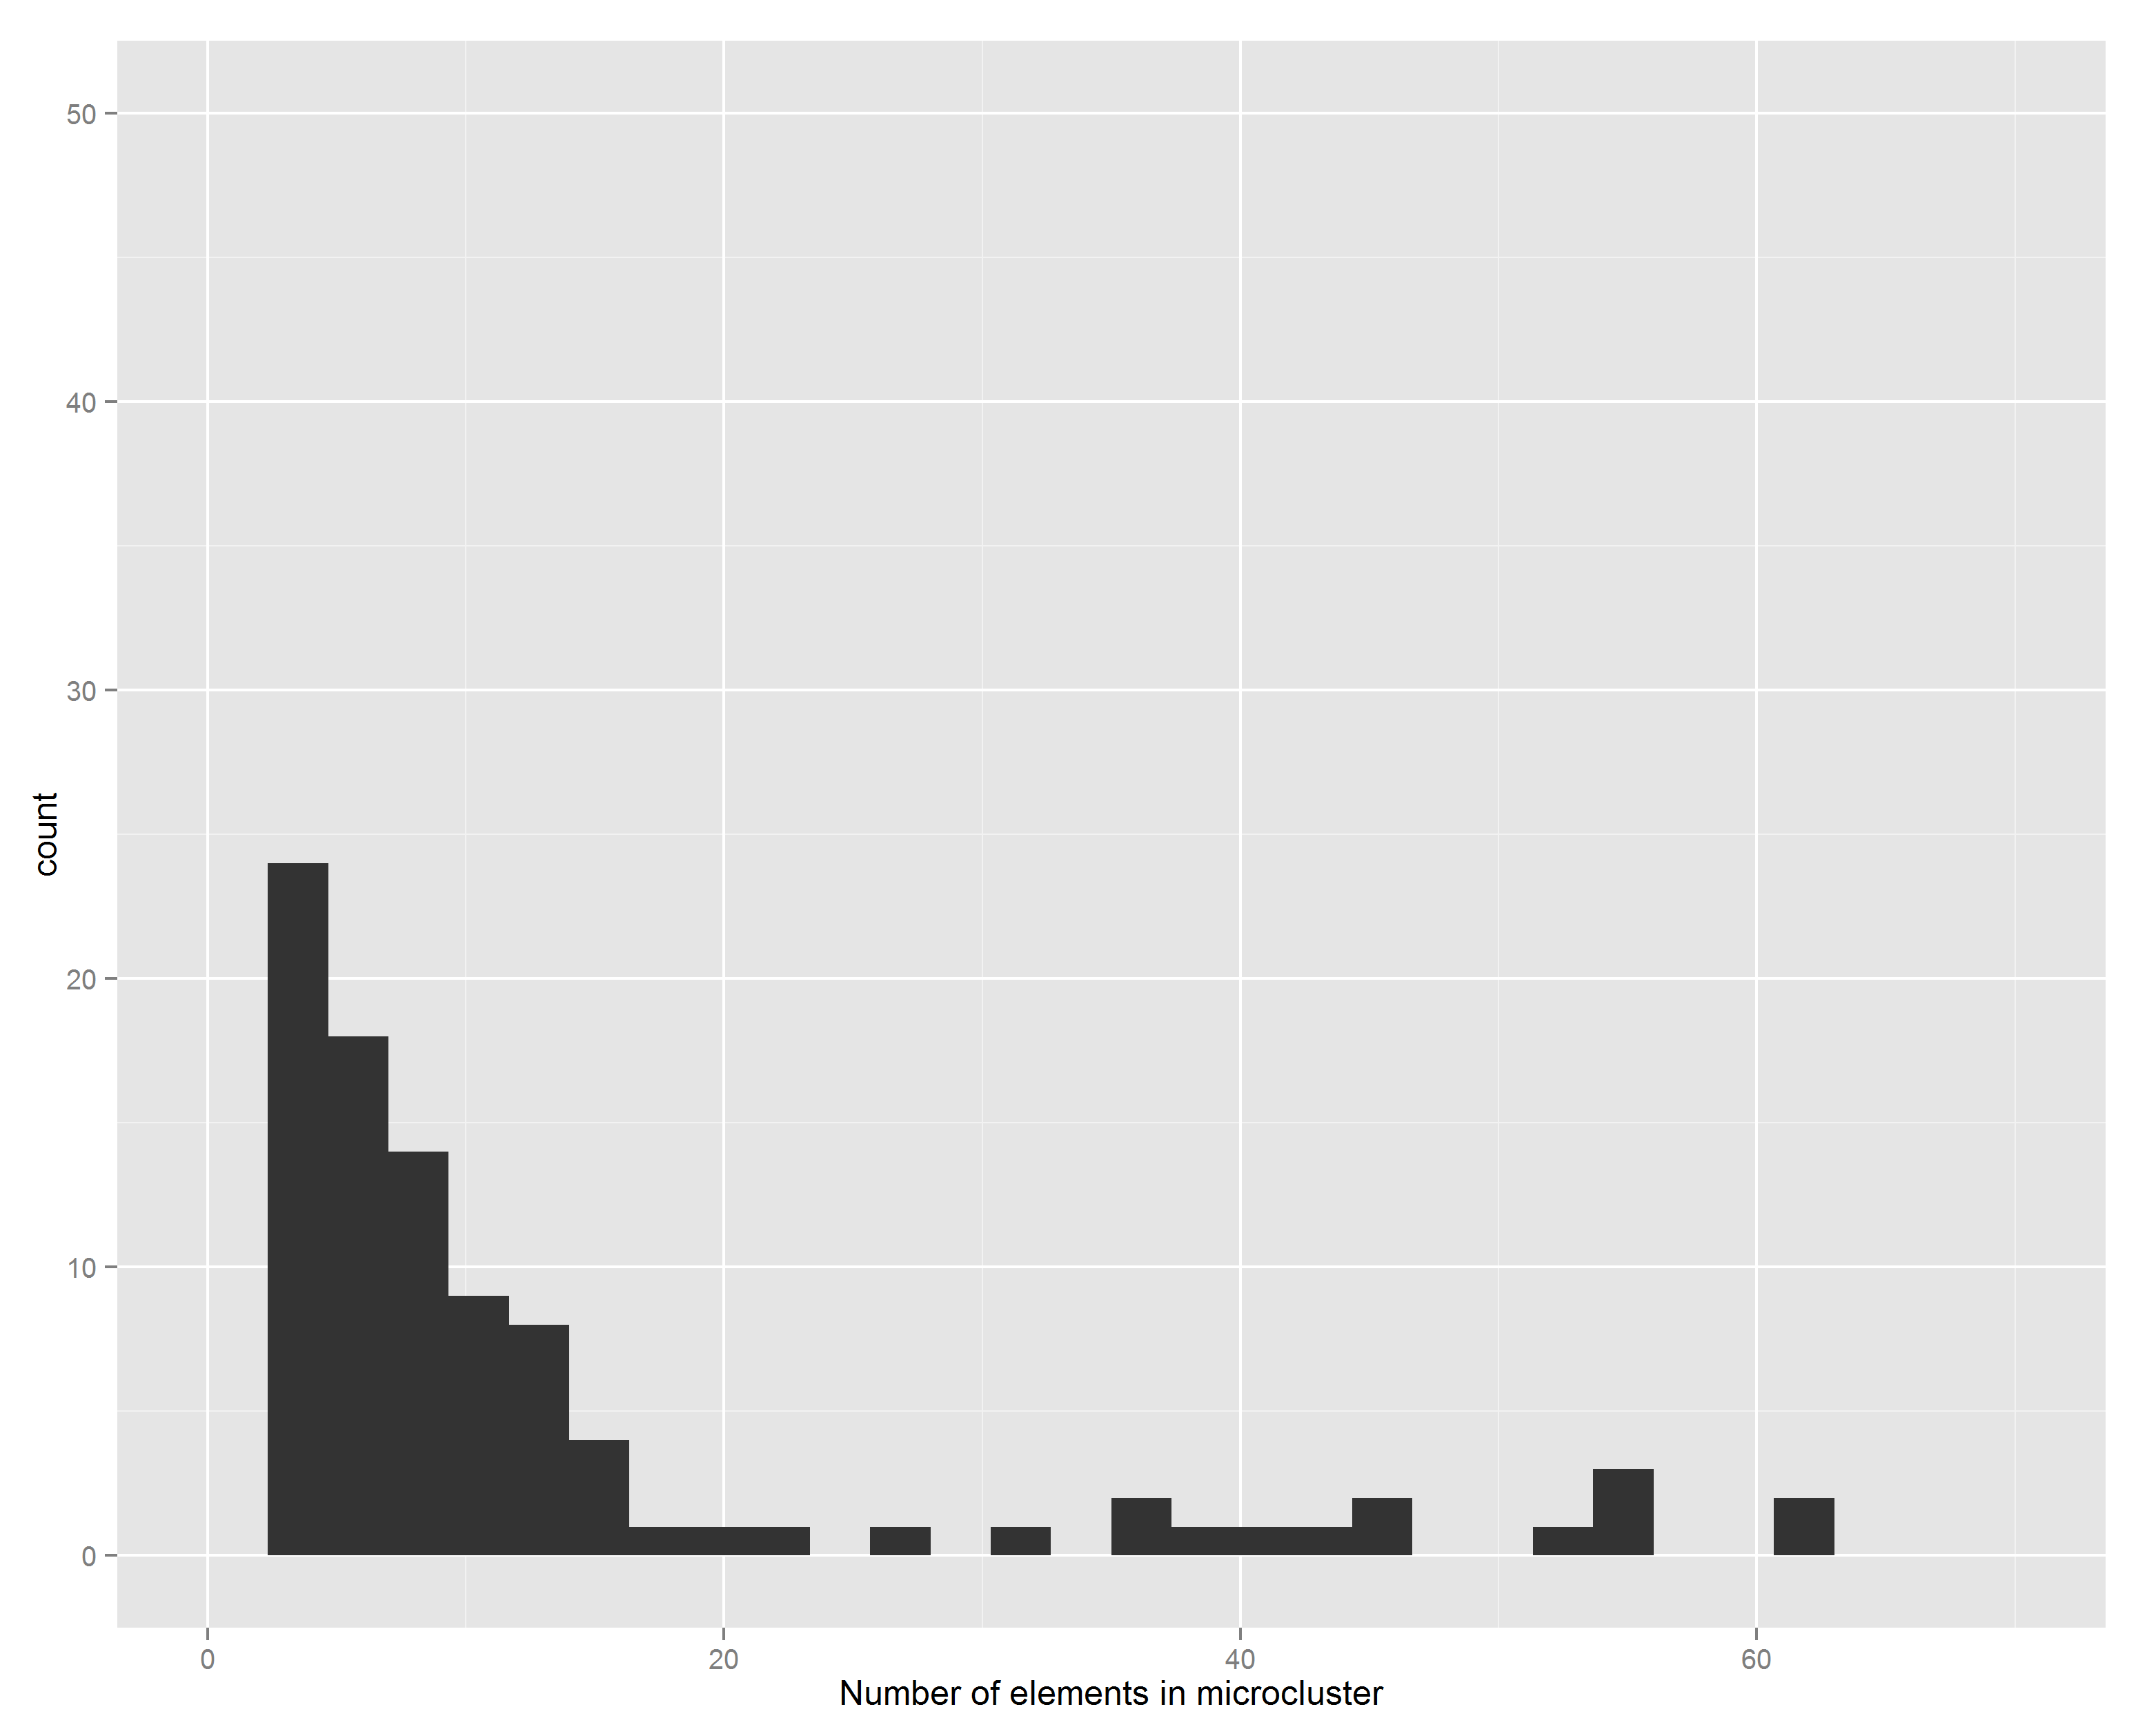
\includegraphics[width = \textwidth]{microcluster_histograms/s_set_1_hist_microclusters_time_2000_fixed.png}
  \caption{End of the stream}
  \label{fig:hist3}
  \end{subfigure}
    \caption{Histograms showing the number of points assigned to micro-clusters}
  \label{fig:microHist}
\end{figure}

Secondly, imagine the scenario pictured in Figure \ref{fig:motivate_weighting} where we have two clusters, one much more dense that then other.  In the example, many micro-clusters are used to represent the  cluster on the right, although each micro-cluster only has a few data points assigned to it. The more dense cluster in the bottom left of the plot has only 3 micro-clusters representing it, but each micro-cluster has hundred of data points assigned to it.   Weighting by the number of points assigned to a micro-cluster may help balance out this scenario for the Spectral Clustering stage. 

\begin{figure}[h]
  \centering
  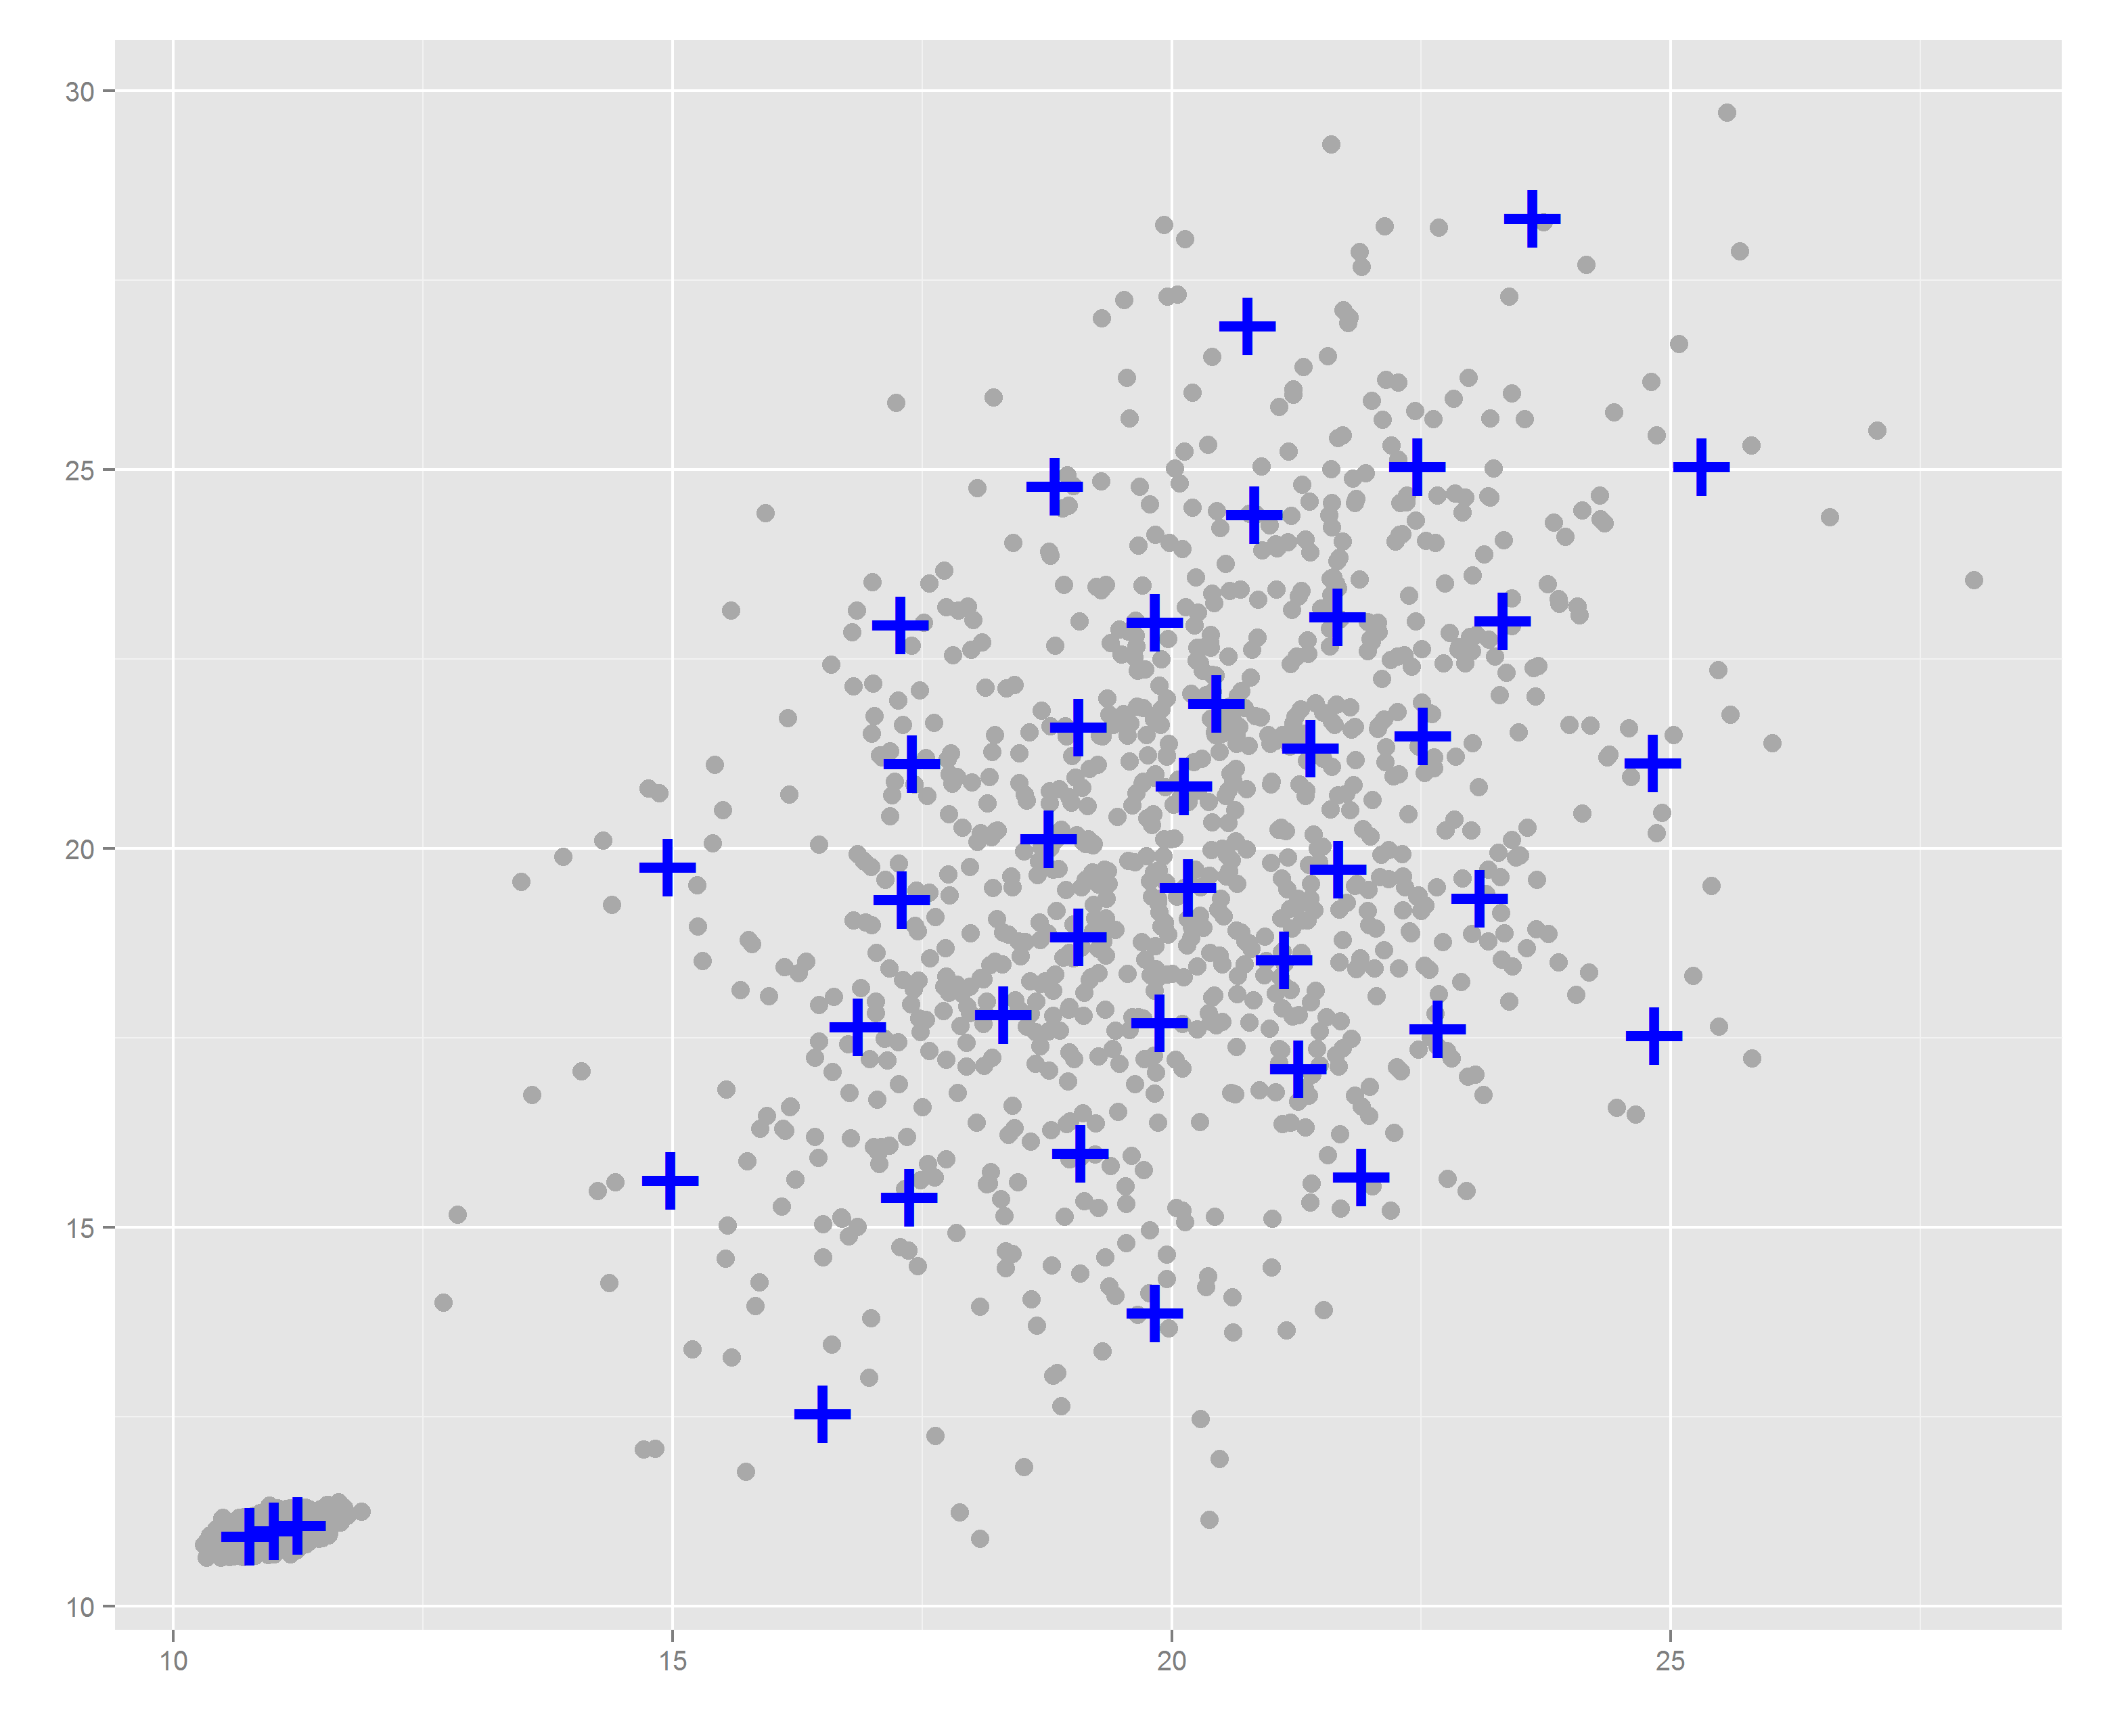
\includegraphics[width = 7cm]{motivate_weighting.png}
  \caption{Possible micro-cluster  locations in a toy example.}
\label{fig:motivate_weighting}
\end{figure}

In order to weight the the micro-clusters, we simply construct an affinity as described. 
Let $W \in \mathbb{R}^{q \times q}$ be the affinity matrix of the micro-cluster centres with $i,j$-th element equal to the similarity between micro-cluster $M_i$ and $M_j$, 

\[ W_{i,j} = \exp \left(- \frac{\| \bar{M_i} - \bar{M_j}\|^2}{2 \sigma^2} \right), \quad i, j = 1, \ldots, q. \]

Define the \textit{weighted affinity matrix} to be $\tilde{W} \in \mathbb{R}^{q \times q}$ where $ \tilde{W_{ij}} = n_in_jW_{ij}$. We can see that $\tilde{W}$ is a valid affinity matrix since it is symmetric with non-negative entries. If we wish to have $\tilde{W}_{ij} \leq 1$ then simply divide $\tilde{W}$ by $\argmax_i n_i^2$, but this makes no difference to the spectral decomposition \citep{Luxburg2008}. 

There exists a link between the spectral decomposition of  the Laplacian generated by $\tilde{W}$ and the Laplacian arising from a data set of repeated points, which we define as follows.  Let $W^* \in \mathbb{R}^{n \times n}$ be the repeated affinity matrix with the micro-cluster centres repeated based on the number of points assigned to them. Assume that the columns (and therefore rows) of $W^*$ are ordered such that the first $n_1$ are associated with the data assigned to micro-cluster 1, which has size $n_1$ and the next $n_2$ with those assigned to micro-cluster 2, and so on. Let $D, \tilde{D}, D^{*},$ be the corresponding degree matrices and $L, \tilde{L}, L^{*}$ be the corresponding normalised symmetric Laplacians.

Lets consider the Affinity and Laplacian matrices more closely for a very simple case. Assume that we have two micro-clusters, $M_1$ and $M_2$,  which have $n_1$ and $n_2$ points assigned to them respectively. Let the similarity between the two micro-cluster centres be $s$, and assume that we are using the standard Gaussian kernel to generate affinity matrices, so therefore the diagonal elements will be equal to 1. The affinity, degree and Laplacian matrices ($W$,$D$ and $L$) for the two micro-cluster centres are given in equation \eqref{eq:example_centers}.

\begin{equation}
  \label{eq:example_centers}
 W = \left(
  \begin{array}{cc}
    1 & s \\
    s & 1
  \end{array} \right), \quad
%
 D = \left(
  \begin{array}{cc}
    1+s & 0 \\
    0 & 1+s
  \end{array} \right), \quad
%
 L_{\text{symm}} = \left(
  \begin{array}{cc}
    \frac{1}{1+s} & \frac{s}{1+s} \\
    \frac{s}{1+s} & \frac{1}{1+s} 
  \end{array} \right) 
\end{equation}

In order to create a weighted version of the affinity matrix, we simply multiply through by $n_1$ and $n_2$. The weighted affinity matrix $\tilde{W}$ and related degree and Laplacians ($\tilde{D}$ and $\tilde{L}$) are given in equation \eqref{eq:example_weighted}.% We can see how this is incorporated into the Laplacian. Note that we are working with the Symmetric Normalised Laplacian. In order to weight in this manner for the unnormalised Laplacian a scaling of the diagonal matrix is would be required  \citep{Luxburg2008}.

\begin{equation}
\begin{gathered}
 \tilde{W} = \left(
  \begin{array}{cc}
    n_1^2 & sn_1n_2 \\
    sn_1n_2 & n_2^2
  \end{array} \right) , \quad 
%
 \tilde{D} = \left(
  \begin{array}{cc}
    n_1^2 + sn_1n_2 & 0 \\
    0 & n_2^2 + sn_1n_2
  \end{array} \right) \\ \\ 
 \tilde{L}_{\text{symm}} = \left(
  \begin{array}{cc}
   \frac{n_1^2}{n_1^2+sn_1n_2} & \frac{sn_1n_2}{\sqrt{(n_1^2+sn_1n_2)(n_2^2+sn_1n_2)}} \\
   \frac{sn_1n_2}{\sqrt{(n_1^2+sn_1n_2)(n_2^2+sn_1n_2)}} &  \frac{n_2^2}{n_2^2+sn_1n_2}
  \end{array} \right) \\
\end{gathered} \label{eq:example_weighted} 
\end{equation}

Finally we observe the construction of the repeated affinity matrix given in equation \eqref{eq:example_repeated}. Here the block nature in $W^*$, $D^*$ and $L^*$ is clear. The first $n_1$ rows of $W^*$ relate to the centre of micro-cluster 1, and the bottom $n_2$ rows relate to the centre of micro-cluster 2.

\begin{equation}
\begin{gathered}
  W^* = \left(
  \begin{array}{cccccc}
    1 & \hdots & 1 & s & \hdots & s \\
    \vdots & \ddots & \vdots & \vdots & \ddots & \vdots \\
    1 & \hdots & 1 & s & \hdots & s \\
   s & \hdots & s & 1 & \hdots & 1 \\
    \vdots & \ddots & \vdots & \vdots & \ddots & \vdots \\
    s & \hdots & s & 1 & \hdots & 1 
  \end{array} \right) , \quad 
%
 D^* = \left(
  \begin{array}{cccccc}
    \star & 0 & 0 & 0 & \hdots & 0 \\
    0 & \ddots & 0 & \vdots & \ddots & \vdots \\
    0 & 0 & \star & 0 & \hdots & 0 \\
   0 & \hdots & 0 & \bigtriangleup & 0 & 0 \\
    \vdots & \ddots & \vdots & 0 & \ddots & 0 \\
    0 & \hdots & 0 & 0 & 0 & \bigtriangleup 
  \end{array} \right) \\
%
 L_{\text{symm}}^* = \left(
  \begin{array}{cccccc}
    \frac{1}{\star} & \hdots & \frac{1}{\star} & \frac{s}{\sqrt{\star \bigtriangleup}} & \hdots & \frac{s}{\sqrt{\star \bigtriangleup}} \\
    \vdots & \ddots & \vdots & \vdots & \ddots & \vdots \\
    \frac{1}{\star} & \hdots & \frac{1}{\star} & \frac{s}{\sqrt{\star \bigtriangleup}} & \hdots & \frac{s}{\sqrt{\star \bigtriangleup}} \\
   \frac{s}{\sqrt{\star \bigtriangleup}} & \hdots & \frac{s}{\sqrt{\star \bigtriangleup}} & \frac{1}{\bigtriangleup}  & \hdots &  \frac{1}{\bigtriangleup} \\
    \vdots & \ddots & \vdots & \vdots & \ddots & \vdots \\
    \frac{s}{\sqrt{\star \bigtriangleup}} & \hdots & \frac{s}{\sqrt{\star \bigtriangleup}} & \frac{1}{\bigtriangleup}  & \hdots &  \frac{1}{\bigtriangleup} 
  \end{array} \right) 
\\
\text{where } \star = n_1 + n_2s \text{ and } \bigtriangleup = n_1s + n_2. 
\end{gathered} \label{eq:example_repeated}
\end{equation}

If we evaluate these expressions for a particular numerical case, we can see how the spectral decomposition of the matrices $\tilde{L}$ and $L^* $are linked.

Let $s = 0.5$, $n_1 = 3$, $n_2 = 2$. The 2nd smallest eigenvector of $L^*_{\text{symm}}$ is 

\begin{equation}
  \label{eq:e2*}
   e_2^* = \left[ 
\begin{array}{ccccc}
  -0.350& -0.350& -0.350& 0.562& 0.562  
\end{array} \right].
\end{equation}

The 2nd smallest eigenvector of $\tilde{L}_{\text{symm}}$ is 

\begin{equation}
  \label{eq:e2}
   \tilde{e}_2 = \left[ 
\begin{array}{cc}
  0.607 & -0.795 \\
\end{array} \right] .
\end{equation}

If we expand the eigenvector $\tilde{e}_2$ by expanding it's elements and block dividing by $\sqrt{n_1}$ and $\sqrt{n_2}$ respectively, we get the following, 
\begin{equation}
  \label{eq:e_repeat}
   \left[ \; \overbrace{\frac{0.607}{\sqrt{3}} \; \frac{0.607}{\sqrt{3}} \; \frac{0.607}{\sqrt{3}}}^{n_1} \; \overbrace{\frac{-0.795}{\sqrt{2}} \; \frac{-0.795}{\sqrt{2}}}^{n_2} \; \right] 
=  \left[ 
\begin{array}{ccccc}
0.350& 0.350& 0.350 & -0.562& -0.562  
\end{array} \right] .
\end{equation}

We can see that the right hand vector in equation \eqref{eq:e_repeat} is the negative of the 2nd smallest eigenvector of $L^*_{\text{symm}}$, $e_2^* $ (equation \eqref{eq:e2*}). 
In fact, we will always have that the expanded repeated eigenvector of the weighted Laplacian equal to either $e_k^*$ or $-e_k^*$ for all $k$.

\RD{Nicos - Please can you help me explain the following proof better? } 
Generally, the spectral decomposition of $L^*$ and $\tilde{L}$ are linked in this way, and therefore the partition generated by performing Spectral Clustering on the weighted micro-cluster centers will be the same as the partition generated by performing Spectral Clustering on a set of repeated micro-cluster centers. We do not show a full proof for this here but sketch out the proof showing that the second smallest eigenvectors are linked in this way. 

 Let $\tilde{u}$ be the second smallest eigenvector of $\tilde{L}$.  Define $u^* =  \left( \overbrace{\frac{\tilde{u}_1}{\sqrt{n_1}}, \; \frac{\tilde{u}_1}{\sqrt{n_1}}, \; \frac{\tilde{u}_1}{\sqrt{n_1}}}^{n_1}, \; \hdots, \overbrace{\frac{\tilde{u}_k}{\sqrt{n_k}}, \; \frac{\tilde{u}_k}{\sqrt{n_k}}}^{n_k} \right)$.  We wish to show that $u^*$ is the second smallest eigenvector of $L^*$.  First we will show that $u^*$ satisfies the following criteria, 
%We can see that $\|u^*\|^2 = \sum_{i = 1}^{n}(u_i^*)^2 = \sum_{i=1}^{k}n_i \cdot \frac{\tilde{u}_i^2}{n_i} = \sum_{i = 1}^{k} \tilde{u}^2_i = 1$. 

\begin{itemize}
\setlength\itemsep{0.5em}
\item[(i)] $ \|u^*\| = 1 $
\item[(ii)] $u^* \perp D^{* 1/2} \mathds{1}$
\item[(iii)] $u^{*\top} L^* u^* = \tilde{u}^{\top} \tilde{L} \tilde{u}$
\end{itemize}

%Part (i) checks that $u^*$ has size 1 which is required for eigenvectors. Part (ii) checks that $u$ is orthogonal to the smallest eigenvector. Part (iii) shows that. 
Part(i)\\
\begin{align*}
 \|u^*\|^2 &= \sum_{i=1}^{n}u^{* 2}_i \\
&= \sum_{i = 1}^{k}n_i \frac{\tilde{u}_i^2}{n_i} \\
&= \sum_{i=1}^{k}\tilde{u}_i^2 = 1 
\end{align*}
since $\tilde{u}$ is an eigenvector. Therefore $\|u^*\| = 1$. 
 

Part (ii) \\
\begin{align*}
 \sum_{i=1}^nu^*_i D_{ii}^{* 1/2} &= \sum_{i=1}^k n_i \frac{\tilde{u}_i}{\sqrt{n_i}} \frac{\tilde{D}^{1/2}_{ii}}{\sqrt{n_i}} \\
&= \sum_{i=1}^k \tilde{u}_i \tilde{D}^{1/2}_{ii} = 0
\end{align*}
since $\tilde{u} \perp \tilde{D}^{1/2} \mathds{1}$, therefore $u^* \perp D^{* 1/2} \mathds{1}.$ 

Part (iii) \\
First we state the general property given in \cite{Luxburg2008} for the normalised Laplacian. For every $f \in  \mathbb{R}^n$ we have
\begin{equation}
  \label{eq:luxburg_vectors}
  f^{\prime} L_{\text{symm}}f = \frac{1}{2} \sum_{i,j=1}^n w_{ij} \left( \frac{f_i}{\sqrt{d_i}} - \frac{f_j}{\sqrt{d_j}}  \right)^2.
\end{equation}

Using this property, 
\begin{align*}
  \tilde{u}^{\top} \tilde{L} \tilde{u} &= \frac{1}{2} \sum_{i = 1}^k \sum_{j = 1}^k \left( \frac{\tilde{u}_i}{\sqrt{\tilde{D}_{ii \phantom{j}}}} - \frac{\tilde{u}_j}{\sqrt{\tilde{D}_{jj}}}  \right)^2 \tilde{W}_{ij} \\
 &= \frac{1}{2} \sum_{i = 1}^k \sum_{j = 1}^k \left( \frac{\tilde{u}_i / \sqrt{n_i}}{\sqrt{D_{ii}}} - \frac{\tilde{u}_j / \sqrt{n_j}}{\sqrt{D_{jj}}} \right)^2 n_i n_j  W_{ij}
  %&= \frac{1}{2} \sum_{i = 1}^k \sum_{j = 1}^k \left( \frac{\tilde{u}_i}{\sqrt{\sum_{l=1}^kn_ln_iA^{\prime}_{ij}}} - \frac{\tilde{u}_j}{\sqrt{\sum_{l=1}^kn_ln_jA^{\prime}_{ij}}} \right)^2 \tilde{A}^{\prime}_{ij}
\end{align*}
which we can see is equal to $ u^{* \top}L^*u^*$ by observing that $W^*$ has repeated elements from $W$.

Now that all of the above criteria have been satisfied, we know that $u^*$ is an eigenvector of $L^*$ and is orthogonal to the smallest eigenvector. Assume there exists some $v^*$ such that $v^* \perp D^{* 1/2}\mathds{1}$ with $\|v^*\|=1$ and $v^{* \top}L^*v^* < u^{* \top}L^*u^*$. Then $\exists \; \tilde{v}$ with $\tilde{v}^{\top} \perp \tilde{D}^{1/2}\mathds{1}$ and $\tilde{v}^T \tilde{L} \tilde{v} < \tilde{u}^{\top} \tilde{L} \tilde{u}$. This contradicts the fact that $\tilde{u}$ is the second smallest eigenvector of $\tilde{L}$. Therefore $u^*$ is the second smallest eigenvector of $L^*$ \qed 
%Now we check that there does not exist some other $v^*$ which is also a eigenvector of $L^*$ which is linked to a smaller eigenvalue of $L^*$ than $u^*$. 

\section{Experimentation}
\label{sec:clustream_exp}

In this section, we investigate the performance of both Unweighted and Weighted Spectral Clustream and a simple windowed approach to Spectral Clustering. We intended to compare against some of the Incremental Spectral Clustering methods discussed in Section \ref{sec:incremental} however due to the computational costs of the methods this was not possible. First the algorithms and methodology are introduced and the performance metrics defined. Then the algorithms are compared on simulated data, two image based data sets and an evolving data set. 

\subsubsection{The Algorithms}

Spectral Clustream is given in Algorithm \ref{alg:onlineSpec}. As described in Section \ref{sec:microSpec}, there are two  ways that we can incorporate the micro-cluster centres into the macro-clustering; not weighting, or weighting. Unweighted clustream takes the micro-cluster centres as direct input into the Spectral Clustering algorithm. Weighted clustream weights the micro-cluster centres by the number of data points assigned to that micro-cluster. In both Spectral Clustream algorithms we use $q = 150$ micro-clusters to summarise the data stream.

Windowed Spectral Clustering is a simple algorithm which retains a window of only the  $w$  most recently observed data points. When a new data point is observed, the oldest data point in the window is discarded to make room for the new data point. Only the data points in the current window are available for input into a standard Spectral Clustering algorithm. We use a fixed window size of $150$ data points for the duration of the stream.

\subsection{Methodology}
\label{sec:methodology}
A data stream $S = \{ \boldsymbol{x_i} \}_{i \in \mathbb{N}}$ is observed sequentially, with one data point $\boldsymbol{x_t}$ observed at each time point.  The order in which the data stream is observed is randomised to generate 10 different runs.  Results are averaged out over these runs. 

Each run consists of four stages; initialisation, updating,  generating cluster labels and evaluation. Spectral Clustream is initialised by applying k-means with 150 clusters to the first 500 data points and applying equations \eqref{eq:microcluster_def}. When a new data point  $\boldsymbol{x_t}$ is observed the streaming algorithms are updated. In Spectral Clustream this is achieved by applying Algorithm \ref{alg:clustream}. Windowed Spectral Clustering shifts the window along by one, discarding the oldest data point $\boldsymbol{x_{(t-150)}}$ and including $\boldsymbol{x_t}$. Every ten times steps we generate cluster labels for the data stream by applying Spectral Clustering on the \textit{representative points} of the data stream. In Spectral Clustream the representative points are the micro-clusters (weight adjusted or not). In Windowed Spectral Clustering the representative points are the $w$ data points currently in the window. We then evaluate the Spectral Clustering performance on a \textit{test set} defined  to be the next 200 data points in the data stream ($\boldsymbol{x_{t+1}}$ , \ldots  $\boldsymbol{x_{t+200}}$). The test data points are first assigned to their nearest representative point using the Euclidean distance metric and then take on the cluster label of that representative point. Performance is measured in terms of purity and V-measure of the test data using the known true clusters. Purity and V-measure are defined in Section \ref{sec:performance}.

The parameter settings throughout are as follows. In Spectral Clustream algorithms we set $\delta = 0.1, m = 1$ and $ \tau = 2$. For the first three experiments we use $q = 150$ microclusters. In Section \ref{sec:non_stationary} we compare results for a number of different values of $q$. Similarly, in the first three experiments we use a window size of $w = 150$ for Windowed Spectral clustering, but investigate varying $w$ in the final experiment. In all experiments, we set the number of clusters $k$ to be equal to the known true number of classes for the data set. 

\subsection{Performance Measures}
\label{sec:performance}
The two measures that are used to quantify cluster performance are purity and V-measure, both of which are well used in the clustering literature. Both measures require knowledge of the ``true class'' of the data points, which may not always be available for real data sets.  

Let $n$ be the number of data points, $U = \left\{ u_i | 1, \ldots, k  \right\} $ be the set of true classes and $V = \left\{ v_j | 1, \ldots, k \right\}$ be the set of clusters assigned by the clustering algorithm.  Define $A$  to be  the contingency table produced by the clustering algorithm representing the clustering solution such that $a_{ij}$ is the number of points that are members of class $u_i$ and assigned to cluster $v_j$.

%Purity is the more intuitive of the two measures to understand as it quantifies how pure clusters are.
 A cluster which only contains data points associated with one true class will be given a high purity value. A cluster which consists of data points from many different true classes will receive a low purity value.  Purity is calculated as follows. For each cluster find the true class which is most prevalent in that cluster and count how many data points of that class there are in that cluster. Repeat this for all clusters, sum these counts and divide by the total number of data points. This is shown mathematically in equation \eqref{eq:purity}.

\begin{equation}
  \label{eq:purity}
  %\text{Purity} = \frac{1}{N} \sum_{k}\max_j | \omega_k \cap c_j |,
  %\text{Purity} = \frac{1}{N} \sum_{j}\max_i | k_j \cap c_i |.
  \text{Purity} = \frac{1}{n} \sum_{j = 1}^{k} \argmax_{i} (a_{ij}).
\end{equation}
Generally this is a useful measure, however if we had a data set where each data point was assigned to a different cluster then the purity would be perfect even though this isn't a particularly good clustering of the data. Purity can be unreliable if the number of clusters is much larger than the number of true classes. 

To account for this we also use the V-measure \citep{Rosenberg2007} which  takes the harmonic mean of two other performance measures, homogeneity and completeness. Homogeneity assesses if each cluster contains members of only a single class (in a similar way to purity), whilst completeness checks that all members of the same class are assigned to the same cluster. This is shown in equation \eqref{eq:vmeasure}:

\begin{equation}
  \label{eq:vmeasure}
  \text{V-measure} = 2 \frac{h \times c}{h + c} \;,
\end{equation}

where $h$ and $c$ are homogeneity and completeness measures as defined below in equation  \eqref{eq:homogeneity} and equation \eqref{eq:completeness} respectively. 

For homogeneity to be perfect, the clustering algorithm must assign only those data points that are members of a single class to a single cluster.
\begin{equation}
\label{eq:homogeneity}
  h=\left\{
  \begin{array}{@{}ll@{}}
    1  & \text{if} \;  H(U|V) = 0 \\
    1 - \frac{H(U|V)}{H(U)}, & \text{else}
  \end{array}\right.
\end{equation} 

\begin{align}
  \label{eq:H(U|V)}
H(U|V) &=  - \sum_{j=1}^{k} \sum_{i=1}^{k}\frac{a_{ij}}{N} \log \frac{a_{ij}}{\sum_{i=1}^{k}a_{ij}}\\
H(U) &=  - \sum_{i=1}^{k} \frac{\sum_{j=1}^{k}a_{ij}}{N} \log \frac{\sum_{j=1}^{k}a_{ij}}{N}
\end{align}

For perfect completeness the clustering must assign all data points which are members of a single class to a single cluster.

\begin{equation}
\label{eq:completeness}
 c=\left\{
  \begin{array}{@{}ll@{}}
    1  & \text{if} \;  H(V|U) = 0 \\
    1 - \frac{H(V|U)}{H(V)}, & \text{else}
  \end{array}\right.
\end{equation} 

\begin{align}
  \label{eq:H(V|U)}
H(V|U) &=  - \sum_{i=1}^{k} \sum_{j=1}^{k}\frac{a_{ij}}{N} \log \frac{a_{ij}}{\sum_{j=1}^{k}a_{ij}}\\
H(V) &=  - \sum_{j=1}^{k} \frac{\sum_{i=1}^{k}a_{ij}}{N} \log \frac{\sum_{i=1}^{k}a_{ij}}{N}
\end{align}

Both purity and V-measure are bound between 0 and 1, where 1 indicates perfect performance. 


\subsection{Simulated Results}

The first data sets tested are the popular S-sets, first introduced in \cite{Franti2006}. Each set consists of synthetic two-dimensional data with $n$=5000 data points and $k$=15 Gaussian clusters with different degrees of cluster overlapping.  The four data sets are shown in Figure \ref{fig:s_set_truth}. 

\begin{figure}[H]
\centering
\begin{subfigure}{.4\textwidth}
  \centering
  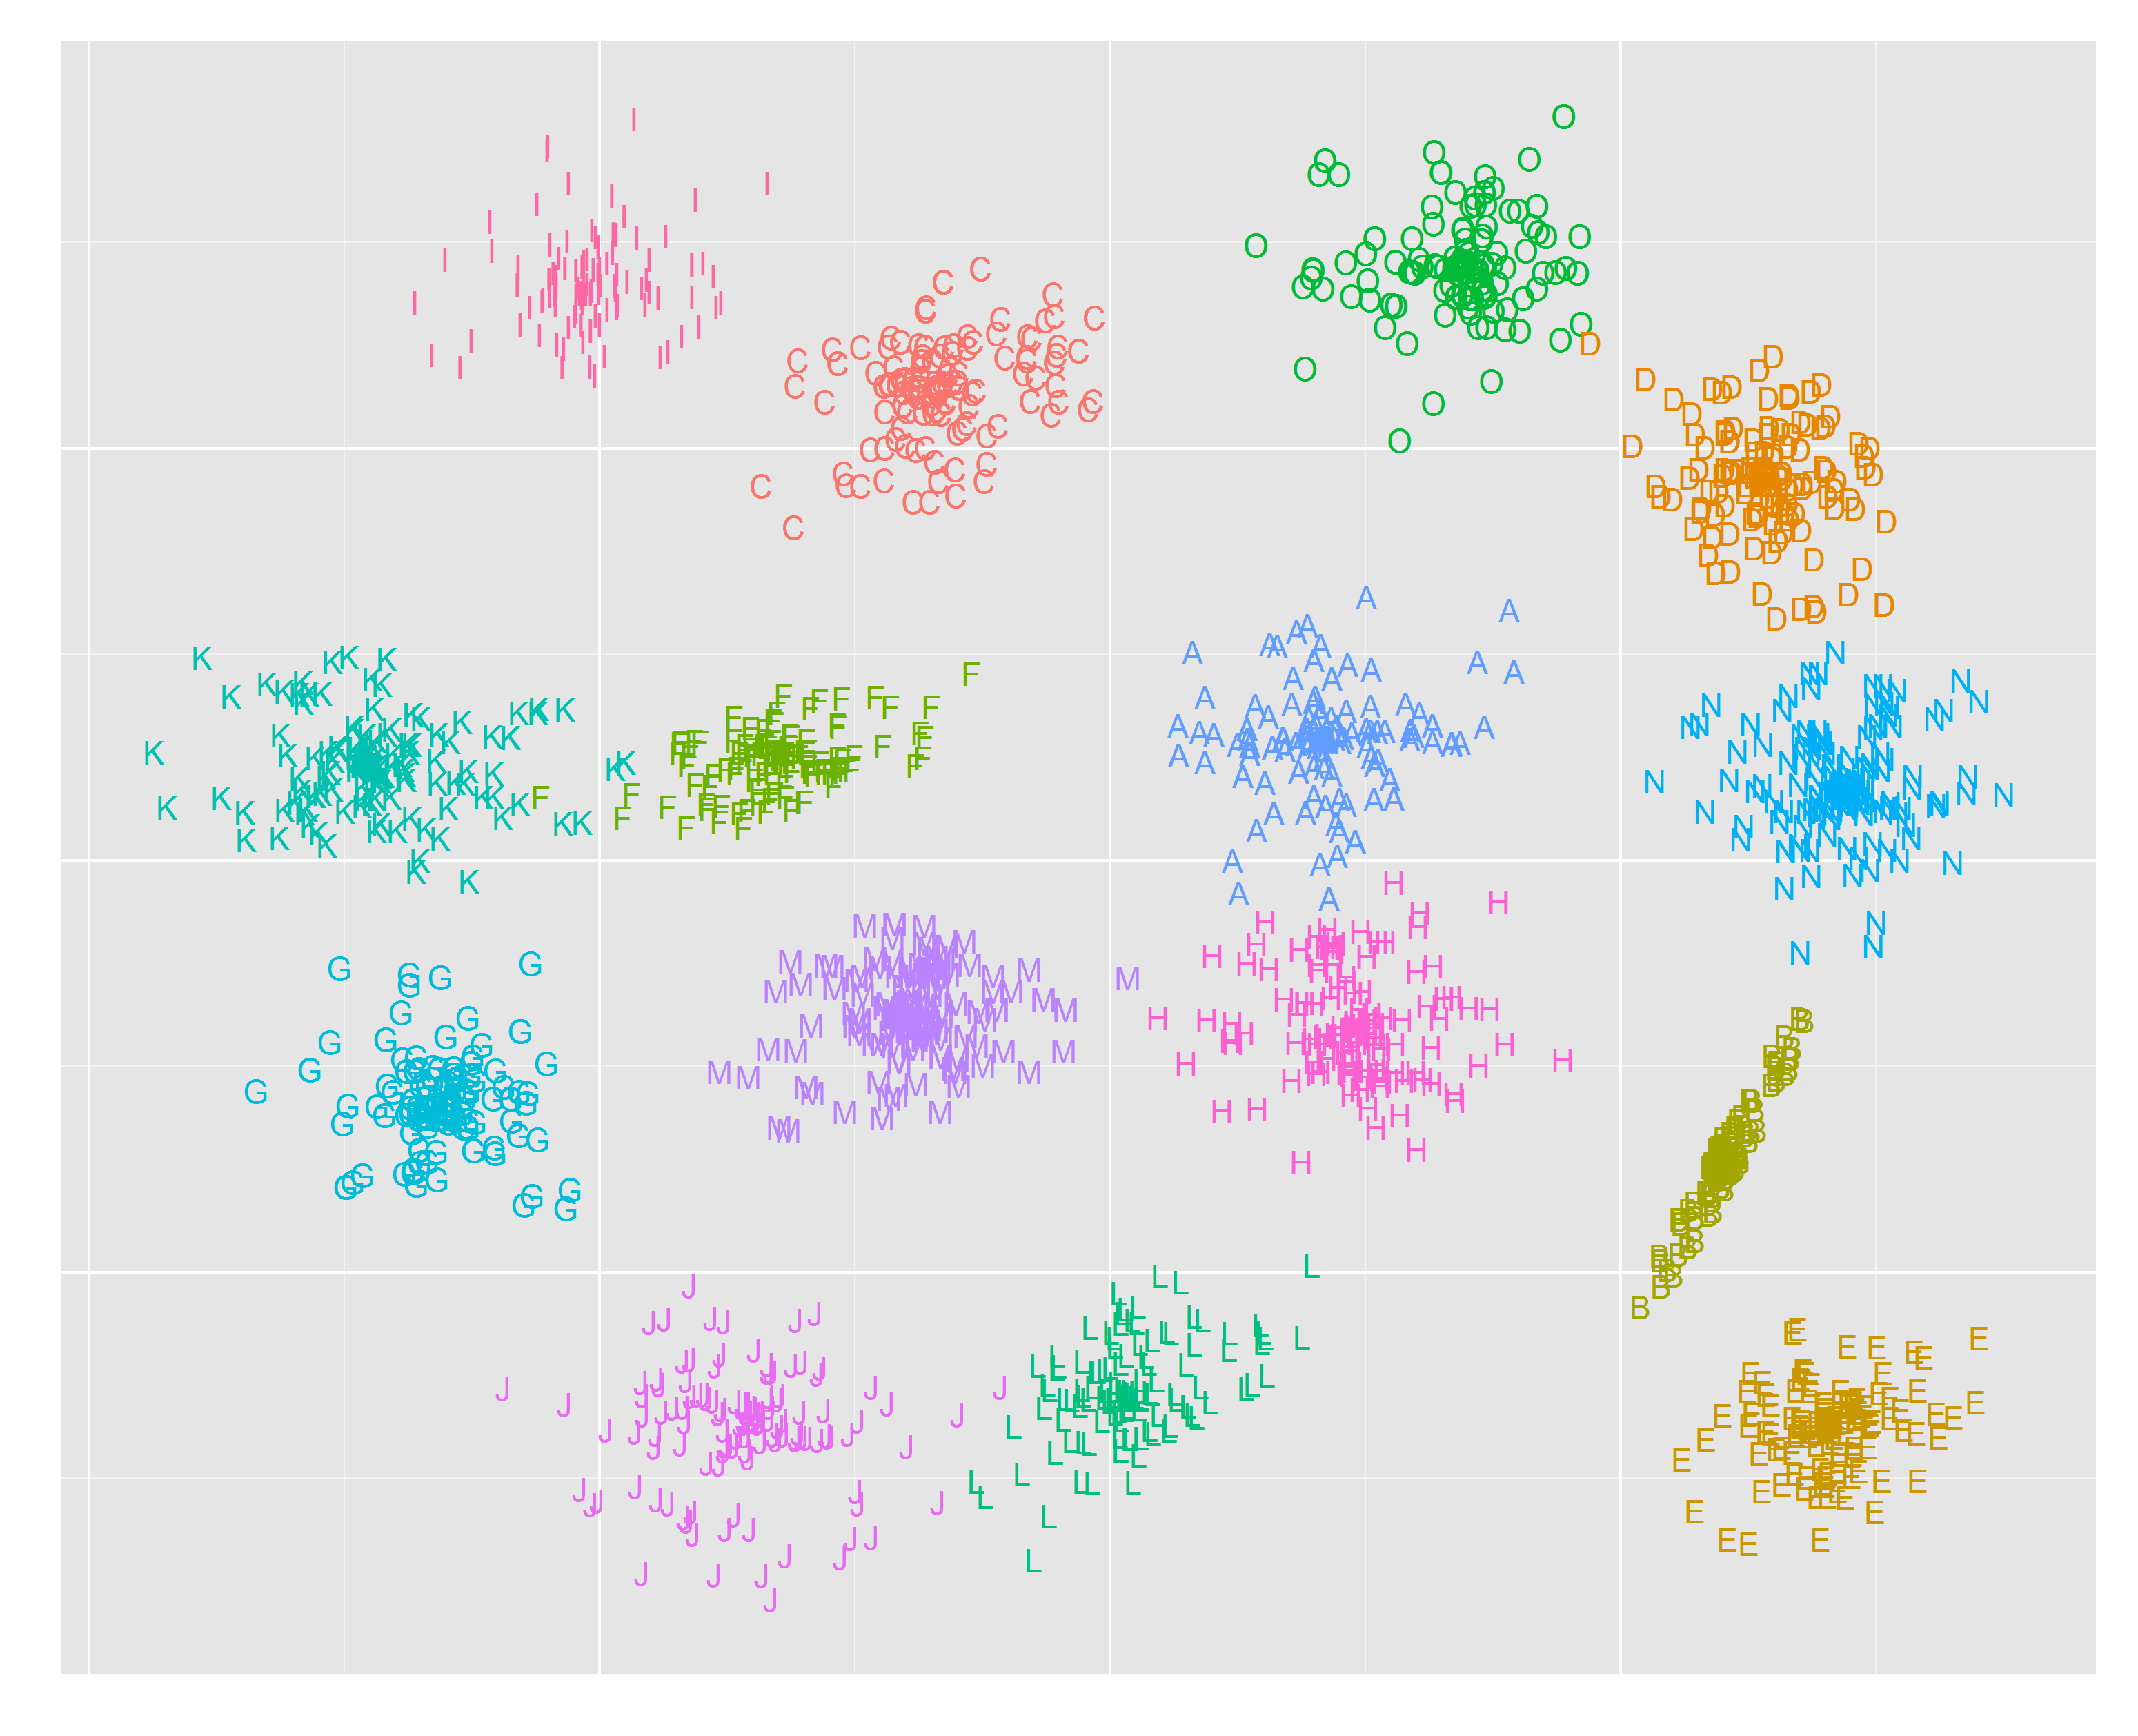
\includegraphics[width=.9\linewidth]{s_set/s_set_1_truth.png}
  \caption{S1}
 % \label{fig:sfig1}
\end{subfigure}%
\begin{subfigure}{.4\textwidth}
  \centering
  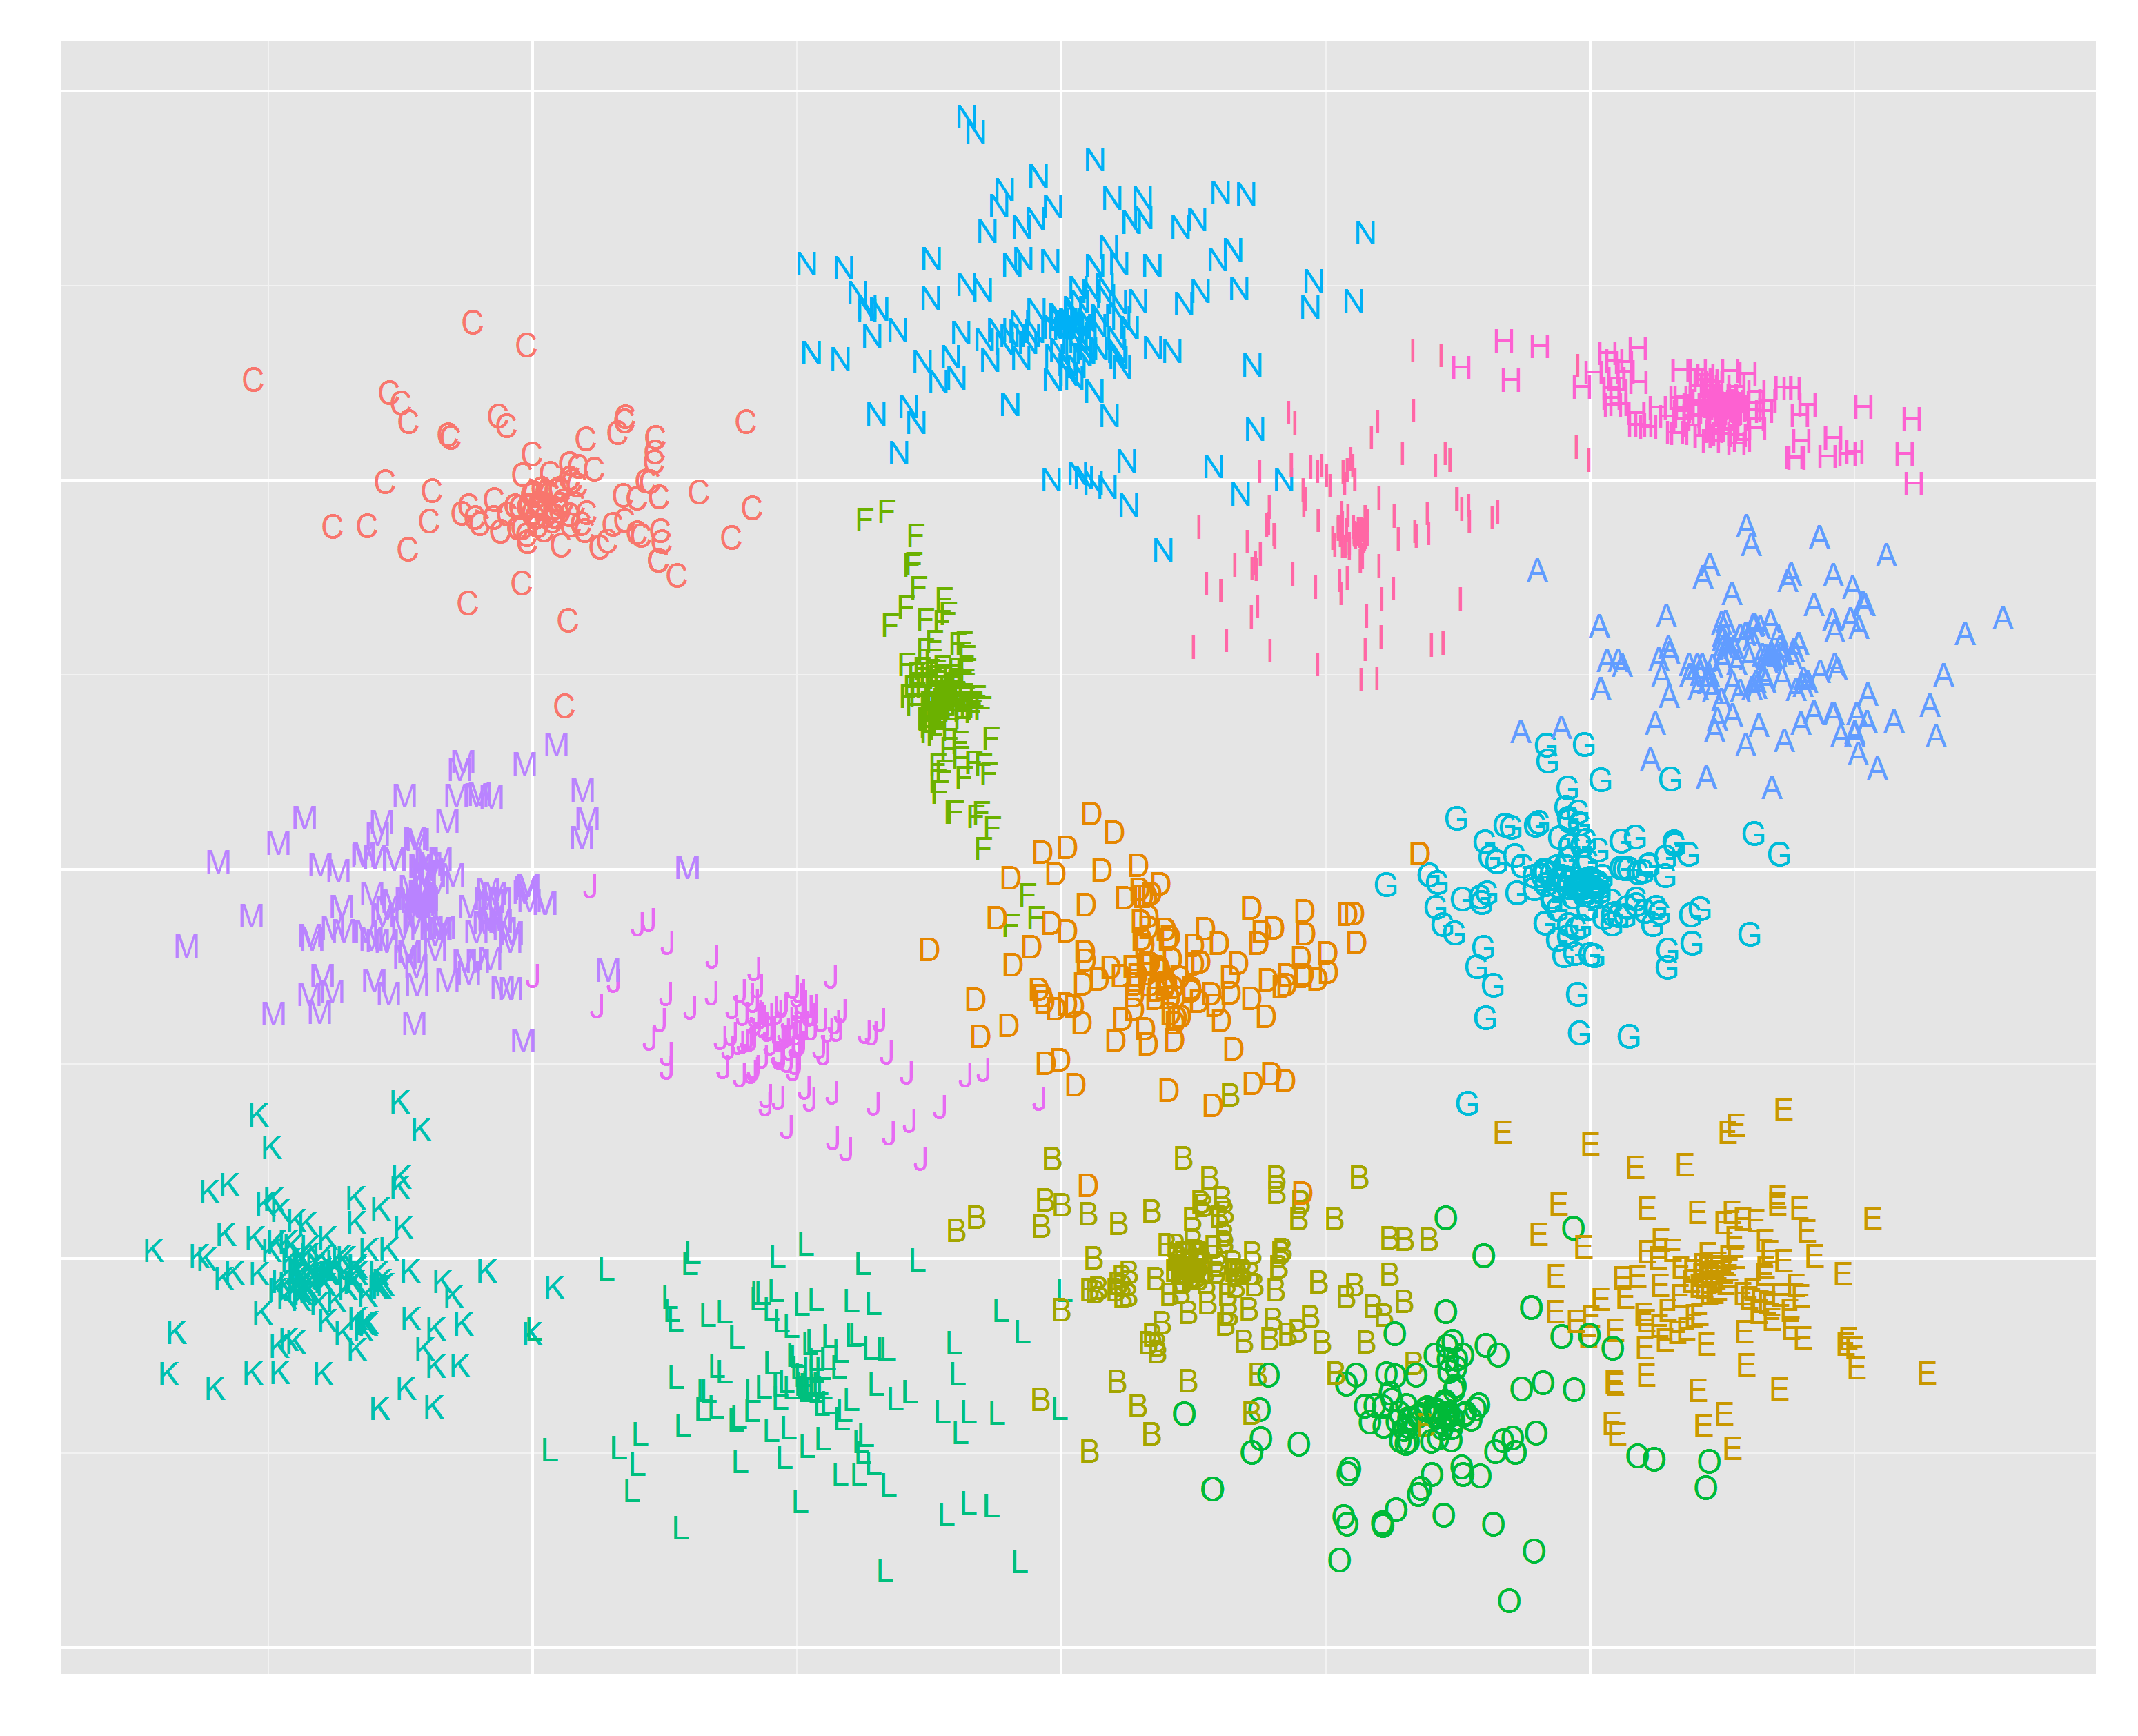
\includegraphics[width=.9\linewidth]{s_set/s_set_2_truth.png}
  \caption{S2}
%  \label{fig:sfig2}
\end{subfigure}

\begin{subfigure}{.4\textwidth}
  \centering
  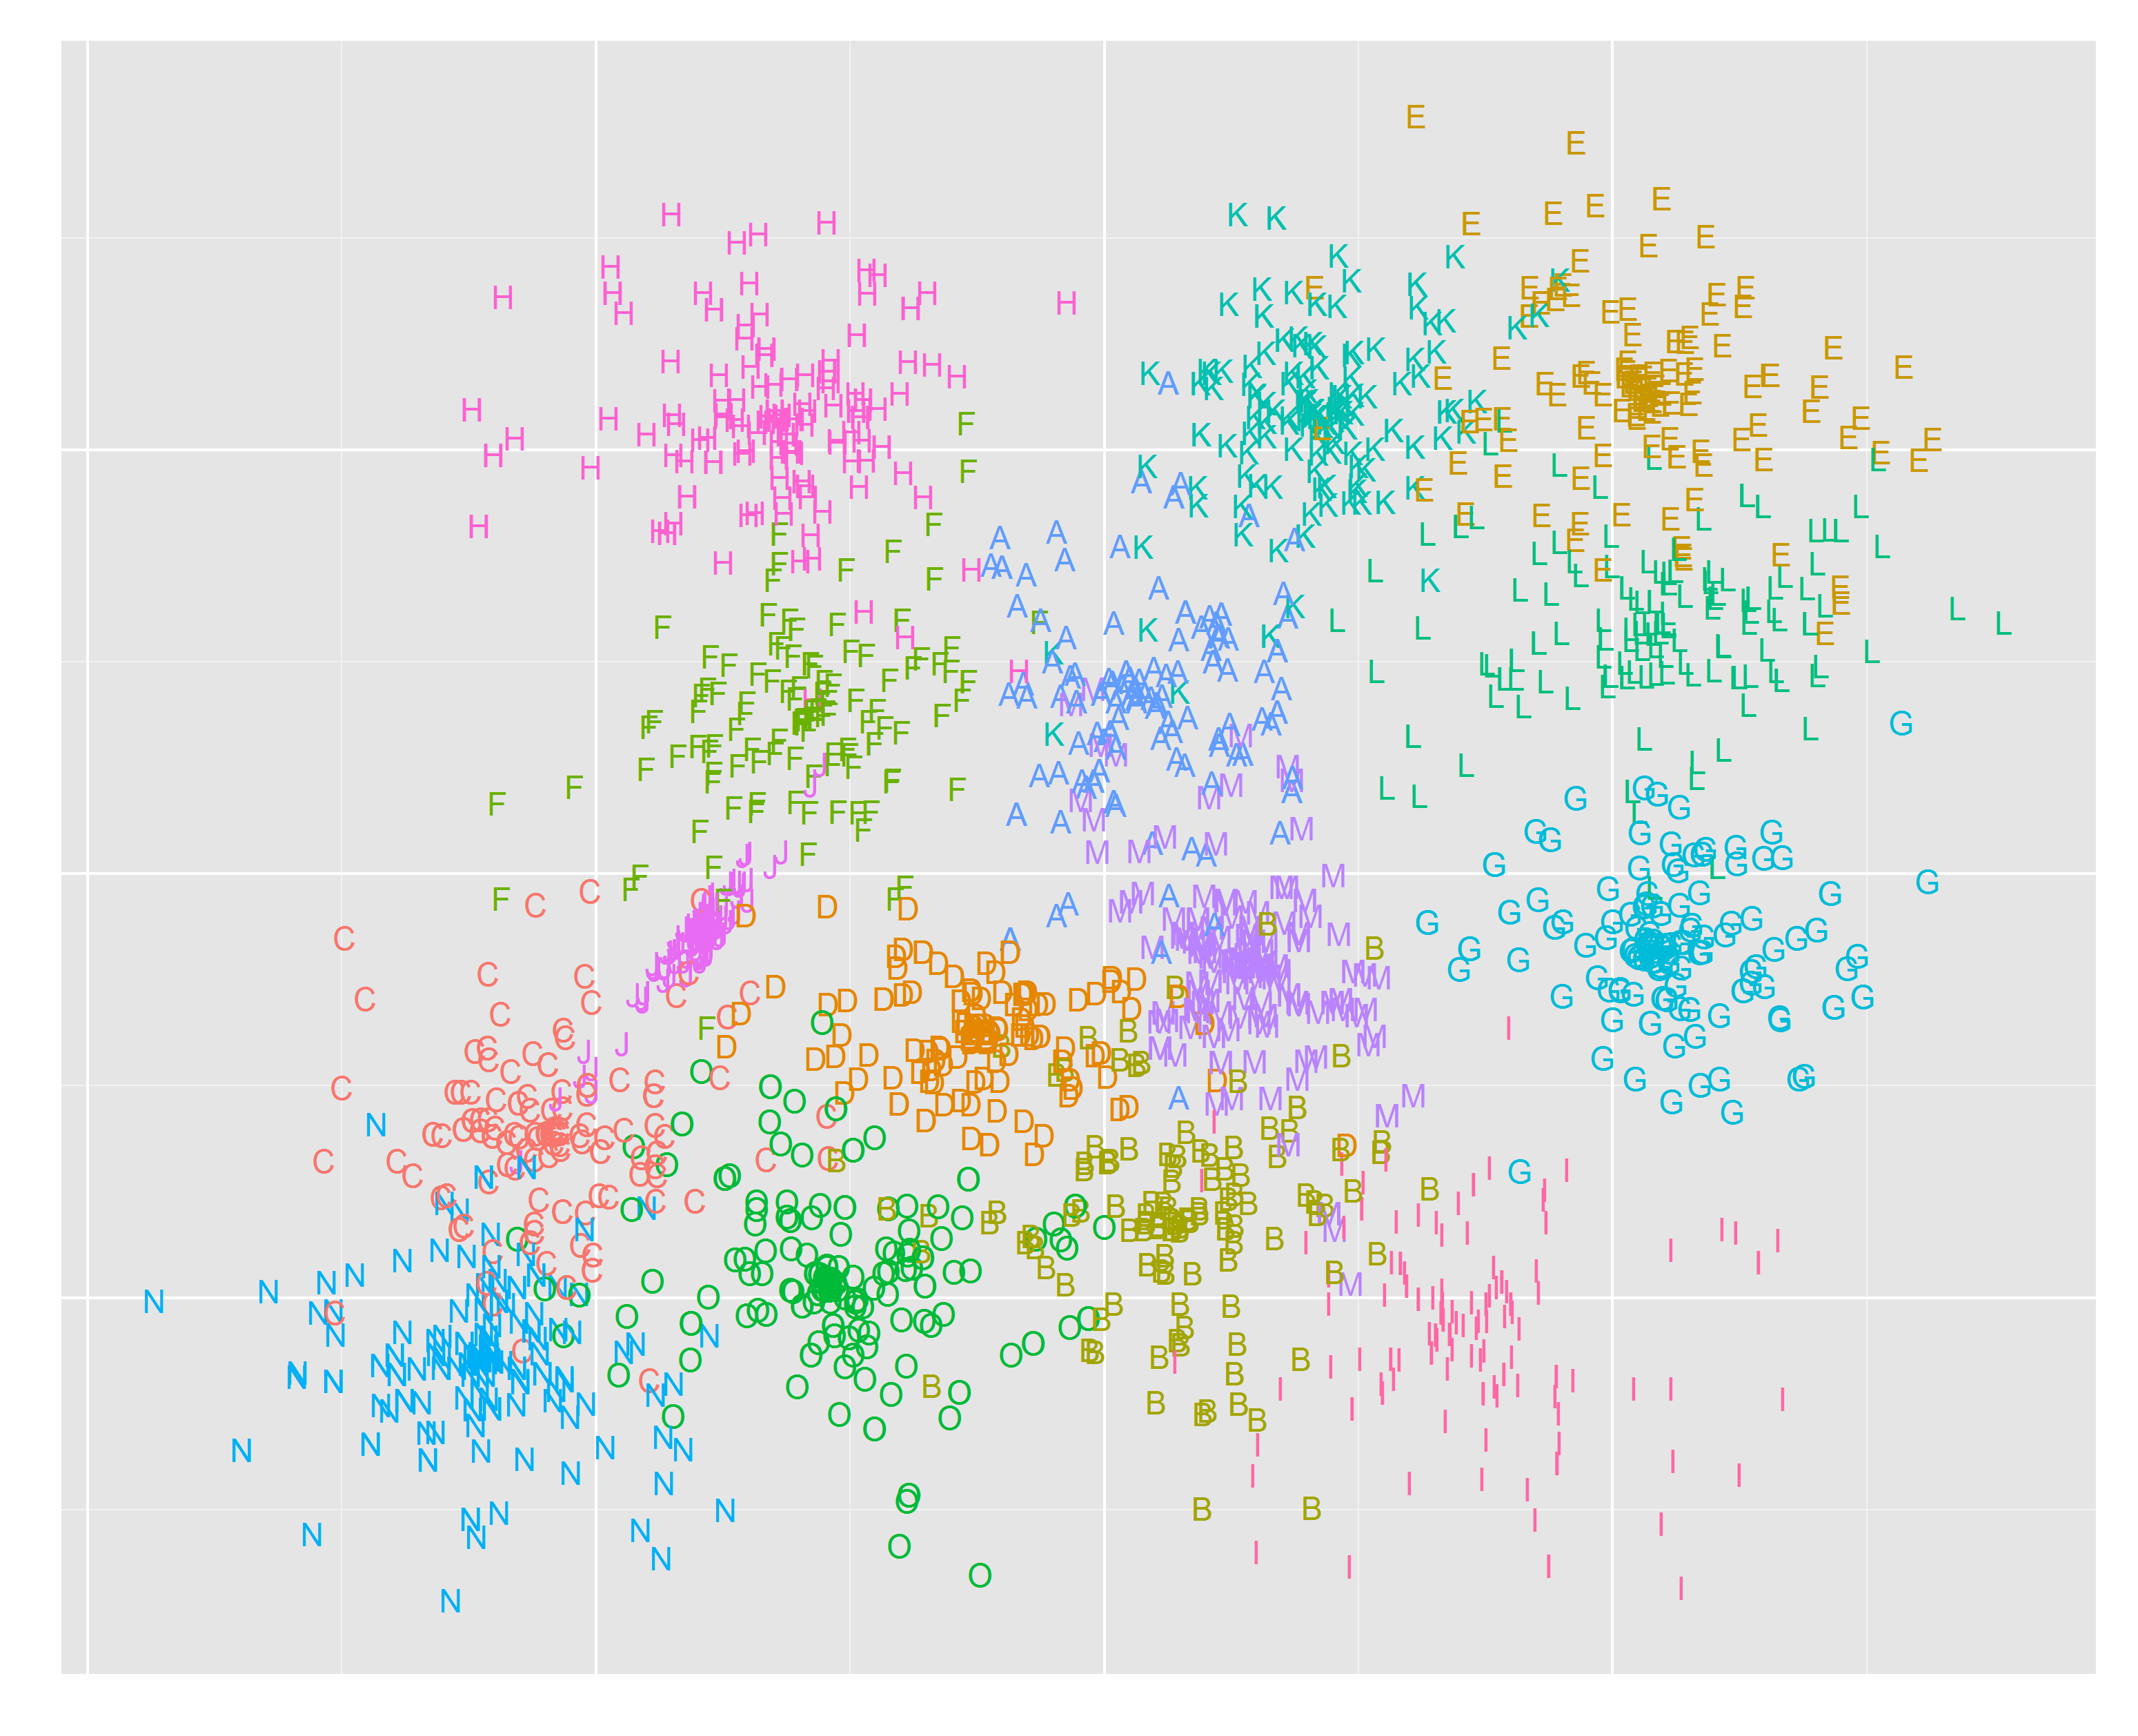
\includegraphics[width=.9\linewidth]{s_set/s_set_3_truth.png}
  \caption{S3}
 % \label{fig:sfig1}
\end{subfigure}%
\begin{subfigure}{.4\textwidth}
  \centering
  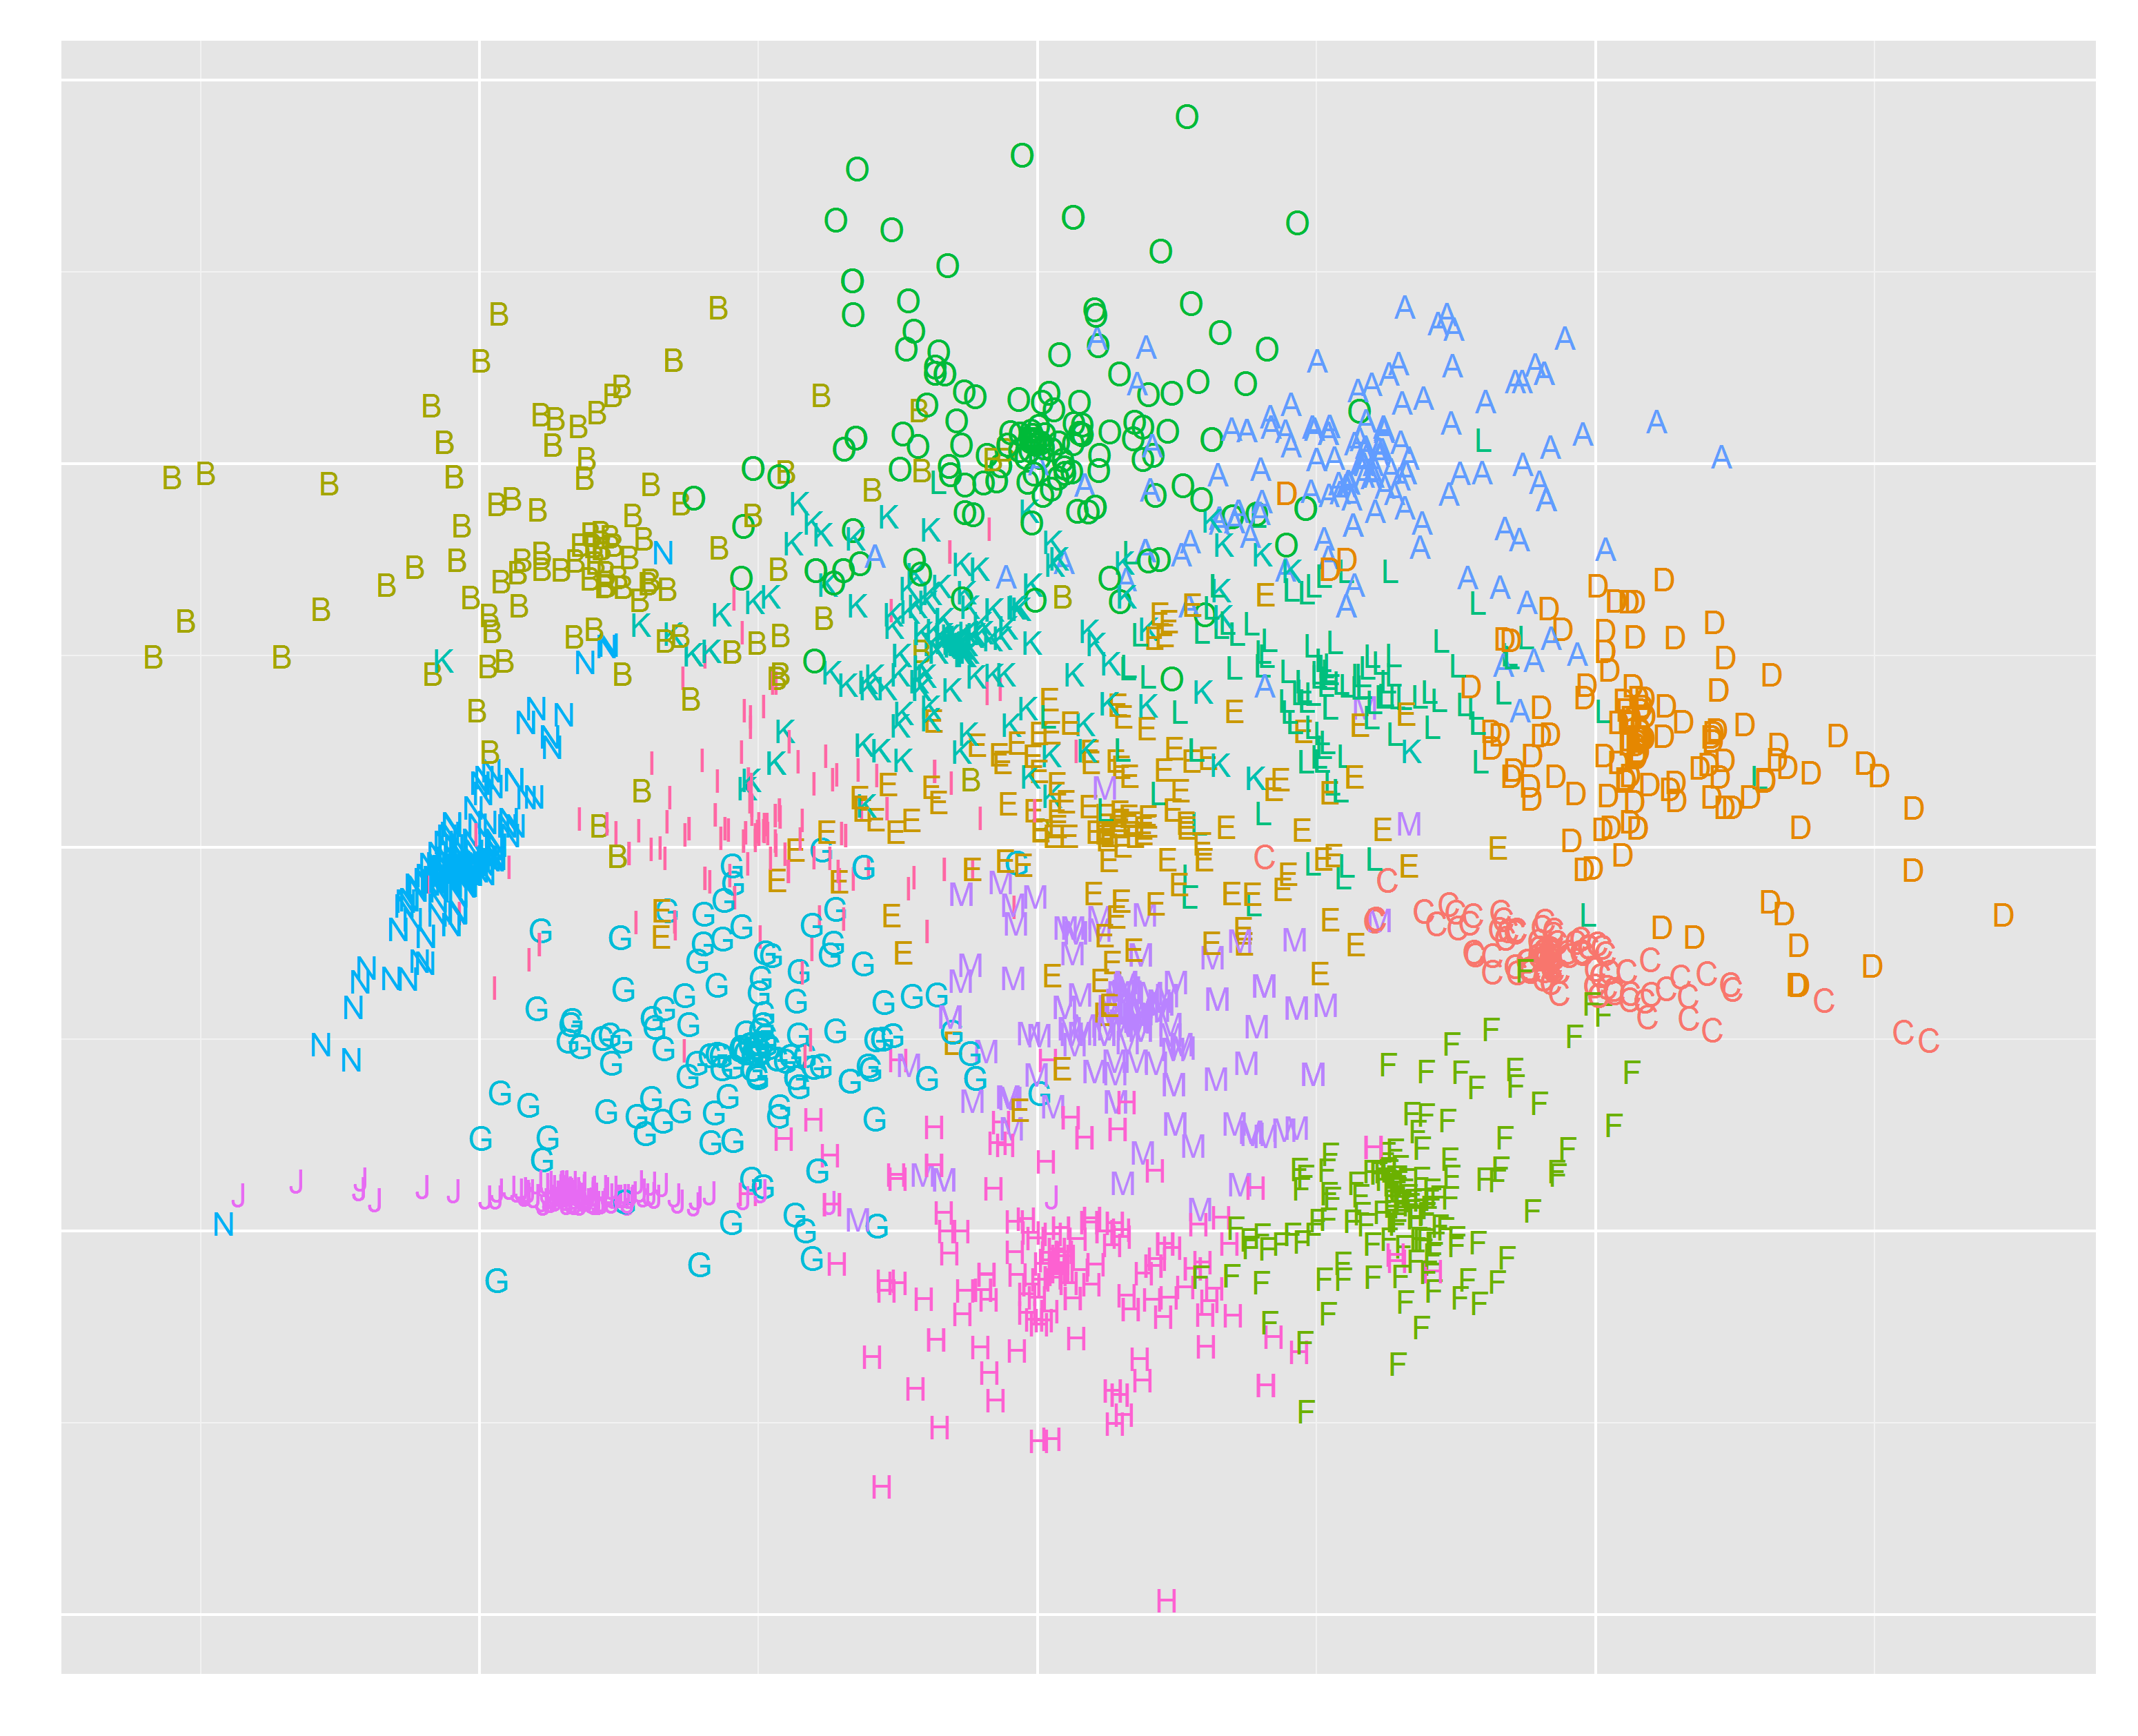
\includegraphics[width=.9\linewidth]{s_set/s_set_4_truth.png}
  \caption{S4}
%  \label{fig:sfig2}
\end{subfigure}
\caption{The S sets with true labels shown}
\label{fig:s_set_truth}
\end{figure}

Data set S1 should be the easiest to cluster as all 15 clusters are well fairly separated. The sets become increasingly more challenging and S4 can be difficult even for humans to separate correctly.  We treated each of these data sets as a data stream and used Spectral Clustream and Windowed Spectral Clustering to assign data points to clusters. Performance is evaluated in batch every $10^{th}$ time point. The results are shown in Figures \ref{fig:s_set_purity} and \ref{fig:s_set_vmeasure}. 

%%% Purity plots
\begin{figure}[H]
\begin{subfigure}{.45\textwidth}
  \centering
  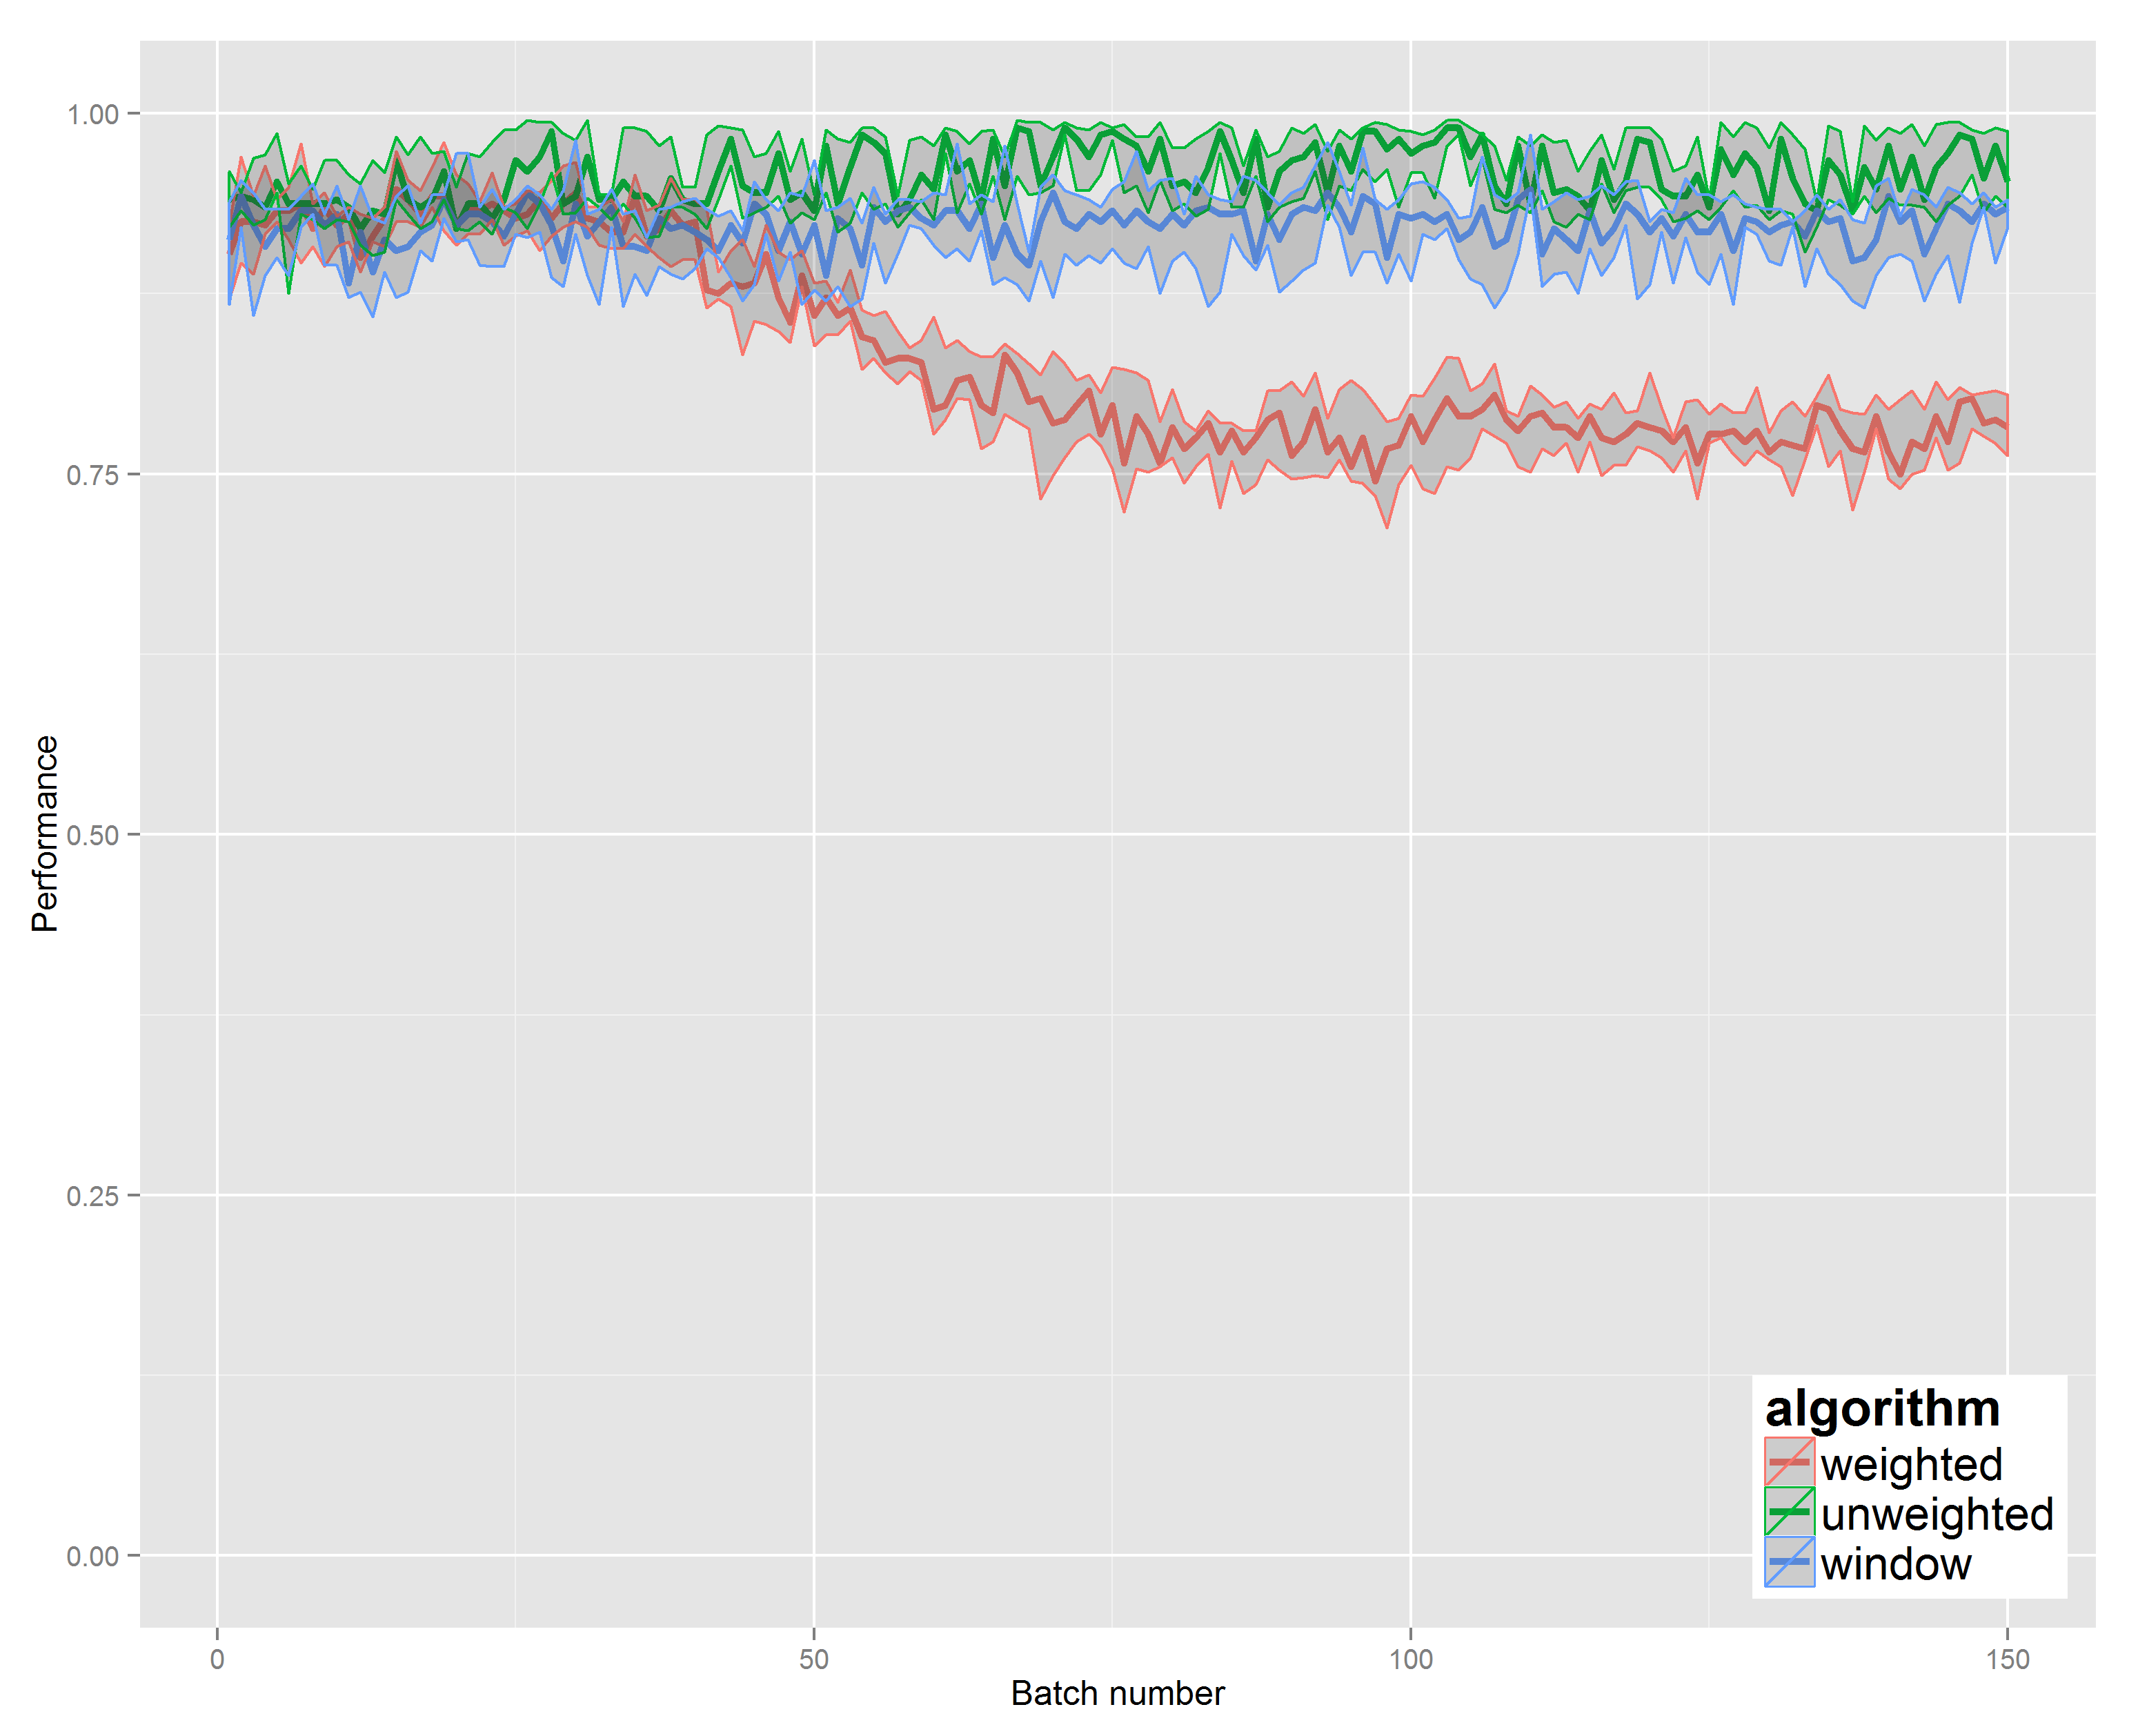
\includegraphics[width=.9\linewidth]{s_set/s_set_1_ci_one_size_purity.png}
  \caption{S1}
\end{subfigure}%
\begin{subfigure}{.45\textwidth}
  \centering
  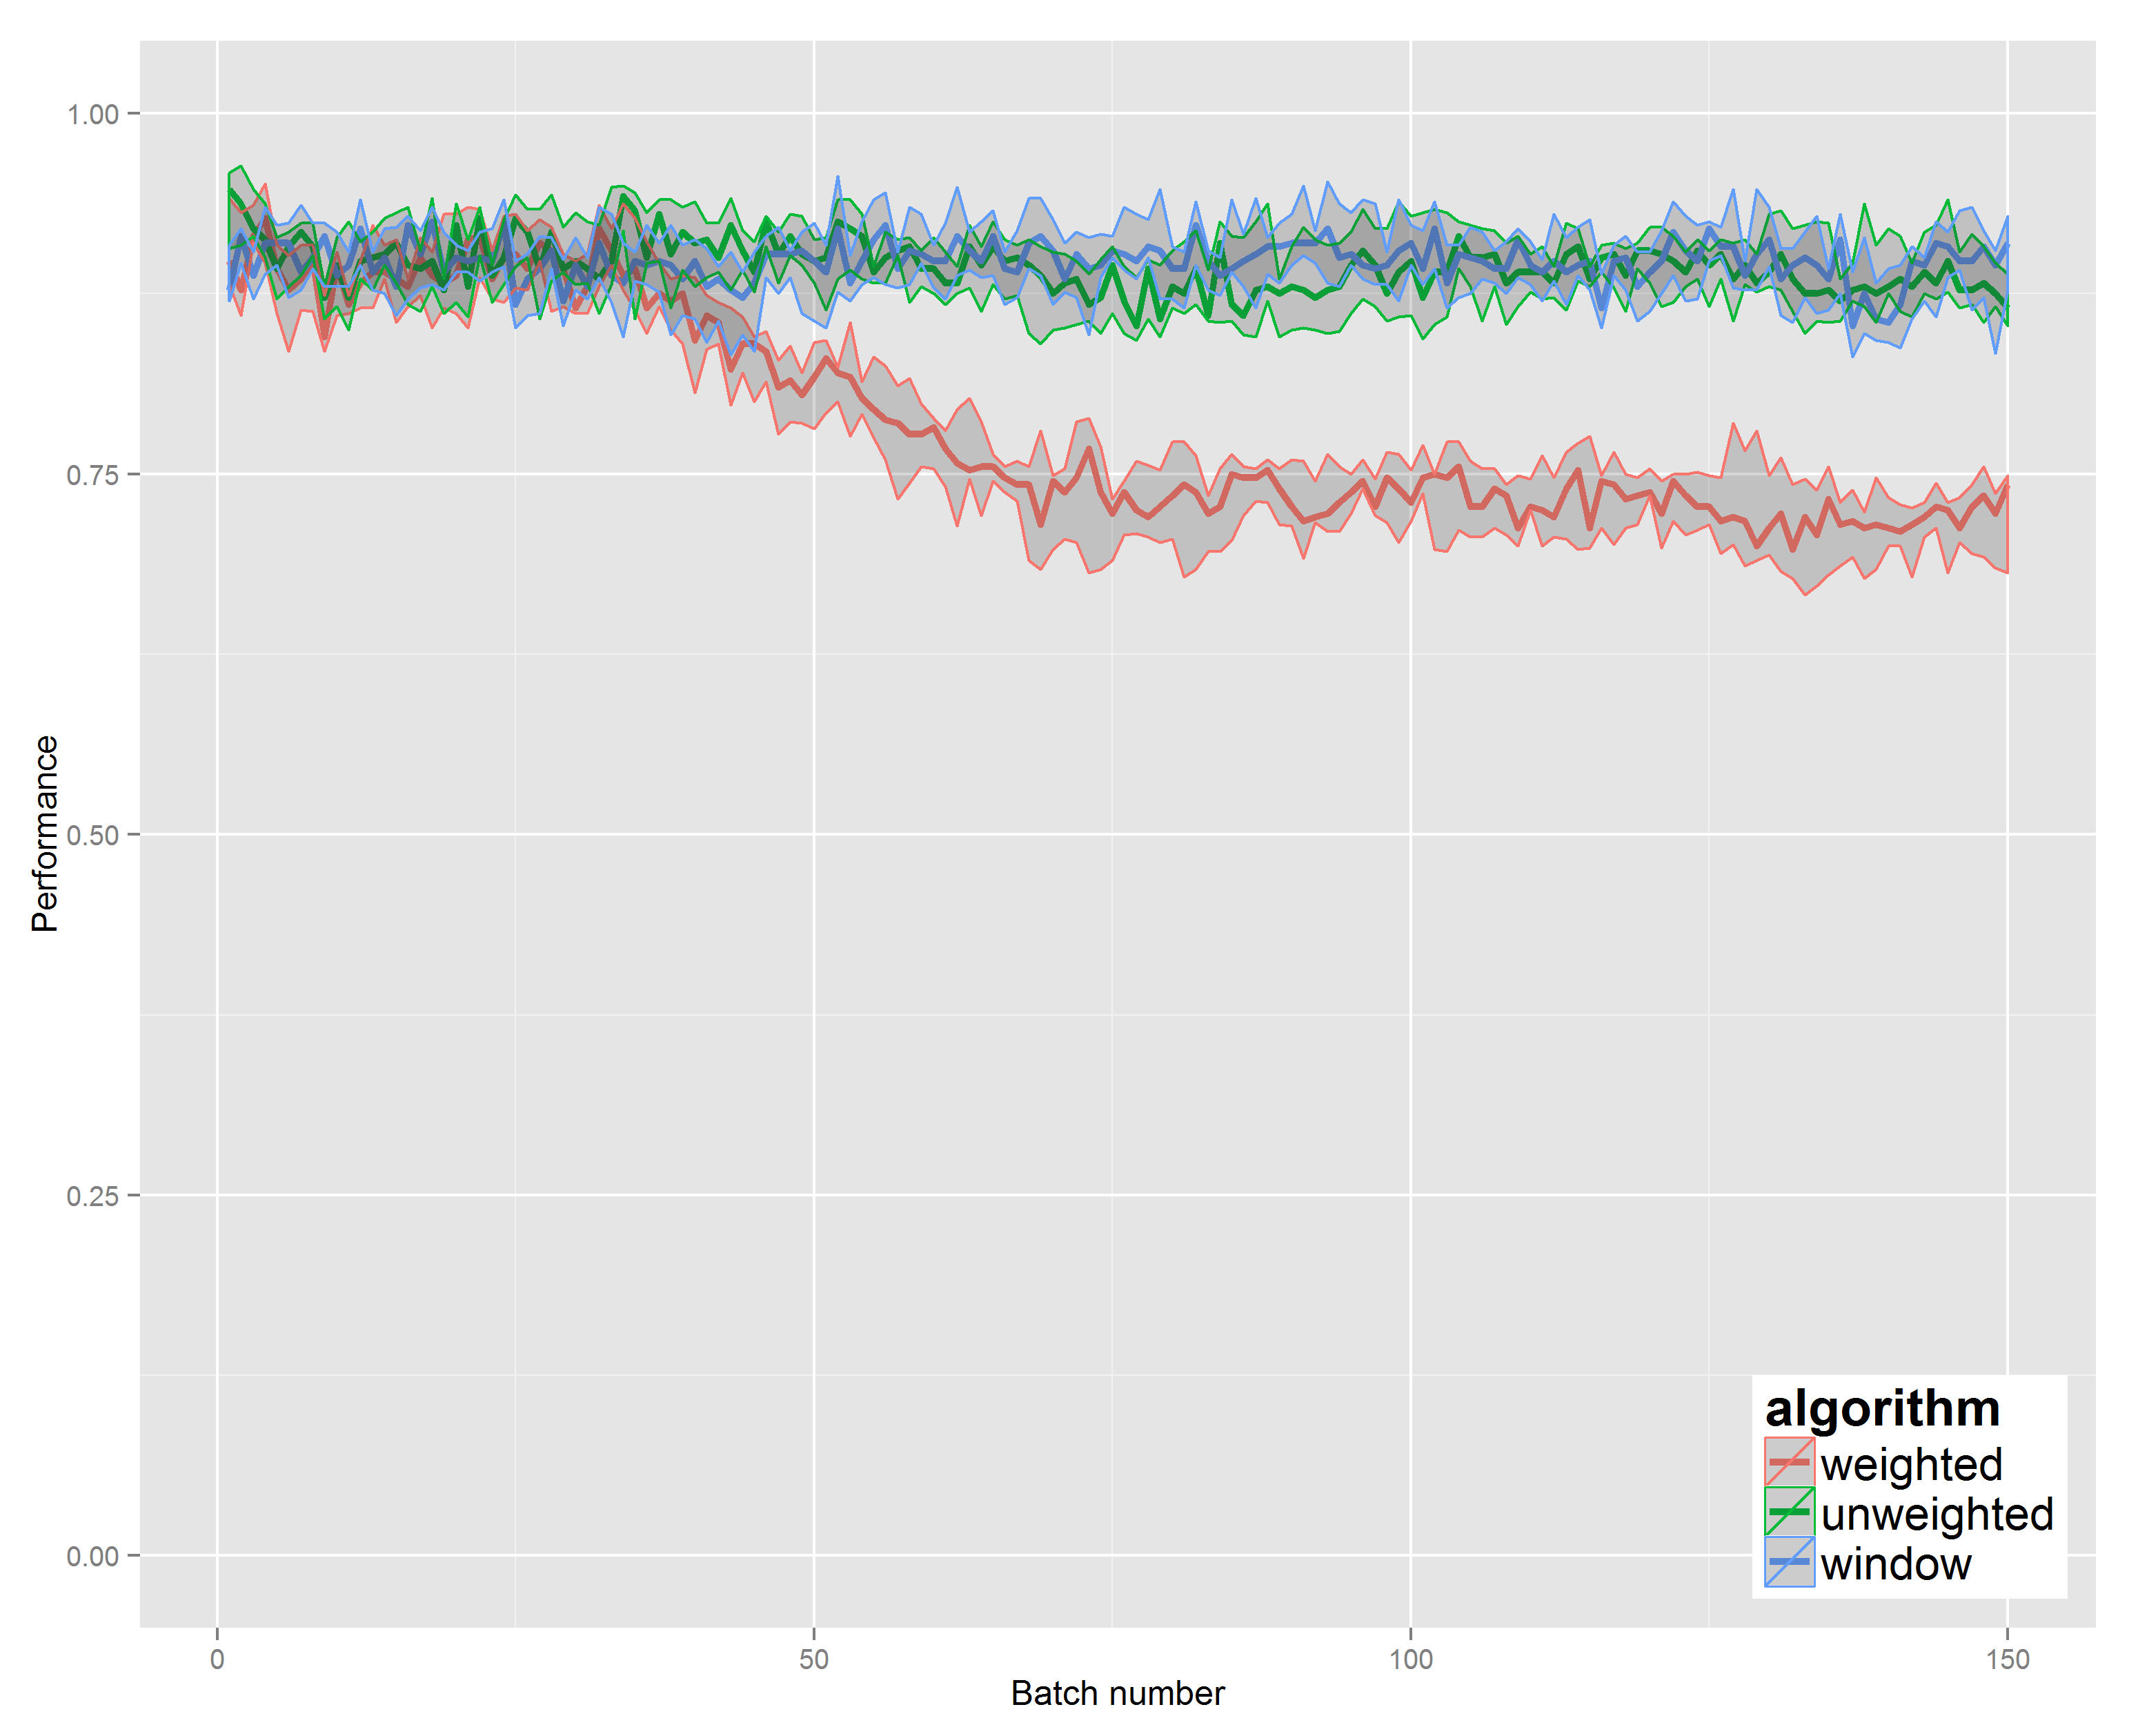
\includegraphics[width=.9\linewidth]{s_set/s_set_2_ci_one_size_purity.png}
  \caption{S2}
\end{subfigure}
\begin{subfigure}{.45\textwidth}
  \centering
  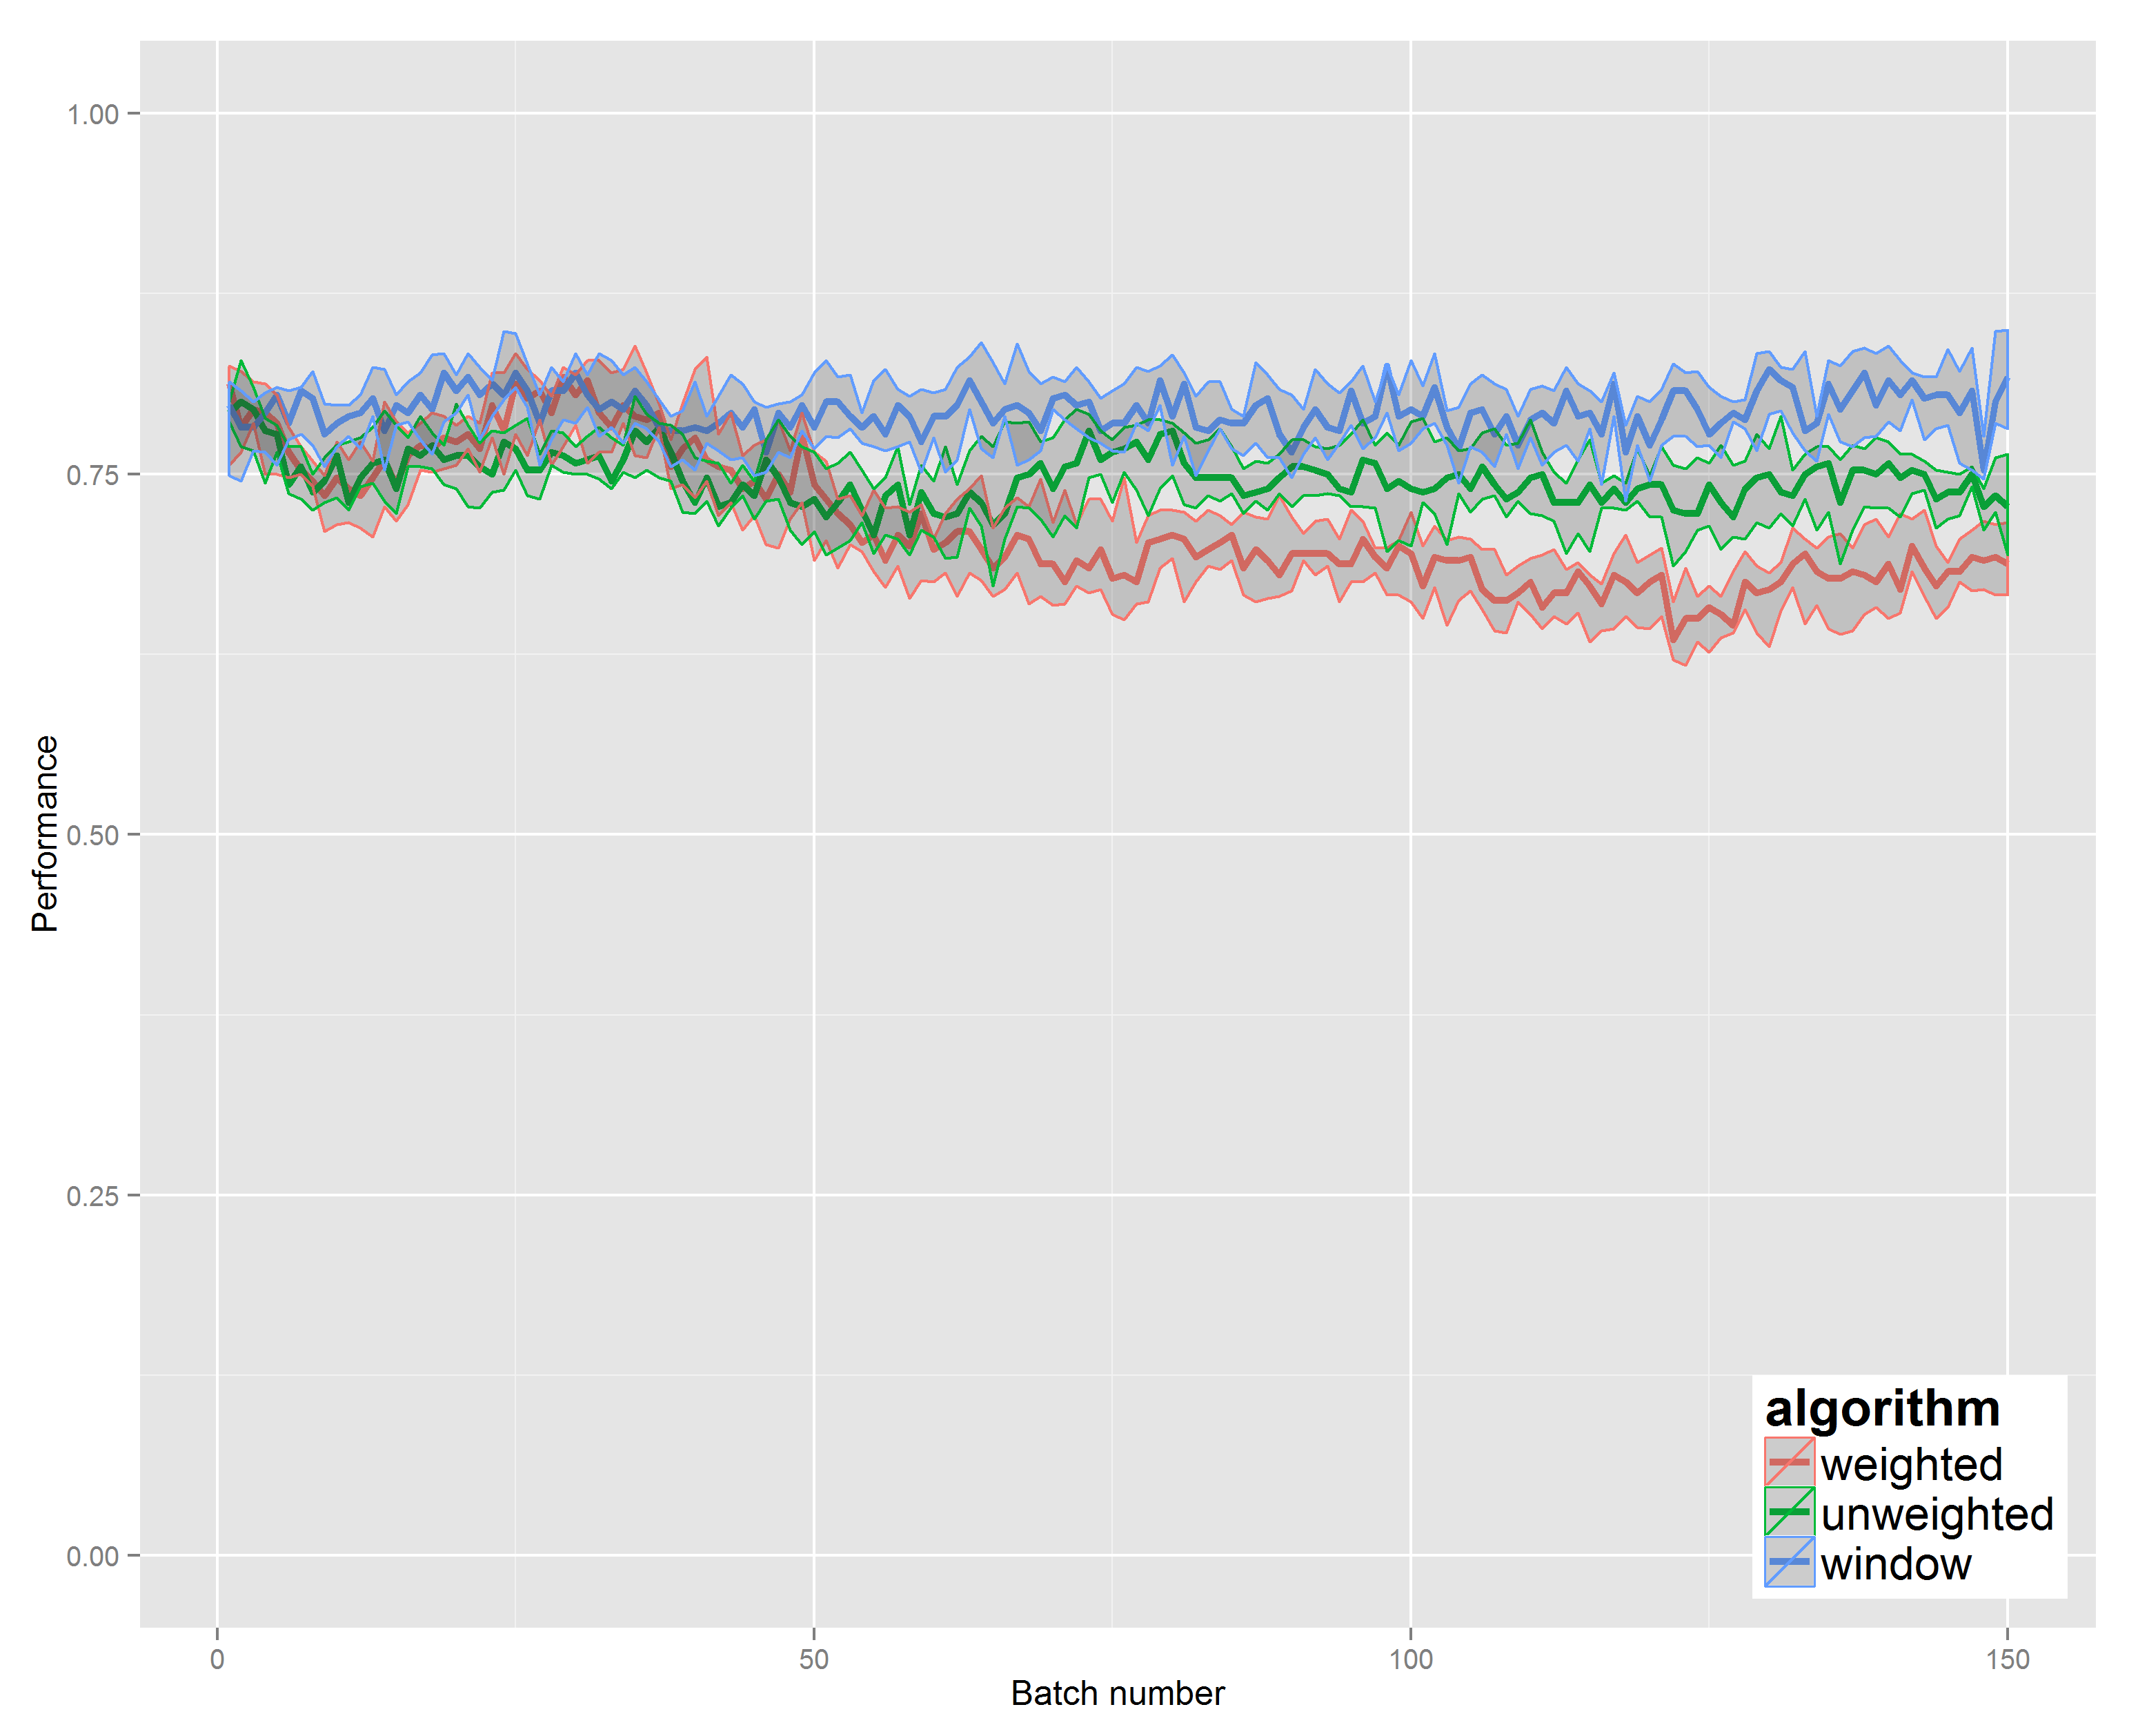
\includegraphics[width=.9\linewidth]{s_set/s_set_3_ci_one_size_purity.png}
  \caption{S3}
\end{subfigure}%
\begin{subfigure}{.45\textwidth}
  \centering
  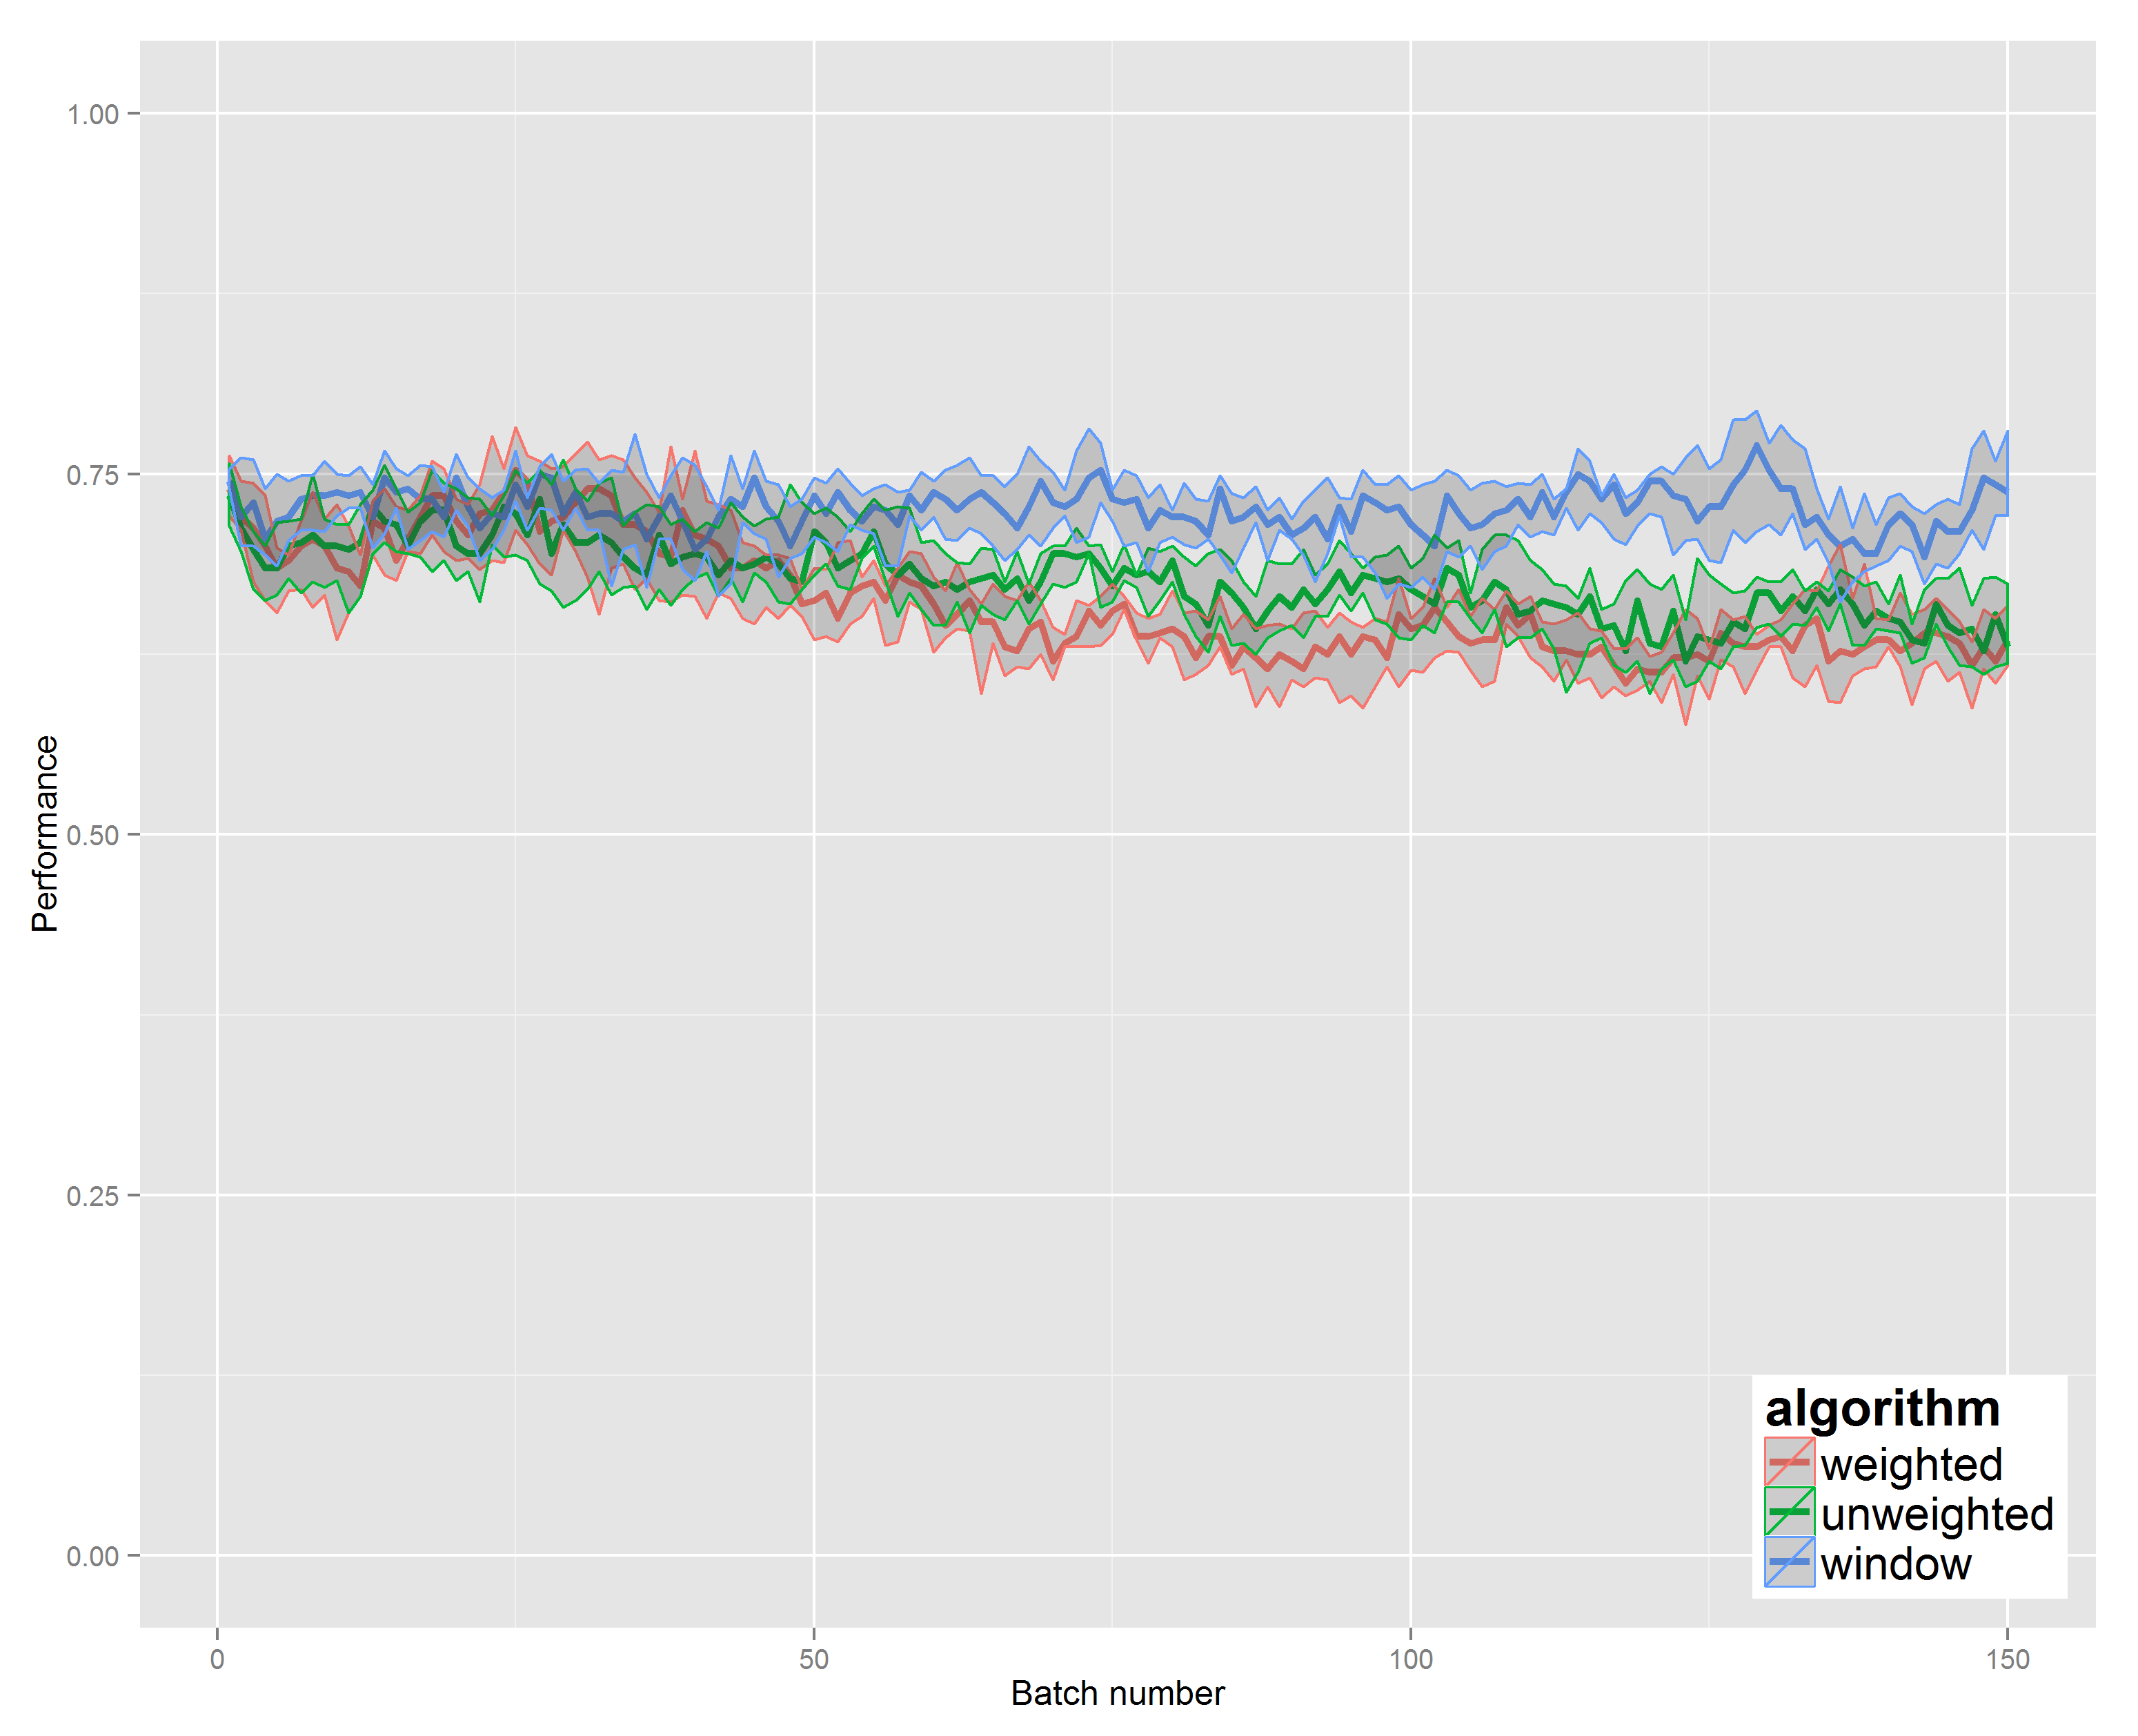
\includegraphics[width=.9\linewidth]{s_set/s_set_4_ci_one_size_purity.png}
  \caption{S4}
\end{subfigure}
\caption{Purity for the S data sets.}
\label{fig:s_set_purity}
\end{figure}

Figure \ref{fig:s_set_purity} plots the performance in terms of purity on the y-axis and the batch number is given on the x-axis. The average performance for each algorithm over the multiple runs is given by the thick solid lines and the shaded area depicts the inter-quartile range.  Figure \ref{fig:s_set_vmeasure} shows the performance in terms of V-measure.  Both figures show the algorithm performance at each batch step, meaning that we can see how performance changes as the data stream progresses. However, these data sets are stationary in distribution and therefore we would not expect to see algorithm performance vary dramatically with time. 

Both unweighted Spectral Clustream (green) and windowed Spectral  Clustering (blue) perform similarly for all sets.  They both perform well on set S1 and set S2 but they struggle with the more challenging sets S3 and S4.   The Weighted Spectral Clustream (red) initially starts with performance on par with the competing algorithms, but quickly drops to poor performance and does not recover as the stream progresses. Given that the underlying distributions for the S sets are stationary, this behaviour is unusual.

%%%% V-measure plots
\begin{figure}[H]
\begin{subfigure}{.45\textwidth}
  \centering
  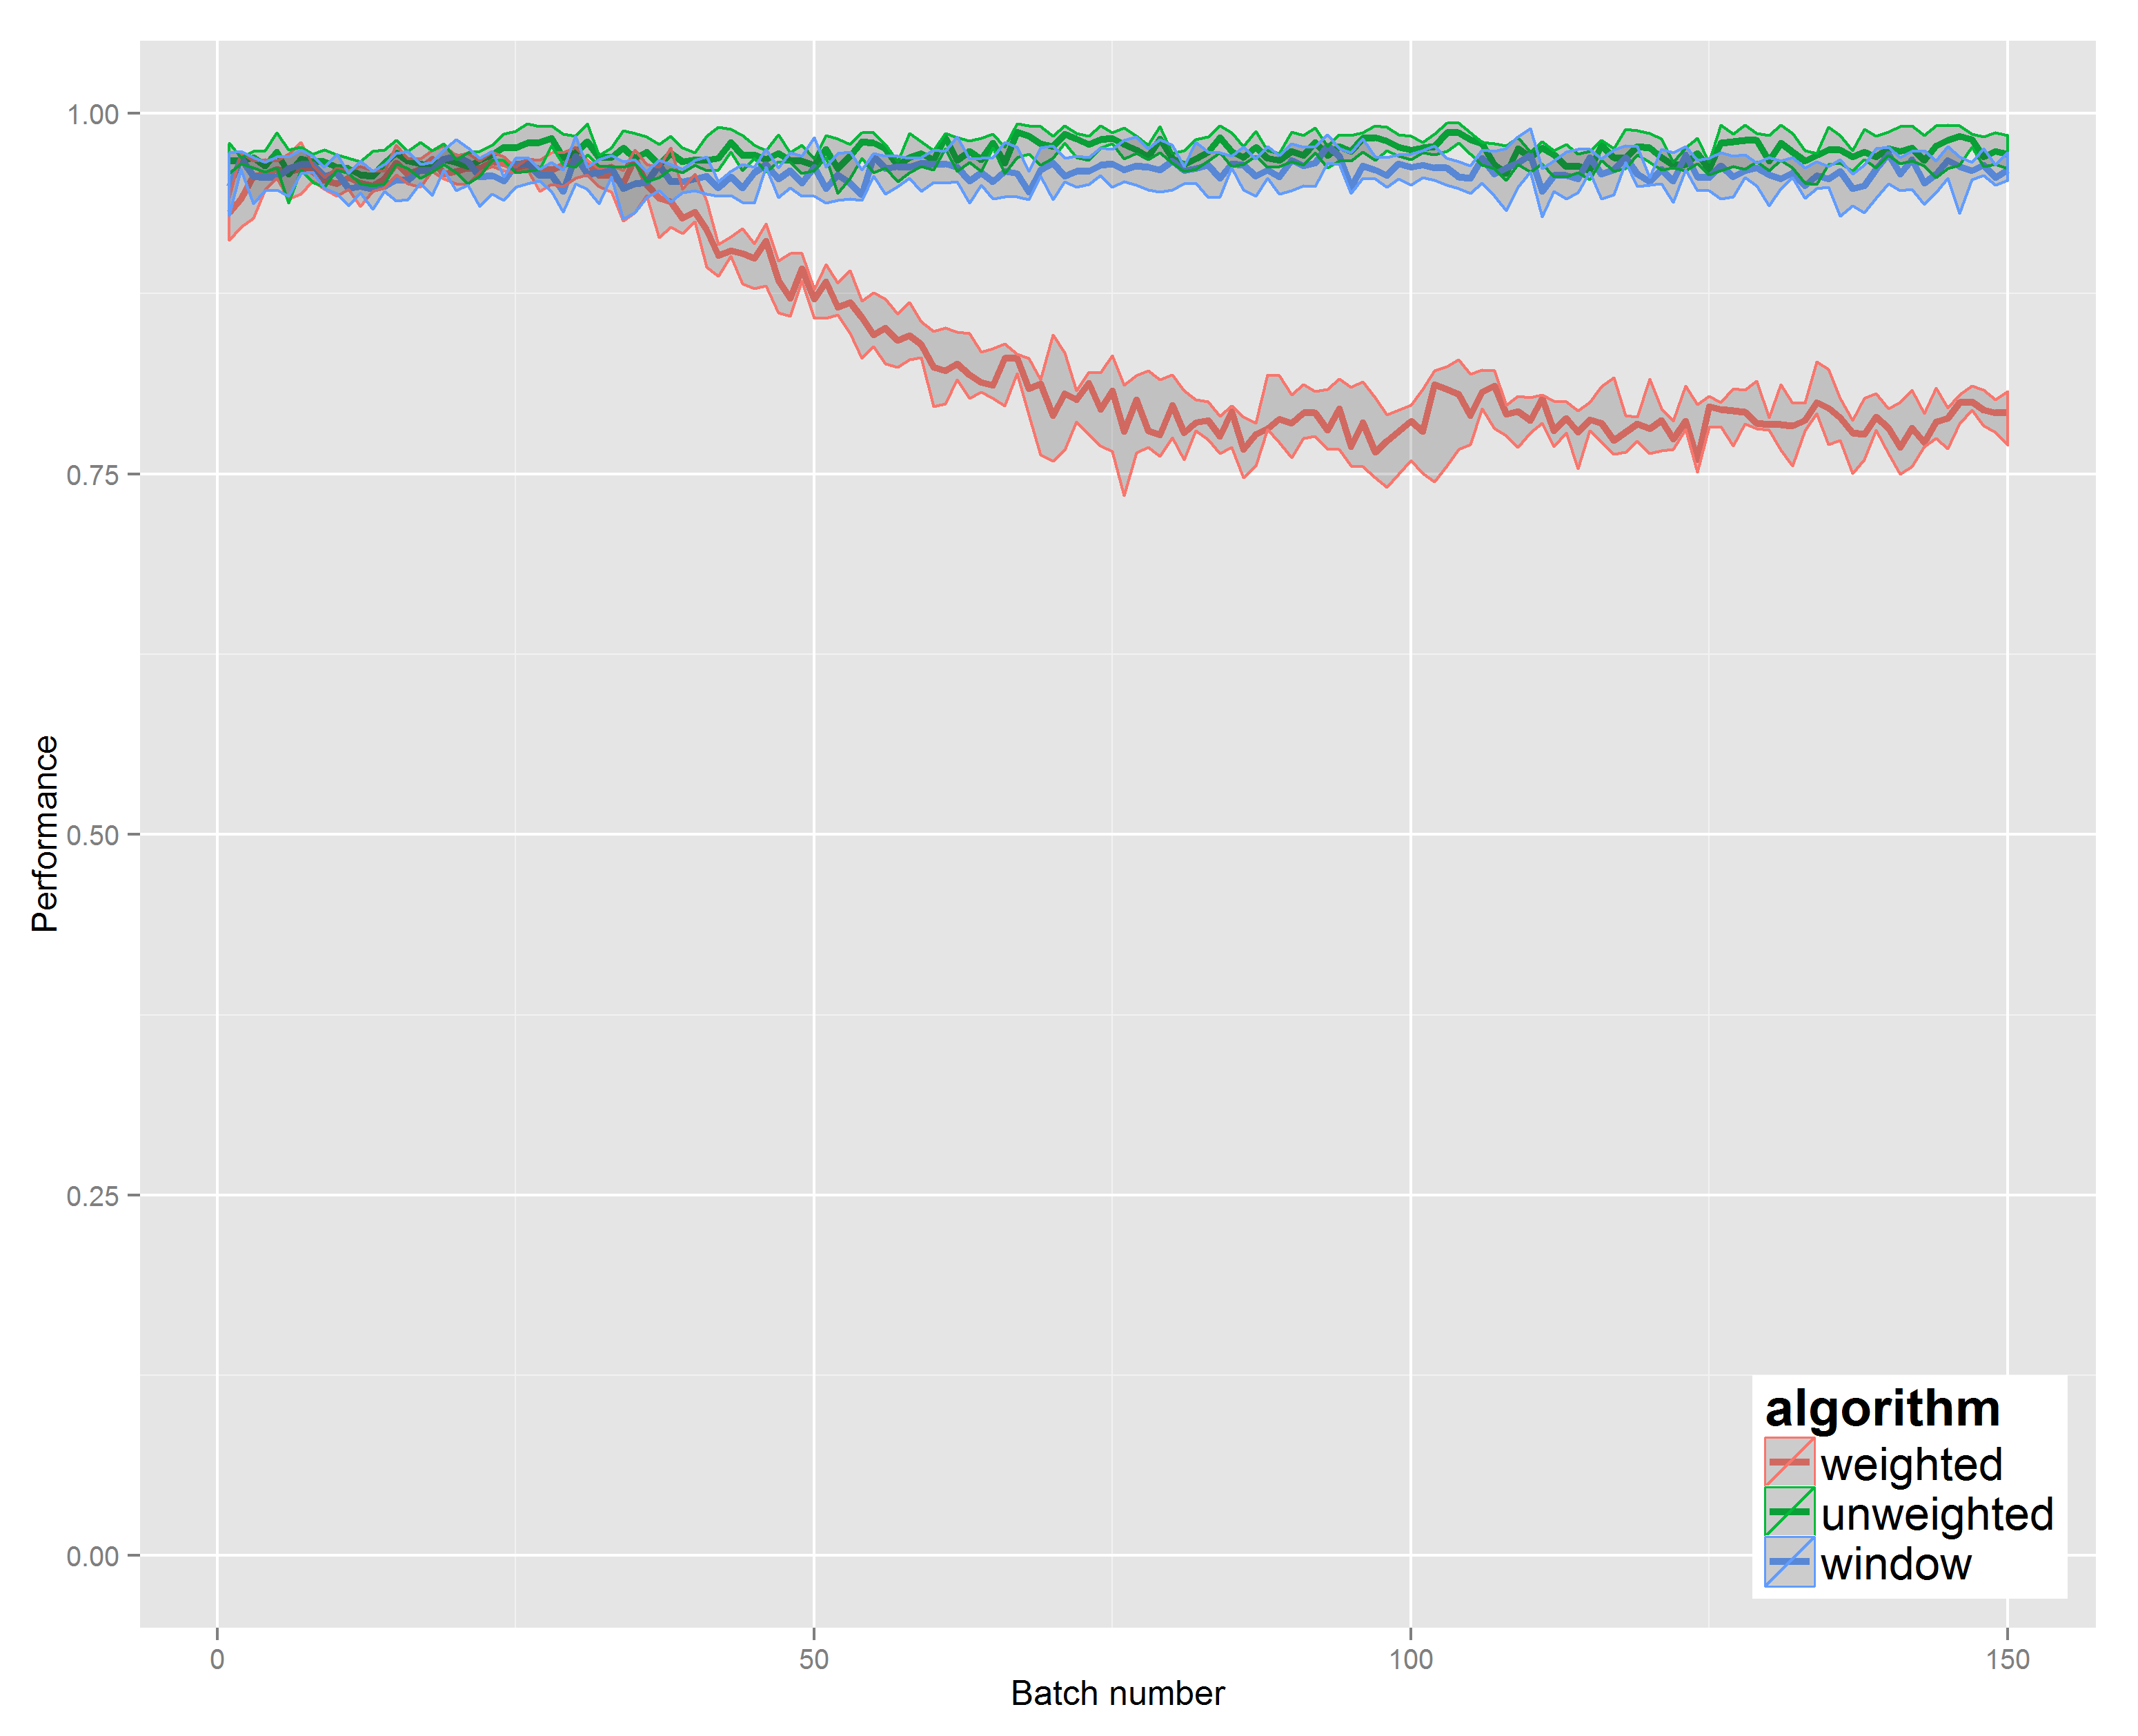
\includegraphics[width=.9\linewidth]{s_set/s_set_1_ci_one_size_vmeasure.png}
  \caption{S1}
\end{subfigure}%
\begin{subfigure}{.45\textwidth}
  \centering
  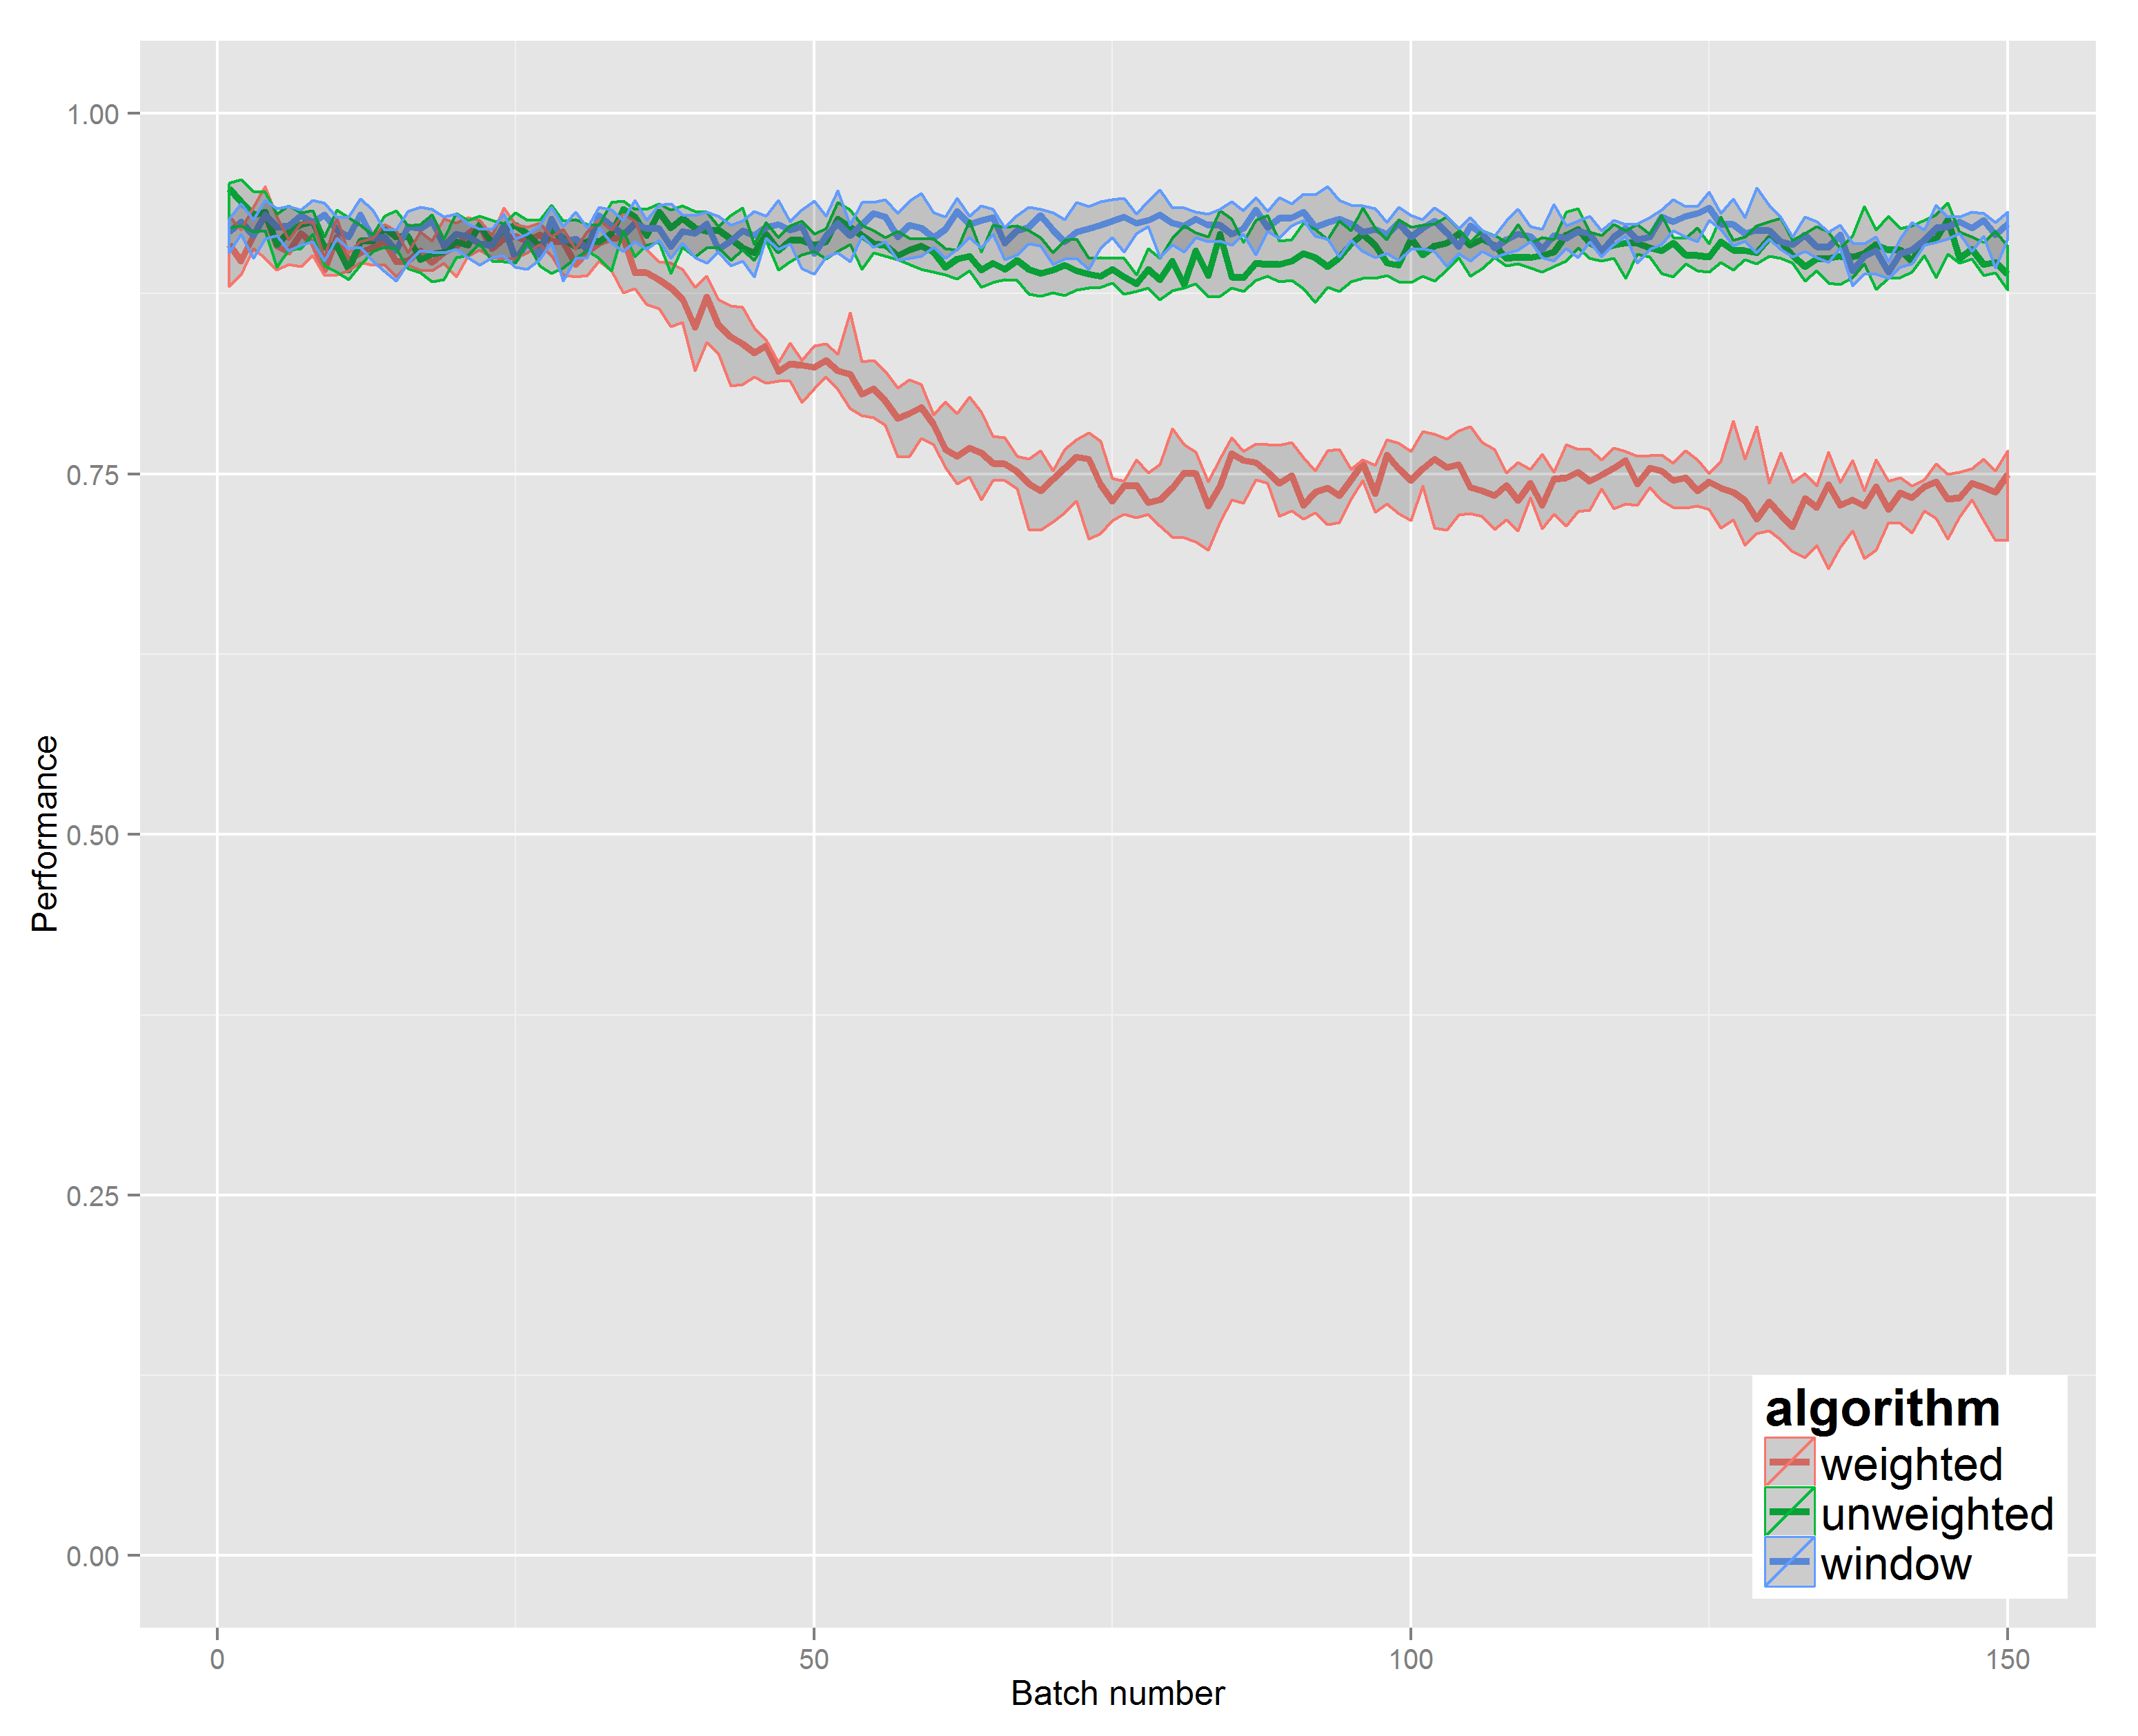
\includegraphics[width=.9\linewidth]{s_set/s_set_2_ci_one_size_vmeasure.png}
  \caption{S2}
\end{subfigure}
\begin{subfigure}{.45\textwidth}
  \centering
  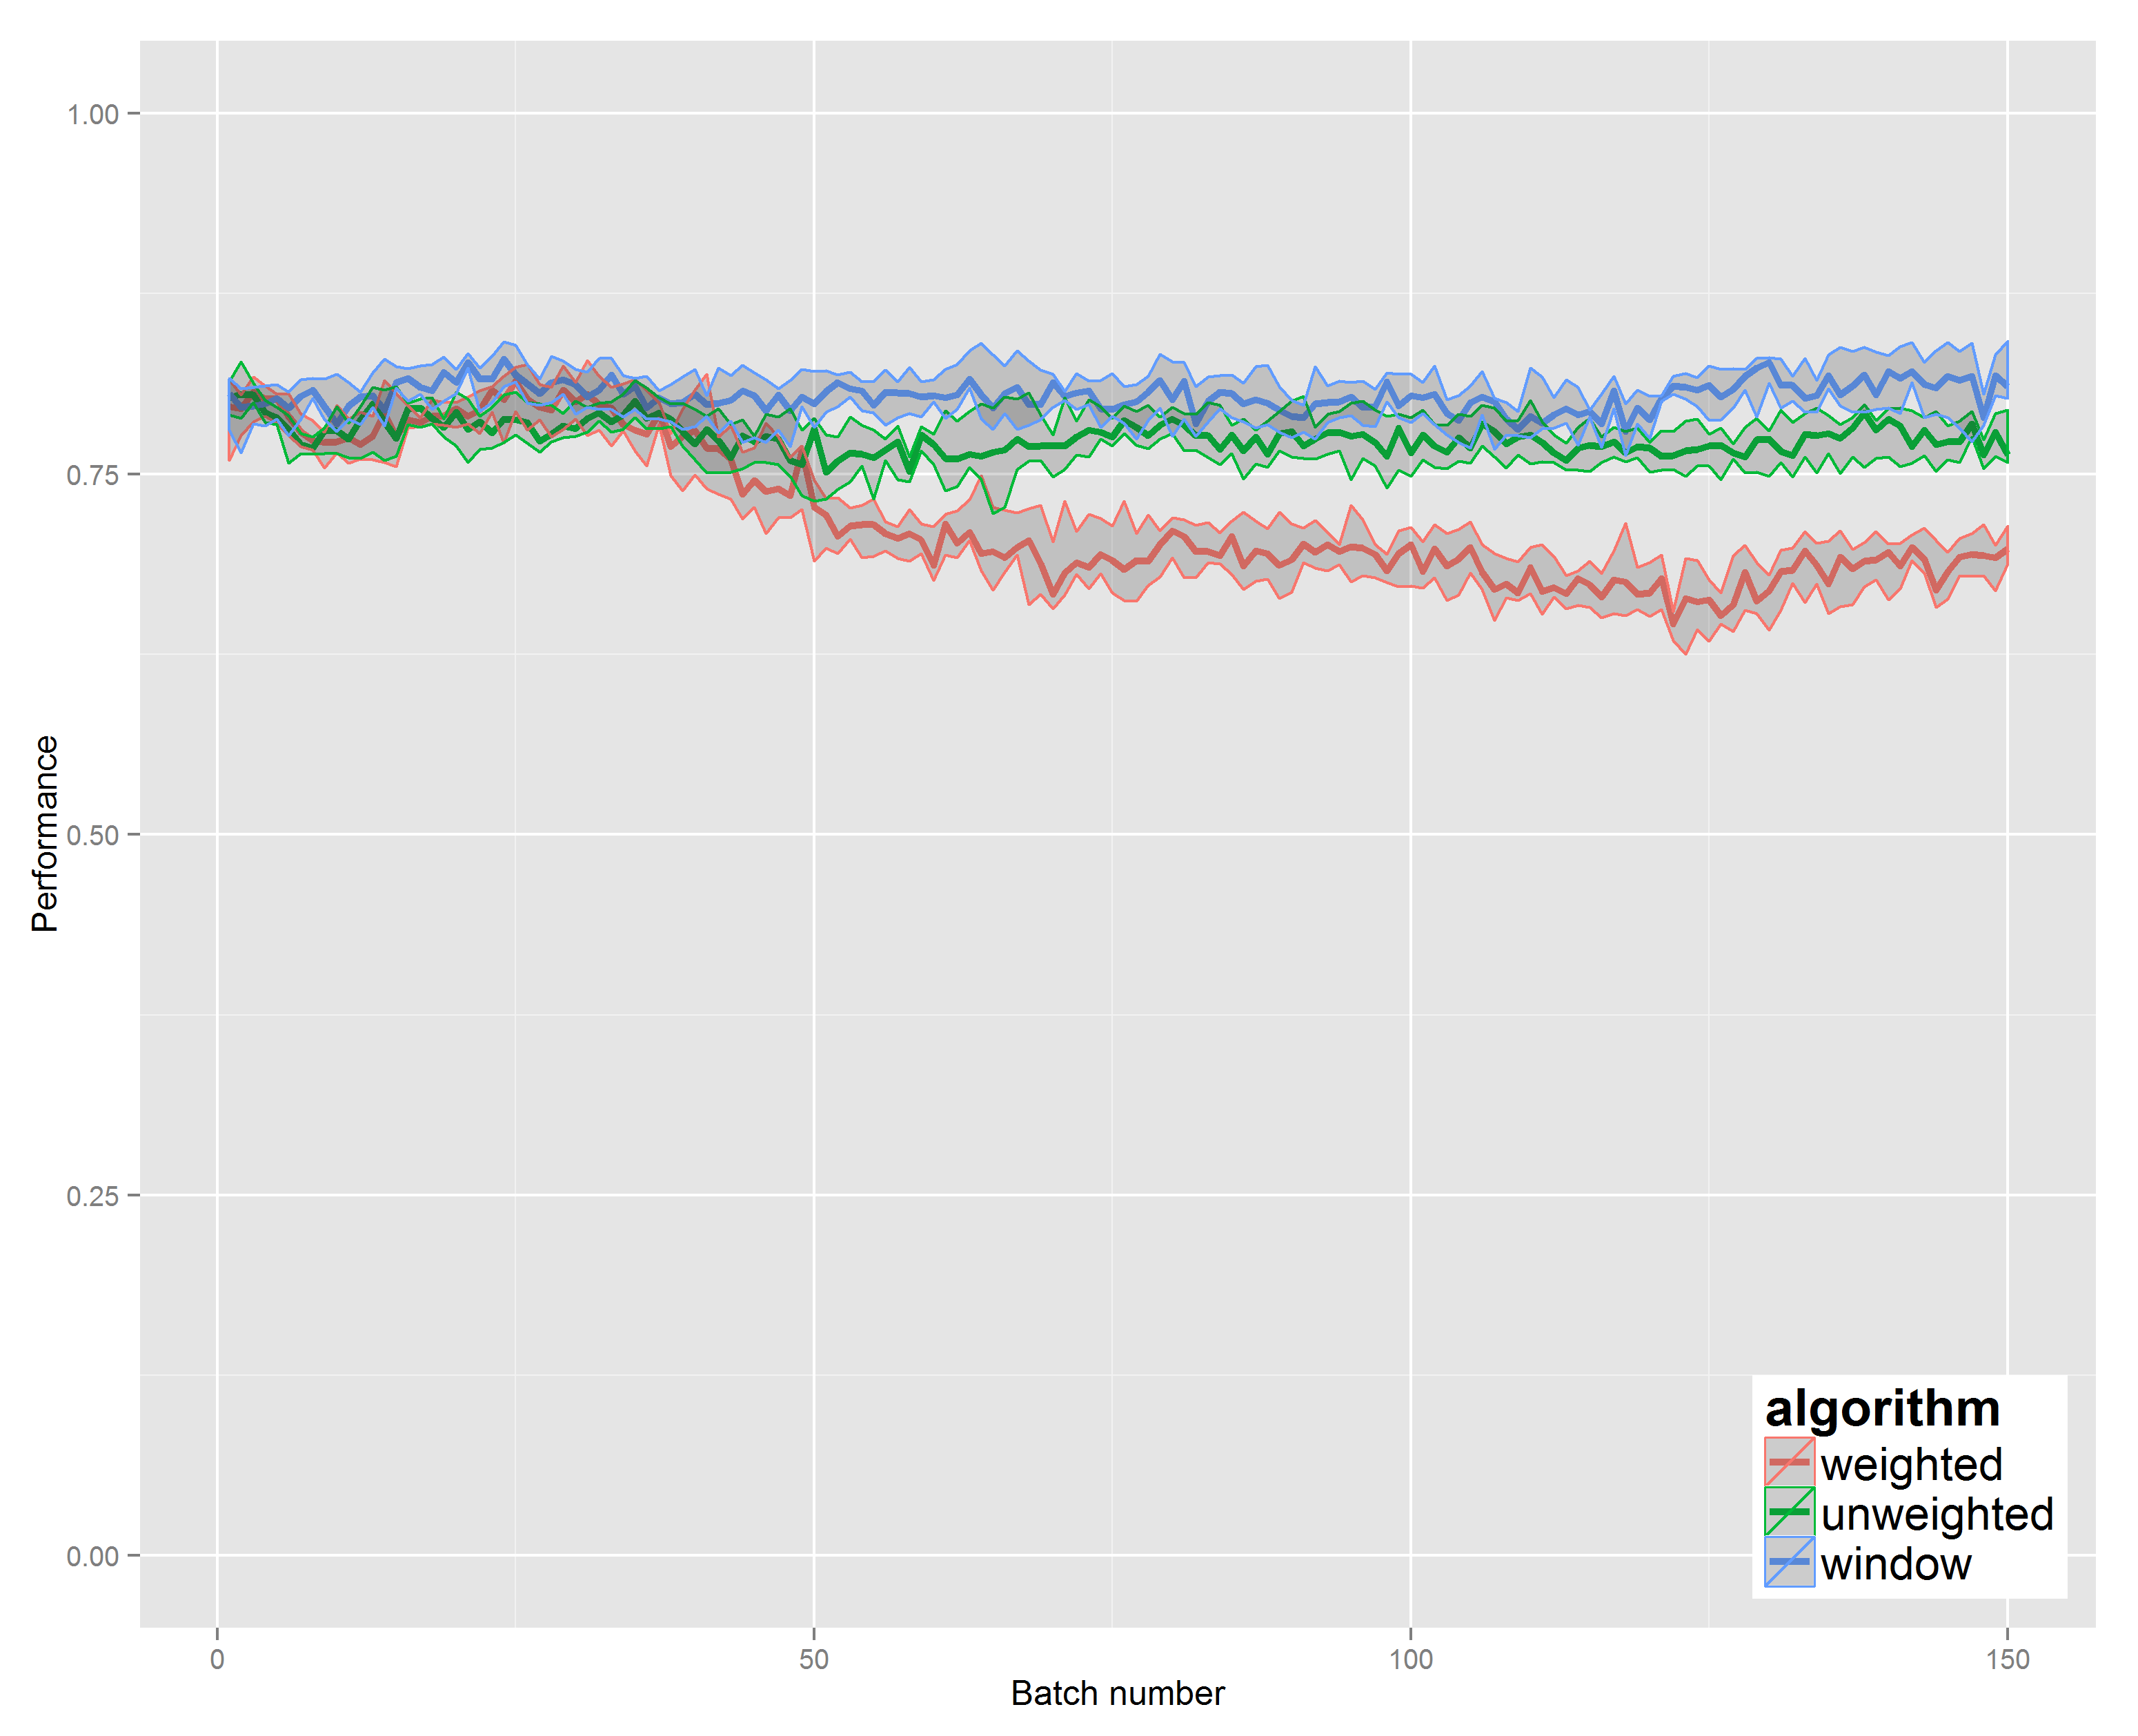
\includegraphics[width=.9\linewidth]{s_set/s_set_3_ci_one_size_vmeasure.png}
  \caption{S3}
\end{subfigure}%
\begin{subfigure}{.45\textwidth}
  \centering
  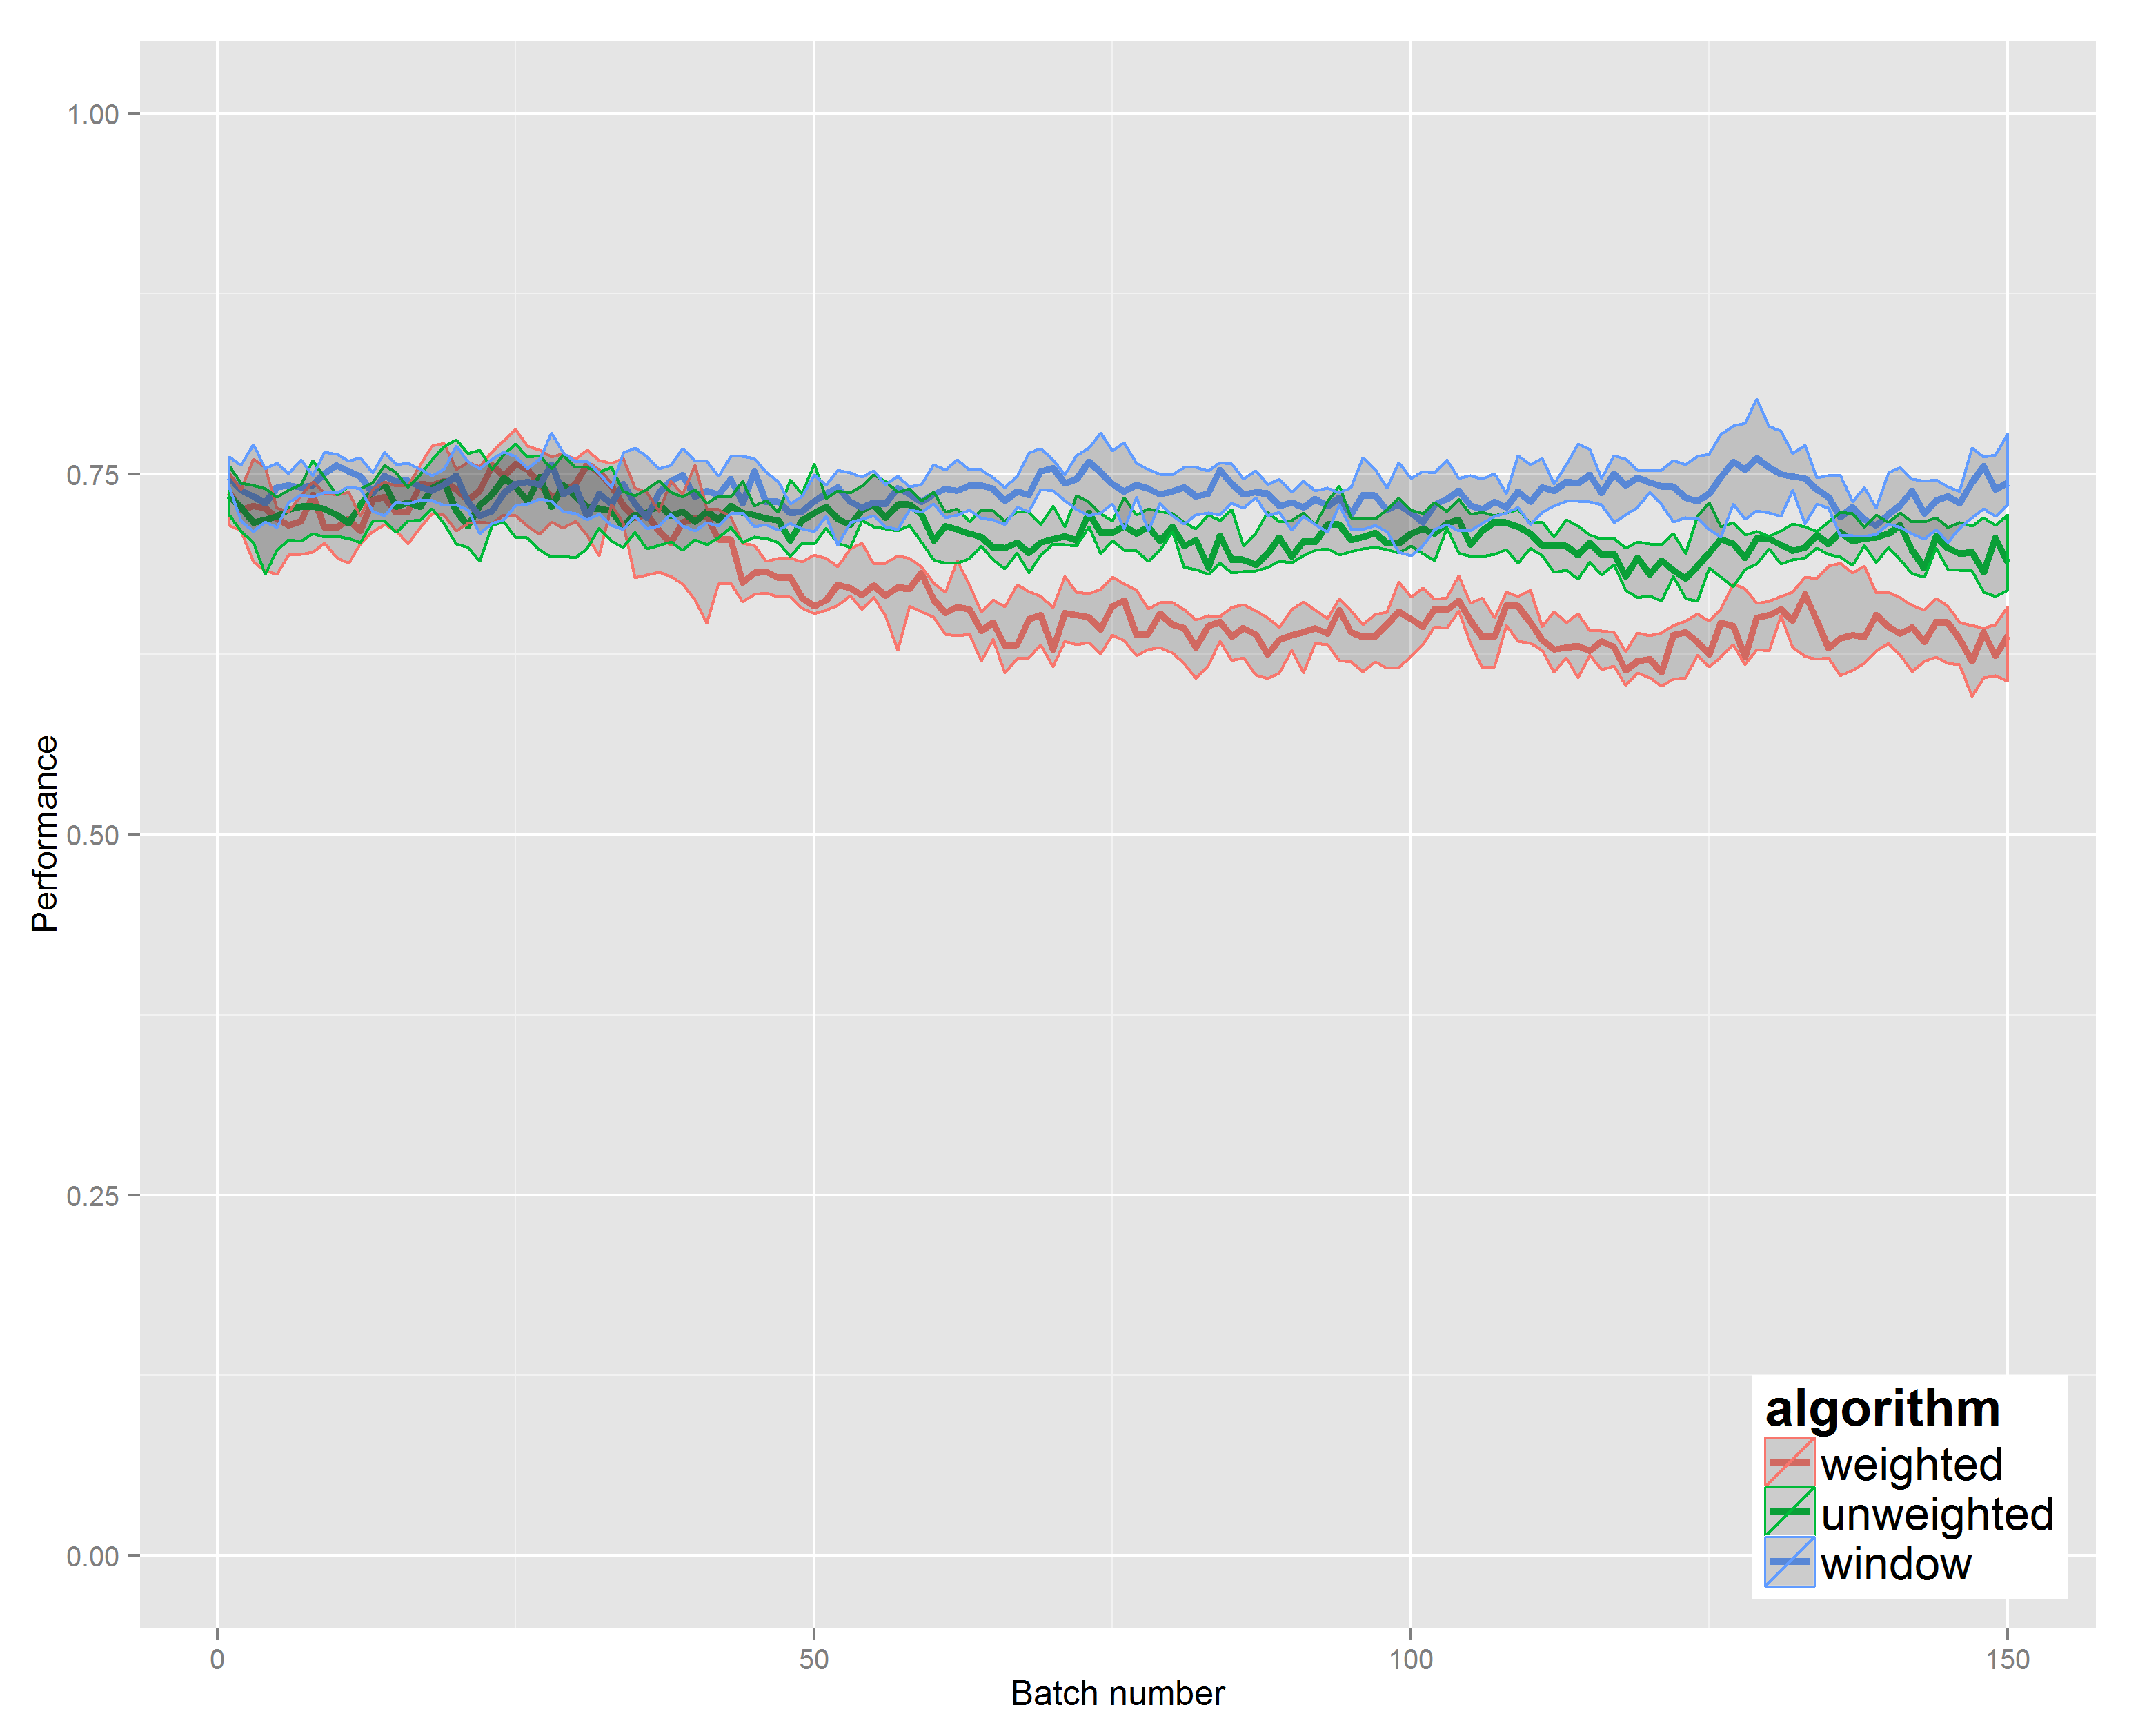
\includegraphics[width=.9\linewidth]{s_set/s_set_4_ci_one_size_vmeasure.png}
  \caption{S4}
\end{subfigure}
\caption{V-measure for the S data sets.}
\label{fig:s_set_vmeasure}
\end{figure}

In order to discover why Weighted Spectral Clustream is performing poorly, lets look at the micro-clusters more closely. Figure \ref{fig:weighted_issues} shows a snapshot of the Weighted Spectral Clustream algorithm on the S1 data set in the middle of the stream. The grey points are the data points observed so far, the location of the letters represent micro-cluster centres which are labelled with the results of the Weighted Spectral Clustering. This is not a good clustering of the data.  We can see that one cluster (letter N) is dominating and many of the outliers of the other clusters have been represented by the N cluster label. This implies that the affinities between the micro-cluster centres on the outskirts of the cluster C are more similar to the outliers of other clusters (such as cluster I) than to the micro-cluster centres at C. This behaviour is very odd and implies that there might be an issue with the  affinity matrix.

\begin{figure}[h]
  \centering
  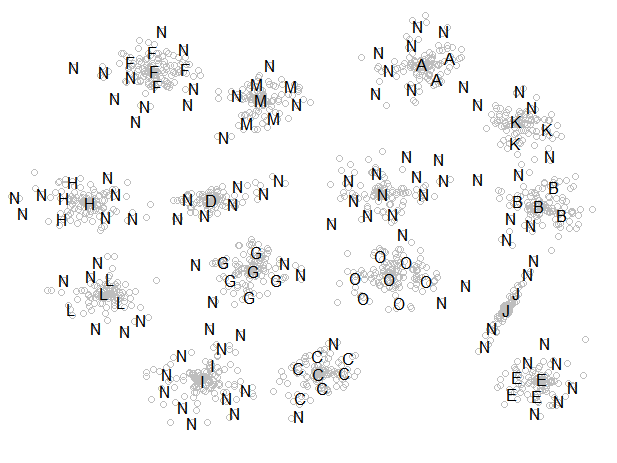
\includegraphics[width = 10cm]{weighted_issues_N_crop}
  \caption{Snapshot from Weighted Spectral Clustream on S1}
\label{fig:weighted_issues}
\end{figure}

\begin{figure}[h!]
  \centering
  \begin{subfigure}{0.45\textwidth}
    \centering
    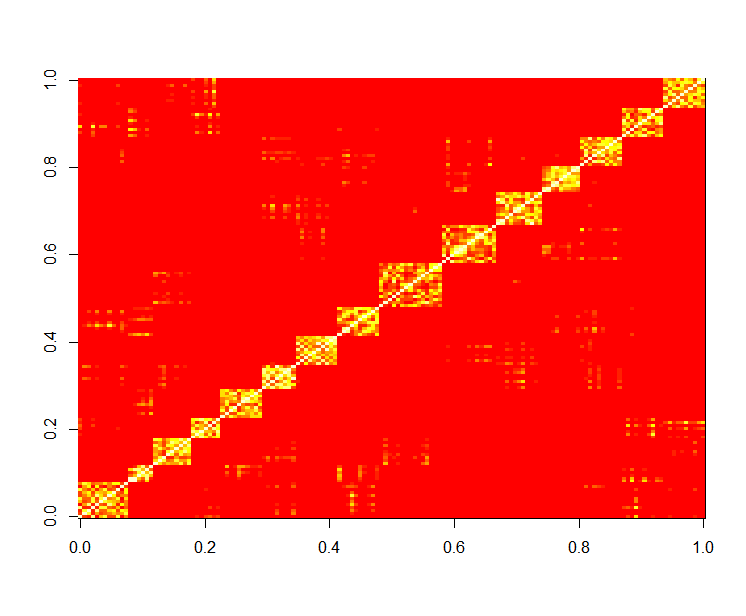
\includegraphics[width = \textwidth, height = \textwidth]{s_set/s_set_1_unweighted_affinity.png}
    \caption{Unweighted affinity matrix}
  \label{fig:unweighted_affinity}
  \end{subfigure}
  \begin{subfigure}{0.45\textwidth}
    \centering
    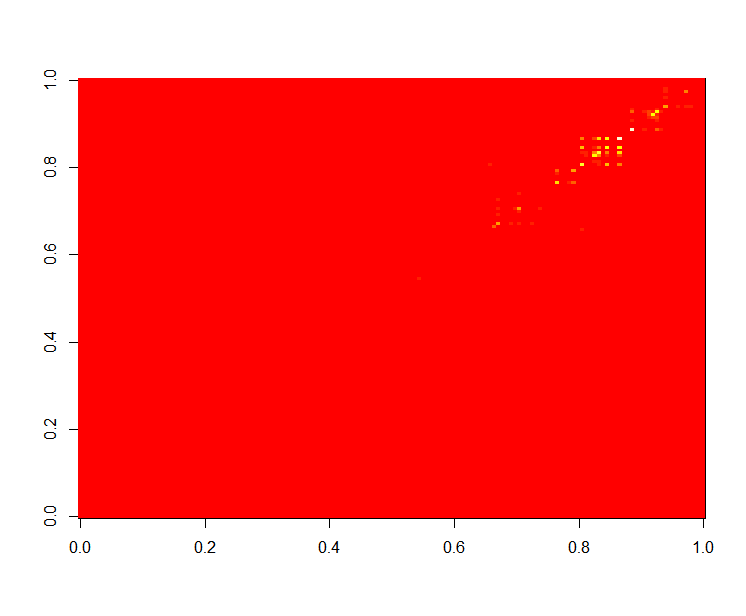
\includegraphics[width = \textwidth, height = \textwidth]{s_set/s_set_1_weighted_affinity.png}
  \caption{Weighted affinity matrix}
  \label{fig:weighted_affinity}
  \end{subfigure}
    \caption{Affinity matrices for S set 1}
  \label{fig:set_1_affinities}
\end{figure}

We can observe the affinity matrix by plotting it as an image, where bright values imply an affinity value close to one and red means the value is close to zero. Figure \ref{fig:set_1_affinities} shows an image of both the unweighted and weighted affinity for the example shown in Figure \ref{fig:weighted_issues}. The affinity matrix has dimension $150 \times 150$, with each row representing the similarities between one micro-cluster centre and the other 149. The rows and columns have been grouped so that micro-cluster centres from the same true underlying clusters are next to each other. 

We can see that in Figure \ref{fig:unweighted_affinity} the block nature of the unweighted affinity is clear. There are strong affinities between close micro-clusters, and weak affinities between distant micro-clusters making this an informative affinity matrix to use with Spectral Clustering. However in the weighted affinity matrix (Figure \ref{fig:weighted_affinity}) the block nature is not visible. Most of the values are close to zero, with only a few strong affinities. The weighting seems to have dampened the affinity matrix, incorrectly reducing the affinity of  close micro-clusters. It is possible that the use of the localised scaling parameter (See Section \ref{sec:affinity}) in the Spectral Clustering step may be interfering with the weighting of micro-clusters.  We did attempt to use a global scaling parameter instead of the localised one, however this then brought up the issue of tuning the $\sigma$ parameter, which is known to be very sensitive and is a difficulty for Spectral Clustering algorithms in general \citep{Luxburg2008}. Although performance did seem to improve with the global scaling parameter when chosen carefully, the performance was still very poor compared to Windowed Spectral Clustering and Spectral Clustream.


\subsection{Texture data}

We now investigate the performance of the clustering algorithms features extracted from textured images. The Kylberg  texture data set \citep{kylberg2011c} consists of 28 texture classes with 160 unique texture patches per class. The patches consist of $576 \times 576$ pixel images. Features for clustering were extracted using the LS2W \citep{Eckley2011} which creates 27 wavelet features from the textured images. 

A subset of 6 classes were selected,  examples of which are shown in Figure \ref{fig:texture_examples} .  The classes selected are images of two types of blanket, some canvas, a ceiling, some lentils and a screen.

\begin{figure}[h!]
\begin{subfigure}{.15\textwidth}
  \centering
  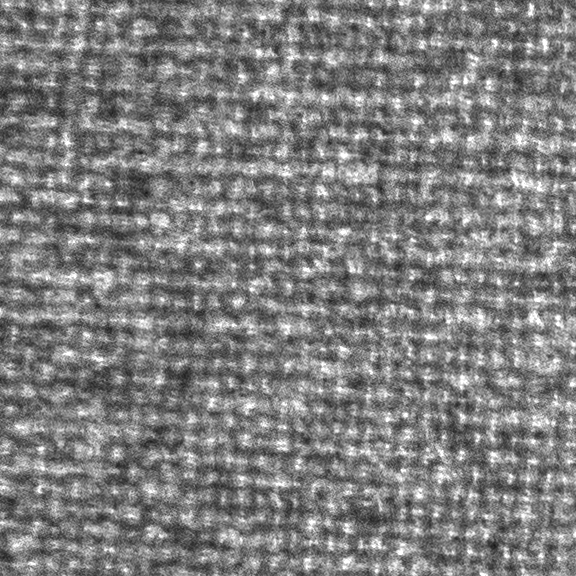
\includegraphics[width=.8\linewidth]{kylberg_examples/blanket1_001.png}
  %\caption{PCA of digits 2 and 9}
 % \label{fig:sfig1}
\end{subfigure}%
\begin{subfigure}{.15\textwidth}
  \centering
  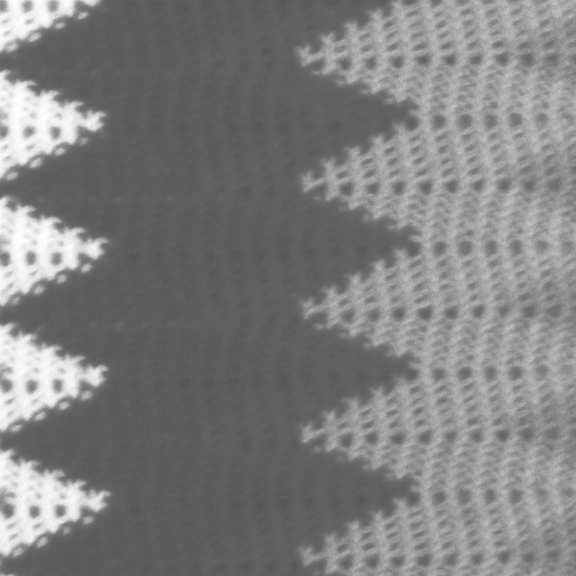
\includegraphics[width=.8\linewidth]{kylberg_examples/blanket2_001.png}
  %\caption{Purity digits 2 and 9}
%  \label{fig:sfig2}
\end{subfigure}
\begin{subfigure}{.15\textwidth}
  \centering
  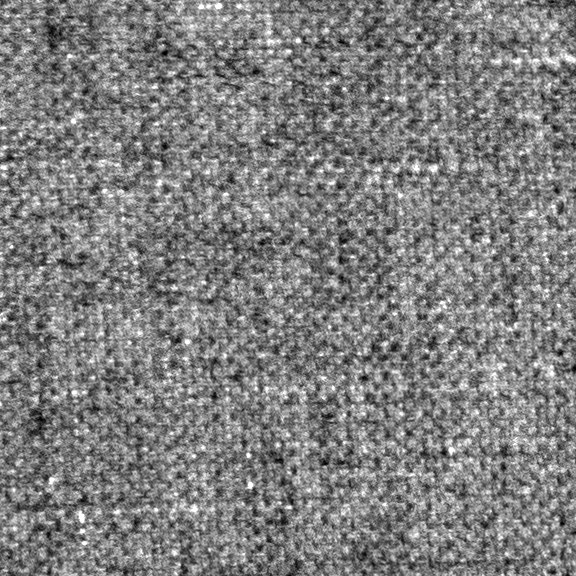
\includegraphics[width=.8\linewidth]{kylberg_examples/canvas1_001.png}
  %\caption{V-measure digits 2 and 9}
%  \label{fig:sfig2}
\end{subfigure}
\begin{subfigure}{.15\textwidth}
  \centering
  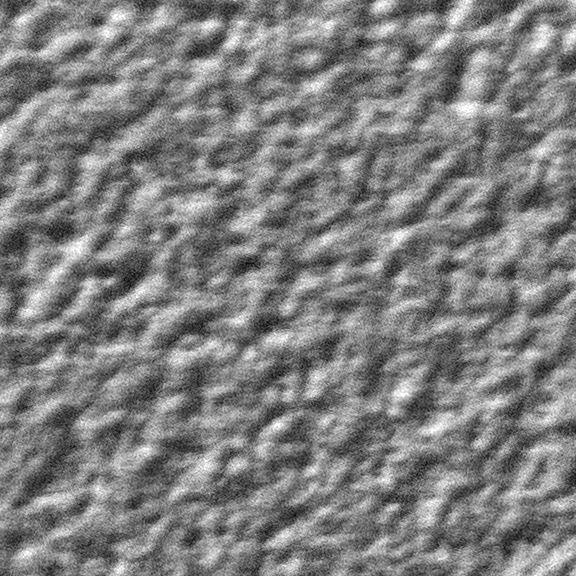
\includegraphics[width=.8\linewidth]{kylberg_examples/ceiling1_001.png}
  %\caption{PCA of digits 2 and 9}
 % \label{fig:sfig1}
\end{subfigure}%
\begin{subfigure}{.15\textwidth}
  \centering
  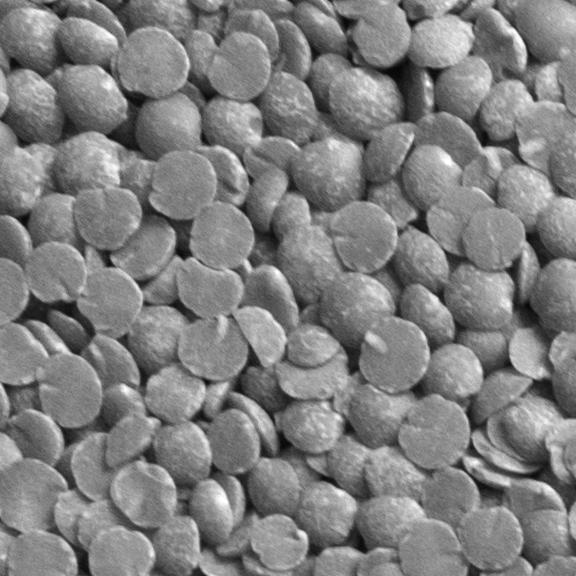
\includegraphics[width=.8\linewidth]{kylberg_examples/lentils1_001.png}
  %\caption{Purity digits 2 and 9}
%  \label{fig:sfig2}
\end{subfigure}
\begin{subfigure}{.15\textwidth}
  \centering
  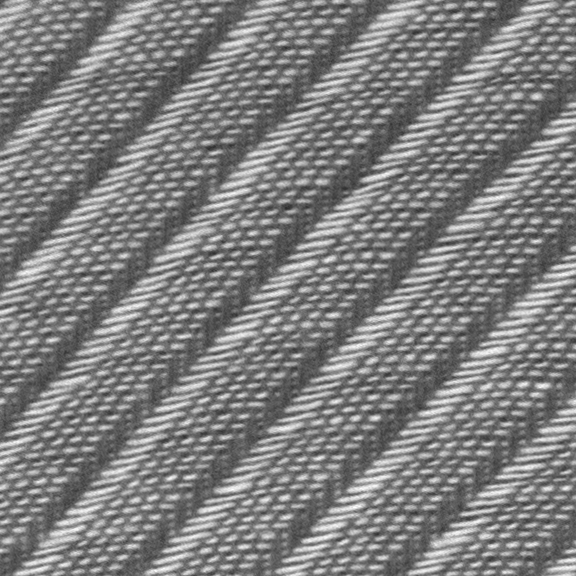
\includegraphics[width=.8\linewidth]{kylberg_examples/screen1_001.png}
  %\caption{V-measure digits 2 and 9}
%  \label{fig:sfig2}
\end{subfigure}

\begin{subfigure}{.15\textwidth}
  \centering
  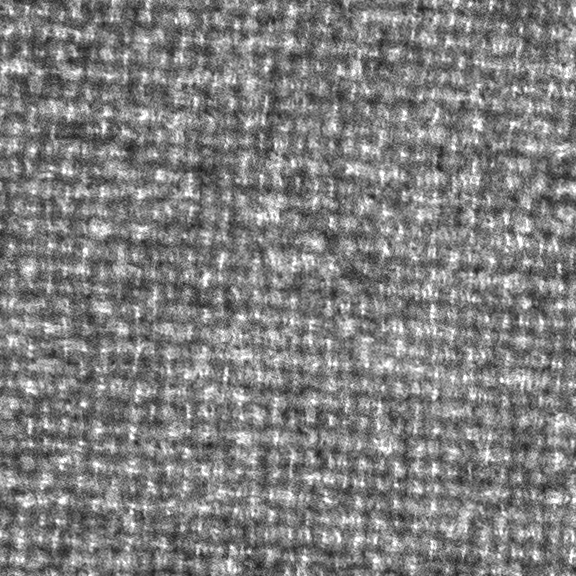
\includegraphics[width=.8\linewidth]{kylberg_examples/blanket1_002.png}
  %\caption{PCA of digits 2 and 9}
 % \label{fig:sfig1}
\end{subfigure}%
\begin{subfigure}{.15\textwidth}
  \centering
  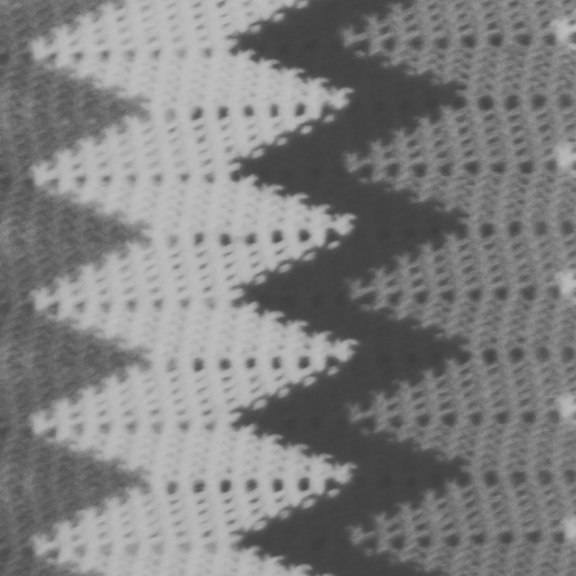
\includegraphics[width=.8\linewidth]{kylberg_examples/blanket2_002.png}
  %\caption{Purity digits 2 and 9}
%  \label{fig:sfig2}
\end{subfigure}
\begin{subfigure}{.15\textwidth}
  \centering
  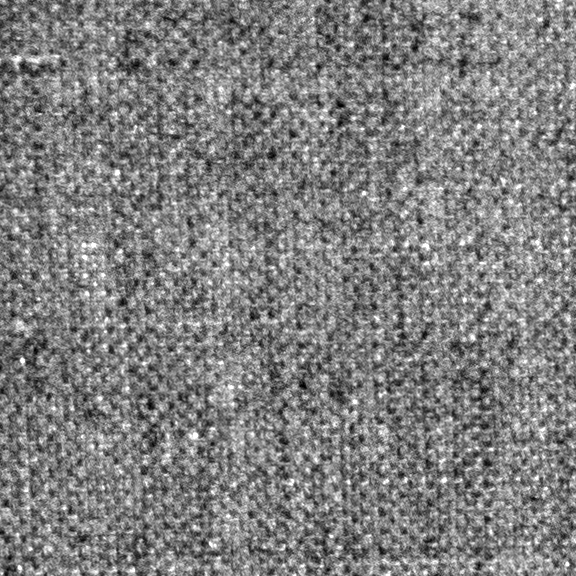
\includegraphics[width=.8\linewidth]{kylberg_examples/canvas1_002.png}
  %\caption{V-measure digits 2 and 9}
%  \label{fig:sfig2}
\end{subfigure}
\begin{subfigure}{.15\textwidth}
  \centering
  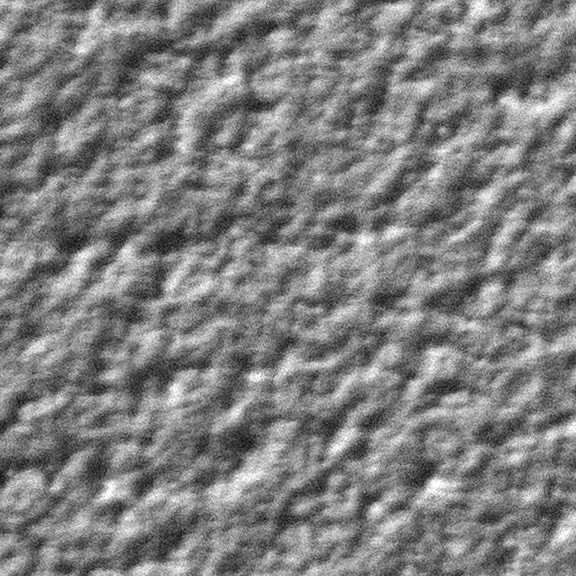
\includegraphics[width=.8\linewidth]{kylberg_examples/ceiling1_002.png}
  %\caption{PCA of digits 2 and 9}
 % \label{fig:sfig1}
\end{subfigure}%
\begin{subfigure}{.15\textwidth}
  \centering
  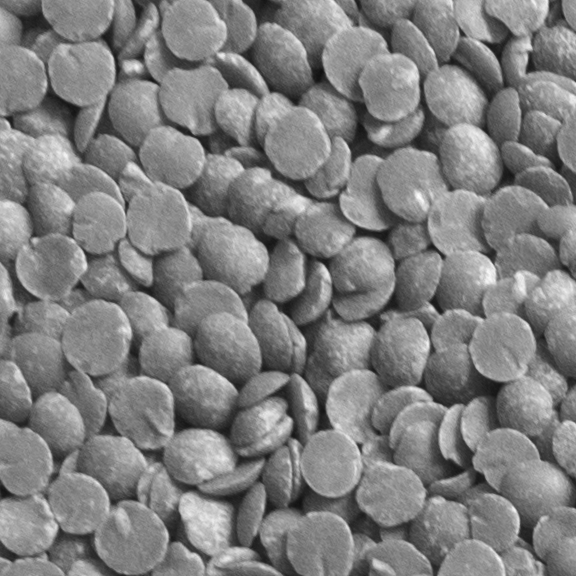
\includegraphics[width=.8\linewidth]{kylberg_examples/lentils1_002.png}
  %\caption{Purity digits 2 and 9}
%  \label{fig:sfig2}
\end{subfigure}
\begin{subfigure}{.15\textwidth}
  \centering
  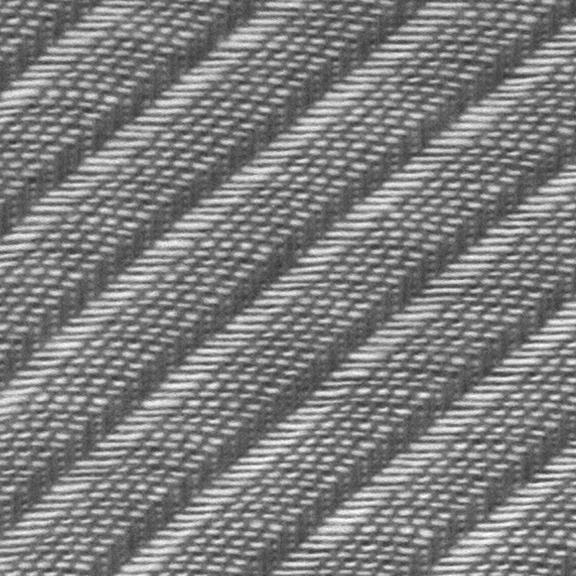
\includegraphics[width=.8\linewidth]{kylberg_examples/screen1_002.png}
  %\caption{V-measure digits 2 and 9}
%  \label{fig:sfig2}
\end{subfigure}

\begin{subfigure}{.15\textwidth}
  \centering
  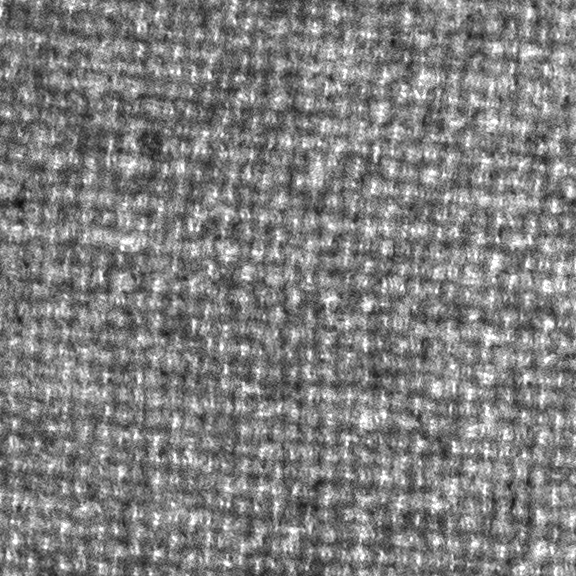
\includegraphics[width=.8\linewidth]{kylberg_examples/blanket1_003.png}
  %\caption{PCA of digits 2 and 9}
 % \label{fig:sfig1}
\end{subfigure}%
\begin{subfigure}{.15\textwidth}
  \centering
  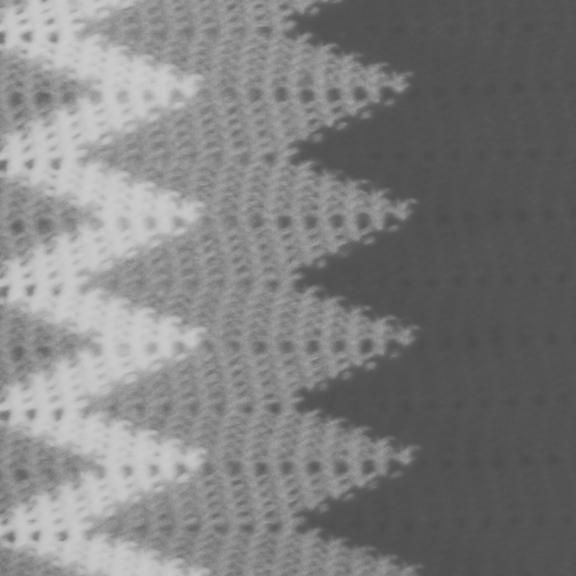
\includegraphics[width=.8\linewidth]{kylberg_examples/blanket2_003.png}
  %\caption{Purity digits 2 and 9}
%  \label{fig:sfig2}
\end{subfigure}
\begin{subfigure}{.15\textwidth}
  \centering
  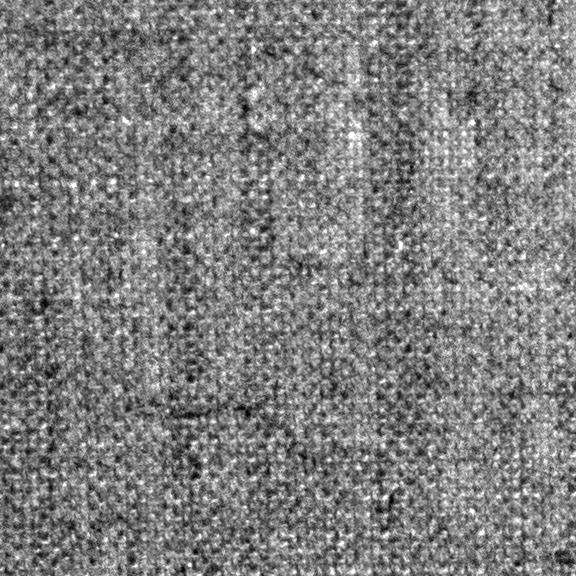
\includegraphics[width=.8\linewidth]{kylberg_examples/canvas1_003.png}
  %\caption{V-measure digits 2 and 9}
%  \label{fig:sfig2}
\end{subfigure}
\begin{subfigure}{.15\textwidth}
  \centering
  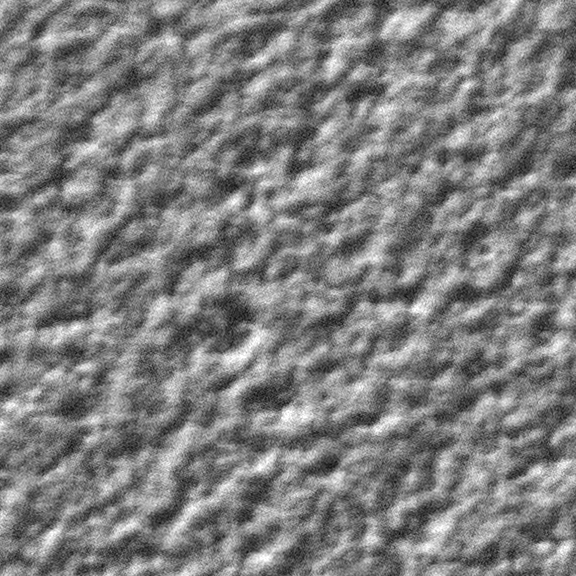
\includegraphics[width=.8\linewidth]{kylberg_examples/ceiling1_003.png}
  %\caption{PCA of digits 2 and 9}
 % \label{fig:sfig1}
\end{subfigure}%
\begin{subfigure}{.15\textwidth}
  \centering
  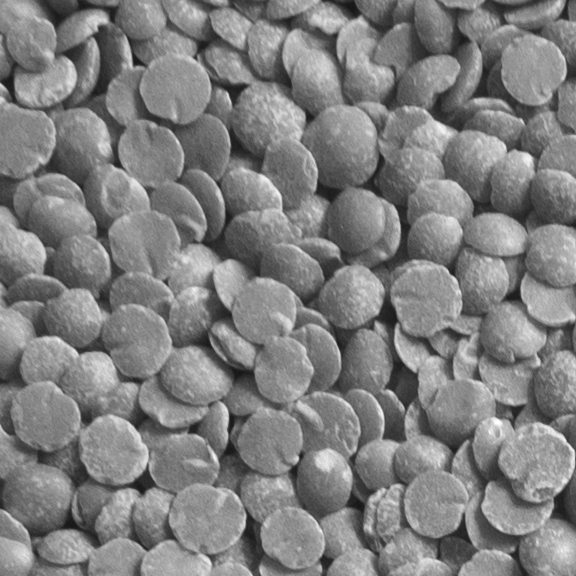
\includegraphics[width=.8\linewidth]{kylberg_examples/lentils1_003.png}
  %\caption{Purity digits 2 and 9}
%  \label{fig:sfig2}
\end{subfigure}
\begin{subfigure}{.15\textwidth}
  \centering
  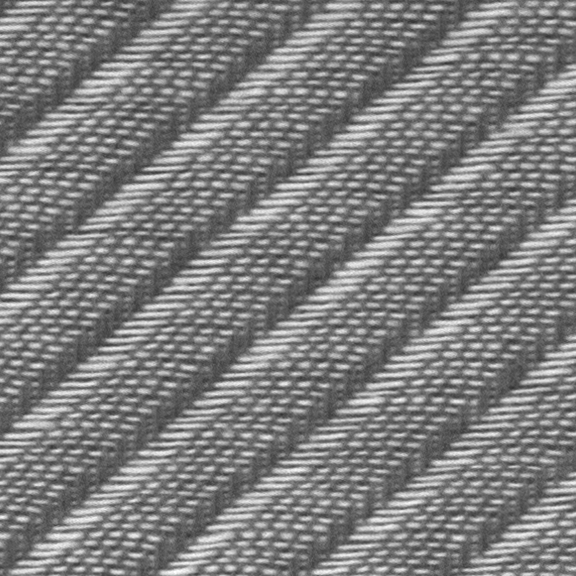
\includegraphics[width=.8\linewidth]{kylberg_examples/screen1_003.png}
  %\caption{V-measure digits 2 and 9}
%  \label{fig:sfig2}
\end{subfigure}
\caption{Three examples from each of the 6 different texture tiles used in the streaming data set. The texture classes are (L-R) Blanket 1, Blanket 2, Canvas, Ceiling, Lentils and Screen}
\label{fig:texture_examples}
\end{figure}

The performance plots for the texture data are shown in Figure \ref{fig:texture_results}. Here we  do see a difference between Windowed Spectral Clustering and Unweighted Spectral Clustream, the windowed approach is generally performing better. Once again Weighted Spectral Clustream does not perform well, and performance declines as the stream progresses.

\begin{figure}[h!]
\begin{subfigure}{.5\textwidth}
  \centering
  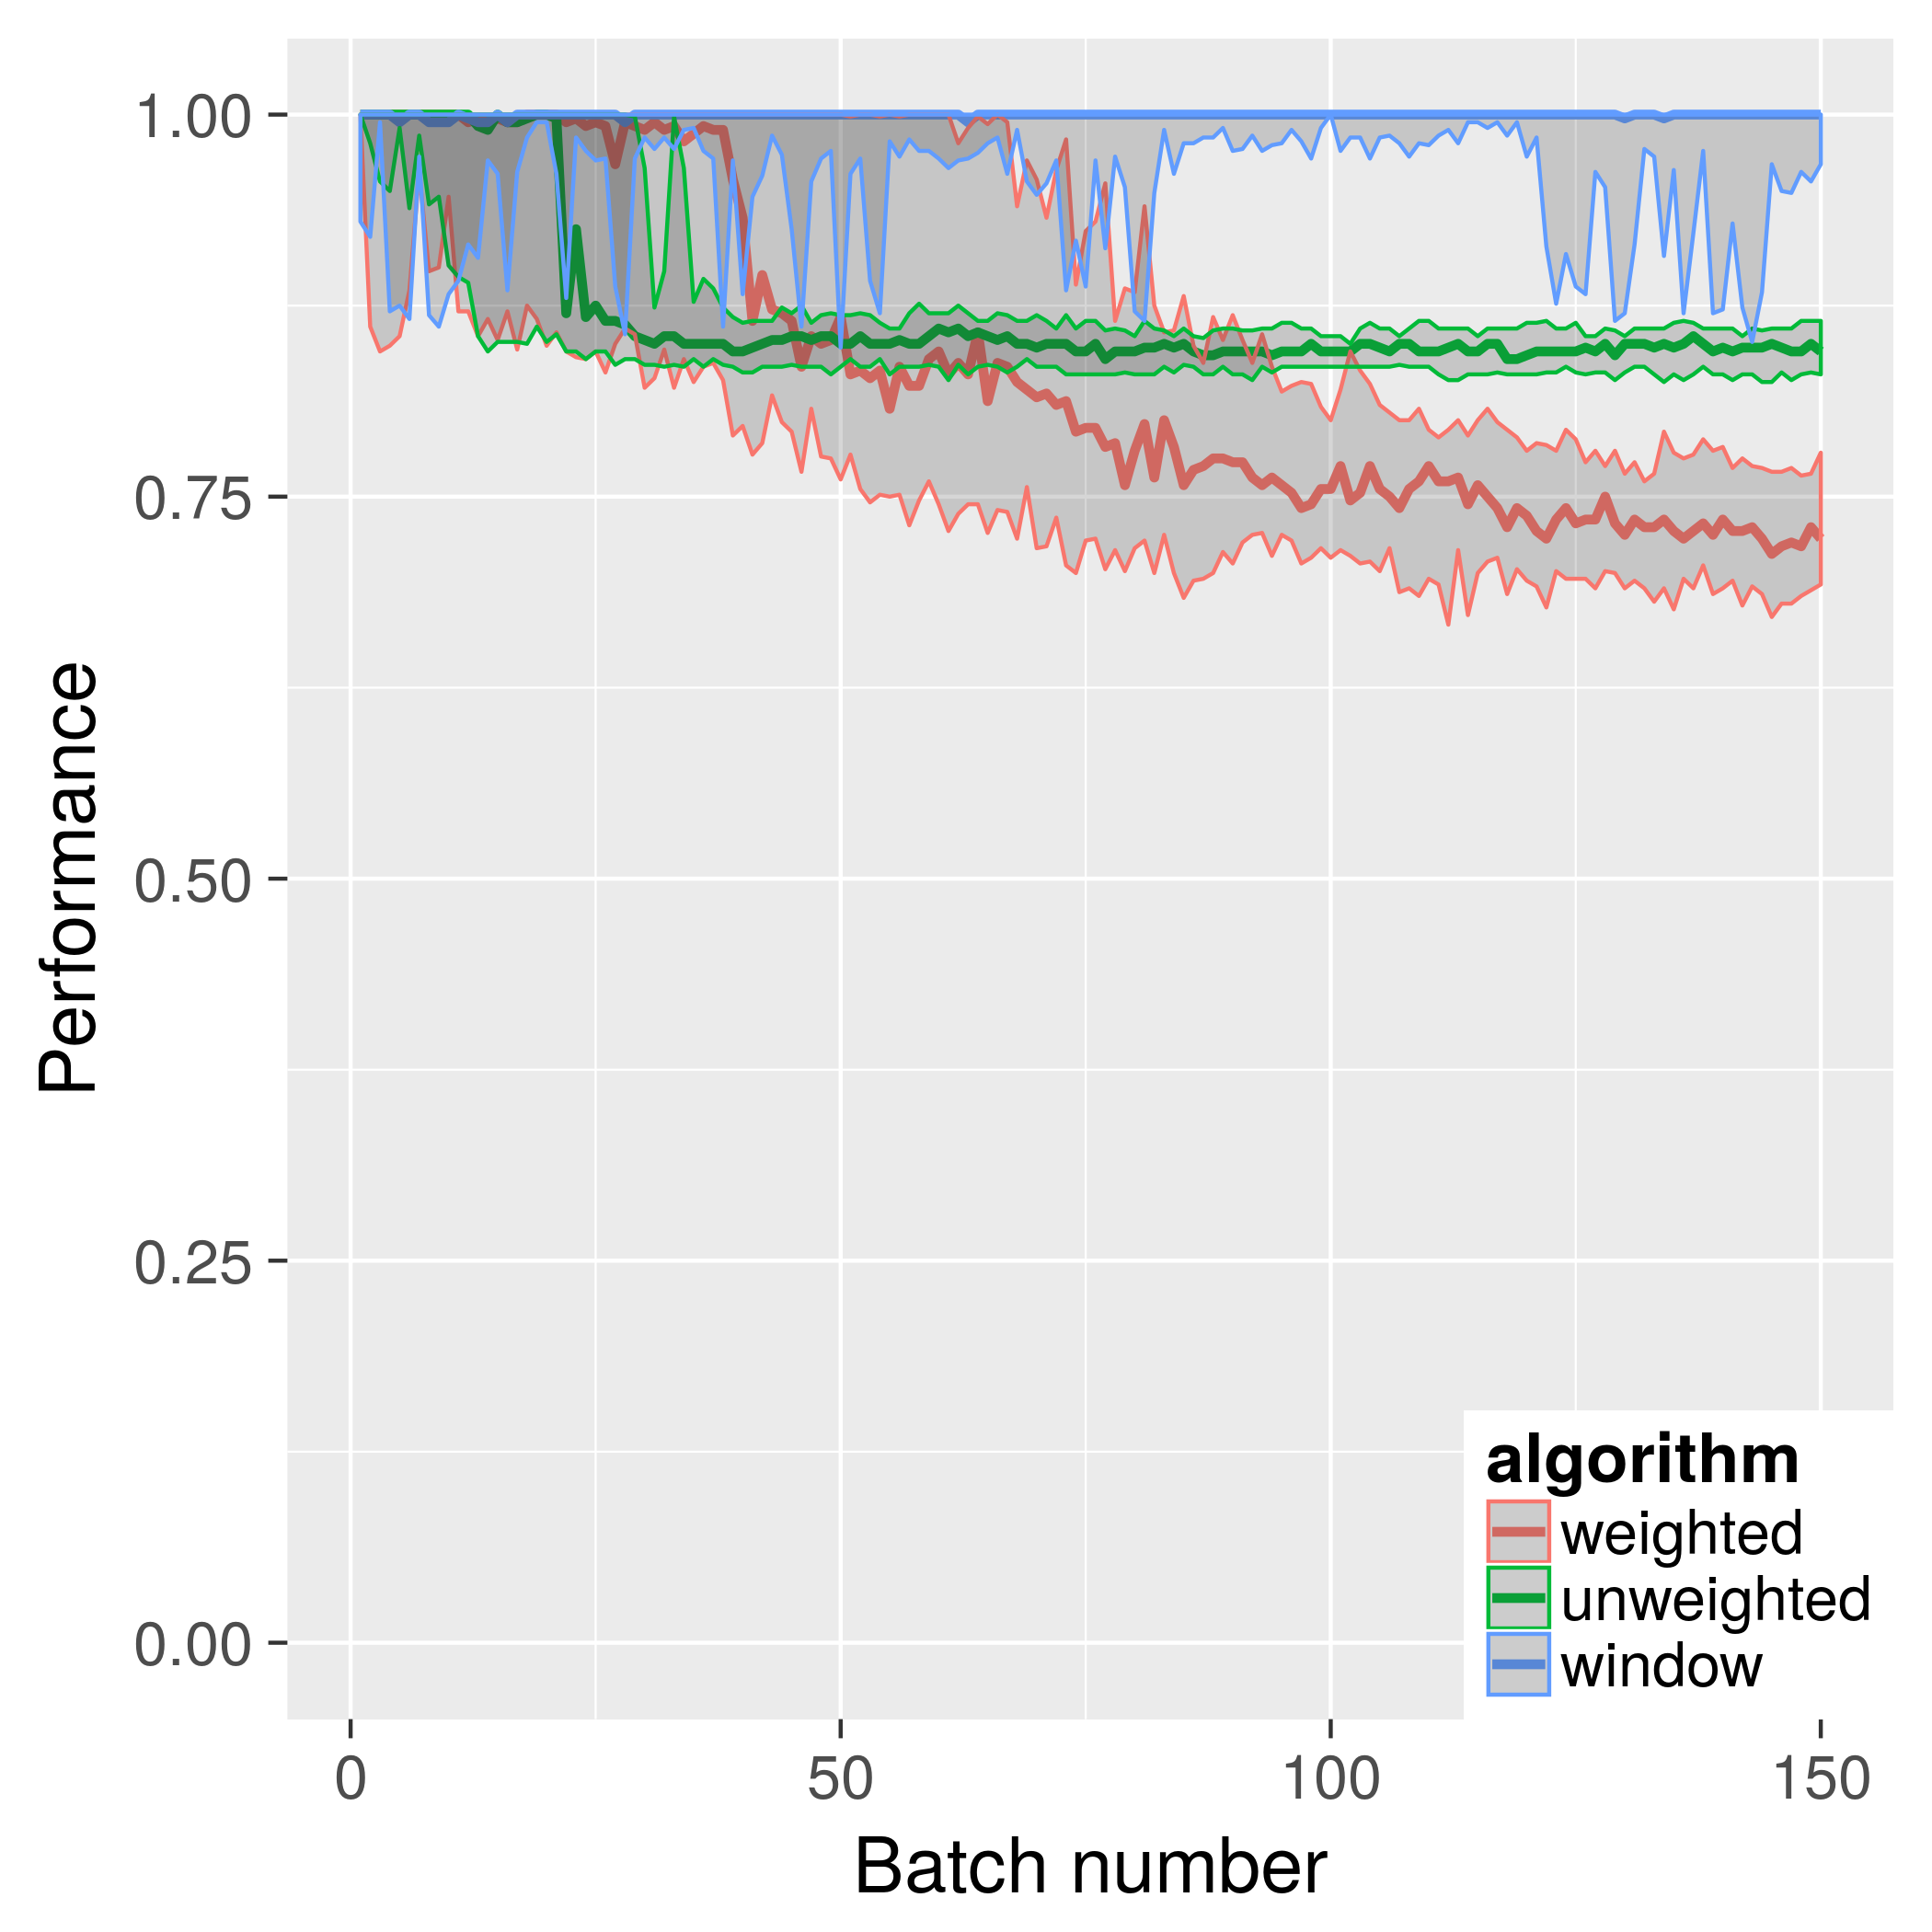
\includegraphics[width=1\linewidth]{texture/texture_with_weighted_ci_one_size_purity}
  \caption{Texture Purity}
 % \label{fig:sfig1}
\end{subfigure}%
\begin{subfigure}{.5\textwidth}
  \centering
  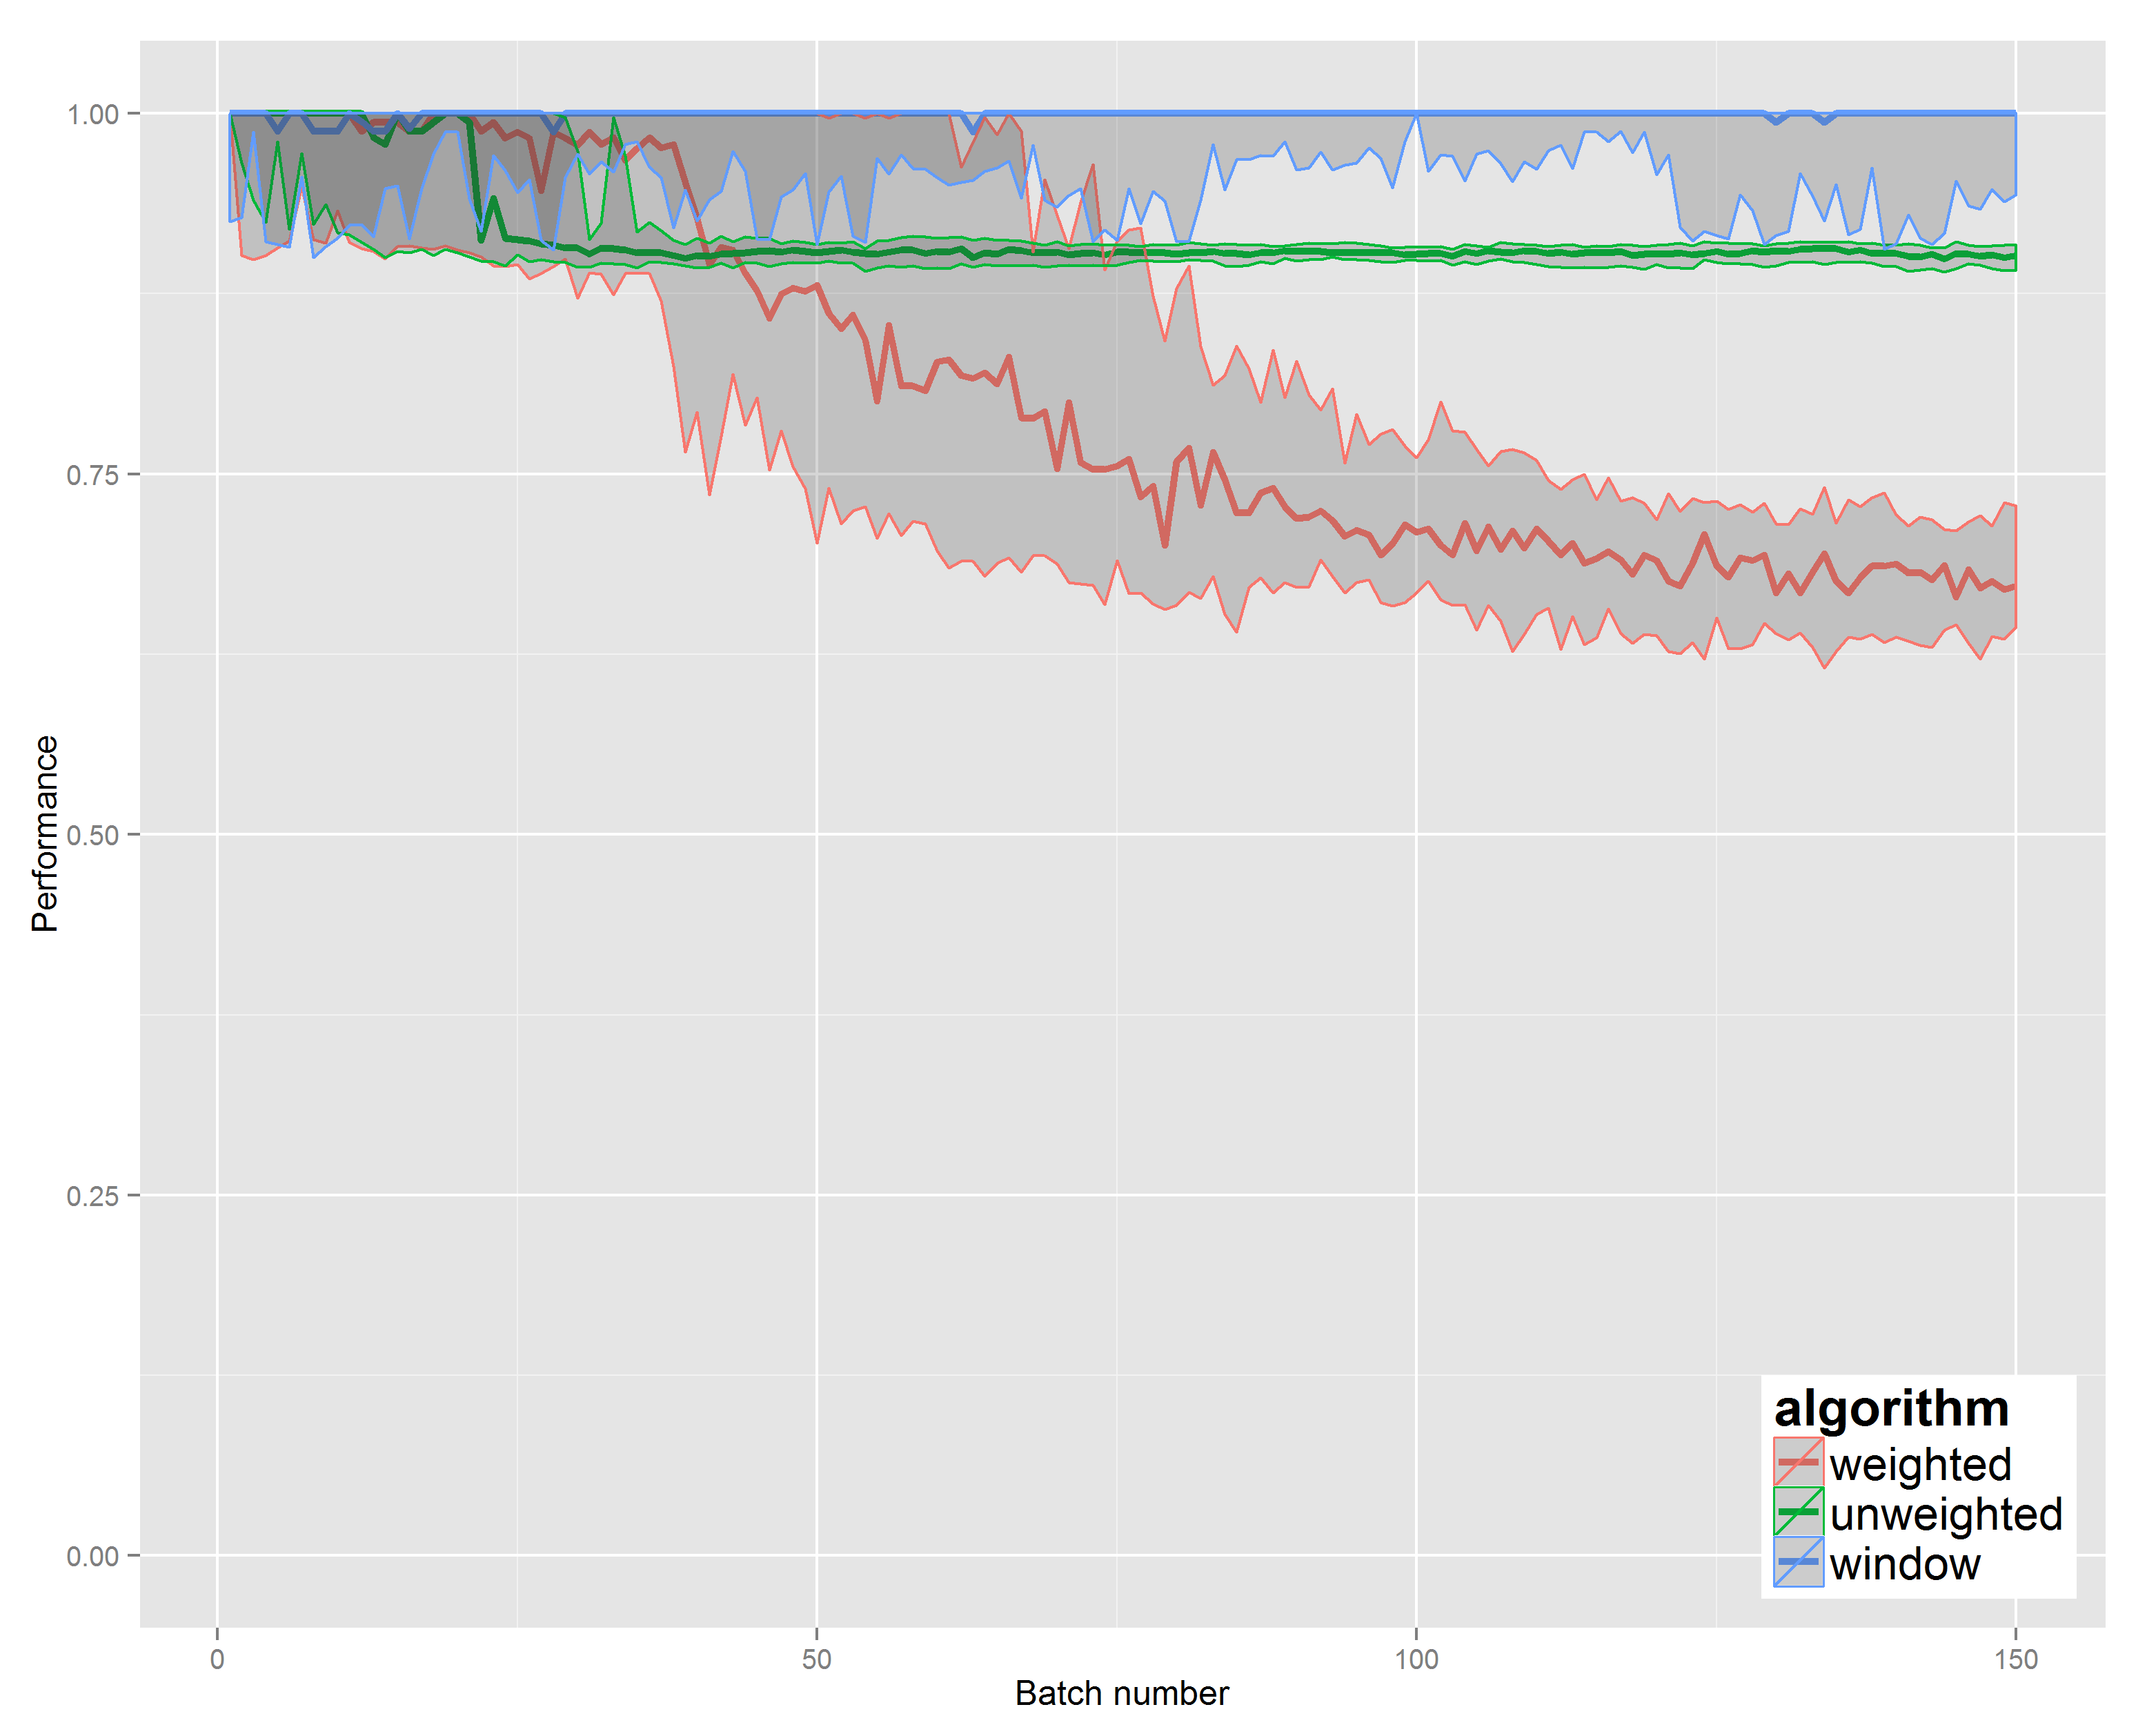
\includegraphics[width=1\linewidth]{texture/texture__with_weighted_ci_one_size_vmeasure}
  \caption{Texture V-measure}
%  \label{fig:sfig2}
\end{subfigure}
\caption{Texture Results}
\label{fig:texture_results}
\end{figure}


The poor performance of Weighted Spectral Clustream was observed on all other data sets investigated and therefore the results from this algorithm  will be dropped from any further performance plots in order to focus more on the behaviour of the other two algorithms.  From now on, we will refer to Unweighted Spectral Clustream simply as Spectral Clustream.

\subsection{Pendigit data}
This section and the next will use the UCI Pendigit data set which was introduced in \cite{Alimoglu1996} and is available is for download \citep{Lichman2013}. The data set consists of 250 samples of hand drawn digits of the numbers 0-9 taken from 44 writers. The data was collected using a pressure sensitive tablet. There are 16 features each relating to the co-ordinate information taken from the input tablet. We restrict our analysis to pairwise comparison of digits. For example we attempt to cluster the digits 0 and 1, and treat the data as if it is arriving in a constant data stream.

The results for a selection of the pairwise digits are shown in Figure \ref{fig:uci_pendigits}. The first column displays the digit data in PCA space, the second column shows the purity, and the third column shows the V-measure. Both algorithms show similar performance in the plots shown (and in all the other pairwise combinations which were run).  It can be noted that V-measure is lower than purity, which might imply that the resulting clusters are homogeneous but not complete (see Section \ref{sec:performance}). 

\begin{figure}[H]

\begin{subfigure}{.3\textwidth}
  \centering
  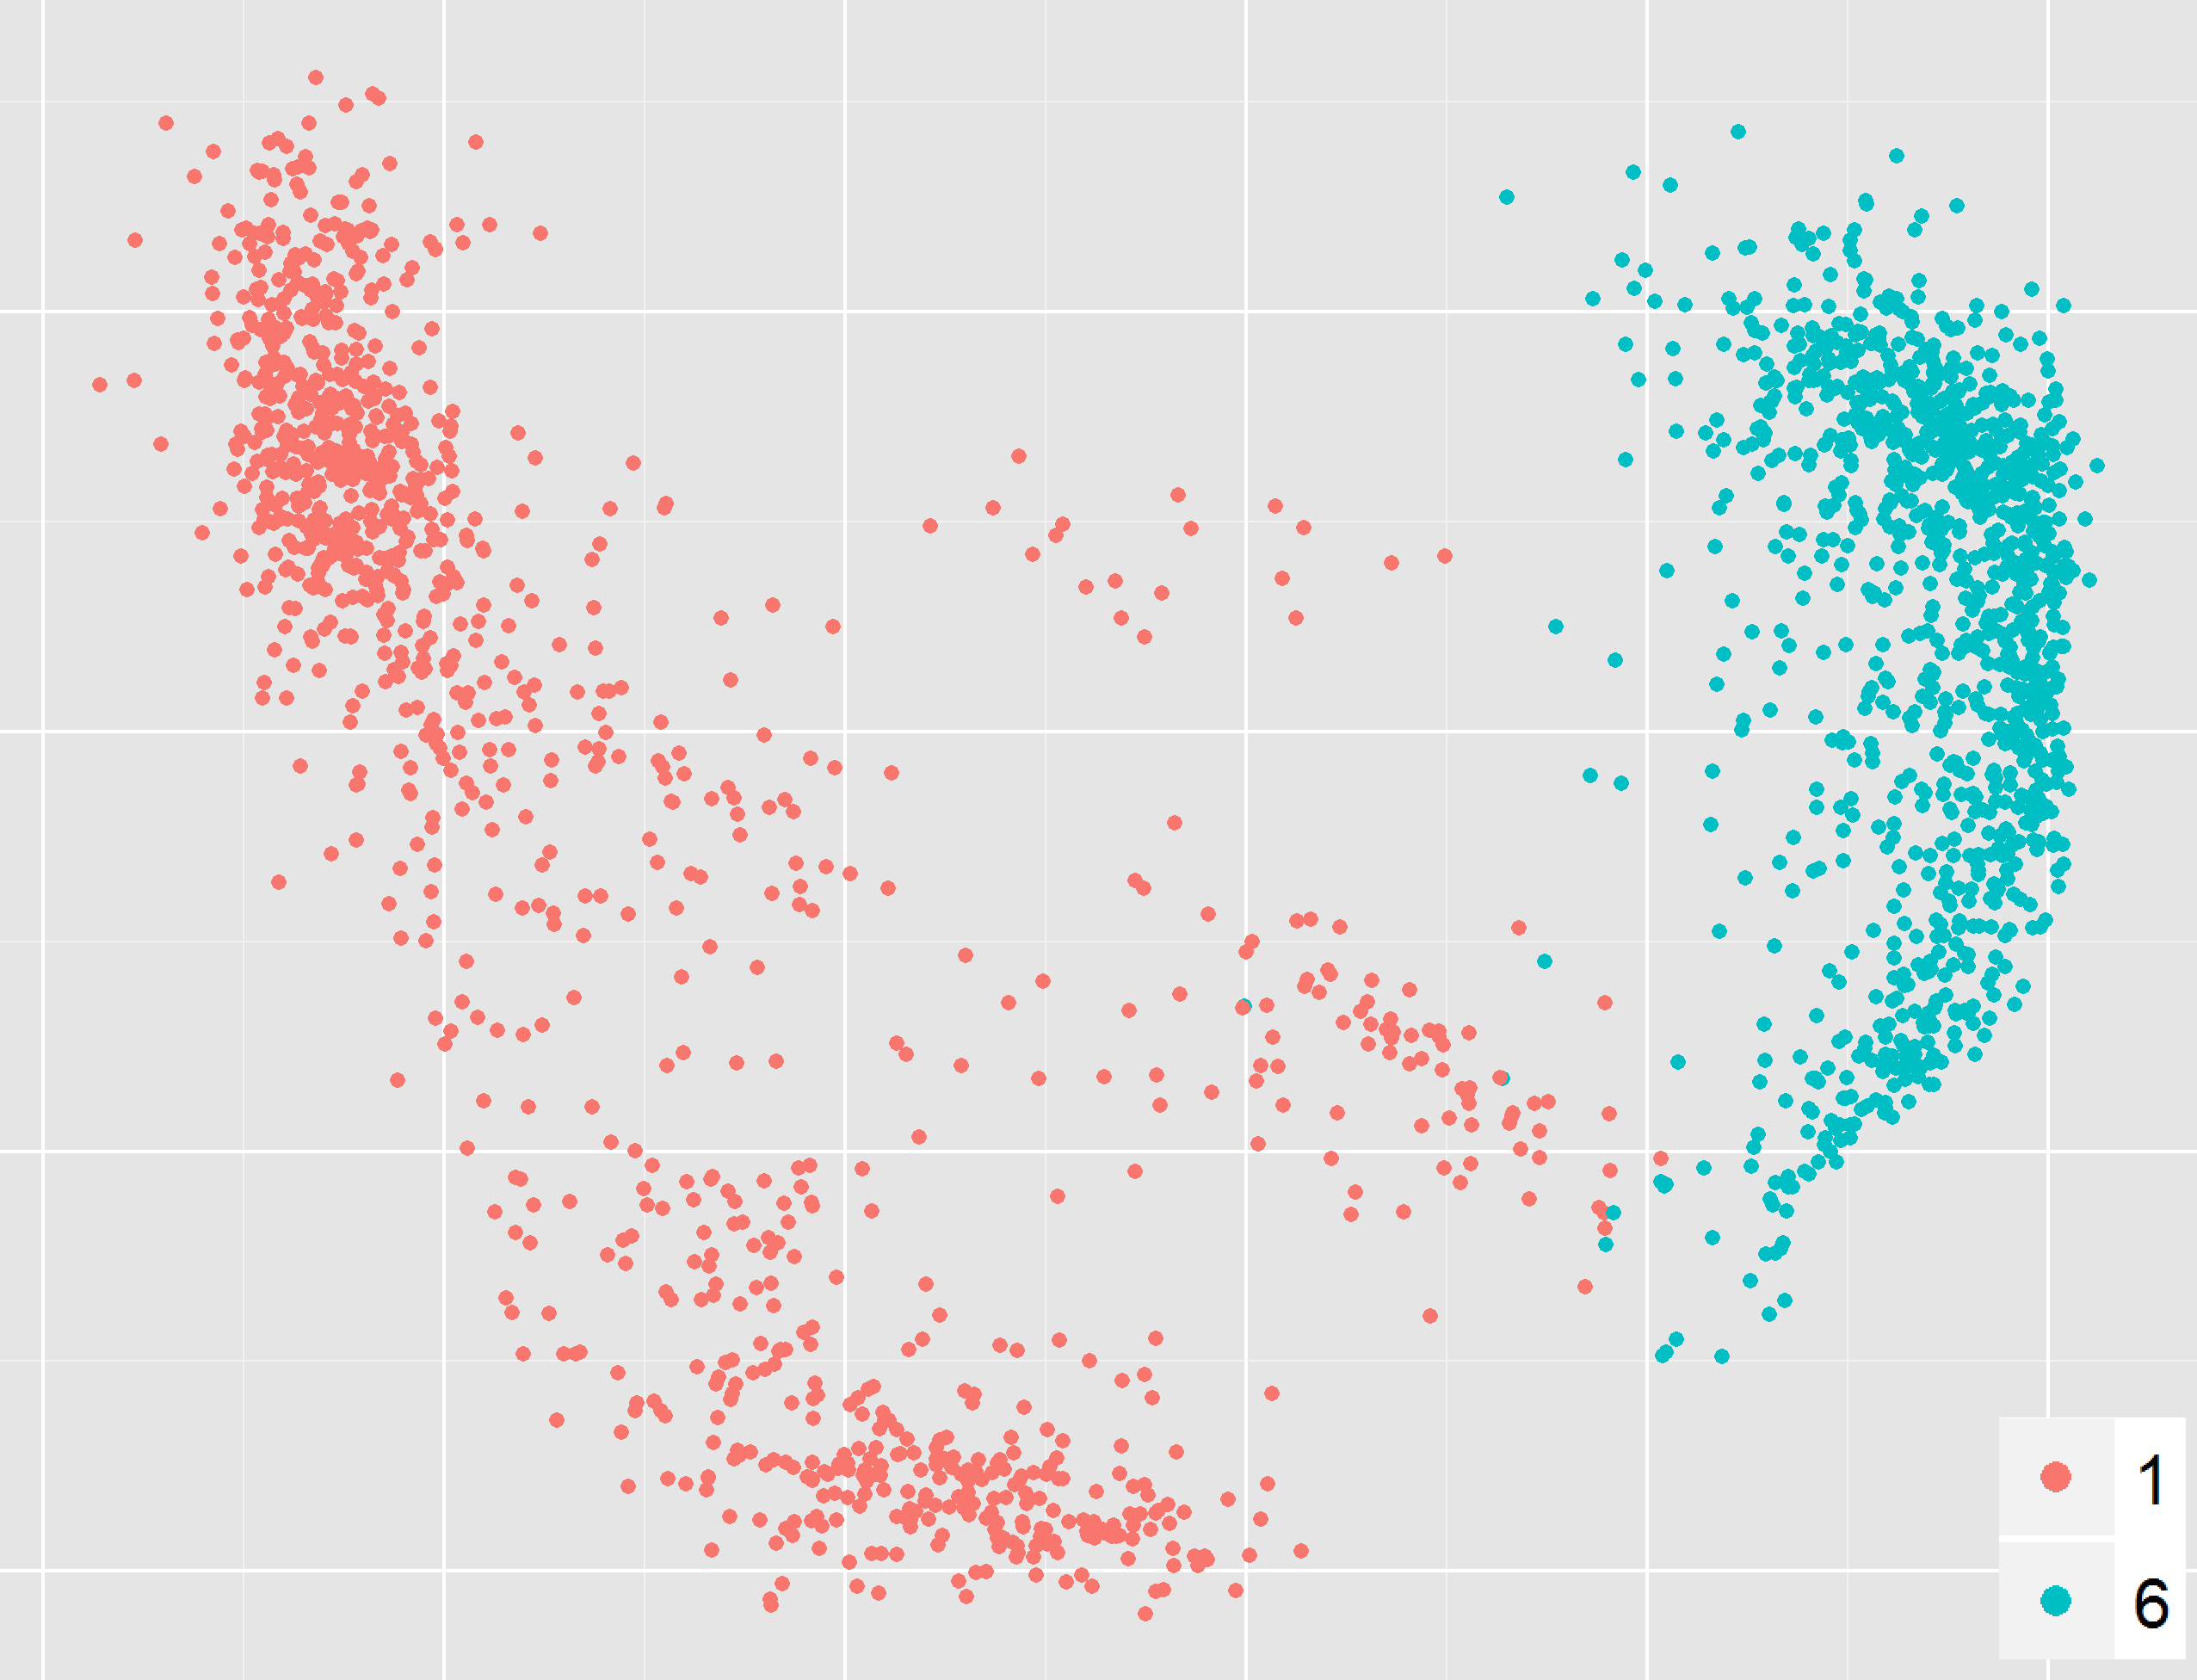
\includegraphics[width=\linewidth]{PCA_pendigits_pairwise/pairwise_1_6_cropped.png}
  \caption{PCA of digits 1 and 6}
 % \label{fig:sfig1}
\end{subfigure}%
\begin{subfigure}{.3\textwidth}
  \centering
  \includegraphics[width=\linewidth]{pendigits_2_alg/uci_pendigits_16_ci_one_size_purity.png}
  \caption{Purity digits 1 and 6}
%  \label{fig:sfig2}
\end{subfigure}
\begin{subfigure}{.3\textwidth}
  \centering
  \includegraphics[width=\linewidth]{pendigits_2_alg/uci_pendigits_16_ci_one_size_vmeasure.png}
  \caption{V-measure digits 1 and 6}
%  \label{fig:sfig2}
\end{subfigure}

\begin{subfigure}{.3\textwidth}
  \centering
  \includegraphics[width=\linewidth]{PCA_pendigits_pairwise/pairwise_4_7_cropped.png}
  \caption{PCA of digits 4 and 7}
 % \label{fig:sfig1}
\end{subfigure}%
\begin{subfigure}{.3\textwidth}
  \centering
  \includegraphics[width=\linewidth]{pendigits_2_alg/uci_pendigits_47_ci_one_size_purity.png}
  \caption{Purity digits 4 and 7}
%  \label{fig:sfig2}
\end{subfigure}
\begin{subfigure}{.3\textwidth}
  \centering
  \includegraphics[width=\linewidth]{pendigits_2_alg/uci_pendigits_47_ci_one_size_vmeasure.png}
  \caption{V-measure digits 4 and 7}
%  \label{fig:sfig2}
\end{subfigure}
\caption{Pendigits Pairwise - Spectral Clustream and Windowed Spectral Clustering}
\label{fig:uci_pendigits}
\end{figure}

\subsection{Non-stationary data}
\label{sec:non_stationary}

So far we have considered only stationary data streams. The main challenge for clustering algorithms for data streams is adapting to changes in the data stream. In order to create data streams with a non stationary distribution we introduce a change into the data stream. To construct a data stream we choose three digits in the Pendigits data set (for example 4, 8 and 9). The start of the data stream consists only of 2 digits (4 and 8). Half way through the stream, we replace  the second digit with the third digits (so now we observe values 4 and 9 rather than 4 and 8). By swapping the digits in this manner we can avoid the difficult issue of having to select a number of clusters, as we always observe only two clusters.  The example set is ``Pendigits 48 49'' - first we observe features from digits 4 and 8, and we switch to observing features from digits 4 and 9 half way through the stream. Figure \ref{fig:48_49_pca} shows the PCA space for all  three digits. There is quite a bit of overlap between digits 4 and 9, which makes the data stream quite tricky to cluster. 

\begin{figure}[!h]
  \centering
 \includegraphics[width=.6\linewidth]{evolving_pen/evolving_pen_48_49_truth.png}  
\caption{PCA plot for the Pendigits 4, 8 and 9}
\label{fig:48_49_pca}
\end{figure}

We ran Spectral Clustream and Windowed Spectral Clustering on this  data stream. We have included a number of different values for the number of micro-clusters  $q \in (50, 100, 150, 200)$ and also ran Windowed Spectral with window sizes $w \in( 50,100,150, 200)$. The results in terms of purity and v-measure are shown in Figure \ref{fig:results_48-49}.  In the plots the dashed lines show the Windowed Spectral Clustering and the full lines are Unweighted Spectral Clustream. The colours indicate different values for the number of micro-clusters/window size. 

%Due to the nature of algorithms with windowing, we would expect Windowed Spectral Clustering to adapt quickly to this change given the window size is fairly small ($w = 150$). The initial results showed Spectral Clustream performing poorly after the change, and struggling to recover. These results will be shown at the end of the section, and fix is suggested to correct the poor behaviour. First, in order to understand why Spectral Clustream was performing badly lets consider a specific example. 

%%%%%%%
\begin{figure}[!h]
        \centering
        \begin{subfigure}[b]{0.47\textwidth}
          \includegraphics[width=\textwidth]{standard_alt/ci_evolving_pen_48_49_standard_purity.png}         
                 \caption{Purity}
                 \label{fig:ps_4849}
        \end{subfigure}
        \begin{subfigure}[b]{0.47\textwidth}
          \includegraphics[width=\textwidth]{standard_alt/ci_evolving_pen_48_49_standard_vmeasure.png}
                 \caption{Vmeasure}
                 \label{fig:vs_4849}
        \end{subfigure}
\caption{Purity and V-measure for  Pendigits 48-49}
\label{fig:results_48-49}
\end{figure}

The initial results show that Spectral Clustream does not perform well after the change is observed. Both purity and v-measure drop dramatically low and do not recover. A fix is required in order for Spectral Clustream to deal with the change in the data stream. In order to understand why performance drops at the change and discover how to fix this we need to look closely at the behaviour of the  micro-clusters. Figure \ref{fig:stream_1} shows the micro-clusters for Spectral Clustream at the start of the stream (directly after initialisation). The grey points show all data seen up until this time and the blue points indicate the next 200 points to be observed (the test set used for our performance measures.) The crosses indicate locations of micro-cluster centres, and their colour indicates which overall cluster they have been assigned to using the Spectral Clustering algorithm. 

\begin{figure}
\begin{subfigure}{.5\textwidth}
  \centering
  \includegraphics[width=\textwidth]{evolving_pen/evolving_pen_48_49_1_crop.png}  
  \caption{Stream at time t = 1}
  \label{fig:stream_1}
\end{subfigure}
\begin{subfigure}{.5\textwidth}
  \centering
  \includegraphics[width=\textwidth]{evolving_pen/evolving_pen_48_49_100_crop.png}  
  \caption{Stream at time t = 1000 }
  \label{fig:stream_1000}
\end{subfigure}
\caption{Micro-cluster centres for the Pendigits 48, 49}
\label{stream_1_100}
\end{figure}

In Figure \ref{fig:stream_1}, at time step 1, the micro-cluster centres are well distributed over the grey data points and also the blue test points. The Spectral Clustering mostly segments the micro-cluster centres correctly into the left and right clusters. 

At time step 1000 (Figure \ref{fig:stream_1000}), we have begun observing the new cluster (digit 9 in the top left corner) and are no longer receiving data points from digit 8. This is shown as all of the test data points (light blue) are in either the bottom left corner (digit 4) and top left corner (digit 9). We see that the micro-cluster centres (crosses) are spread out over all the data including the defunct cluster of digit 8 (the grey data points on the right hand side of the plot).  The reason that there are still micro-cluster centres located in the cluster 8 region is because of the deletion policy that Clustream uses.

Clustream requires the number of micro-clusters to remain fixed for the duration of the stream. As discussed in Section \ref{sec:microSpec}, if an arriving data point does not have a suitable micro-cluster to merge into, a new micro-cluster is formed. However, since the total number of micro-clusters is fixed, this means that we need to either delete an old micro-cluster if it is suitably old, or combine two close ones. This is the only way that micro-clusters can be deleted in Clustream.  A micro-cluster $i$ is defined to be suitably old if it's relevancy $r(M_i)$ is less than the relevancy threshold $\delta$, as defined and discussed in equation \eqref{eq:clustream_deletion}.

In practice it is difficult to select the best value of $\delta$. If $\delta$ is set too high, Clustream will delete too often and therefore emerging new micro-clusters may not be allowed to develop fully. If $\delta$ is set too small then old clusters will stay in the system much longer than required. This is an example of when $\delta$ is possibly too small, as the algorithm seems unwilling to discard old micro-clusters. %One way to improve the algorithm would be to change the Clustream deletion policy to something more intuitive, perhaps by removing the assumption that the time stamps are normally distributed. However, due to Clustream's success I wish to keep the algorithm as close to the original as possible. 

Often, storing old micro-cluster centres  isn't a problem. Keeping old micro-cluster centres is a useful way to retain some historical data about the data stream. Also, in the case where a cluster disappears for some time and then re-emerges later in the stream, retaining old micro-cluster centres may speed up the learning when the old cluster re-emerges. These type of scenarios can occur regularly in any sort of cyclic data, such as any shopping data which has seasonality. 

The problem arises when the old micro-cluster centres are used in the Spectral Clustering step. By including these old centres in the Spectral Clustering, the algorithm technically has centres from three clusters (digits 4, 8 and 9), but we have asked the Spectral Clustering algorithm to find two clusters. In the example above in Figure \ref{fig:stream_1000}, we see that the two clusters on the left that we are trying to separate are grouped together as one, because of the inclusion of the old micro-cluster centres on the right of the plot.

The proposed solution to deal with these micro-cluster centres is as follows. Before the macro-clustering step is complete, identify the micro-clusters of interest. In this setting, we find the micro-clusters which the test data are closest to. Then use only these relevant micro-cluster centres to perform the Spectral Clustering. Figure \ref{fig:stream_standard_alt} compares the  previous method with the proposed alteration. Figure \ref{fig:stream_1_repeat} shows the standard algorithm at t = 1000 (this is a duplicate of Figure \ref{fig:stream_1000} repeated for comparison purposes). Figure \ref{fig:stream_100_alt} shows the clustering of the micro-cluster centres when the  Alternative Spectral Clustream is used. 

\begin{figure}
\begin{subfigure}{.5\textwidth}
  \centering
  \includegraphics[width=\textwidth]{evolving_pen/evolving_pen_48_49_100_crop.png}  
  \caption{Standard Spectral Clustream Algorithm}
  \label{fig:stream_1_repeat}
\end{subfigure}
\begin{subfigure}{.5\textwidth}
  \centering
 \includegraphics[width=\textwidth]{evolving_pen/alternative_evolving_pen_48_49_100_crop.png}  
  \caption{Alternative Spectral Clustream Algorithm}
  \label{fig:stream_100_alt}
\end{subfigure}
\caption{Micro-cluster centres for the Evolving Pendigits 48, 49 at t = 1000}
\label{fig:stream_standard_alt}
\end{figure}


We can see that the older micro-cluster centres are no longer used in the Spectral Clustering, and therefore the algorithm is better able to distinguish between the digit 4 and the digit 9. Note that although the old micro-cluster centres are not shown in the figure, they are technically still stored, but since they are not used in the macro-clustering stage they do not receive a cluster label therefore are not shown on the plot. 

Once obvious issue with this amendment is there may be fewer input data points into the Spectral Clustering algorithm - this means that the number of micro-clusters used becomes more important.  In the toy example above we used 50 micro-clusters to represent the stream. This is already fairly small, but given that some centres are now not used in the Spectral Clustering step, this can be an issue. In fact at time step 1000 (Figure \ref{fig:stream_100_alt}), we can see that only 19 of the 50 micro-clusters are being used in the Spectral Clustering algorithm. Therefore there may be a need when using this alternative method to select the number of micro-clusters to be larger then required.  



%%%%%%%%%%%%%%%%%%%%%%%%%%%%%%%%%%%%%%%%%%%%%%%%%%%%%%%%%%%%%%%%%%%%%%%%%%%%%%%%%%%%%%%%%%%%%%%%%%%%%%%%%%%%%%%%%%%%%
%48 - 49
%%%%%%%%%%%%%%%%%%%%%%%%%%%%%%%%%%%%%%%%%%%%%%%%%%%%%%%%%%%%%%%%%%%%%%%%%%%%%%%%%%%%%%%%%%%%%%%%%%%%%%%%%%%%%%%%%%%%%
\begin{figure}[H]
        \centering
        \begin{subfigure}[b]{0.47\textwidth}
          \includegraphics[width=\textwidth]{standard_alt/ci_evolving_pen_48_49_standard_purity.png}         
                 \caption{Purity - Standard}
                 \label{fig:ps_4849}
        \end{subfigure}
        \begin{subfigure}[b]{0.47\textwidth}
                 \includegraphics[width=\textwidth]{standard_alt/ci_evolving_pen_48_49_alternative_purity.png}
                \caption{Purity - Alternative}
                \label{fig:pa_4849}
        \end{subfigure}
%\end{figure}
%\begin{figure}[h]
%        \centering
        \begin{subfigure}[b]{0.47\textwidth}
          \includegraphics[width=\textwidth]{standard_alt/ci_evolving_pen_48_49_standard_vmeasure.png}
                 \caption{Vmeasure - Standard}
                 \label{fig:vs_4849}
        \end{subfigure}
        \begin{subfigure}[b]{0.47\textwidth}
                 \includegraphics[width=\textwidth]{standard_alt/ci_evolving_pen_48_49_alternative_vmeasure.png}
                \caption{Vmeasure - Alternative}
                \label{fig:va_4849}
        \end{subfigure}
\caption{Standard vs Alternative Clustream on Pendigits 48 49}
\label{fig:standard_alternative_4849}
\end{figure}

Figures \ref{fig:standard_alternative_4849} and \ref{fig:standard_alternative_3437} show the alternative Spectral Clustream performance with the standard Spectral Clustream performance.   In the plots the dashed lines show the Windowed Spectral Clustering and the full lines are Unweighted Spectral Clustream. The colours indicate different values for the number of micro-clusters/window size. The plots on the left show the performance for the Standard Unweighted Spectral Clustering, and the plots on the right show the proposed Alternative Unweighted Spectral Clustering. The performance of Windowed Spectral Clustering is repeated in both left and right plots for comparison purposes. 


%%%%%%%%%%%%%%%%%%%%%%%%%%%%%%%%%%%%%%%%%%%%%%%%%%%%%%%%%%%%%%%%%%%%%%%%%%%%%%%%%%%%%%%%%%%%%%%%%%%%%%%%%%%%%%%%%%%%%
%34 - 37
%%%%%%%%%%%%%%%%%%%%%%%%%%%%%%%%%%%%%%%%%%%%%%%%%%%%%%%%%%%%%%%%%%%%%%%%%%%%%%%%%%%%%%%%%%%%%%%%%%%%%%%%%%%%%%%%%%%%%
\begin{figure}[h]
        \centering
        \begin{subfigure}[b]{0.47\textwidth}
          \includegraphics[width=\textwidth]{standard_alt/ci_evolving_pen_34_37_standard_purity.png}         
                 \caption{Purity - Standard}
                 \label{fig:ps_3437}
        \end{subfigure}
        \begin{subfigure}[b]{0.47\textwidth}
                 \includegraphics[width=\textwidth]{standard_alt/ci_evolving_pen_34_37_alternative_purity.png}
                \caption{Purity - Alternative}
                \label{fig:pa_3437}
        \end{subfigure}
%\end{figure}
%%%%%%%%%%%%%%%%%%%%
%\begin{figure}[h]
%        \centering
        \begin{subfigure}[b]{0.47\textwidth}
          \includegraphics[width=\textwidth]{standard_alt/ci_evolving_pen_34_37_standard_vmeasure.png}
                 \caption{Vmeasure - Standard}
                 \label{fig:vs_3437}
        \end{subfigure}
        \begin{subfigure}[b]{0.47\textwidth}
                 \includegraphics[width=\textwidth]{standard_alt/ci_evolving_pen_34_37_alternative_vmeasure.png}
                \caption{Vmeasure - Alternative}
                \label{fig:va_3437}
        \end{subfigure}
\caption{Standard vs Alternative Clustream on Pendigits 34 37}
\label{fig:standard_alternative_3437}
\end{figure}

The plots show that although Unweighted Spectral Clustream was performing poorly when using the standard approach, using the alternative method has brought performance back up to being as good as Windowed Spectral Clustering.  The importance of the number of micro-clusters is evident in this data set.  In Figure \ref{fig:va_4849} we can clearly see the number of micro-clusters affects the performance of the algorithm. Initially the number of micro-clusters doesn't have a large effect on performance but after the change occurs, using 50 micro-clusters was not sufficient for the algorithm to adapt. However using 200 micro-clusters brought performance up to a reasonable level.  We also observe the effect of window size on performance. In Figure \ref{fig:pa_3437} it is clear at the point of change that the window with the smallest size (50) recovers first, with the largest window size taking the longest to adapt to the change. 

\section{Conclusion and Future Work}
\label{sec:clustream_conc}

In this chapter we have presented Spectral Clustream, a clustering method capable of performing Spectral Clustering on data streams. Under the suggestion from \cite{Zhang1996a}, we considered two variations of this algorithm, a weighted and an unweighted algorithm. Despite having a mathematically valid affinity matrix, the Weighted Spectral Clustream was found to have very poor performance and fundamental difficulties clustering even simple simulated data. The Unweighted Spectral Clustream was shown to have good performance on par with a windowed approach to Spectral Clustering. An issue with the Unweighted Spectral Clustream deletion policy was highlighted for non-stationary data streams where we saw historic micro-clusters being retained causing to the Spectral Clustering to fail. A fix was suggested in order to retain the good performance, but at the cost of using additional micro-clusters to track the stream.

There is still much interesting work to be done in this area particularly on why Weighted Spectral Clustream does not perform well empirically. Further investigation into the effect of the scaling parameter $\sigma$ and whether localisation affects performance negatively would be of interest. The deletion policy of Clustream also has issues which need addressing, starting perhaps with removing the assumption that time stamps arrivals are Normally distributed. Generally with clustering problems it is common to assume that the true number of clusters is known, as we have done in this chapter. However, in practice this is not generally the case. Choosing the number of underlying clusters in a streaming setting is an another interesting challenge for future research.

%There does not exist an obvious method for evaluating performance of clustering algorithms in the streaming setting. The current standard performance measures take into account only how well the current clustering represents the current state of the stream. It would be useful to develop methods appropriate for evaluating non-stationary data streams. For example, we might wish to judge how well a clustering algorithm learns about the historical state of the stream as well its ability to adapt quickly to new information.
 %No pre-emble, no begin and end document and no bibtex

%---------------------------------------------------------------
%---CHAPTER 3 - Analysis of Insurance Data -------------------------------------------
%---------------------------------------------------------------
   %---------------- COMMENT FOR IMPORTING ----------------------
%\RequirePackage{lineno}				
%\documentclass[12pt]{report}		
%\pagestyle{headings}
%\input{ST-input2}							

%\setcounter{chapter}{0}
%\begin{document}								
%\setpagewiselinenumbers
%\linenumbers
%\tableofcontents
\graphicspath{{Chapter3/figures/}} 
%-------------------------------------------------------------

\chapter{Identifying corruption within acoustic sensing signals}
\label{chap:das}

\section{Introduction}
\label{sec:das_intro}

In Chapter \ref{chap:spectral} we introduced the Clustream \citep{Aggarwal2003} algorithm and demonstrated how it could be used to create an online Spectral Clustering algorithm. In this chapter we apply Clustream to identify corruption within acoustic sensing signals.  Distributed acoustic sensing (DAS) is a modern technique used to monitor oil flow at various depths throughout an oil  well. DAS uses a fibre-optic cable to record vibrations at very high resolutions, up to 10000 observations a second.  DAS is fairly cheap to implement and offers high frequency data, but unfortunately corruption can occur in the signal.  Our challenge is to identify the locations in the signal where corruption occurs. Existing methods for detecting and removing interference in DAS signals involve using offline, univariate changepoint detection. However DAS signals are multivariate and require online processing. In this chapter we show that Clustream  provides an alternative approach to  changepoints analysis to identify corruption within DAS signals.

\section{Motivation}
\label{sec:das_motivation}

\subsection{What is Distributed Acoustic Sensing?}

Distributed Acoustic Sensing (DAS) is a technique which uses fibre-optic cables to measure vibrations travelling through the ground. DAS systems have recently become popular in the oil and gas industry  and are used to monitor oil flow \citep{Silkina2014, VanderHorst2014} and to detect leaks in abandoned gas wells \citep{Boone2014}. When vibrations pass through the fibre-optic cable, they induce a change in the intensity of the reflection of the pulses of light being passed through the cable. This provides very high frequency data, often as high as 10kHz. It is also possible to collect this data at many different depths in the well simultaneously. Therefore DAS data is very high frequency and has high dimensionality. An example of DAS signal data is given in Figure \ref{fig:oil_example}.

\begin{figure}[h]
   \centering
   \includegraphics[width = 14cm]{multiplot_wider} 
   %\includegraphics[width = 18cm]{multiplot_landscape} 
   \caption{An example of acoustic sensing data observed at various depths in an oil well. }
   \label{fig:oil_example}
 \end{figure}

In the figure, each plot is a series obtained at a different depth within the oil well. We can  see that there are some disturbances in the signal. Engineers refer to these disturbances as corrupted data and the challenge of this application is to locate where the data is corrupted. We are told that if corruption is observed at one depth then the effect is also likely to be observed at multiple other depths simultaneously. This is visible in Figure \ref{fig:oil_example}, particularly at time point $t =  3750$, where there is a big drop in the signal which occurs in all ten series.

\subsection{Relevant literature}

Detecting corruption within a time series is usually framed as a changepoint detection problem. A changepoint is defined as a time-point at which a change occurs in one or more of the statistical properties of a time series. The first published article concerning changepoints was in \cite{Page1954} which considered testing for a potential single changepoint and was motivated by a quality control setting in manufacturing. Over the decades, changepoint analysis has developed rapidly with multiple changepoints, different types of data and other assumptions being considered. Many methods for detecting changepoints exist ranging from approximate (heuristic) fast methods, to exact methods which take longer to run. A review of recent changepoint methods can be found in \cite{Chen2012,Eckley2011b}.

Much of the work in changepoint detection has focused on the scenario where the observations are univariate, although some extensions have been developed for the multivariate setting. The available changepoint algorithms which are multivariate cannot currently deal with the online scenario due to computational restraints. However due to the high frequency and dimensionality of DAS data, an online method is required. 

%The simplest version is detecting whether there is a single changepoint or not. This is framed as a hypothesis test using a general likelihood ratio. binary segmentation \cite{Maidstone2016}.such as the PELT method of \cite{Killick2012} %WBS method  \citep{Fryzlewicz2014}%Some dynamic programming Most methods are offline. There is a need for online.Online changepoint methods \cite{Hawkins2010}

\subsection{Using  Clustream to identify boundary locations}

We consider the problem of identifying corruption within a DAS data stream as a two-stage clustering problem. The first stage is purely online, and consists of updating micro-clusters as a way of storing information about the data stream without storing all of the data points.  The second stage is applied on a small, recent section of the data stream, and allows the user to request a segmentation of that section of the stream to look for where the signal is corrupted. 
\subsection{Stage one: Micro-clustering}
\label{sec:das_stage_1}

Stage one is essentially the micro-clustering step of Clustream introduced in Section \ref{sec:microSpec}.  Clustream is a method of clustering data streams, based on the concept of micro-clusters. Micro-clusters are data structures which summarise a set of instances from the stream, and are composed of a set of statistics which are easily updated and allow fast analysis.  The number of micro-clusters used is a user chosen parameter. Using a large number of micro-clusters will represent the data stream better than a smaller number, at the cost of increased computation. We found using 250 micro-clusters to be sufficient for this application. 
%The statistics we track are defined in equation \eqref{eq:microcluster_def}, $\boldsymbol{CF1^x_j}$ is the sum of all observed data in micro-cluster $j$, $\boldsymbol{CF2^x_j}$ is the sum of the squares of the data and $n_j$ is the number of elements assigned to that micro-cluster. $CF1^t_j$ and $CF2^t_j$ refer to the sum of the time stamps, and the sum of squared time stamps respectively.
\subsection{Stage two: Identifying corruption}
\label{sec:das_stage_2}

Stage two is an offline procedure which is performed in batch on a recent section of the signal. This step uses the micro-cluster summaries to identify a set $B$ of \textit{boundary locations}, points in the signal where there is a change in the signal. First the k-means algorithm is applied on the micro-cluster centres. The clusters generated by the k-means step are referred to as macro-clusters. Then we consider the  $N$ most recently observed data points in the signal, $\{ x_1, ..., x_N \}$. Each of these $N$ points is assigned to a k-means macro-cluster using the nearest neighbour algorithm. We can now plot the signal coloured by the macro-cluster assignments. An example of this is given in Figure \ref{fig:das_kmeans_col}.  

\begin{figure}[h]
  \centering
  \includegraphics[width = 13cm]{k_4_rep_1_series_1.pdf}
  \caption{Series one of the DAS data coloured by macro-cluster assignments.}
  \label{fig:das_kmeans_col}
\end{figure}

Visually we can get intuition of where a change in structure occurs as indicated by the change in cluster assignment. In Figure \ref{fig:das_kmeans_col} this is shown as a change in the colour of the signal. However, we would like to output a set of locations in time where change occurs. Note that during the clustering steps, we do not use the timestamps as input to the clustering. This means that we do not specifically tell the clustering to consider points closer in time as more similar. As a result, there is not necessarily a clear change in the cluster assignments.
The method that we use to convert the clustering of assignments into a set of boundary locations is as follows. Consider a data point in $\{ x_1, ..., x_N \}$, lets call it $\tau$. In order to decide whether it is likely to be a boundary point we consider the k-means assignments of the data points directly before $\tau$ and directly after $\tau$. If the assignments of those points are different, $\tau$ is likely to be a boundary location, if the assignments either side of $\tau$ are similar then $\tau$ is not likely to be a boundary location. The number of of data points we look either side of $\tau$ is given by the search parameter $\gamma$. A simple example is shown in Figure \ref{fig:change_in_mean}.

\begin{figure}[H]
  \centering
  \begin{subfigure}{0.45\textwidth}
    \centering
    \includegraphics[width = \textwidth]{cim_6.pdf}
    \caption{$\tau = 700 $, $\gamma = 50$}
  \label{fig:cim_6}
  \end{subfigure}
  \begin{subfigure}{0.45\textwidth}
    \centering
    \includegraphics[width = \textwidth]{cim_7.pdf}
  \caption{$\tau = 1000 $, $\gamma = 50$}
  \label{fig:cim_7}
  \end{subfigure}
  \caption{Example of searching for boundary locations on a simple change in mean example. The value of $\tau$ is given by the vertical red line, and the green lines show $\tau  - \gamma$ and $\tau + \gamma - 1$.}
  \label{fig:change_in_mean}
\end{figure}

In Figure \ref{fig:cim_6}, $\tau = 700$ and we can see that the 50 points before $\tau$ are the same colour as the 50 points after $\tau$. This implies that $\tau$ is not a likely to be a boundary location. In Figure \ref{fig:cim_7}, $\tau = 1000$ and we can see that the 50 points before $\tau$ are mostly different in colour to the 50 points after $\tau$. This implies that $\tau$ is likely to be a good boundary location. In order to quantify this, we use a categorical similarity measure. Define set $L$ to be the set of points to the left of $\tau$ given by $ L = \{x_{\tau - \gamma}, \ldots, x_{\tau -1}\}$. Similarly, define set $R$ to be the set of points to the right of $\tau$  given by $R = \{x_{\tau}, \ldots, x_{\tau + \gamma -1}\}$. In order to calculate how similar the cluster assignments of sets $L$ and $R$ are we calculate the following similarity metric. Let $n_{L,j}$ be the number of data points in set $L$ assigned to cluster $j$, where $j \in 1, \ldots, k$ and similarly for $n_{R,j}$. The categorical similarity metric is defined in equation \eqref{eq:sim_cont_tab}.

\begin{equation}
  \label{eq:sim_cont_tab}
  \text{sim}(\tau, \gamma) = \frac{\sum_{j = 1}^{k} \min (n_{L,j}, n_{R,j})}{\gamma}.
\end{equation}
 
Note that this categorical similarity measure will be bound between $0$ and $1$, where 0 indicates perfect dissimilarity and 1 indicates that the sets are identical.  We can think of this similarity measure as an indicator of how likely $\tau$ is to be a boundary location. If $\text{sim}(\tau, \gamma) = 0$ then $\tau$ is very likely to be a boundary location. We search over all values of $\tau \in \{\gamma+1 :  N-\gamma+1\}$ and define the set of boundary locations $B$ to be the values of $\tau$ which satisfy $\text{sim}(\tau, \gamma) = 0 $. The whole procedure for Stage 2 is summarised in Algorithm \ref{alg:boundary_locations}. 

\begin{algorithm}
\caption{Stage Two: Identifying Boundary Locations}  
\begin{algorithmic}[1]
\REQUIRE Data points =  $\boldsymbol{x_1} \ldots \boldsymbol{x_N}$, micro-cluster centres, number of macro-clusters $k$, search parameter $\gamma$.
\ENSURE A set of boundary locations $B$
\STATE Set $B = \emptyset$. 
\STATE Apply k-means on the micro-cluster centres.
\STATE Assign each data point in  $\{\boldsymbol{x_1} \ldots \boldsymbol{x_N}\}$ to a k-means macro-cluster.
\FOR {$\tau \in \{\gamma+1 :  N-\gamma+1\}$}
\STATE Calculate $n_{L,j}$ and $n_{R,j}$ for all $j \in \{1, \ldots, k\}$. 
\STATE Calculate $\text{sim}(\tau, \gamma) = \frac{\sum_{j = 1}^{k} \min (n_{L,j}, n_{R,j})}{\gamma}$. 
  \IF{$\text{sim}(\tau, \gamma) = 0$}
   \STATE $B$ = $B \cup \tau$ 
  \ENDIF
\ENDFOR
\end{algorithmic}
\label{alg:boundary_locations}
\end{algorithm}

The number of boundary locations  identified  given by $|B|$  will depend on the choice of $k$ in the k-means clustering and the value of $\gamma$ selected. Generally, the smaller the value of $\gamma$, the more boundary locations will be identified. By searching over a range of values of $\gamma$ and $k$ this will give engineers a number of possible options of boundary locations for their consideration. The effect of these parameters on performance is explored in the next section. 

\newpage
\section{Results on DAS data}
\label{sec:das_analysis}

 The aim of this section is to use Clustream with Algorithm \ref{alg:boundary_locations} to identify the location of corrupted data within acoustic sensing data. The data stream we consider consists of 10000 data points (one second of data) and ten different series relating to different depths within the oil well. In order to compare performance of our algorithm we compare against a ground truth. The ground truth is shown in Figure \ref{fig:ground_truth_das} and consists of six manually chosen boundary locations. 

\begin{figure}[H]
  \centering
  \includegraphics[width = 15cm]{ground_truth_all}
  \caption{Ground truth for the DAS data shown for all ten series. The six true boundary locations are shown with red vertical lines. }
  \label{fig:ground_truth_das}
\end{figure}

We compare the boundary locations found by Algorithm \ref{alg:boundary_locations} against the ground truth by using the V-measure. The V-measure \citep{Rosenberg2007} is a performance measure which rates the quality of a given segmentation compared to the ground truth segmentation. V-measure rates the segmentation by balancing both homogeneity and completeness.  A larger V-Measure value indicates higher accuracy, with a value of 1 indicating a perfect segmentation. For full details, see in Section \ref{sec:performance}.


Clustream was applied on the DAS data stream using 250 micro-clusters. At $t = 10000$ we applied Algorithm \ref{alg:boundary_locations} on the signal for a range of values of $k$ and $\gamma$ to identify boundary locations. Due to the randomness induced by the k-means step, the results for each experimental setting are averaged out over 10 runs. The variation between runs was minimal. The average V-measure for each setting is presented in Table \ref{tab:vmeasure_das}.

 \begin{table}[H]
 \centering
 \begin{tabular}{|l|llllllllll|}
 \hline
 \multicolumn{1}{|c|}{\multirow{2}{*}{$k$}} & \multicolumn{10}{c|}{$\gamma$} \\ \cline{2-11} 
 \multicolumn{1}{|c|}{} & 5 & 10 & 15 & 20 & 25 & 30 & 35 & 40 & 45 & 50 \\ \hline
 2 & \bftab 0.742 & \bftab 0.742  & \bftab 0.742 & \bftab 0.742 & \bftab 0.742 & \bftab 0.742 & \bftab 0.742 & \bftab 0.742 & \bftab 0.742 & \bftab 0.742 \\
 3 & \bftab 0.967 & 0.828 & 0.828 & 0.828 & 0.828 & 0.828 & 0.828 & 0.828 & 0.828 & 0.828 \\
 4 & \bftab 0.956 & 0.88 & 0.88 & 0.88 & 0.88 & 0.829 & 0.829 & 0.829 & 0.829 & 0.828 \\
 5 & 0.937 & 0.946 & \bftab 0.961 & \bftab 0.961 & \bftab 0.961 & 0.931 & 0.931 & 0.931 & 0.931 & 0.828 \\
 6 & 0.798 & 0.935 & \bftab 0.961 & \bftab 0.961 & \bftab 0.961 & 0.93 & 0.93 & 0.93 & 0.931 & 0.828 \\
 7 & 0.802 & 0.935 & 0.952 & 0.952 & \bftab 0.961 & 0.942 & 0.942 & 0.93 & 0.93 & 0.868 \\
 8 & 0.805 & 0.936 & 0.944 & 0.944 & \bftab 0.961 & 0.955 & 0.955 & 0.93 & 0.93 & 0.93 \\ \hline
 \end{tabular}
 \caption{V-measure results on the DAS data for a range of $k$ and $\gamma$. The best performance for each value of $k$ is highlighted in bold.}
 \label{tab:vmeasure_das}
 \end{table}

\newpage
The best performance in terms of V-measure is given by $k = 3$, $\gamma = 5$ however, good performance is found across the settings. The choice of $\gamma$ had no effect for the experiments where $k=2$. Generally as $k$ increases, the ideal choice of $\gamma$ for that value of $k$  also increases. This makes sense as when $k$ increases, $\text{sim}(\tau,\gamma)$ is more likely to take values of 0, resulting in more boundary locations being identified. By choosing a larger $\gamma$ for larger values of $k$, this prevents the number of boundary locations chosen by the algorithm from growing too large. The average number of boundary location identified by the algorithm under the different scenarios is given in Table \ref{tab:numLoc_das}.

\begin{table}[H]
\centering
\begin{tabular}{|l|llllllllll|}
\hline
 \multicolumn{1}{|c|}{\multirow{2}{*}{$k$}} & \multicolumn{10}{c|}{$\gamma$} \\ \cline{2-11} 
\multicolumn{1}{|c|}{} & 5 & 10 & 15 & 20 & 25 & 30 & 35 & 40 & 45 & 50 \\ \hline
2 &\bftab 2    & \bftab 2    &\bftab 2   &\bftab 2   &\bftab  2   &\bftab 2   & \bftab 2   &\bftab  2   &\bftab 2   & \bftab2   \\
3 & \bftab 6    & 3    & 3   & 3   & 3   & 3   & 3   & 3   & 3   & 3   \\
4 & \bftab 8    & 5    & 5   & 5   & 5   & 4   & 4   & 4   & 4   & 3   \\
5 & 11   & 8    & \bftab 7   & \bftab 7   & \bftab 7   & 6   & 6   & 6   & 6   & 5   \\
6 & 19   & 11   &\bftab  9   & \bftab 8   &\bftab  8   & 7   & 7   & 7   & 6   & 5   \\
7 & 18.8 & 11.6 & 9.6 & 9   & \bftab 8.6 & 8   & 8   & 7.6 & 7   & 6.4 \\
8 & 18.4 & 11.6 & 9.6 & 9.4 & \bftab 8.6 & 8.4 & 8.4 & 7.6 & 7.4 & 7.4 \\ \hline
\end{tabular}
\caption{Average number of boundary locations identified on the DAS data for a range of $k$ and $\gamma$. The number of boundary locations corresponding to the best performing V-measure for each value of $k$ is highlighted in bold.}
\label{tab:numLoc_das}
\end{table}

\newpage
In Table \ref{tab:numLoc_das} we can see that the the number of boundary locations found does vary with $k$ and $\gamma$. However, the actual boundary locations identified are similar across the different parameter settings. In order to demonstrate this, Figure \ref{fig:best_k_gamma} plots the boundary locations identified using the most suitable value of $\gamma$ for each value of $k$. 

\begin{figure}[H]
  \centering
  \begin{subfigure}{0.45\textwidth}
    \centering
    \includegraphics[width = \textwidth]{best/best_k_2_gamma_5.pdf}
    \caption{$k = 2 $, $\gamma = 5$, $|B| = 2$}
  \label{fig:best_2}
  \end{subfigure}
 \begin{subfigure}{0.45\textwidth}
    \centering
    \includegraphics[width = \textwidth]{best/best_k_3_gamma_5.pdf}
    \caption{$k = 3 $, $\gamma = 5$, $|B| = 6$}
  \label{fig:best_3}
  \end{subfigure} \\

  \begin{subfigure}{0.45\textwidth}
    \centering
    \includegraphics[width = \textwidth]{best/best_k_4_gamma_5.pdf}
    \caption{$k = 4 $, $\gamma = 5$, $|B| = 8$}
  \label{fig:best_4}
  \end{subfigure}
 \begin{subfigure}{0.45\textwidth}
    \centering
    \includegraphics[width = \textwidth]{best/best_k_5_gamma_20.pdf}
    \caption{$k = 5 $, $\gamma = 20$, $|B| = 7$}
  \label{fig:best_5}
  \end{subfigure} \\

  \begin{subfigure}{0.45\textwidth}
    \centering
    \includegraphics[width = \textwidth]{best/best_k_6_gamma_20.pdf}
    \caption{$k = 6 $, $\gamma = 20$, $|B| = 8$}
  \label{fig:best_6}
  \end{subfigure}
 \begin{subfigure}{0.45\textwidth}
    \centering
    \includegraphics[width = \textwidth]{best/best_k_7_gamma_25.pdf}
    \caption{$k = 7 $, $\gamma = 25$, $|B| = 9$}
  \label{fig:best_7}
  \end{subfigure} \\

 \begin{subfigure}{0.45\textwidth}
    \centering
    \includegraphics[width = \textwidth]{best/best_k_8_gamma_25.pdf}
    \caption{$k = 8 $, $\gamma = 25$, $|B| = 9$}
  \label{fig:best_8}
  \end{subfigure} \\
    \caption{Each plot shows the boundary locations (red lines) identified  under different parameter settings. We show one plot for each value of $k$, and use the most appropriate value of $\gamma$ in each setting. The number of boundary locations identified is given by $|B|$.}
  \label{fig:best_k_gamma}
\end{figure}

Only plots for Series 1 are shown in Figure \ref{fig:best_k_gamma} here but similar performance was observed across all ten series.  We can see that in Figure \ref{fig:best_2}, for $k=2$ only two boundary locations are found but these manage to pick out the most obvious data corruption. As $k$ increases, the number of boundary locations increases, but boundary locations only occur in places of change within the signal. For example, in Figure \ref{fig:best_8} we can see that $|B| = 9$ although we can only visibly see five red lines in the plot. This means that some of the boundary locations will be very close together, perhaps even neighbouring time points. 


\section{Conclusion}
\label{sec:das_conc}

In this chapter we have demonstrated that Clustream can provide an alternative to changepoint detection methods for identifying corruption in digital acoustic sensing signals. The fact that Clustream can be run efficiently online means that it can cope well with the high frequency and high dimensionality data created by digital acoustic sensing. 

In order to frame the time-series as a clustering problem, we treated each time-series as a different data dimension. Interestingly the initial k-means clustering assignments look visually sensible in a temporal sense, despite no temporal information being given to the k-means algorithm.

We have developed an Algorithm which uses cluster assignments to identify boundary locations within the DAS signal. This algorithm was tested on the DAS data set for a range of values of $k$ and $\gamma$ and the results were found to be robust. As it is not clear exactly what engineers wish to find when searching for corruption, offering a range of potential boundary locations by varying $\gamma$ and $k$ can be useful. 

When detecting boundary locations, we considered only the time points $\tau$ where $\text{sim}(\tau, \gamma)=0$. It would be possible to instead threshold $\text{sim}(\tau, \gamma)$  to increase the number of boundary locations identified by the algorithm. It would  also be possible to consider  $\text{sim}(\tau, \gamma)$ as a function of $\tau$ and treat identifying boundary locations as a local minima problem.
%The detection of changes in dependence structure is an important aspect of analysing many real-world time series, in particular acoustic sensing data.  estimating the number and locations of second-order changepoints.


 
%---------------- COMMENT FOR IMPORTING ----------------------
%\pagebreak											%Comment for importing
%\bibliographystyle{plainnat}		%Comment for importing
%\bibliography{References}				%Comment for importing
%\end{document}									%Comment for importing
%-------------------------------------------------------------



% Old boundary location notes
% When we wish to get the boundary locations the following steps are implemented.

% Use k-means as the macro-clustering step ($k$ is a user chosen parameter)
% This means applying k-means on the micro-cluster centers
% Assign all the data points in the series to a cluster, using the macro-clustering.
% List all of the cluster assignments temporally
% A boundary location is defined as anytime point where neighbouring points (in time) have different cluster assignments.  

%    A simple example is shown in Figure \ref{fig:change_in_mean}.

% \begin{figure}[H]
%   \centering
%   \begin{subfigure}{0.31\textwidth}
%     \centering
%     \includegraphics[width = \textwidth]{cim_1.pdf}
%     \caption{Original signal.}
%   \label{fig:cim_1}
%   \end{subfigure}
%   \begin{subfigure}{0.31\textwidth}
%     \centering
%     \includegraphics[width = \textwidth]{cim_2.pdf}
%   \caption{Clustering result.}
%   \label{fig:cim_2}
%   \end{subfigure}
%   \begin{subfigure}{0.31\textwidth}
%     \centering
%     \includegraphics[width = \textwidth]{cim_3.pdf}
%   \caption{Estimated boundaries.}
%   \label{fig:cim_3}
%   \end{subfigure}
%   \caption{Example of segmentation generation on a simple change in mean example.}
%   \label{fig:change_in_mean}
% \end{figure}

% The estimated boundary locations given in Figure \ref{fig:cim_3} are drawn whenever the cluster label changes in time, correctly identifying the underlying change in structure in the signal.  

% By estimating the boundary locations in this way, we do not directly force there to be a particular number of boundary locations. The choice of $k$ in the k-means step will certainly influence the number of boundary locations identified, but this will not necessary be the same as the number of boundary locations identified.  To avoid an excessive number of boundary locations being identified, a post-processing step is implemented on the boundary locations. A boundary location is only identified if the new cluster assignment is observed for at least $\gamma$ time steps, where $\gamma$ is a user-chosen parameter. This will prevent boundary locations appearing when we observe an outlier rather than a true change in structure.  An example of this is shown in Figure \ref{fig:change_in_mean_post}. 

% The idea of a minimum run length is similar to the notion of having a minumum cluster size which is very common in clustering \citep{Everitt2001}. 

% \begin{figure}[H]
%   \centering
%   \begin{subfigure}{0.41\textwidth}
%     \centering
%     \includegraphics[width = \textwidth]{cim_4.pdf}
%     \caption{Without post-processing.}
%   \label{fig:cim_4}
%   \end{subfigure}
%   \begin{subfigure}{0.41\textwidth}
%     \centering
%     \includegraphics[width = \textwidth]{cim_5.pdf}
%   \caption{With post-processing.}
%   \label{fig:cim_5}
%   \end{subfigure}
%   \caption{Example of boundary location post-processing step.}
%   \label{fig:change_in_mean_post}
% \end{figure}

% The data in Figure \ref{fig:change_in_mean_post} is a similar data set to Figure \ref{fig:change_in_mean} but with 2 outliers occurring in the second segment. Without the boundary post-processing (Figure \ref{fig:cim_4}) boundary locations are estimated around the outliers.  With the boundary post-processing (Figure \ref{fig:cim_5}) only boundary locations which actually relate to a true change in underlying structure remain. 



%%%%%%%%%% OLD RESULTS


% \begin{figure}[H]
%   \centering
%   \includegraphics[width = 12cm]{10_channels/10_channels_end.pdf}
%   \caption{Segmentation using Clustream, red lines represent estimated boundary locations.}
%   \label{fig:das_clustream_segmented}
% \end{figure}

% Visual inspection of the results shows that Clustream provides a sensible segmentation of the data across all 10 series. Due to the nature of Clustream, the location of these boundaries are updated online. Figure \ref{fig:online_das_updates} demonstrates how the location of the boundaries is updated as the data stream progresses. 

% \begin{figure}[H]
%   \centering
%   \begin{subfigure}{0.31\textwidth}
%     \centering
%     \includegraphics[width = \textwidth]{10_channels/10channels_time_3.pdf}
%     \caption{t = 3000}
%   \label{fig:das_4_3000}
%   \end{subfigure}
%   \begin{subfigure}{0.31\textwidth}
%     \centering
%     \includegraphics[width = \textwidth]{10_channels/10channels_time_4.pdf}
%   \caption{t = 4000}
%   \label{fig:das_t_4000}
%   \end{subfigure}
%   \begin{subfigure}{0.31\textwidth}
%     \centering
%     \includegraphics[width = \textwidth]{10_channels/10channels_time_5.pdf}
%   \caption{t = 5000}
%   \label{fig:das_t_5000}
%   \end{subfigure}
%   \caption{Updating the segmentation online.}
%   \label{fig:online_das_updates}
% \end{figure}

% In the plots, the estimated boundaries are given in red lines and the green line indicates how much of the signal has been observed so far. Only one of the ten series is shown for clarity. We can see that Clustream is quick to update the boundary locations estimates. This can be seen in Figure \ref{fig:das_t_4000}, where the change generated by the drop in the signal is identified after only a few hundred observations.

 %No pre-emble, no begin and end document and no bibtex

%---------------------------------------------------------------
%---CHAPTER 4  - Compressive Sensing Background Subtraction--------------
%---------------------------------------------------------------
%---------------- COMMENT FOR IMPORTING ----------------------
%\RequirePackage{lineno}					%Comment for importing
%\documentclass[12pt]{report}		%Comment for importing
%\pagestyle{headings}
%\input{ST-input2}								%Comment for importing

%\setcounter{chapter}{2}
%\begin{document}								%Comment for importing
%\setpagewiselinenumbers
%\linenumbers
%\tableofcontents
\graphicspath{{Chapter4/figures/}} 
%-------------------------------------------------------------

\chapter{The Effect of Recovery Algorithms on Compressive Sensing Background Subtraction}
\label{chap:CSBGS}

\textit{This chapter appears in the form of a conference paper \citep{Davies2013}. Supplementary material is provided in Appendix \ref{chap:ap_B}. This material includes a broader introduction to compressive sensing, a description of the conditions for choosing a stable measurement matrix and  intuition for the orthogonal matching pursuit algorithm.}\\

 %\begin{center}
%  \textbf{Abstract}
%\end{center}
%\begin{abstract}
%\boldmath

Background subtraction is a key method required to aid processing surveillance videos. Current methods require storing each pixel of every video frame, which can be wasteful as most of this information refers to the uninteresting background. 

Compressive sensing can offer an efficient solution by using the fact that foreground is often sparse in the spatial domain. By making this assumption and applying a specific recovery algorithm to a trained background, it is possible to reconstruct the foreground, using only a low dimensional representation of the difference between the current frame and the estimated background scene. 

Although new compressive sensing background subtraction algorithms are being created, no study has been made of the effect of recovery algorithms on performance of background subtraction. This is considered by applying both basis pursuit and orthogonal matching pursuit (OMP) to a standard test video, and comparing their accuracy. 

% Current methods for this are inefficient as most of the time, we observe background which is not important or of interest. We wish to be able to have information as to the location of foreground in a frame, without having to store information about every individual pixel in every single frame as this can be computationally heavy. 
%\end{abstract}


\section{Introduction}
Surveillance cameras have become ubiquitous in many countries, constantly collecting a huge amount of data most of which is stored and never analysed. This is due to the challenge of converting a large volume of video data into useful information, particularly as several cameras may be acquiring data simultaneously. One of the main aims of collecting surveillance footage is to track an object or classify its behaviour, therefore the first step in video analysis is to identify the objects of interest from the background.

%  An automatic detection system could be used to notify the user of unusual behaviour in a place of interest, such as someone placing a package and leaving it in a busy areas or putting goods into their bag, or it could be used to highlight activity in an unusual place at an unusual time, for example a person walking through a private area in the middle of the night.

Background subtraction \citep{Piccardi2004a} is a method used to separate the foreground from the background of a video sequence. This consists of constructing and updating a model of the background and then subtracting it from the current frame. Background subtraction is not a new development and many methods for modelling a background scene exist, however traditional background subtraction methods are not very efficient. Most surveillance footage consists of a slowly adapting background scene with foreground appearing in a subset of the frames and when foreground does appear in the footage it usually takes up only a small percentage of the overall frame. Traditional background subtraction methods require that all pixels are acquired for each frame in order to correctly segment the two layers, however since foreground is sparse in most surveillance footage this can be seen as a waste of resources. 

In order to combat this inefficiency, the single pixel camera (SPC) \citep{Duarte2008Single} was developed; a camera based on the theory of compressive sensing \citep{Candes2006, Candes2006a, Donoho2006} and designed to acquire images directly in compressed format. Once surveillance footage is acquired using a camera such as the SPC, background subtraction can be performed on this low dimensional representation of the video frames. Later a recovery algorithm is used to decode a mask of the foreground into the correct dimension. The reason for using this technique is, due to the natural sparsity property of foreground, a mask can be reconstructed without ever storing the current frame, or background model in the full dimensional form. The computational savings available are significant, provided that the segmentation performed is accurate enough for the purpose of the application. 
% When compressive sensing is applied to surveillance footage, the video is encoded into a lower dimension,

This paper discusses if the choice of recovery algorithm affects the performance of compressive sensing background subtraction. In particular two algorithms are investigated, basis pursuit \citep{Candes2005} which is an algorithm based on convex optimisation \citep{boyd2004convex} and a greedy algorithm called orthogonal matching pursuit \citep{Tropp2004}. Results are presented from both algorithms on data which was gathered using a conventional camera but which have been simulated to mimic the acquisition process of compressive sensing imaging technology such as the SPC. 

The rest of this paper is organised as follows; Section \ref{sec:related-works} discusses the related works in this area in brief before discussing the methodology behind compressive sensing and its application to background subtraction in Section \ref{sec:background}. Experimentation is conducted in Section \ref{sec:results} and conclusions are given in Section \ref{sec:conclusions}. 

% Compressive sensing  can improve on the efficiency of segmentation algorithms by incorporating this foreground sparsity feature into the background subtraction process.

\section{Related Works}
\label{sec:related-works}

There is a vast amount of research available  in the literature detailing the many techniques for background subtraction; notable comparative studies include \cite{Sen-Ching2004} and \cite{Piccardi2004a}. Generally, algorithms for background modelling  can be categorised into pixel based and region based methods  \citep{Bouwmans2011}. The latter may seem more intuitive as one expects foreground to be clustered and generally not exist as isolated pixels. Using knowledge of neighbouring pixels should therefore improve the classification of pixels into foreground or background, and region based techniques such as  \cite{elgammal2000} and \cite{toyama1999} do use this knowledge to segment the images into regions and then create a background model based on these regions. However, there are downsides to region based techniques, for example they are often a lot more complex to run than pixel based techniques, and are not generally robust to division of blocks.

Pixel-based methods such as approximate median filtering \citep{McFarlane1995} assume that the pixels observed are classified as foreground independently of each other. These methods can often detect the contours of foreground well but may be susceptible to making false classifications, especially if the background model is not well tuned.  

It is also possible to categorise these algorithms as recursive and non-recursive methods \citep{Bouwmans2011}. A non-recursive algorithm maintains a buffer or window of $N$ previous video frames and estimates a background model based on the statistical properties of these frames. This sliding window is usually required to be fairly large in order to obtain accurate results, and therefore can quickly become computationally intensive. Recursive techniques update the background subtraction each time a new frame is stored and so there is no need to buffer previous frames. The method used in Section \ref{sec:backgr-subtr-with} to model the background is a pixel-based, recursive method.

More recently the new technology of compressive sensing \citep{Candes2006, Candes2006a, Donoho2006} has been applied to the background subtraction problem. The theory of compressed sensing states that an under-sampled signal can be recovered almost perfectly, given that the signal itself is sparse in some domain \citep{Baraniuk2007}, i.e. a large proportion of the signal's elements are close to zero. In compressive sensing for video, a random matrix is used to encode a signal efficiently, and then a recovery algorithm is used to decode the signal and recover the required information fairly accurately. 

Most compressed sensing background subtraction methods \citep{Cevher2008a, Cevher2008b, Warnell2011, Cossalter2009} make the assumption that the majority of the pixels in a video represent the background, and therefore the foreground is sparse in the spatial domain. This key point allows us to encode a video into a low dimension and then search for a sparse solution, using the knowledge that the foreground mask should be suitably sparse. 

The background subtraction problem is first expressed as a sparse signal recovery problem in \cite{Cevher2008b}. Their work successfully recovers silhouettes of foreground activity by modelling a compressed form of the background and recovering a foreground mask directly from compressed measurements. Later \cite{Warnell2011} builds upon this work by proposing a method that adapts the encoding process between frames to incorporate the changing size of foreground. Unlike \cite{Cevher2008b}, \cite{Warnell2011} choose to use a static model for the background which could cause problems in the model when applying to real-life video. 

More current work has started attempting to incorporate the structure of foreground into segmentation. It is generally expected that foreground will be clustered into particular shapes in most frames and does not consist of isolated pixels. Foreground often consists of humans, animals and vehicles, and so knowledge of this structure could be used to improve segmentation. Currently many different approaches are being investigated such as applying particle filters \citep{Cossalter2009} and lattice based graphical models \citep{Cevher2008a}. Although cluster type methods are not attempted in this work, it is a research area of interest for future investigation. 

%\cite{Qiu2012} have developed a robust recursive PCA type method to seperate foreground and Background. They use PCA to identify the 'outlier' (the foreground) from the low dimensional subspace (background.) Their algorithm entitlted ReProCs is online, and uses deails about the previous foreground to help vpredict the location of the current foreground by taking advatage of the clustering of foreground. This would fail if the foreground appeared from the centre of the image. 

%\cite{Cossalter2009} keeps tracks of object of interest by applying particle filters to the compressed frames, without ever reconstructing the original image (I.E background subtraction is applied during the the projection domain. The SPGL1 algorithm is applied to recover he foreground and the background is modelled in a block based framework. 

%\cite{Liu2010} focusses on a block based approach, which focuses on using inter-frame correlation. One issue that arrises from this technique is that different regions of the image may exhibt different types of inter-frame correlation. Their method reconstructs the entire image and then applies techniques which is inefficient. But they do instigate a foreground detection which is a threshold based method for determining if there exists foreground in the current frame or not.  

%\cite{Lu2010} discusses alot of the literature based on combining CS with tracking type algorithms but does not focus on the efficiency of assuming the staparsity of foreground in the spatial domain. 

%\cite{Zhao2011}bases their work on the assution that the background has a sparse lienar representation over learned dictionary and that the foreground is sparse.  

%Sparse coding based visual tracking
%Has an emphasis on tracking algorithms
%Good discussion or why sparse coding is of value to visual tracking, and if it helps atall. 

%\cite{Cevher2008a}The foreground is often clustered aswell as sparse. We expect foreground to take the shape of a car/vehicle or a person or an animal. Obsiouly this depends on the video we are duscussing but certain could be universal in sandard surveillance footage. (FOOTAGE is all so different / similar). 

%\cite{Li2011} choses to uses hash kernels instead of a random measurement to acquire their signal. Their algorithm uses a customised orthogonal matching pursuit to track foreground. Uses background templates and evalutates all work in terms of the TSP. 

In this work, two recovery algorithms are compared, one greedy method and one based on convex optimisation when applied to a background subtraction algorithm. 
%The proposed work is inspired by \cite{Cevher2008b}, we wish to be able to understand the effects of different recovery algorithms on the performance of background subtraction, and how the sparsity of the real footage can affect the performance of such algorithms. 

%In summary the main contributions made in this paper are: 
%\begin{itemize}
%\item A comparison of recovery algorithms in a compressive sensing for background subtraction setting. 
%\item Better understanding of the effect of sparsity in foreground detection.
%\item Discussion of the advantages of using sparsity properties in video analysis.
%\end{itemize}

\section{Methodology}
\label{sec:background}

In this section, the main theory is introduced, starting with the explanation of sparse signals in Section \ref{sec:compressible-signals}, progressing to the theory of compressive sensing in Section \ref{sec:compressive-sensing} with a focus on the two recovery algorithms of interest in Section \ref{sec:recovery-algorithms} and finally notes on applying this theory to the background subtraction problem in Section \ref{sec:backgr-subtr-with}.

\subsection{Sparse and Compressible Signals}

\label{sec:compressible-signals}
A signal is known as being $K$-sparse if $\boldsymbol{x} \in R^N$ can be represented as a linear combination of $K$ basis vectors \citep{Baraniuk2007}. The case of interest occurs when $K$ is much smaller than $N$ as this means that most of the coefficients are zero. No signal is ever truly sparse in the presence of noise and so some signals are described as approximately sparse, or compressible. If a signal is compressible there exist $K$ large coefficients (with $K \ll N$) but the remaining $N-K$ coefficients are only required to be small and not necessarily zero. Fundamentally a signal is compressible if most of the information in the signal is represented by a few coefficients.

\subsection{Compressive Sensing}
\label{sec:compressive-sensing}

According to the framework developed in \cite{Candes2006},  \cite{Candes2006a} and \cite{Donoho2006}, the measurement $\boldsymbol{y}$ is a linear function of the signal $\boldsymbol{x}$ as shown in equation \eqref{eq:ch4_BIG}. The number of measurements $M$ in $\boldsymbol{y}$ is chosen to be smaller than $N$, so a measurement matrix $\boldsymbol{\Phi} \in R^{M \times N}$ is chosen, with $M \ll N$. Although it is known from linear algebra that there are infinitely many vectors $\boldsymbol{x}$ that can solve equation \eqref{eq:ch4_BIG}, the knowledge that the original signal $\boldsymbol{x}$ was sparse can be used to help the reconstruction process, given that certain conditions hold for $\boldsymbol{\Phi}$. 

%It is known from linear algebra that there are infinitely many vectors $\boldsymbol{x}$ that can solve Eq. \eqref{eq:10}, but usually $\boldsymbol{x}$ is the only sparse solution, provided that $M \geq 2K$, where $K$ is the true sparsity of the signal. Therefore if $\boldsymbol{x}$ is known in advance to be sparse, it can in theory be reconstructed exactly from $M$ measurements.
%
\begin{equation}
  \label{eq:ch4_BIG}
\boldsymbol{y} =\boldsymbol{\Phi x}.
\end{equation}
%% Assuming that $\boldsymbol{x}$ is $K$-sparse, and that the location of these $K$ large coefficients is known, it is possible to reconstruct $\boldsymbol{x}$ accurately for $M > K \log N$, but a number of conditions must be true of the measurement matrix $\boldsymbol{\Phi}$.. $\boldsymbol{\Phi}$ needs to enable the signal $\boldsymbol{x} \in R^N$ to be be reconstructed accurately from the measurement vector $\boldsymbol{y} \in R^M$.
It is of vital importance that a stable measurement matrix $\boldsymbol{\Phi}$ is designed so that the signal information is not damaged by the dimensional reduction from $\boldsymbol{x} \in R^N$ to $\boldsymbol{y} \in R^M$. In order for the reconstruction problem to be well-conditioned, it is sufficient that ${\boldsymbol{\Phi}}$ holds the Restricted Isometry Property (RIP) \citep{Donoho2006} of order $2K$. 

\begin{mydef}
 A matrix $\boldsymbol{\Phi}$ satisfies the (RIP) of order $K$ if there exists a $\delta_K  \in (0,1)$ such that 
\begin{equation*}
  \label{eq:401}
  (1 - \delta_k)\|\boldsymbol{x}\|^2_2 \leq\|\boldsymbol{\Phi} \boldsymbol{x}\|^2_2 \leq (1 + \delta_k)\|\boldsymbol{x}\|^2_2,
\end{equation*}

for all $\boldsymbol{x} \in \sum_K = \{\boldsymbol{x}:\|\boldsymbol{x}\|_0 \leq K\} $, \newline

where $\|\boldsymbol{x}\|_0$ is the zero pseudo-norm defined as

\begin{equation*}
\|\boldsymbol{x}\|_0 = \#(i|x_i \neq 0). 
\end{equation*}
 
\end{mydef}

%WRONG?
%The $l_2$ norm is defined  in equation \eqref{eq:573}. 
%
%\begin{equation}
%\label{eq:573}
%  ||\boldsymbol{x}||_2 = \sum_{i=1}^{N}||\boldsymbol{x_i}^2||
%\end{equation}

If $\boldsymbol{\Phi}$ satisfies the RIP with order $2K$, then $\boldsymbol{\Phi}$ approximately preserves the distance between any pair of $K$-sparse vectors. Unfortunately the task of checking that a matrix satisfies the RIP is a NP-hard problem, but fortunately the RIP will hold true with high probability if $\boldsymbol{\Phi}$ is selected as a random matrix \citep{Candes2006a}, and $M \geq cK\log \frac{N}{K}$, where $c$ is a small constant. 

%Another essential condition when selecting a $\Phi$ is incoherence, which requires that the rows of $\boldsymbol{\Phi}$ cannot sparsely represent the columns of $\boldsymbol{\Psi}$, and vice versa the the rows of $\boldsymbol{\Psi}$ cannot sparsely represent the columns of $\boldsymbol{\Phi}$, which will ensure that $\boldsymbol{\hat{x}}$ is a unique solution.
%In order to construct $\boldsymbol{\Phi}$ as such, we choose the entries $\phi_{i,j}$ as independent realisations of some probability distribution.
% In this work  $\phi_{i,j}$  are chosen to be independent and identically distributed (i.i.d.) Gaussian random variables with mean 0 and variance  $\frac{1}{N}$, but other distributions can be used.


\subsection{Recovery Algorithms}
\label{sec:recovery-algorithms}

Right at the heart of the compressive sensing theory is the ability for recovery algorithms to provide accurate signal estimations in an efficient manner. Recovery algorithms generally fall into two categories, those based on convex optimisation and greedy algorithms. One of the basic algorithms from each category are considered.   

\subsubsection{Convex Optimisation}
\label{sec:convex-optimization}

Convex optimisation is a minimisation problem subject to a number of constraints where the functions involved are convex. According to \cite{Baraniuk2007}, optimisation based on the $\ell_1$ norm can exactly recover $K$-sparse signals and closely approximate compressible signals with high probability using only $M  \geq cK \log \frac{N}{K} $ iid Gaussian measurements. The $\ell_1$ norm of a vector $\boldsymbol{x}$ is the sum of the absolute values of the elements of $\boldsymbol{x}$ and is defined mathematically in equation \eqref{eq:57}.  %As seen in Eq. \eqref{eq:10}, in this problem there is an underdetermined system, and so there exists many possible solutions and the most suitable solution needs to be selected as the best estimate for the decoded signal. In addition it is known that before encoding, the signal $\boldsymbol{x}$ was sparse in some form, which is the key factor which enables us to decode the signal later.

%A natural starting point to solving this recovery problem and decoding our signal is to solve the $l_0$ optimisation problem posed in.
%\begin{equation}
%  \hat{x}  = \text {min}_x ||x||_0 \text{ such that } x \Phi = y
%\end{equation}
%The $l_0$ norm is simply the number of non-zero coordinates of $x$, so by using  we should encourage sparse solutions to equation and therefore obtain a sensible approximation of $x$. Unf%ortunately the $l_0$ norm $||.||_0$ is non-convex and therefore difficult to solve, so suggestion is made to replace that operator with a convex one, such as the $\ell_1$ norm.
%No general solver is applied to these problems, but many methods exist that can be applied.
 


%An $l_p$ norm is defined for $p \in [1,\infty]$ as
%
%\begin{equation}
% ||x||_p = \left\{ \begin{array}{ll}
%         (\sum_{i=1}^n||x_i||^p)^{\frac{1}{p}}, &p \in [1,\infty); \\
%        max_{i=1,2,...,n}||x_i||, & p = \infty.\end{array} \right.  
%\end{equation}
%


\begin{equation}
\label{eq:57}
  \|\boldsymbol{x}\|_1 = \sum_{i=1}^{N}|x_i|.
\end{equation}

%This is technically a convex approximation of $l_0$ minimisation. So why does using $\ell_1$ minimisation ``promote'' sparsity?
The use of $\ell_1$ minimisation to promote sparsity is not a new idea, the links between $\ell_1$ minimisation and sparsity were first noted in the field of geophysics when it was observed \citep{claerbout1973} that minimising the $\ell_1$ norm could help detect sparse spike trends in earthquake data. The idea soon caught on, \cite{taylor1979} utilised $\ell_1$ methods in their work on extracting spike trains and eventually in 1996, $\ell_1$ minimisation was approached in statistics as Least Absolute Shrinkage and Selection Operator (LASSO) \citep{tibshirani1996}. LASSO is a version of least squares with a constraint that the $\ell_1$ norm, $\|x\|_1$ cannot be larger than some value $\epsilon$. This penalty encourages more parameters to become zero as it increases, therefore promoting sparsity. Basis pursuit was developed in \cite{Chen2001} and is a type of $\ell_1$ minimisation algorithm defined as 

\begin{equation}
  \label{eq:4}
  \min_{\boldsymbol{x}} ||\boldsymbol{x}||_1 \text{ subject to } \boldsymbol{y} = \boldsymbol{\Phi} \boldsymbol{x}.
\end{equation}
This can be viewed as a least squares problem with an $\ell_1$ regularizer. Basis pursuit is considered to have polynomial complexity but in reality this is not always true for standard optimisation packages as they are not tailored for sparse signal recovery. 

%In order to cope with a noise factor this becomes Basis Pursuit Denoising they adapt the problem as 
%\begin{equation*}
%  \label{eq:5}
%\min_{\boldsymbol{x}}||\boldsymbol{\Phi} \boldsymbol{x}-\boldsymbol{y}||^2_2 + \lambda_n||\boldsymbol{x}||_1.
%\end{equation*}
% The $\lambda$ factor is a tuning parameter used to control the trade off between sparsity and accuracy of reconstruction. Notice that as $\lambda \rightarrow 0 $, Basis Pursuit Denoising tends to the simpler Basis Pursuit. This can be rewritten as a linear problem with many constraints and variables, however this problem may be solved using linear programming, so long as the problem is not too computationally demanding.
%\begin{equation*}
%  \label{eq:3}
%  \hat{\boldsymbol{x}} = \argmin_{\boldsymbol{y} = \boldsymbol{\phi} \boldsymbol{x}} ||\boldsymbol{x}||_1
%\end{equatioN*}

In Section \ref{sec:results} the $\ell_l$ magic \citep{Candes2005} implementation of basis pursuit is applied, which solves equation \eqref{eq:4} by recasting the problem as a primal dual algorithm based on work by \cite{boyd2004convex}. The Newton-Raphson method is then applied in order to detect an interior point at which the system is linearised and solved. 
\subsubsection{Greedy Algorithms}
\label{sec:greedy-algorithm}
A greedy algorithm iteratively makes decisions based on some locally optimal solution. One of the simplest greedy algorithms suitable for the sparse signal approximation problem is orthogonal matching pursuit. Some of the earliest orthogonal matching pursuit algorithms can be found in \cite{pati1993, davis1997}, although notable more recent work can be found in  \cite{Tropp2004} and \cite{Tropp2007}. This method can often perform faster than basis pursuit due to its simplicity. It iteratively computes the local optimum solutions in the hope that these will lead to the global optimum solution. The algorithm determines the column of $\boldsymbol{\Phi}$ which is most correlated with $\boldsymbol{y}$, or which contributes to $\boldsymbol{y}$ most. This is repeated again by comparing the correlation between columns of $\boldsymbol{\Phi}$ with the signal residual, until it reaches some stopping criterion defined by the user.  This can be described algorithmically as in Algorithm \ref{alg:omp}.  

%Define $\emph{x}$ to be the $k$-sparse signal of interest with length $N$. Measurement vectors $\emph{x}_1, \emph{x}_2 \hdots, \emph{x}_M$ are used to collect observations of our original signal. These vectors are also of length $N$. If we compile all of these vectors into a matrix, we end up with a measurement matrix $\Phi$ of size $M \times N$ where $M < < N$.  As above define $\Phi$ to be an $ M \times N$ matrix whose rows are the above discussed measurement vectors. 
%In order to make a good estimate of $\boldsymbol{x}$ it is necessary need to know which columns of $\boldsymbol{\Phi}$ contribute to the observation $\boldsymbol{y}$.

\begin{algorithm}
\caption{Orthogonal Matching Pursuit}  
\label{alg:omp}
\begin{algorithmic}

\STATE{Define the columns of $\boldsymbol{\Phi}$ to be $\varphi_1, \varphi_2, \hdots, \varphi_N$.}% each of length $M$.}
\REQUIRE $\boldsymbol{r_0} = \boldsymbol{y}, \Lambda_0 = \emptyset$ and iteration counter $i = 1$.
\FOR{$i < T$} % \COMMENT{T is the maximum iteration count.}
 \STATE  $\lambda_t = \text{argmax }_{j=1,\hdots,N}|<r_{t-1}, \varphi_j>|$.\\  \COMMENT{Find the index for the column of $\Phi$ with the greatest contribution.}
 \STATE  $\Lambda_t = \Lambda_{t-1} \cup {\lambda_t}$, $\Phi_t = [\boldsymbol{\Phi_{t-1}}, \varphi_{\lambda_t}]$.\\ \COMMENT{Keeps track of the columns used.}
\STATE   $\boldsymbol{x_t} = \text{argmin}_{\boldsymbol{x}} || \boldsymbol{y} - \boldsymbol{\Phi_t} \boldsymbol{x}||_2$. \\ \COMMENT{Updates the signal estimate.}
\STATE  $\boldsymbol{r_t} =  \boldsymbol{y} - \boldsymbol{\Phi_t} \boldsymbol{x_t}$.\\ \COMMENT {Updates the measurement residual.}
\ENDFOR
\RETURN  $\boldsymbol{\hat{x}}$.

\end{algorithmic}
\end{algorithm}

In the algorithm, $\hat{\boldsymbol{x}}$ is updated for each iteration with the contributions from the columns of $\boldsymbol{\Phi}$ placed in the indexes stored in $\Lambda_t$. So if the algorithm is stopped after the $T$th iteration for some positive integer $T$,  $\boldsymbol{\hat{x}}$ will be a $T$-sparse vector. This emphasises how important it is to run the algorithm for the correct number of iterations, although generally this number is unknown. 

Using greedy algorithms can be advantageous for the background subtraction problem as they can be both flexible and speedy. Greedy algorithms are less restrained to a particular form than in $\ell_1$ minimisation, therefore greedy algorithms can incorporate constraints which do not fit naturally in a convex formulation. Also, when the signal $\boldsymbol{x}$ is exceptionally sparse, only a few iterations are required, which makes the whole process very fast. \cite{Tropp2007} claims that OMP can recover a $K$-sparse signal of size $N$ by making only $\mathcal{O}(k \ln N)$ observations of the signal. However, the relationship between the sparsity of the foreground mask and the choice of the stopping criterion means that unless the stopping criterion is adaptive, the algorithm may struggle with varying sparsity as discussed in Section \ref{sec:results}. As the signal length and number of measurements increases, so does the computational complexity - particularly in the identification stage. In this stage, the algorithm attempts to find the column $\varphi$ of $\boldsymbol{\Phi}$ which is most strongly correlated with the residual. As the number of iterations increases, the sparsity of the signal estimate $\boldsymbol{\hat{x}}$ decreases. Therefore iterating for too long ($T \ll K$) not only leads to a poor estimate but unnecessary computational time. 

  
%The rate of convergence can be dependent on how well the dictionary expresses the signal of interest. 
%$||r|| \leq K^{\frac{-1}{2}}||u||_\Phi$ when $||u||_\Phi = \text{inf} {||x||:u = \Phi x}$

\subsection{Background Subtraction with Compressive Sensing}
\label{sec:backgr-subtr-with}

A major assumption when applying compressive sensing techniques to foreground segmentation is the assumption that the foreground is sparse in the spatial domain  \citep{Cevher2008b}. This means that without having to apply any sort of sparsifying transformation, the foreground only takes up a small percentage of the number of pixels in the frame. Figure \ref{fig:sparse} shows a test frame and the true foreground or ``Ground Truth'' where white pixels represent the true foreground and black pixels represent the true background. The number of white pixels (3862) is much smaller than the number of black pixels (438,506) therefore indicating that the foreground is indeed sparse in the spatial domain. The precise sparsity of the foreground will inevitably vary in different  videos and even between frames as discussed in \cite{Warnell2011}. 

\begin{figure}
        \centering
        \begin{subfigure}[b]{0.4\textwidth}%0.2
                \centering
                \includegraphics[width=\textwidth]{camReal}
                \caption{Test frame.}
               % \label{fig:gull}
        \end{subfigure}%
        ~ %add desired spacing between images, e. g. ~, \quad, \qquad etc.
          %(or a blank line to force the subfigure onto a new line)
        \begin{subfigure}[b]{0.4\textwidth}
                \centering
                \includegraphics[width=\textwidth]{camGT}
                \caption{Ground truth.}
              %  \label{fig:tiger}
        \end{subfigure}
\caption{The spatial sparsity of foreground. A frame from the PETS data set  \citep{pets2001} and the corresponding foreground in white. In this example, less than 1\% of the frame is foreground, as N=442,368 and K=3862.  }\label{fig:sparse}
\end{figure}

Our method takes a vectorised form of the current frame $\boldsymbol{x_t}$, and acquires compressive measurements $\boldsymbol{y_t}$ of the frame using a Gaussian random matrix $\boldsymbol{\Phi}$. The foreground mask $\boldsymbol{x_t^f} $is then reconstructed by applying a recovery algorithm  to $(\boldsymbol{y_t} - \boldsymbol{y_t^b})$, where $\boldsymbol{y_t^b}$ is a compressed model for the background at time $t$. The silhouette is then thresholded to set any small values to zero, and the non-zero pixels are classified as foreground. 

In order for this method to work well, it is important that a good model of the background is kept updated. Although a static background could be used for short indoor sequences, most real-world video sequences require a dynamic background model. \cite{Piccardi2004a} suggests that a background model should be able to adapt to deal with illumination changes, high frequency repetitive background objects and changes in background geometry. Illumination changes can be separated into gradual changes, or rapid changes. Gradual changes in illumination are mainly due to the light changing throughout the day. Rapid changes in illumination may occur when clouds cover the sun in outdoor scenes or a light being switched on or off in interior scenes. High frequency background objects are mainly found in outdoor footage such as leaves waving in the wind, water rippling or rainy weather. These small movements are actually part of the background so care should be taken to use an algorithm which detects them as such.  Changes in background geometry refers to when part of the background begins to move. Examples of this are very common in real videos, such as a chair being repositioned in a room such as in \cite{toyama1999} or a car driving into a car park as foreground, and then parking therefore becoming part of the background. In this report the background is modelled using an exponentially weighted moving average method as discussed in \cite{Piccardi2004a} and \cite{Cossalter2009}. This is calculated as in equation \eqref{eq:111}.
\begin{equation}
  \label{eq:111}
  \boldsymbol{y_t^b} = \alpha \boldsymbol{y_t} + (1 - \alpha) \boldsymbol{y^b_{t-1}}.
\end{equation}
 where $\alpha \in (0,1)$ is a learning parameter.
This background model was chosen, as it is not computationally heavy, and the single learning parameter $\alpha$ keeps tuning the model simple. The initial background $\boldsymbol{y^b_0}$ is calculated by taking an average of scenes from a training set. If this information is not available it is possible to use only the first frame in the data set, but this may not be as accurate. The background model learning parameter $\alpha$ is tuned so that it is sensitive to the challenges discussed above, specifically to avoid the change in geometry problems. This challenge is especially prominent in the experimentation in Section \ref{sec:results} as the video used is CCTV footage from a car park.   

%Examples may also occur indoors but these are often less prominent.

%The background is modelled using a running average method as discussed in \cite{piccardi2004background} and \cite{Cossalter2009}. 
%This is calculated as in Eq. \eqref{eq:111}.
%\begin{equation}
%  \label{eq:111}
%  \boldsymbol{y_t^b} = \alpha \boldsymbol{y_t} + (1 - \alpha) \boldsymbol{y^b_{t-1}}
%\end{equation}
% where $\alpha$ is a learning parameter.
% The background model learning parameter $\alpha$ has to be tuned well so that it is both sensitive to changes such as cars stopping and starting, but also robust to rapid oscillatory movement such as leaves moving in the wind. The initial background $\boldsymbol{y_0^b}$ is chosen by taking an average a window of training frames, or if there is a lack of training data, it is possible to take the first frame as the initial background.  




\section{Performance Evaluation}\label{sec:results}

The PETS 2001 data set ``camera1''  \cite{pets2001},  is used to compare implementation of the CS$_{\ell_1}$ and CS$_{\text{OMP}}$ algorithms. A quantitative way to characterise the accuracy of these algorithms is to use two performance metrics; precision and recall.  These measures calculate how accurate the segmentation is for a particular frame by comparing the estimated foreground and background with the true values calculated by a hand-segmented ground truth.
% These true values are calculated by segmenting a frame by hand, this frame is known as the ground truth.

In order to quantify how well an algorithm is working, Type I errors and Type II errors must be considered. A Type I error is a false positive (FP), this is experienced when the algorithm classifies a pixel as foreground incorrectly. A Type II error is a false negative (FN), this where the algorithm has neglected to classify a pixel as foreground correctly. If the algorithm works perfectly there will only be True Positives (TP) which are correctly identified foreground pixels and True Negatives (TN), correctly identified background pixels.
Recall is defined as the fraction of correctly identified foreground pixels over the number of ground truth foreground pixels which can be written mathematically as
\begin{equation}
  \label{eq:1}
\text{Recall} = \frac{TP}{TP + FN}. 
\end{equation}
Precision is defined to be the fraction of correctly identified foreground pixels over the number of detected foreground pixels in total, or when written mathematically
\begin{equation}
  \label{eq:2}
\text{Precision} = \frac{TP}{TP + FP}.
\end{equation} 
%\end{definition}

When the recovery algorithms provide an estimate of a foreground mask, the output is not binary but a probabilistic vector. In order to calculate the precision and recall values, a threshold must first be applied to the estimate. Precision-Recall curves can be used to display information relating to the algorithm's performance across a number of thresholds.

In order to have a singular metric to rank the algorithms across a number of thresholds the Area Under Curve (AUC) \citep{Hanley1983} is used. This is equal to the probability that an algorithm  will rank a randomly chosen positive instance higher than a randomly chosen negative one. 
%Although recall and precision can be useful, for ranking performance, it is also good to consider receiver operating characteristic (ROC) curves \cite{Fawcett2006}. ROC curves represent the performance of our classifiers as the foreground threshold is varied.  In order to compare these curves, the Area Under the Curve (AUC) is calculated \cite{Hanley1983}. 

%A value close to 1 implies high recall which means that all of the foreground pixels were correctly identified by the background subtraction algorithm. Recall cannot be used alone as a metric, as even if all of the foreground pixels are correctly detected, this does not give any information on about whether extra pixels have been misclassified as foreground. Hence precision is also used to quantify how accurate the algorithm is. 
%A high precision value implies that of all the pixels classified as foreground, they are also foreground in the ground truth. We can not be sure if we have missed some foreground elements until we consider recall.
%If we wish to rank algorithms in order, it is useful to have one overall measure of the algorithms accuracy. A popular choice in the literature is percentage of correct classifications (PCC). 
%\begin{definition}
%  \label{def:3}
%  Percent of correct classifications (PCC) is defined to be 
%\begin{equation}
%  \label{eq:3}
% \frac{TP+TN}{TP + TN + FP + FN},
%\end{equation}
%where TP, TN, FP and FN are defined as above. 
%\end{definition}
%Although PCC can be useful for ranking performance, it is important to not just rely on one metric. It is possible for a background subtraction technique to fail to detect any foreground in the test frame giving a recall value of 0, but the PCC could still be very high if the algorithm correctly identifies all of the true negatives. This is a good example of why metrics cannot be solely relied on, and reinforces the importance of visually analysing the output as well as considering metrics.
%The ROC AUC is equivalent to the probability that our algorithm will rank a randomly chosen positive instance higher than a randomly chosen negative one. 
%CS$_{\text{OMP}}$ struggles with respect to both performance metrics, whilst CS$_{\ell_1}$ gives a poor recall value despite good precision. Both algorithms struggle with recall which indicates that the algorithms missclassify many true foreground pixels as background. This could be due to a failure when the foreground occupies a very small area but some noise is also accidentally identified by background subtraction algorithms. This could perhaps be avoided by incorporating a more stable background subtraction algorithm, or applying a detection threshold which only attempts to reconstruct foreground if it takes up at least a certain percentage of the entire frame. This detection threshold would hopefully also lower computational complexity, but could be very difficult to tune correctly. 
%NOISE etc
%\begin{table}[h]
%  \centering
%  \begin{tabular}{c|c|c|c}
%    & Precision & Recall & AUC \\ \hline 
%$\ell_1$ &0.9144 &0.1845 &0.9940 \\
%OMP & 0.4012&0.0623 &0.9877 \\
%  \end{tabular}
%\caption{Performance metrics} \label{tab:1}
 %0.4012     0.0623     0.9755     0.9877     0.9144     0.1845     0.9807     0.9940
%\end{table}

\begin{table}[ht!]
\caption{CS$_{\ell_1}$ and CS$_{\text{OMP}}$ segmentation for 3 test scenes ($N = 4096, M = 2048, \alpha = 0.05$). }
\centering
\begin{tabular}{cccc}
\parbox[top]{30mm}{Original frame.} & \includegraphics[width=30mm]{1}& \includegraphics[width=30mm]{2} & \includegraphics[width=30mm]{3} \\
\parbox[top]{30mm}{Ground truth.} & \includegraphics[width=30mm]{GTB}& \includegraphics[width=30mm]{GTD} & \includegraphics[width=30mm]{GTE} \\
\parbox[top]{30mm}{CS$_{\ell_1}$.} & \includegraphics[width=30mm]{1l}& \includegraphics[width=30mm]{2l} & \includegraphics[width=30mm]{3l} \\
\parbox[top]{30mm}{CS$_{\text{OMP}}$.} & \includegraphics[width=30mm]{1o}& \includegraphics[width=30mm]{2o} & \includegraphics[width=30mm]{3o} \\
\end{tabular}
\label{tab:gt}
\end{table}

%\begin{table}[ht!]
%\caption{Ground Truth, L1 and OMP segmentation for 5 test scenes ($N = 4096, M = 2048, \alpha = 0.05$). }
%\centering
%\begin{tabular}{cc}
% \includegraphics[width=35mm]{Bpr}&\includegraphics[width=35mm]{Cpr} \\
% \includegraphics[width=35mm]{Dpr}&\includegraphics[width=35mm]{Epr} \\
%\end{tabular}
%\label{tab:gt}
%\end{table}
%Both algorithms struggle to fill in the foreground  entirely. This could be due to the threshold being set too low or perhaps some blob processing could be applied in order to improve this. Note that in the third image, both algorithms perform badly. In this scene a car is slowing and stopping in order to park, and so perhaps the background model is not adapting quick enough.

Foreground masks for three test frames can be found in Table \ref{tab:gt}. These images have been thresholded so any value above $0.004$ is classed as foreground and everything else is set to background. The performance of both algorithms is very similar, although the Precision-Recall curves in Figure \ref{fig:precrec} imply that CS$_{\ell_1}$ may be slightly outperforming CS$_{\text{OMP}}$ across the different thresholds. 

\begin{figure}[H]
  \centering
  \includegraphics[width = 9cm]{Epr_EDIT}
  \caption{Precision-Recall Curves for the 3rd test frame.}
  \label{fig:precrec}
\end{figure}

The effect of the stopping criterion for the orthogonal matching pursuit can be seen in Figure \ref{fig:omp}.

\begin{figure}[H]
  \centering
  \includegraphics[width = 9cm]{varyingSComp}
  \caption{Selection of the stopping criterion for OMP.}
  \label{fig:omp}
\end{figure}

 The stopping criterion is increased between $1$ and $400$ and the AUC is calculated at each stage. As discussed in Section \ref{sec:greedy-algorithm}, the selection of the stopping criterion can have an impact on the results; too small and it will underestimate the size of the foreground, too large and computational expense will increase greatly with no noticeable performance improvement. This can be seen in the steep increase of performance in Figure \ref{fig:omp}. Note that as the number of iterations reaches approximately the ``true'' sparsity $111$ of the foreground, the performance increases. Ideally, the stopping criterion should be as small as possible to minimise the computational cost, but not at the expense of poor segmentation. 

Another consideration is the effect of the choice of $M$ on recovery accuracy. Ideally the number of $M$ should be as small as possible in order to keep computations cost low, whilst still retaining a good enough quality of detection to suit the application, whether it be tracking, classification etc. Figure \ref{fig:sr} shows the performance of both algorithms as the compression ratio $\frac{M}{N}$ increases, with respect to AUC. There is a sharp rise in performance as the compression ratio increases to 20\%, and as we approach a compression rating of 30\%, both algorithms are performing very well. Note that CS$_{\ell_1}$ is constantly outperforming CS$_{\text{OMP}}$ in this experiment over all compression ratios.

\begin{figure}[H]
  \centering
  \includegraphics[width = 9cm]{AUCcompressionRatio}
  \caption{AUC over Sparsity Ratio.}
  \label{fig:sr}
\end{figure}


\section{Conclusions and Further Work}\label{sec:conclusions}
This paper presents results about the effects of different compressive sensing recovery algorithms on background subtraction for surveillance footage. In our experimentation basis pursuit outperforms orthogonal matching pursuit across the foreground thresholds, although it is hard to distinguish them from foreground masks alone.  The effect of the stopping criterion for OMP was seen to have a large impact on performance, which indicates the necessity for adaptive iterations in order to cope with varying sparsity in a video. It is also indicated that ideal boundaries for the compression ratio $\frac{M}{N}$ are between $25 - 35\%$.  One important question to address in future is, is it possible to incorporate more prior information about surveillance footage and use this to aid the recovery process? In current methods, there is a failure to use the natural structural properties of foreground, such as the expectation of foreground to take the shape of a person or vehicle. Structured sparsity has not been well explored in the compressive sensing background subtraction literature although a start in this area has been made by \cite{La2006} and \cite{Duarte2008}. Future work seeks to apply a clustering method to these background subtraction algorithms and to build in a natural way to allow the sparsity constraint in the algorithms to vary between frames. 



%---------------- COMMENT FOR IMPORTING ----------------------
%\pagebreak											%Comment for importing
%\bibliographystyle{plainnat}		%Comment for importing
%\bibliography{References}				%Comment for importing
%\end{document}									%Comment for importing
%-------------------------------------------------------------

 %No pre-emble, no begin and end document and no bibtex

%---------------------------------------------------------------
%---CHAPTER 5 - Conclusions ------------------------------------------------
%---------------------------------------------------------------
%---------------- COMMENT FOR IMPORTING ----------------------
%\RequirePackage{lineno}					%Comment for importing
%\documentclass[12pt]{report}		%Comment for importing
%\pagestyle{headings}
%\input{ST-input2}								%Comment for importing

%\setcounter{chapter}{2}
%\begin{document}								%Comment for importing
%\setpagewiselinenumbers
%\linenumbers
%\tableofcontents
%-------------------------------------------------------------

\chapter{Conclusion}
\label{chap:conc}
%\begin{itemize}
%\item Summarise all contributions
%\item Online EM links with Clustream
%\item Difficulty in evaluating performance on data streams
%\end{itemize}

Data streams  provide a challenging environment for statistical analysis. Data points can arrive at a high velocity and may need to be deleted once they have been observed. Due to these restrictions, standard techniques are not applicable to the data streaming scenario. This leads to the need of data summaries to represent the data stream. This thesis has explored how data summaries can be used to perform clustering or classification on data streams across a broad range of applications.

%More motivation from intro. Problems with data streams.

%%% CH2
In Chapter 2 we introduced an algorithm for performing spectral clustering on data streams: spectral CluStream. Prior to this work, there did not exist a method for applying spectral clustering to data streams. We considered two variants of this algorithm, a weighted and non-weighted version. Despite having a mathematically valid affinity matrix, the weighted spectral CluStream was found to have poor performance and fundamental difficulties clustering even simple simulated data. This appears to be caused by the weightings dominating the scaling parameter which is essential to spectral clustering. However, the unweighted spectral CluStream was shown to have good performance on par with a windowed approach to spectral clustering even on tricky image data sets. One issue was identified with the unweighted spectral CluStream deletion policy. When dealing with non-stationary data streams, historic micro-clusters could cause poor performance. A correction was proposed in order to retain the good performance but at the cost of using additional micro-clusters to track the stream.

% why does weighted spectral CluStream does not perform well empirically? Further investigation into the effect of the scaling parameter $\sigma$ and whether localisation affects performance negatively would be of interest.
% The deletion policy of CluStream also has issues which need addressing, starting perhaps with removing the assumption that time stamps arrivals are Normally distributed.

%%% CH3
Chapter 3 was motivated by an application which arises in the oil industry where engineers wish to identify corruption within an acoustic signal. This is a difficult problem, particularly as the notion of corruption is not well defined by engineers at present. A common method used to detect changes in structure would be to use changepoint detection methods. However, due to the multiple time series of the DAS data, changepoint methods become computationally in-feasible for large data sets. We re-framed the multiple time series problem as a clustering problem by treating each time series as a different data dimension. We provided a flexible solution combining the streaming capabilities of CluStream with k-means and a similarity metric to detect boundary locations. These boundary locations can be used to isolate sections of the signal which are corrupted. We tested this method on the DAS data set for a range of values of $k$, the number of clusters and $\gamma$, the search parameter. The boundary locations identified by this method were found to be fairly insensitive to the parameter values except at extremities.

%%% CH4
Finally in Chapter 4 we considered the different problem of identifying areas of foreground activity within a compressed video stream. Two different recovery algorithms had recently been suggested  in the literature. We compared the  performance of the two recovery algorithms and showed that Basis Pursuit slightly outperformed Orthogonal Matching Pursuit. However, the pixels identified as foreground were similar for both algorithms. The effect of the stopping criterion for OMP was seen to have a large impact on performance, with the best results being observed when the value of stopping criterion was close to the true sparsity of the current video frame. This reinforces the necessity for adaptive stopping criterion in order to cope with varying sparsity in a video. We also investigated the performance for different compression ratios. The best performance was observed at a compression ratio of between $25 - 35\%$. 


%%%%%%%%%%%%%%%% Future Work %%%%%%%%%%%%%%%%%%%%%%%%%%%%%%%%%%%

%Links with Online EM 
%What is a cluster
%dealing with abrupt changes
%number of clusters are the same
%linking data which arrived before and after a change?
%Link change detection with clusters to forget old clusters once a change has been observed. 
%Clusters should be independent after an abrupt change.b


Throughout the thesis we assumed that we had access to the true underlying number of clusters $k$. This is a common assumption made in clustering, however when dealing with real data this is not a realistic assumption. This is particularly an issue in the data streaming setting as the true number of clusters may change as the data stream progresses. Clusters may become irrelevant and stop being updated and new clusters may join the data stream.


One difficulty that we faced throughout the thesis was evaluating algorithmic performance on data streams. If the number of true clusters changes but we are constrained to keeping $k$ fixed this can be an issue. There does not exist an obvious method for evaluating performance of clustering algorithms in the streaming setting. The current standard performance measures take into account only how well the current clustering represents the current state of the stream. It would be useful to develop methods appropriate for evaluating non-stationary data streams. For example, we might wish to judge how well a clustering algorithm learns about the historical state of the stream as well its ability to adapt quickly to new information.



%---------------- COMMENT FOR IMPORTING ----------------------
%\pagebreak											%Comment for importing
%\bibliographystyle{plainnat}		%Comment for importing
%\bibliography{References}				%Comment for importing
%\end{document}									%Comment for importing
%-------------------------------------------------------------

 %No pre-emble, no begin and end document and no bibtex

%---------------------------------------------------------------
%---CHAPTER A --------------------------------------------------
%---------------------------------------------------------------
\appendix
%%---------------- COMMENT FOR IMPORTING ----------------------
%\RequirePackage{lineno}				
%\documentclass[12pt]{report}		
%\pagestyle{headings}
%\input{ST-input2}							

%\setcounter{chapter}{0}
%\begin{document}								
%\setpagewiselinenumbers
%\linenumbers
%\tableofcontents
\graphicspath{{Appendix/figures_A/}} 
%-------------------------------------------------------------


\chapter{Methods for Background Subtraction}
\label{chap:ap_A}

This section introduces the notion of background subtraction, discusses the requirements of a good background model, describes three algorithms of interest and reviews the literature on these particular background subtraction algorithms.

When performing video analysis, often the first step is to segment the foreground from the background. In order to do this we must think of the foreground and background as two complementary sets. The specific definition of foreground can vary between applications, but generally foreground is defined to be the moving objects of interest in a video sequence and the background is defined to be everything else. Often, more information is known about the background as it tends to vary less than the foreground. For example a surveillance camera located in a supermarket will often show a background scene where there is no activity. This allows the user to gain lots of information about the background, and so interest is directed at the foreground. Once accurate segmentation has been performed, later stages may consist of attempting to track a particular object or classify the scene as a particular event so the importance of correct segmentation is evident. Whilst a number of methods for segmentation exist, background subtraction is by far the most popular, mainly due to its computational efficiency. Although many algorithms for background subtraction have been discussed in the literature such as in \cite{sen2004robust}, the topic is still far from complete, and is of great interest to researchers. 

%\begin{figure}[h]
%  \centering
%  \includegraphics[width = 14cm]{backgroundsubtraction}
%  \caption{The background subtraction process}
%  \label{fig:bgs}
%\end{figure}

The basic idea behind background subtraction is that a model of the background is created and then this background model is subtracted from each video frame in turn; what remains is classified as the foreground. According to \cite{parks2008evaluation}, background subtraction is made up of four processes; preprocessing, background modelling, foreground detection and post processing. Firstly, the video needs to be prepared for analysis this is known as pre-processing. The video is split up into frames, the frame size and rate are often reduced in order to save memory and computational effort. It is also common for the video to be converted from colour to grayscale, as analysis in grayscale is computationally lighter than colour analysis. For each video frame, a matrix of grayscale pixel intensity is stored. The grayscale mapping can be seen in Figure \ref{fig:grayscale}, where 0 refers to black, and 255 indicates a white pixel. Using this luminance pixel intensity, information can be stored about the image in matrix form. For the remainder of this dissertation, $I_t(x,y)$ refers to as the intensity of pixel in position $(x,y)$ and $\pmb{I}_t$ represents the entire frame of pixel intensities at time $t$. The background estimate is represented by $\pmb{B}_t$ for the whole frame and ${B_t(x,y)}$ for the background estimate for pixel $(x,y)$ at time $t$. 

\begin{figure}[h]
  \centering
  \includegraphics[width = 8cm]{grayscale.JPG}
  \caption{The grayscale luminance scale. A black pixel is represented by 0 and a white pixel is represented by 255.}
  \label{fig:grayscale}
\end{figure}


\section{Background Modelling}
\label{sec:background-modelling}
A background model is simply an estimated image of the background that does not contain any objects of interest. Figure \ref{fig:bg} visualises what a background model may look like when calculated for a busy traffic scene. The images have been using created from a video collected by \cite{benton2008background} and an adaption of his code which can be found in his excellent article on methods for background subtraction.   

\begin{figure}[h]
  \centering
  \begin{subfigure}[b]{0.4\textwidth}
                \centering
                \includegraphics[width=\textwidth]{sethactual}
                \caption{Original frame.}
                \label{fig:bgbw}
        \end{subfigure}
\quad
\begin{subfigure}[b]{0.4\textwidth}
                \centering
                \includegraphics[width=\textwidth]{sethbgm}
                \caption{Estimated background.}
                \label{fig:bgbg}
        \end{subfigure}
\caption{A frame of a busy traffic scene and the background model of the scene as estimated using the Approximate Median method as discussed in Section \ref{sec:approximate-median}. Video and code adapted from \cite{benton2008background}. \label{fig:bg}}
\end{figure}

Although a static background could be used for short indoor sequences, most real-world video sequences require a dynamic background model. \cite{piccardi2004background} suggests that a background model should be able to adapt to deal with illumination changes, high frequency repetitive background objects and changes in background geometry. 

Illumination changes can be separated into gradual changes, or rapid changes. Gradual changes in illumination are mainly due to the light changing throughout the day. Rapid changes in illumination may occur when clouds cover the sun in outdoor scenes or a light being switched on or off in interior scenes.

High frequency background objects are mainly found in outdoor footage such as leaves waving in the wind, water rippling or rainy weather. These small movements are actually part of the background so care should be taken to use an algorithm which detects them as such. Examples may also occur indoors but these are often less prominent.

Changes in background geometry refers to when an object in the background is moved, this means that the object should change from being part of the background model to a foreground object of interest, and then back to being back of the background when it becomes stationary. In order for good segmentation we wish this process to be as smooth and fast as possible. Examples of this are very common in real videos, such as a chair being repositioned in a room such as in \cite{toyama1999wallflower} or a car driving into a car park as foreground, and then parking therefore becoming part of the background as can be seen in \cite{pets2001}.

\cite{barnich2011vibe} discuss the importance for background models to be able to deal with bootstrapping. They need to be able to initiate an accurate background model in the absence of a complete and static training set. This is a common problem, particularly in surveillance videos in busy areas such as a supermarkets and airports. The scene may constantly have objects in the foreground and so maintaining an accurate background model may be difficult. 

However, the most important requirement for a background model is that it is computationally inexpensive and has low memory requirements. This is always a major issue when comparing models if it is necessary to work in real-time as many applications demand.

 The Wallflower data set collected by \cite{toyama1999wallflower} is a useful data set of seven short video sequences in the public domain which are often used to test the capabilities of background subtraction methods as each of the video sequences represents a different, potentially problematic scenario for background maintenance. A number of papers have used this data set and so it is becoming a useful standard for comparison of results. In fact, \cite{bouwmans2011recent} strongly recommends all researchers to use this set as a base for future experiments. It is for these reasons that the Wallflower data set is used in this dissertation to compare background subtraction techniques. 

\section{ Foreground Detection}
\label{sec:techn-backgr-subtr}
It is possible to separate algorithms for background subtraction in terms of pixel based methods and region based methods. The latter may seem more intuitive as one expects foreground to be in clusters and not exist as isolated pixels. Neighbouring pixels obviously have some impact on whether the pixel is foreground or background, and region based techniques such as  \cite{elgammal2000non} and \cite{toyama1999wallflower} use this knowledge to segment the images into regions and then create a background model based on these regions. However, there is one big downside to region based techniques which is that they are often a lot more complex to run then pixel based techniques. Pixel based methods assume that the pixels observed are classified as foreground independently of each other. As computational efficiency is of primary importance, only pixel based techniques are considered in this dissertation. 

It is also possible to categorise these algorithms as recursive and non-recursive. A non-recursive algorithm maintains a buffer or window of N previous video frames and estimates a background model based on the statistical properties of these frames. This constantly moving buffer often needs to be fairly large in order to obtain accurate results, and therefore can quickly become computationally heavy. Recursive techniques update the background subtraction every time a new frame is stored so has no need to buffer previous frames. This dissertation considers both of these types of algorithm.

\subsection{Frame Difference (FD)}
\label{sec:frame-difference}

This non recursive frame difference method is arguably the simplest method of background subtraction and is computationally inexpensive to run. The basic idea of frame difference is to assume that for each frame the previous frame is the background model. This is the same as having a buffer of one frame. The background model is compared with the current frame, pixel by pixel. The criterion which determines whether pixel $I_t(x,y)$ is belongs to the background or foreground is given in equation (\ref{eqn:ff}).
%
\begin{equation}
  |I_t(x,y) - I_{t-1}(x,y)| > \tau.
\label{eqn:ff}
\end{equation}
%
 If the intensity of pixel $(x,y)$ in the the $t^{th}$ frame  $I_t(x,y)$, is significantly different to the intensity of pixel $(x,y)$ in the ${t-1}^{th}$ frame $I_{t-1}(x,y)$, then the pixel is classified as foreground, otherwise it is classified as background. The output of this method is strongly dependent on the threshold $\tau$. If $\tau$ is too large then only drastic changes in pixel intensity will be classified as foreground, whilst if $\tau$ is too small then any slight change in pixel intensity will be classified as foreground. The challenge of picking a good threshold is not a challenge restricted to frame differencing methods and is something that is encountered in the other background subtraction methods to be discussed. 

The two main advantages to using this method are that it is computationally light and it has highly adaptive background model. The background model is so adaptive because it is solely based on the previous frame $\pmb{I}_{t-1}$. This means that the model can deal with small repetitive movements in the background such as trees moving in the wind.

The disadvantages that arise when using the frame differencing method are overreacting and the aperture problem. Due to frame differencing having a highly adaptive background model, it can overreact when an object becomes stationary for a very short amount of time and classify a pixel as background when actually it is a slow moving part of the foreground. So a if a pedestrian stands still for a few frames, they will seemingly disappear from the foreground. This downfall is due to the buffer size of one frame which is used, with the severity of the problem will depend on the frame rate as compared to the speed of the foreground. If the frame rate is much faster than the movement of the foreground, the foreground will be seem to be stationary between certain frames, but if the frame rate is much slower, the foreground will seem to jump around and will not be smooth. 

The aperture problem occurs when objects partially exhibit uniformly distributed pixel intensity. To illustrate the aperture problem with uniformly distributed pixels consider the example of observing a moving car. The interior pixels of the side of a car are classified as the background and only the outline is classified as foreground as can be seen in Figure \ref{fig:carff}. White pixels indicate foreground and black represents the background as detected by the frame differencing algorithm. There is a large patch of black in the centre of the car, and so the frame method has incorrectly classified a large part of the car as background. 

\begin{figure}[h]
  \centering
  \includegraphics[width = 7cm]{carff.png}
  \caption{A moving car as detected by the frame differencing method. The white pixels represent foreground and the black ones represent background. Although the outline has been well detected, the middle of the car has been incorrectly classified as background due to the highly adaptive background model used in frame differencing.}
  \label{fig:carff}
\end{figure}

Although frame differencing is a fast algorithm, its highly adapting background causes issues with efficiency of the algorithm. The approximate median filter is now considered, which uses N buffer frames instead of just one as in frame differencing.


\subsection{Approximate Median Filtering (AMF)}
\label{sec:approximate-median}

Approximate median filtering is a more advanced version of the median filter algorithm. In median filtering, N frames are buffered and the background model $\pmb{B}_t$ is calculated as the median of the previous N frames. Although was found to be a fairly robust non-recursive method in \cite{gloyer1995video}, constantly retaining a large frame buffer meant large memory requirements computationally. An improvement to this method was proposed in \cite{mcfarlane1995segmentation}. They devised a recursive method entitled approximate median filtering which uses equation \eqref{eq:5} 
%
\begin{eqnarray}
  \label{eq:5}
  \mbox{If } I_t(x,y)  >  B_t(x,y) & \Rightarrow& B_t(x,y) = B_t(x,y) + 1 \nonumber, \\
\mbox{If } I_t(x,y)  <  B_t(x,y) & \Rightarrow& B_t(x,y) = B_t(x,y) - 1 .
\end{eqnarray}
%
to maintain the background model.

If the value of a pixel in the current frame $I_t(x,y)$ has a value larger than the corresponding background pixel $B_t(x,y)$, update the background estimate by adding one. 
If the pixel $I_t(x,y)$ has a value smaller than the corresponding background pixel $B_t(x,y)$, update by removing one. The background estimate will eventually converge to an estimate where half of the input pixels are greater than the background and half are less, although the speed at which this converges depends on the frame rate. This method offers a good compromise as it can perform well whilst remaining computationally light. This is an example of a more slowly adapting background model compared to frame differencing, which means that it can incorporate a longer visual history, without the computational cost of a large buffer such as in median filtering.

\subsection{Mixture of Gaussians (MoG)}
\label{sec:mixt-gauss-mog}
This method has enjoyed much popularity since its proposal in \cite{friedman1997image}. Mixture of Gaussians (MoG) works by modelling the pixel intensity values over time with a weighted mixture of Gaussians. Unlike frame differencing and approximate median methods, the background model is now parametric and not based on a single estimated background matrix $\pmb{B}_t$. There is no need to store a buffer of frames in MoG as the parameters are updated on line at each stage and so this is classed as a recursive method. 

The pixel intensity distribution $f(I_t(x,y) = u)$ is modelled  as a mixture of $K$ Gaussians, or written mathematically,
%
\begin{equation}
  \label{eq:24}
  f(I_t(x,y) = u) = \sum_{i=1}^K \omega_{i,t} \quad N(u; \mu_{i,t}, \sigma_{i,t}^2).
\end{equation}
%
Typically $K$ ranges from $3 - 5$ depending on the demands of the video and the storage availability. In equation \eqref{eq:24}, $\omega_{i,t}$ is a weight representing the portion of data accounted for by the $i^{th}$ component and $N (u;\mu_{i,t}, \sigma_{i,t})$ is the $i^{th}$ Gaussian component with intensity mean $\mu_{i,t}$ and standard deviation $\sigma_{i,t}$.

For input pixel $I_t(x,y)$, we must identify the component $i$ which is closest to $I_t(x,y)$.

\begin{definition}
The $\hat{i}^{th}$ component is considered to be the matched component for $I_t(x,y)$ if
\begin{equation}
  \label{eq:6}
  |I_t(x,y) - \mu_{\hat{i},t-1}| \leq D \sigma_{\hat{i},t-1},
\end{equation}
where $D$ defines a small positive deviation threshold. 
\end{definition}
Once a matched component $\hat{i}$ has been chosen for pixel $I_t(x,y)$, one then needs to update the relevant Gaussian parameters as shown in equation \eqref{eq:27}.

\begin{eqnarray}
  \label{eq:27}
\mu_{\hat{i},t } =& (1-\rho)\mu_{\hat{i},t-1} +& \rho I_t(x,y), \\
\sigma^2_{\hat{i},t} =& (1-\rho)\sigma^2_{\hat{i},t-1} +& \rho(I_t(x,y) - \mu_{\hat{i},t})^2.
\end{eqnarray}

This Gaussian mixture method uses a learning parameter $\rho$ to update the Gaussian parameter. The choice of $\rho$ will affect how quickly the Gaussian adapts to changes in the background and foreground. For example if $\rho$ is large, more weight is given to the new pixel, whilst if $\rho$ is small, less weight is given to the new value. 

At each time step, the weights are also updated with the following equation 
%
\begin{equation}
  \label{eq:28}
  (1-\alpha) \omega_{\hat{i},t-1} + \alpha.
\end{equation}
%
where $\alpha$ refers to the learning rate which is constricted by $0 \leq \alpha \leq 1$. The relationship between  $\rho$ and $\alpha$ is given by
%
\begin{equation}
  \label{eq:29}
  \rho \approx \frac{\alpha}{\omega_{\hat{i},t}}.
\end{equation}
%
There are occasions where a matched component cannot be found, in this case the component with the least weight is replaced by a new component with mean $I_t(x,y)$, large initial variance $\sigma_0$ and small weight $\omega_0$. This replacement system allows infrequent Gaussian components to be replaced with more up to date components, allowing the mixture of Gaussians methods to adapt freely to change. The rest of the components are then calculated recursively as so,
%
\begin{equation}
  \label{eq:210}
  \omega_{i,t} = (1-\alpha) \omega_{i,t-1}.
\end{equation}
%
in order to adapt to the newly defined component. Finally, all the weights are renormalised so that they sum to one.

To determine whether $I_t(x,y)$ is a foreground pixel, all the coefficients are first ranked by calculating the rank factor according to 
%
 \begin{equation}
   \label{eq:212}
   \frac{\omega_{i,t}}{\sigma_{i,t}}.
 \end{equation}
%
High-ranking components thus have low variance and high probabilities, which are typical characteristics of background pixels. If $i_1, i_2, \ldots, i_K$ is the component order post-sorting, the first $M$ components that satisfy the following criterion, 
%
   \begin{equation}
     \label{eq:211}
     \sum_{k=i_1}^{i_M}\omega_{k,t} \geq \Gamma,
   \end{equation}
%
are declared to be background components. This criterion effectively ensures that the components that are most likely to be background components are classified correctly, according to the weight threshold $\Gamma$. This $\Gamma$ ensures that the weights $\omega_{k,t}$ are large enough, as otherwise, components with average weights but very small variances would be classed as background, possibly incorrectly. 

A pixel $I_t(x,y)$ is classed as a foreground pixel if $I_t(x,y)$ is within $D$ times the standard deviation from the mean of any one of the background components. 

The MoG method uses the strong assumption that the background is more frequently visible than the foreground and that the background has significantly lower variance which cannot always be held to be true in all frames of a video. If the foreground takes up most of the screen for a large number of frames and the foreground pixels have low variance (such as a plain jumper) this is called the camouflage problem and will be considered further in Section \ref{sec:implementation}.The MoG method is generally good at suppressing background noise but not very adaptive to rapid illumination. This is especially true if a scene has been similar for a long time which is common in surveillance data, because the Gaussian variance components become very small.

%The performance of these three algorithms in the literature is discussed in Section \ref{sec:literature-review}. 


% \section{Discussion of Current Methods}
% \label{sec:literature-review}

% There have been a number of informative surveys written about background subtraction techniques over the years which reflects the continually growing interest in this subject. Notable studies are \cite{cheung2004robust}, \cite{piccardi2004background} and \cite{bouwmans2011recent}.

% \cite{cheung2004robust} is an excellent survey paper that applies the frame differencing, approximate median and mixture of gaussian algorithms to an urban traffic scenario. This setting involves both pedestrian and vehicle traffic and they considered four different scenarios which were a bright day, a foggy day, a snowy day and a busy day. By studying these different scenarios the algorithms could be tested on adaption to illumination during the bright scene, high frequency repetitions such as snow and rain, and bootstrapping on the busy day. Results showed that MoG experienced the best performance overall but it required a lot of tuning and was very sensitive to global illumination changes. They found that all of the algorithms tested suffered in the noisy rain and snow scenarios, but frame difference performed significantly worse than the other methods throughout. Approximate median seemed to be a good compromise as it only performed slightly worse than MoG, and has the benefit of a huge improvement in computational efficiency. 

% %Piccardi investigation into computational complexity, but unfortunately no experimental results. (\cite{piccardi2004background} EXPAND

% A more recent survey of background subtraction algorithms has been carried out in \cite{bouwmans2011recent} which in particular considers the many improvements that have been suggested to the mixture of gaussians algorithm over the years. These improvements are tested on the Wallflower test set and the findings indicate that the adjustments generally improve the accuracy on all seven video sequences over the original algorithm, although sometime at the cost of computational expense. The paper is quite critical of the basic mixture of Gaussians, arguing that backgrounds with fast variations cannot be modelled accurately with only 3-5 Gaussians.

% \cite{benton2008background} compares all three algorithms on a real-life traffic intersection scene like \cite{cheung2004robust}. Although the article does not quantify results, it compares the algorithms visually and seems to indicate that approximate median performs very well given the computational efficiency, a similar result as seen in the Cheung paper.

% \cite{parks2008evaluation} offers a good evaluation of a number of algorithms, including slight variations of the three aforementioned. The algorithms have all been adapted to be able to compute colour processing on thirteen video sequences. They also compare an adaptive Gaussian mixture model (AGMM) which is a variant on MoG which was proposed by \cite{zivkovic2006efficient} which automatically adapts the number of gaussians used to model pixels. They compared algorithms on the wallflower data set using standard metrics and found approximate median filtering performed best when efficiency was taken into account but discussed the limitation that you cannot model the variance of a pixel with AMF. The AGMM extension did not improve performance over MoG but it did make the algorithm quicker to run and more memory efficient, and this algorithm was recommended if a fair amount of computational power is available. 

% \cite{lin2009learning} discuss background modelling in terms of representation, initialisation and maintenance and claims that the initialisation aspect has been neglected in the literature. Most of the popular methods for background subtraction only use a simple initialisation as they are fast to adapt. This fast adaption means that the importance of the initialisation frame decreases quickly. 

% \cite{bhaskar2010video} show that heavy tail distributions can model the foreground and background in a better way than the Gaussian distribution. The paper argues that a method based on the Cauchy distribution might be more applicable as the heavy tails of the distribution could make the algorithm more adaptive to the dynamic changes of background scenes. Also as the Cauchy distribution does not involve exponential operations, it is argued that is might be more computationally efficient than MoG. The question of if natural image analysis suit Gaussian methods is discussed in \cite{srivastava2003advances} and this debate of which distribution is most suitable when modelling pixel intensities of natural images could be interesting to investigate further.

% One disagreement which seems to arise frequently in the literature is whether colour or grayscale analysis should be used. \cite{cheung2004robust} decide to just use grayscale luminance methods for speed but a number of papers such as argue that using colour videos can aid performance, especially where images have low contrast. Colour can be useful when trying to distinguish between the actual moving foreground and the object's shadow. This type of ghost is often found even the very good background modelling methods. \cite{parks2008evaluation} seems to think that the significant increase in complexity required for colour based methods is a good trade off for the improvement in accuracy of algorithms, this is again another area that could be interesting to study further.  

% Most these papers suffer from the challenge of making a good threshold choice. Often a suitable threshold is calculated experimentally which is not ideal as it can be quite time consuming. \cite{parks2008evaluation} stress the benefits of having some sort of rough idea of a good threshold. Perhaps a heuristic technique could be standardised to aid the initial choice of threshold. It could also be useful if the threshold was dependent on the spatial location of the pixel of interest $(x,y)$, so that the threshold could be lower in areas of low contrast and higher in areas of high contrast. This possibility is discussed as part of blob tracking in \cite{fuentes2003tracking}.

% The approximate median filter seems to have been found to be good across the board as it gives a robust performance considering its low implementation. Mixture of Gaussian has proved to be popular throughout the literature but it seems there are real concerns about its efficiency. The AGMM adaption and others discussed in \cite{bouwmans2011recent} seem to offer improvements and if efficiency is not a problem the mixture of gaussian type algorithms are recommended as a good algorithm of choice.  


% \section{Quantitative Analysis}
% \label{sec:quant-analys}

% A quantitative way to characterise the accuracy of detection algorithms is to use three performance metrics; recall; precision and percentage of correct classifications (PCC). These measures calculate how accurate the segmentation is for a particular frame by comparing the estimated foreground and background with the true values. These true values are calculated by segmenting a frame by hand, this frame is known as the ground truth. Figure \ref{fig:gt} shows the original frame and ground truth for a still from the Wallflower data set Waving Trees taken from \cite{toyama1999wallflower}.

% \begin{figure}[h]
%   \centering
%   \begin{subfigure}[b]{0.4\textwidth}
%                 \centering
%                 \includegraphics[width=\textwidth]{wtbw}
%                 \caption{Original frame}
%         \end{subfigure}
% \quad
% \begin{subfigure}[b]{0.4\textwidth}
%                 \centering
%                 \includegraphics[width=\textwidth]{wtgt}
%                 \caption{Ground truth}
%                 \label{fig:wtgt}
%         \end{subfigure}
% \caption{A frame from the Wallflower Waving Trees data set and the corresponding hand segmented ground truth frame to be used as a comparison. In the ground truth frame white corresponds to foreground and black represents background.}\label{fig:gt}
% \end{figure}

% In order to quantify how well an algorithm is working, we must consider Type I errors and Type II errors. A Type I error is a false positive (FP), this is experienced when the algorithm classifies a pixel as foreground incorrectly. A Type II error is a false negative (FN), this where the algorithm has neglected to classify a foreground pixel correctly. If the algorithm works perfectly we will only have True Positives (TP) and True Negatives (TP).

% \begin{definition}
%   \label{def:1}
%   Recall is defined as the fraction of correctly identified foreground pixels over the number of ground truth foreground pixels which can be written mathematically as
% \begin{equation}
%   \label{eq:1}
% \text{Recall} = \frac{TP}{TP + FN}. 
% \end{equation}
% \end{definition}

% Recall is described to be the fraction of correct classification that are collected, so in background subtraction, this can be viewed as the the percentage of correctly identified pixels. Recall is always between 0 and 1. A value close to 1 implies high recall which means that all of the foreground pixels were correctly identified by the background subtraction algorithm. Recall cannot be used alone as a metric, as even if all of the foreground pixels are correctly detected, this does not give any information on about whether extra pixels have been misclassified as foreground. Hence precision is also used to quantify how accurate the algorithm is.

% \begin{definition}
%   \label{def:2}
%   Precision is defined to be the fraction of correctly identified foreground pixels over the number of detected foreground pixels in total, or when written mathematically
% \begin{equation}
%   \label{eq:2}
% \text{Precision} = \frac{TP}{TP + FP}.
% \end{equation} 
% \end{definition}

% This metric is also between 0 and 1, and a high precision value implies that of all the pixels classified as foreground, they are also foreground in the ground truth. We can not be sure if we have missed some foreground elements until we consider recall.

% If we wish to rank algorithms in order, it is useful to have one overall measure of the algorithms accuracy. A popular choice in the literature is percentage of correct classifications (PCC). 
% \begin{definition}
%   \label{def:3}
%   Percent of correct classifications (PCC) is defined to be 
% \begin{equation}
%   \label{eq:3}
%  \frac{TP+TN}{TP + TN + FP + FN},
% \end{equation}
% where TP, TN, FP and FN are defined as above. 
% \end{definition}

% Although PCC can be useful for ranking performance, it is important to not just rely on one metric. It is possible for a background subtraction technique to fail to detect any foreground in the test frame giving a recall value of 0, but the PCC could still be very high if the algorithm correctly identifies all of the true negatives. This is a good example of why metrics cannot be solely relied on, and reinforces the importance of visually analysing the output as well as considering metrics.


% \section{Implementation}
% \label{sec:implementation}

% Frame differencing and the approximate median filter are now implemented on the Wallflower data set. This data set was first created for use in \cite{toyama1999wallflower}. This data set was chosen as each video presents a particular challenge for the background subtraction algorithms. A brief description of the seven videos included in the  Wallflower data set follows.

% \begin{description}
% \item[Moved Object.]This video tests the ability of the algorithms to adapt to a change in geometry of the background scene. A person enters the room, moves the telephone and a chair and then leaves. The evaluation image is taken shortly after the person has left the room and we expect to see no foreground calculated by the algorithms.
% \item[Time of Day.]The focus in this video is to test how the algorithms can cope with gradual illumination changes. This change is supposed to imitate sunlight changing throughout the day but it is created manually inside which makes this video clip slightly unrealistic.
% \item[Light switch.]A light is switch on, and later switched off, the evaluation image is a few frames after the light has been turned off. This tests the algorithms ability to deal with rapid illumination changes. 
% \item[Waving Trees.]This video is designed to determine how well an algorithm can filter out high frequency oscillations in the background, which is here represented by a tree swaying in the wind. The challenge here is to correctly identify a walking man as foreground against the dynamic background.
% \item[Camouflage.]A person walks in front of a monitor and stands close to the camera so that he takes up most of the frame. The person's clothes are of similar intensity as the computer in the background, which can make segmentation more difficult.
% \item[Bootstrapping.]There is no clear background scene in this busy cafeteria sequence which makes a background model more difficult to maintain accurately. 
% \item[Foreground Aperture.]A person is asleep on a desk and wakes up half way through the video. The sudden appearance of foreground tests the algorithms ability to adapt to changes in the background quickly. 
% \end{description}

% The frame differencing method and the approximate median filter were implemented on all videos in the data set, and a threshold of 25 was chosen for both. For each video sequence, the ground truth is provided for one image which occurs just after a difficult stage of the video. Table \ref{tab:gt} represents displays the ground truths for each video and the evaluation of the foreground as calculated by each of the algorithms. 

% \begin{table}[ht!]
% \caption{Comparison of ground truth and evaluation images.}
% \centering
% \begin{tabular}{cccc}
% & Ground Truth & Frame Difference & Approximate Median\\
% \parbox[top]{30mm}{Moved Object} & \includegraphics[width=30mm]{MovingObjects} & \includegraphics[width=30mm]{MovedObjectFD}&\includegraphics[width=30mm]{MovedObjectAM}\\
% \newline
% \parbox[top]{30mm}{Time of day} & \includegraphics[width=30mm]{TimeOfDay} & \includegraphics[width=30mm]{TimeOfDayFD}&\includegraphics[width=30mm]{TimeOfDayAM}\\
% \newline
% \parbox[top]{30mm}{Light switch} & \includegraphics[width=30mm]{LightSwitch} & \includegraphics[width=30mm]{LightSwitchFD}&\includegraphics[width=30mm]{LightSwitchAM}\\
% \newline
% \parbox[top]{30mm}{Waving trees} & \includegraphics[width=30mm]{WavingTrees} & \includegraphics[width=30mm]{WT}&\includegraphics[width=30mm]{WavingTreesAM}\\
% \newline
% \parbox[top]{30mm}{Camouflage} & \includegraphics[width=30mm]{Camouflage} & \includegraphics[width=30mm]{CamouflageFD}&\includegraphics[width=30mm]{CamouflageAM}\\
% \newline
% \parbox[top]{30mm}{Bootstrapping} & \includegraphics[width=30mm]{Bootstrapping} & \includegraphics[width=30mm]{BootstrappingFD}&\includegraphics[width=30mm]{BootstrappingAM}\\
% \newline
% \parbox[top]{30mm}{Foreground aperture} & \includegraphics[width=30mm]{ForegroundAperture} & \includegraphics[width=30mm]{ForegroundApertureFD}&\includegraphics[width=30mm]{ForegroundApertureAM}\\
% \end{tabular}
% \label{tab:gt}
% \end{table}

% \begin{table}[h!]
%   \centering
%   \footnotesize
%   \begin{tabular}[h]{c|ccc|ccc}
%      & Frame Difference  &  &  & Approximate Median &  & \\ 
%  & Precision & Recall & PCC & Precision & Recall & PCC\\ \hline
% Moved Object & - & - & 1 & - & - & 0.9942\\ 
% Time of Day & 0.7514 & 0.4048 & 0.9496 & 0.6573 & 0.2539 & 0.9392\\ 
% Light Switch & 0.6564 & 0.204 & 0.858 & 0.1282 & 0.6982 & 0.2057\\ 
% Waving Trees & 0.4508 & 0.5628 & 0.6571 & 0.5748 & 0.8795 & 0.7645\\ 
% Camouflage & 0.7463 & 0.0588 & 0.4736 & 0.9311 & 0.9418 & 0.9299\\ 
% Bootstrapping & 0.6504 & 0.3808 & 0.889 & 0.555 & 0.5787 & 0.8807\\ 
% Foreground Aperture & 0.6342 & 0.1563 & 0.7606 & 0.5425 & 0.5434 & 0.765\\ 
%   \end{tabular}
%   \caption{Precision, recall and PCC metrics for background subtraction algorithms}
%   \label{tab:wallflower}
% \end{table} 


% Table \ref{tab:wallflower} lists the precision, recall and PCC values as discussed in Section \ref{sec:quant-analys} for all algorithms on all seven Wallflower videos. The lowest PCC that we see is for AMF on the light switch video, which highlights that approximate median is a very slowly adapting algorithm. Although the evaluation frame is 13 frames after the change in illumination, the AMF still classes a large part of the frame as foreground incorrectly, giving a low precision rating in Table \ref{tab:wallflower} and therefore a low PCC overall. 

% The ground truth for moved object is entirely background so we can only use the PCC metric when comparing algorithms. The results show that frame difference is much faster to adapt then approximate median, as the frame difference successfully identifies the entire evaluation frame as background giving it a PCC of 1. Due to AMF's slow adaption, it still detects some foreground in the evaluation image, even though the chair was moved 100 frame previous to the evaluation frame. AMF's slow adaption rate can also seen in foreground aperture where is a large section of missing foreground (False Negatives), where the person was originally sleeping. After he has woken up and moved, the AMF algorithm still believes strongly that this portion of the frame is background.

% Throughout the tests FD successfully determines the outline of the foreground but struggles to correctly detect the interior pixels, a flaw discussed earlier in Section \ref{sec:frame-difference}. This is particularly evident in the videos Light Switch and Camouflage which is why these videos have very low recall values. 

% Only one ground truth frame has been compared for each video sequence, and so to improve on this, precision and recall values have been calculated and plotted for nine adjacent frames. These curves were calculated for two video sequences; Waving Trees and Camouflage. Figure \ref{fig:wtg} shows precision and recall values for both frame differencing and approximate median methods on the Waving Trees sequence and Figure \ref{fig:cg} shows the same metrics but for the Camouflage video.

% \begin{figure}[h!]
%   \centering
%   \includegraphics[width = 10cm]{wavingtreesgraph}
%   \caption{Precision and recall values for FD and AMF algorithms as implemented on the Waving Trees video.}
%   \label{fig:wtg}
% \end{figure}

% \begin{figure}[h!]
%   \centering
%   \includegraphics[width = 10cm]{camouflagegraph}
%   \caption{Precision and recall values for FD and AMF algorithms as implemented on the Waving Trees video.}
%   \label{fig:cg}
% \end{figure}

% We can see clearly in Figure \ref{fig:cg} that the recall values for the frame differencing method are consistently low, this is due to the aperture affect discussed earlier. Both metrics recall and precision are generally higher when using the approximate median filter than when the frame differencing method.

% Figure \ref{fig:wtg} also shows that approximate median method metrics are higher than those of the frame differencing. Both methods seem to suffer from low precision in the video and this can be explained by a failure of both algorithms to correctly identify the moving tree as background. 

% In general, frame differencing has performed poorly for most of the videos in this dataset, and has struggled particularly with recall as can be seen by the low values in Table \ref{tab:wallflower}. Approximate median filtering did perform better than frame differencing but still struggled on a number of videos, particularly in sequences featuring a highly dynamic background or rapid illumination. Better segmentation is required of background subtraction methods if these are to be implemented within surveillance systems. Real-life scenarios require video analysis systems which are capable of processing, storing and transmitting data collected by many high-definition cameras in real-time and under bandwidth constraints. 

% The next section discusses compressive sensing, an emerging topic in signal processing which offers a new way to approach this problem by reducing the amount of data collected by the surveillance system whilst retaining the ability to accurately represent the original signal. 


%Spare Notes

%CHEUNG: Slow adaption seems to work better than fast adaption becuase slow adaption prevents transient foreground from adapting the background but it struggles with start/stop changes.  GAP in research robustness against environmental noise, sudden change in illumination, achieveing the balance between fast adaptation and robust modelling. 

%\cite{maddalena2008self} differences in texchniques s, parametric vs non parametric. Para have to make assumptions which may not fit the data and choosing parameter can be cumbersome, non para are more flexible but heavily data dependent. Unimodal vs Multimodal, unimodal are low complexity but cant dealing with moving backgrounds such as EXAMPLE, multi are good but complex.  Considers five video sequences including waving trees and time of day from wallflower dataset.

%She claims that average filtering is not robust to scenes with many moving objects particulary if they move slowly. It cant handle bimodal backgrounds. one threshold for the whole sequence. all information fomr both bg and fg is used for background modelling. Slow moving objects will make the algorithm fail. Computational complexity and storage of MoG is linear in terms of the number of componenets K. Used the UCSD and wallflower datasets. She tested FD, AMF, GMM and ViBe on all 7 wallflower and looked at recall, precision and PCC. Video 1 , testing the adaption rate of algorithms. FD great, others ok. Vid 2 (gradual illuminaiton) Vibe and GMM good. FD and AMF fail to detect object. Vid 3. FD does best at outline but not whole object, AMF is bad, GMM middling. Vid 4 trees.FD not good, AMF and GMM are similar and ok. She hints that the multiple parameters make the optimnization of GMM difficult. Vid 5 camoflage. FD outline only,GMM not fast enough, AMF good performance. Vid 6 bootstrapping. non great, AMF the best. Vid 7, sleeping, GMM fails not fast enough, AMF best again. No real conclusion. Main limitations \cite{cheung2004robust}. Ignore correlation between neighbouring pixels, rate of adaption may not match moving speed of foreground, non stationary pixels from leaves or shadows as mistaken as true moving objects. most techniques work on one pixel at a time independently. Is this a good idea?


%---------------- COMMENT FOR IMPORTING ----------------------
%\pagebreak											%Comment for importing
%\bibliographystyle{plainnat}		%Comment for importing
%\bibliography{References}				%Comment for importing
%\end{document}									%Comment for importing
%-------------------------------------------------------------
 %No pre-emble, no begin and end document and no bibtex

%---------------------------------------------------------------
%---CHAPTER B --------------------------------------------------
%---------------------------------------------------------------
%---------------- COMMENT FOR IMPORTING ----------------------
%\RequirePackage{lineno}				
%\documentclass[12pt]{report}		
%\pagestyle{headings}
%\input{ST-input2}							

%\setcounter{chapter}{0}
%\begin{document}								
%\setpagewiselinenumbers
%\linenumbers
%\tableofcontents
\graphicspath{{Appendix/figures_B/}} 
%-------------------------------------------------------------

\chapter{Supplementary Material on Compressive Sensing}
\label{chap:ap_B}

The purpose of this appendix is to provide supplementary material on compressive sensing. An introduction to compressive sensing is given in Section \ref{sec:intro_cs}. The conditions for choosing a stable measurement matrix $\boldsymbol{\Phi}$ are described in Section \ref{sec:sensing-matrices} and more intuition is provided on the orthogonal matching pursuit algorithm  in Section \ref{sec:intuition_omp}.




% Often, signals may not appear to be compressible until a transformation is applied to them, a classic example of this comes from the subject of image processing. It is well known that natural images can be well represented by using wavelets \cite{mallat1999wavelet}. Figure \ref{fig:waveletcoeff} depicts a natural image and its corresponding  wavelet transform. The original image in its raw form is not directly suitable for compressed sensing, but after the wavelet transformation the signal is in a compressible form. The lighter pixels in Figure \ref{fig:wt} represent large coefficients from the wavelet transform and dark pixels represent small coefficients, so light areas determine where most of the information in the image is stored. There are many areas of dark in Figure \ref{fig:wt} but only a few light areas, meaning that the image is compressible, although that was not obvious from Figure \ref{fig:ri} alone.

% \begin{figure}[h]
%   \centering
%    \begin{subfigure}[b]{0.4\textwidth}
%                 \centering
%                 \includegraphics[width=\textwidth]{manoriginal}
%                 \caption{Original frame}
% \label{fig:ri}
%         \end{subfigure}
% \quad
% \begin{subfigure}[b]{0.4\textwidth}
%                 \centering
%                 \includegraphics[width=\textwidth]{manwavelet}
%                 \caption{Wavelet transformation}
%                 \label{fig:wt}
%         \end{subfigure}
%   \caption{A natural image and its wavelet transform. In the wavelet transformation lighter pixels refer to large transform coefficients and dark areas refer to smaller coefficients. There are only few light areas but many dark ones which implies that the image is compressible. Figure originally appears in \cite{Baraniuk2011}.}
%   \label{fig:waveletcoeff}
% \end{figure}

%Many signals are sparse in their construction, or can be manipulated into a sparse or compressible form by applying sparsity transforms such as the wavelet decomposition for natural images. The simplistic, compact form of these signals make them ideal for many areas, particularly when storage and computational power is important. The work of compressive sensing provides a framework to randomly sample and later recover compressible signals well.

\section{Introduction to Compressive Sensing}
\label{sec:intro_cs}



Compressive sensing \citep{Candes2006, Candes2006a, Donoho2006} is  based on the discovery that there is a way to accurately sample a signal at a much lower frequency than the Nyquist frequency, provided that the signal that you are trying to sample is either sparse or compressible.
The definition of a sparse signal is given below.
%Sparsity can be a very desirable condition for signals to exhibit, as the presence of sparsity can reveal hidden structures and provide a compact and therefore simple representation of the signals.  If many ways to represent a signal exist, then seeking a sparse representation can often be the best option.



\begin{mydef}
  A signal $\boldsymbol{x} \in \mathbb{R}^{N}$ is known as being $K$-sparse if it can be represented as a linear combination of $K$ basis vectors.  
 \end{mydef}

In simpler terms, we can think of a signal being $K$-sparse if it can transformed so that it contains at most $K$ non-zero elements, or written mathematically,  

 \begin{equation*}
    \label{eq:100}
\|\boldsymbol{x}\|_{0} \leq K .   
  \end{equation*}

For notational purposes, we express the set of all $K$-sparse signals as 

\begin{equation*}
  \label{eq:21}
  \Sigma_{K} = \{\boldsymbol{x}:\|\boldsymbol{x}\|_{0} \leq K\}. 
\end{equation*}

Generally the signal of interest is not exactly sparse but approximately sparse, which is also known as compressible. For a signal to be compressible we still require $K$ large coefficients (with $K << N$) but the remaining $N-K$ coefficients are only required to be small and not necessarily zero.

% A compressible signal can be well-approximated but not necessarily exactly replicated by its sparse representation.  Fundamentally a signal is compressible if most of the information in the signal is represented by a few coefficients. 



The compressive sensing theory describes how a finite compressible signal $\boldsymbol{x} \in \mathbb{R}^N$ can be recovered from a set of $M$ linear, non-adaptive measurements $\boldsymbol{y}$ where $M < < N$. The measurement $\boldsymbol{y}$ is a linear function of the signal $\boldsymbol{x}$ as shown in equation \eqref{eq:10_Ap} or visualised in Figure \ref{fig:csVC}. The number of measurements $M$ in $\boldsymbol{y}$ is assumed to be smaller than signal $\boldsymbol{x}$, so we choose a measurement matrix $\boldsymbol{\Phi} \in R^{M \times N}$ with $M < < N$. It is known from linear algebra that there are infinitely many vectors $\boldsymbol{x}$ that can solve equation \eqref{eq:10_Ap}, but usually $\boldsymbol{x}$ is the only sparse solution, provided that $M \geq 2K$, where $K$ is the true sparsity of the signal. Therefore if $\boldsymbol{x}$ is known in advance to be sparse, it can in theory be reconstructed exactly from $M$ measurements.
%
\begin{equation}
  \label{eq:10_Ap}
\boldsymbol{y} =\boldsymbol{\Phi x}.
\end{equation}
%


\begin{figure}[h]
  \centering
  \includegraphics[width = 9cm]{csss.png}
\caption{A visualisation of the signal acquirement process in compressive sensing. A sparse signal $\boldsymbol{x}$ of length $N$ is under sampled by multiplication of a random measurement matrix $\boldsymbol{\Phi}$, resulting in the non-sparse measurement vector $\boldsymbol{y}$ of much smaller length $M$. Courtesy of Volkan Cevher.}
\label{fig:csVC}
\end{figure}

Compressive sensing is different from classical sampling in a number of ways. The two main differences are the manner in which measurements are acquired, and how the signal is reconstructed from these measurements.

%, named after Claude Shannon and Harry Nyquist,
 In classical sampling, measurements are taken at equidistant intervals at a frequency above the Nyquist frequency. The Shannon-Nyquist theorem \citep{Shannon1949} allows analogue signals to be digitally sampled and later restored back to an analogue signal accurately. In order for the signal to be reconstructed uniquely from its digital sample, it must be sampled at a rate  above the Nyquist Sampling frequency. This frequency is defined to be twice the bandwidth of the signal, where the bandwidth refers to the highest frequency present in the signal.  In contrast, in compressive sensing sampling occurs at randomly spaced intervals in accordance with a measurement matrix $\boldsymbol{\Phi}$, the choice of which is discussed in Section \ref{sec:sensing-matrices}. 

The method of signal reconstruction also differs between classical and compressive sensing. If the signal has been sampled in accordance with the Shannon-Nyquist theorem, the Whittaker-Shannon interpolation formula is applied in order to reconstruct the signal accurately. However, when dealing with compressed signals things are not so simple. We need to be able to determine the significant coefficients of some sparse representation of the signal and calculate a least squares approximation. This is not straightforward to calculate exactly in practise and instead a recovery algorithm is used to get an optimal solution. In Section \ref{sec:intuition_omp} we introduce one such recovery algorithm and provide intuition on how it is able to recover sparse signals. %%%%%The choice of this recovery algorithm will be discussed further in Section \ref{sec:recovery-algorithms}.

% \begin{example}
%   \label{sec:sparse-compr-sign}
%   Let $\boldsymbol{x}$ be a discrete signal of length 256, which is directly 20-sparse therefore exactly 20 of its elements are non-zero. The signal can be represented as in Figure \ref{fig:ex1}. How many samples are required to capture this signal efficiently? As the signal isn't bandlimitted, according to the Shannon Nyquist theorem we would need to sample all 256 elements in order to reconstruct the signal correctly. However if the logic of compressive sensing is applied, it is possible to sample using fewer than 256 measurements, because the signal exhibits the sparsity property. Lets take $M = 100$ measurements by creating a measurement matrix $\boldsymbol{\Phi}$ and multiplying it by the signal $\boldsymbol{x}$ as shown in equation \eqref{eq:10}. Assuming that the measurement matrix is well defined (Section \ref{sec:sensing-matrices}) it is possible to recover the signal $\boldsymbol{x}$ from only the information stored in $\boldsymbol{y}$. In order to estimate $\boldsymbol{y}$, a recovery algorithm (Section \ref{sec:recovery-algorithms}) is applied to $\boldsymbol{y}$ and the result is shown in Figure \ref{fig:exDONE}. The signal has been recovered perfectly using less than $40\%$ of the available measurements. 

% \begin{figure}
%         \centering
%         \begin{subfigure}[b]{0.5\textwidth}
%                 \centering
%                 \includegraphics[width=\textwidth]{ex1}
%                 \caption{The original signal $\boldsymbol{x}$}
%                 \label{fig:ex1}
%         \end{subfigure}%
%         ~ %add desired spacing between images, e. g. ~, \quad, \qquad etc.
%           %(or a blank line to force the subfigure onto a new line)
%         \begin{subfigure}[b]{0.5\textwidth}
%                 \centering
%                 \includegraphics[width=\textwidth]{exDONE}
%                 \caption{The recovered signal $\boldsymbol{\hat{x}}$}
%                 \label{fig:exDONE}
%         \end{subfigure}
% %\caption{ }\label{fig:sparse}
% \end{figure}


% \end{example}


%Now that compressive sensing has been introduced, the specifics of choosing a suitable sensing matrix and recovery algorithm are discussed in Sections \ref{sec:sensing-matrices} and \ref{sec:recovery-algorithms} respectively.




\section{Conditions for a Stable Measurement Matrix}
\label{sec:sensing-matrices}
The matrix $\boldsymbol{\Phi}$ represents a dimensionality reduction as it maps the signal from $\mathbb{R}^N$ to $\mathbb{R}^M$.  It is of vital importance that we are able to design a stable measurement matrix $\boldsymbol{\Phi}$ so that the signal information is not damaged by the dimensional reduction from $\boldsymbol{x} \in \mathbb{R}^N$ to $\boldsymbol{y} \in \mathbb{R}^M$. In order to guarantee this, a number of conditions must be true for the measurement matrix $\boldsymbol{\Phi}$.

\subsection{Null Space Conditions}
\label{sec:null-space-property}

The first important property that is required is that the signal $\boldsymbol{x}$ can be uniquely reconstructed. It is possible to show that this will hold true if the null space $\mathcal{N}(\boldsymbol{\Phi})$ does not contain any vectors in $\Sigma_{2K}$. The Null space of $\boldsymbol{\Phi}$ is defined as follows,

\begin{equation}
  \mathcal{N}(\boldsymbol{\Phi}) = (\boldsymbol{z}:\boldsymbol{\Phi}\boldsymbol{z}=0). 
\end{equation}

In order to preserve $\boldsymbol{x} \in \Sigma_K$, it is required $\boldsymbol{\Phi x} \neq \boldsymbol{\Phi x^{\prime}} \; \forall  \boldsymbol{x^{\prime}} \in \Sigma_K$, because  if $\boldsymbol{\Phi x} = \boldsymbol{\Phi x^{\prime}}$ it would be impossible to distinguish $\boldsymbol{x}$ from $\boldsymbol{x^{\prime}}$ based only on $\boldsymbol{y}$. Consider the case where $\boldsymbol{\Phi x} = \boldsymbol{\Phi x^{\prime}}$.
\begin{align*}
  \boldsymbol{\Phi x} &= \boldsymbol{\Phi x^{\prime}} \\
& \Rightarrow \boldsymbol{\Phi}(\boldsymbol{x} - \boldsymbol{x^{\prime}}) = 0\\
&\Rightarrow (\boldsymbol{x} - \boldsymbol{x^{\prime}}) \in \Sigma_{2K}.
\end{align*}

This leads us to the conclusion that $\boldsymbol{\Phi}$ uniquely represents all $\boldsymbol{x} \in \Sigma_K \iff v \notin \mathcal{N}( \boldsymbol{\Phi}) \; \forall \boldsymbol{v} \in \Sigma_{2K}$. 
It can be shown that a bound on the spark of $\boldsymbol{\Phi}$ can characterise this property well. The spark of a matrix is defined in equation \eqref{eq:989} as the smallest number of columns of the matrix that are linearly dependent.

\begin{equation}
  \text{Spark}(\boldsymbol{\Phi}) = \min_{a \neq 0} \|a\|_0 : \boldsymbol{\Phi} a = 0. 
\label{eq:989}
\end{equation}

The spark can then be used to give the following guarantee as presented in \cite{eldar2012compressed}.

\begin{theorem}
  $\forall \boldsymbol{y}  \in \mathbb{R}^M \; \exists \; \text{ at most one } \boldsymbol{x} \in \Sigma_{K} : \boldsymbol{y} = \boldsymbol{\Phi}\boldsymbol{x} \; \iff \; \text{spark }(\boldsymbol{\Phi}) > 2K$.
\end{theorem}

\begin{proof}
  \label{sec:forall-boldsymb-in}
  Assume $\forall \boldsymbol{y} \in \mathbb{R}^M, \exists \text{ at most one signal } \boldsymbol{x} \in \Sigma_{K} : \boldsymbol{y} = \boldsymbol{\Phi}\boldsymbol{x}$. Assume $\text{spark }(\boldsymbol{\Phi}) \leq 2K$.  Due to the bound on the spark of $\boldsymbol{\Phi}$, there exists a set of at most $2K$ columns that are linearly dependent which implies that there exists some $\boldsymbol{v} \; \in \mathcal{N}(\boldsymbol{\Phi}) : \boldsymbol{v} \in \Sigma_{2K}.$  It is possible to express $\boldsymbol{v} = \boldsymbol{x} - \boldsymbol{x^{\prime}}$ where $\boldsymbol{x}, \boldsymbol{x^{\prime}} \in \Sigma_{K}$. Since $\boldsymbol{v} \in \mathcal{N}(\boldsymbol{\Phi}),  \boldsymbol{\Phi}(\boldsymbol{x} - \boldsymbol{x^{\prime}}) = 0$, this implies that  $\boldsymbol{\Phi x} = \boldsymbol{\Phi x^{\prime}}.$ This is a contradiction of the assumption that there is at most one signal $\boldsymbol{x} \in \Sigma_{K}$ such that $\boldsymbol{y} = \boldsymbol{\Phi}\boldsymbol{x}$. Therefore consider $\text{spark }(\boldsymbol{\Phi}) > 2K$. 

Assume that there exists $\boldsymbol{x}, \boldsymbol{x^{\prime}} \in \Sigma_{K}$ such that $\boldsymbol{\Phi x} = \boldsymbol{\Phi x^{\prime}} = \boldsymbol{y}.$ Therefore it can be seen that $\boldsymbol{\Phi}(\boldsymbol{x} - \boldsymbol{x^{\prime}}) = 0$. By letting $\boldsymbol{v} =  \boldsymbol{x} - \boldsymbol{x^{\prime}}$ it is possible to write $\boldsymbol{\Phi}\boldsymbol{v} = 0$. But as the $\text{spark }(\boldsymbol{\Phi}) > 2K$ this implies that $ \boldsymbol{v} = 0 \Rightarrow \boldsymbol{x} =  \boldsymbol{x^{\prime}}$ as expected.
\end{proof}

Since $\text{Spark}(\boldsymbol{\Phi}) \in [2,M+1]$, in order to preserve $\boldsymbol{x}$ in the dimensionality reduction, we require $M > 2K$. 
 
\subsection{The Restricted Isometry Property}
\label{sec:restr-isom-prop}
Although null space conditions can accommodate for the uniqueness of reconstruction, they do not account for noise. It is possible that the measurement vector $\boldsymbol{y}$ may be corrupted by noise during the measurement process. In order for the reconstruction problem to be well-conditioned, it is necessary that ${\boldsymbol{\Phi}}$ holds the Restricted Isometry Property (RIP) \cite{Donoho2006} of order $2K$. 
\begin{mydef}
 A matrix $\boldsymbol{\Phi}$ satisfies the (RIP) of order $K$ if there exists a $\delta_K  \in (0,1)$ such that 
\begin{equation*}
  \label{eq:40}
  (1 - \delta_k)||\boldsymbol{x}||^2_2 \leq||\boldsymbol{\Phi} \boldsymbol{x}||^2_2 \leq (1 + \delta_k)||\boldsymbol{x}||^2_2,
\end{equation*}

for all $\boldsymbol{x} \in \sum_K = {\boldsymbol{x}:||\boldsymbol{x}||_0 \leq K} $. 
\end{mydef}

%WRONG?
%The $l_2$ norm is defined  in equation \eqref{eq:573}. 
%
%\begin{equation}
%\label{eq:573}
%  ||\boldsymbol{x}||_2 = \sum_{i=1}^{N}||\boldsymbol{x_i}^2||
%\end{equation}

If $\boldsymbol{\Phi}$ satisfies the RIP with order $2K$, then $\boldsymbol{\Phi}$ preserves the distance between any pair of $K$-sparse vectors. It is the preservation of distance which will give a stronger guarantee of robustness against noise. 

%Another essential condition when selecting a $\Phi$ is incoherence, which requires that the rows of $\boldsymbol{\Phi}$ cannot sparsely represent the columns of $\boldsymbol{\Psi}$, and vice versa the the rows of $\boldsymbol{\Psi}$ cannot sparsely represent the columns of $\boldsymbol{\Phi}$, which will ensure that $\boldsymbol{\hat{x}}$ is a unique solution.

Unfortunately the task of checking that a matrix satisfies the RIP and null space conditions is an NP-hard problem, but fortunately both of these conditions will hold true with high probability if $\boldsymbol{\Phi}$ is selected as a random matrix \citep{Baraniuk2007}. In order to construct $\boldsymbol{\Phi}$ as such, the elements  $\phi_{i,j}$  are chosen as independent realisations of some probability distribution. In Chapter \ref{chap:CSBGS}, $\phi_{i,j}$ are independent and identically distributed (i.i.d.) Gaussian random variables with mean 0 and variance  $\frac{1}{N}$, but other distributions can be used.

%Now that conditions  on the measurement matrix have been established to preserve $\boldsymbol{x}$, the signal reconstruction is considered.


%\section{Recovery Algorithms}
%\label{sec:recovery-algorithms}

% Right at the heart of compressive sensing theory is the ability for recovery algorithms to provide accurate signal estimations in an efficient manner. Recovery algorithms generally fall into two categories, those based on convex optimisation and greedy algorithms. One type of each algorithm is considered.

% \subsection{Convex Optimisation}
% \label{sec:convex-optimization}

% Convex optimisation is a minimisation problem subject to a number of constraints where the functions involved are convex. No general solver is applied to these problems, but many methods exist that can be applied. As seen in equation \eqref{eq:10} the encoding system is under determined, therefore there exist many possible solutions from which a best estimate needs to be selected. In addition, it is known that before encoding, the signal $\boldsymbol{x}$ was sparse in some form, which is the key factor which enables the decoding process.



% % in this problem we have an undetermined system, and so there exists many possible solutions, and we need to pick the most suitable solution, or the best estimate for our decoded signal. In addition we also have the knowledge that before encoding, the signal $\boldsymbol{x}$ was sparse in some form, which is the key factor which enables us to decode the signal later.

% A natural starting point to solving this recovery problem and decoding the signal is to solve the $\ell_0$ optimisation problem posed in equation \eqref{eq:29}. 
% \begin{align}
% \label{eq:29}
%   \boldsymbol{\hat{x}}  &= \min_{\boldsymbol{x}} \|\boldsymbol{x}\|_0 \text{ such that } \boldsymbol{y} = \boldsymbol{\Phi x},\\
%  \text{where} \; \|\boldsymbol{x} \|_0 &= \#(p| \boldsymbol{x}_p \neq 0). \nonumber
% \end{align}

% The $\ell_0$ norm is simply the number of non-zero elements of $\boldsymbol{x}$, so minimising it should encourage sparse solutions and therefore obtain a sensible approximation of $\boldsymbol{x}$. Unfortunately the $\ell_0$ norm is non-convex and therefore difficult to solve, so suggestion is made to replace that operator with a convex one, such as the $\ell_1$ norm.

% According to \cite{Baraniuk2007}, optimisation based on the $\ell_1$ norm can exactly recover $K$-sparse signals and closely approximate compressible signals with high probability using only $M  \geq cK \log \frac{N}{K} $ iid Gaussian measurements.


% %An $l_p$ norm is defined for $p \in [1,\infty]$ as
% %
% %\begin{equation}
% % ||x||_p = \left\{ \begin{array}{ll}
% %         (\sum_{i=1}^n||x_i||^p)^{\frac{1}{p}}, &p \in [1,\infty); \\
% %        max_{i=1,2,...,n}||x_i||, & p = \infty.\end{array} \right.  
% %\end{equation}
% %
% The $\ell_1$ norm is defined  in equation \eqref{eq:57}, 

% \begin{equation}
% \label{eq:57}
%   \|\boldsymbol{x}\|_1 = \sum_{i=1}^{N}\|x_i\|.
% \end{equation}

% %This is technically a convex approximation of $\ell_0$ minimisation. So why does using $\ell_1$ minimisation ``promote'' sparsity? 
% The $\ell_1$ norm of a vector $\boldsymbol{x}$ is the sum of the absolute value of the elements of $\boldsymbol{x}$. By attempting to minimise the $\ell_1$ norm, a search is made to find the simplest solution  in terms of the $\ell_1$ norm which explains the observations collected. 

% The use of $\ell_1$ minimisation to promote sparsity is not new, the links between $\ell_1$ minimisation and sparsity were first noted in the field of geophysics when it was observed \cite{claerbout1973} that minimising the $\ell_1$ norm could help detect sparse spike trends in earthquake data. The idea soon caught on, \cite{taylor1979} utilised $\ell_1$ methods in their work on extracting spike trains and eventually in 1996, $\ell_1$ minimisation was approached in statistics as LASSO \cite{tibshirani1996} (Least Absolute Shrinkage and Selection Operator) was developed. LASSO is a version of least squares with a constraint that the $\ell_1$ norm, $\|\boldsymbol{x}\|_1$ cannot be larger than some value $\epsilon$. This penalty encourages more and more parameters to become zero as it increases, therefore promoting sparsity. 

% Basis Pursuit was developed in \cite{Chen2001} and is a type of $\ell_1$ minimisation algorithm specifically defined as, 

% \begin{equation}
%   \label{eq:4}
%   \min_{\boldsymbol{x}} ||\boldsymbol{x}||_1 \text{ subject to } \boldsymbol{y} = \boldsymbol{\Phi} \boldsymbol{x}.
% \end{equation}

% This can be viewed as a least squares problem with an $\ell_1$ regularizer. In order to cope with a noise factor the problem is adapted to become Basis Pursuit Denoising as seen in equation \eqref{eq:59},

% \begin{equation}
%   \label{eq:59}
% \min_{\boldsymbol{x}}||\boldsymbol{\Phi} \boldsymbol{x}-\boldsymbol{y}||^2_2 + \lambda_n||\boldsymbol{x}||_1.
% \end{equation}
 
% The $\lambda$ factor is a tuning parameter used to control the trade off between sparsity and accuracy of reconstruction. Notice that as $\lambda \rightarrow 0 $, Basis Pursuit Denoising tends to the simpler Basis Pursuit. This can be rewritten and solved using linear programming, so long as the problem is not too computationally demanding.
% %\begin{equation*}
% %  \label{eq:3}
% %  \hat{\boldsymbol{x}} = \argmin_{\boldsymbol{y} = \boldsymbol{\phi} \boldsymbol{x}} ||\boldsymbol{x}||_1
% %\end{equation*}

% Basis Pursuit is considered to have polynomial complexity but in reality this is not always true for standard optimisation packages as they are not tailored for sparse signal recovery. 

% In Section \ref{cha:experiments} the $l_l$ magic \cite{Candes2005} implementation of Basis Pursuit is which solves equation \eqref{eq:4} is applied by recasting the problem as a primal dual algorithm based on work by \cite{boyd2004convex}. The original equation \eqref{eq:4} is recast as a linear program as so. 

% \begin{align*}
%   \label{eq:200}
%   \min_z<c_0,\boldsymbol{z}> \text{s.t. } \boldsymbol{\Phi}\boldsymbol{z} &= \boldsymbol{y} \\
%   f_i(\boldsymbol{z}) &\leq 0
% \end{align*}

% where $\boldsymbol{z}$ is a search vector in $\mathbb{R}^N$, $\boldsymbol{y}$ and $\boldsymbol{\Phi}$ are as defined above and each $f_i(\boldsymbol{z}) \; i = (1, \ldots, s)$ is linear functional:

% \begin{equation*}
%   \label{eq:6123}
%   f_i(\boldsymbol{z}) = <c_i, \boldsymbol{z}> + d_i
% \end{equation*}

% for some $c_i \in \mathbb{R}^N, d_i \in R$. At the optimal point $z^*$, there will exist the dual vectors $\boldsymbol{\nu^*} \in \mathbb{R}^M$, $\boldsymbol{\lambda^*} \in R^s, \boldsymbol{\lambda^*} \geq 0$ such that the Karush-Kuhn-Tucker conditions are satisfied:

% \begin{align*}
%  c_0 + \boldsymbol{\Phi}^{\top}\boldsymbol{\nu^*} + \Sigma_i \boldsymbol{\lambda^*}_ic_i &= 0, \\
% \boldsymbol{\lambda^*}f_i(\boldsymbol{z^*}) &= 0, \;i = 1, \ldots, s,\\
% \boldsymbol{\Phi}\boldsymbol{z^*}& = \boldsymbol{y},\\
% f_i(\boldsymbol{z^*}) &\leq 0, \; i = 1, \ldots, s.
% \end{align*}

% The Newton-Raphson method is then applied in order to detect an interior point $(\boldsymbol{z^M}, \boldsymbol{\nu^M}, \boldsymbol{\lambda^M})$ at which the system is linearised and solved. More details on the specific implementation can be found \cite{Candes2005, boyd2004convex, Chen2001}. 

% The technique used by \cite{Candes2005} has the benefit that it is not sensitive to the sparsity of solutions unlike greedy algorithms, but greedy algorithms can offer some faster, more flexible solvers as discussed next. 


\section{Intuition for Orthogonal Matching Pursuit}
\label{sec:intuition_omp}

%A greedy algorithm is one that iteratively makes decisions based on some locally optimal solution.% One of the simplest greedy algorithms suitable for the sparse signal approximation problem is Orthogonal Matching Pursuit. 

%Some of the earliest Orthogonal Matching Pursuit algorithms can be found in \cite{pati1993, davis1997}, although notable more recent work can be found in  \cite{Tropp2004} and \cite{Tropp2007}.

Orthogonal matching pursuit (OMP) \citep{Tropp2004} is a greedy recovery algorithm which iteratively computes the local optimum solutions in the hope that these will lead to the global optimum solution. Orthogonal matching pursuit determines the column of $\boldsymbol{\Phi}$ which is most correlated with $\boldsymbol{y}$, or which contributes to $\boldsymbol{y}$ most. This is repeated again by comparing the correlation between columns of $\boldsymbol{\Phi}$ with the signal residual, until it reaches some stopping criterion defined by the user. This is given algorithmically in Chapter \ref{chap:CSBGS}, Algorithm \ref{alg:omp}.

In the algorithm, $\hat{\boldsymbol{x}}$ is updated for each iteration with the contributions from the columns of $\boldsymbol{\Phi}$ placed in the indexes stored in $\Lambda_t$. So if the algorithm is stopped after the $K$th iteration for some positive integer $K$, $\boldsymbol{\hat{x}}$ will be a $K$-sparse vector. This emphasises how important it is to run the algorithm for the correct number of iterations, although generally this number is unknown. 

The most important and most computationally intensive step in Algorithm \ref{alg:omp} is the first step, solving $\lambda_t = \argmax_{j=1,\hdots,N}|<r_{t-1}, \varphi_j>|$. It may not be obvious at first why this step will promote sparsity and therefore help identify the non-zero components of $\boldsymbol{x}$. A toy example should help explain further. 

\begin{example}
  Let $\boldsymbol{x}$ be a $1$-sparse vector of length $N$, therefore there is only one non-zero element in $\boldsymbol{x}$. Let this non-zero element occur at the $p^{th}$ location of $\boldsymbol{x}$, $x(p)$. 

We define the measurement matrix $\boldsymbol{\Phi} \in R^{M \times N}$ in the usual manner and define the rows of $\boldsymbol{\Phi}$ as measurement vectors $\boldsymbol{\nu}_1, \boldsymbol{\nu}_2 \hdots, \boldsymbol{\nu}_M$, each with length $N$. The columns of $\boldsymbol{\Phi}$, defined to be $\boldsymbol{\varphi_1}, \boldsymbol{\varphi_2}, \hdots, \boldsymbol{\varphi_N}$ each of length $M$,  are used to collect observations of our original signal.

So $\boldsymbol{\Phi}$ can be visualised as in, \\ 

\begin{center}
\renewcommand{\arraystretch}{0.4}% Tighter
$\boldsymbol{\Phi} = $
  \begin{tabular}{ccccccc}
&$\boldsymbol{\varphi_1}$& $\boldsymbol{\varphi_1}$ & $\hdots$ & $\boldsymbol{\varphi_N}$ & & \\ \cline{2-5}
$\boldsymbol{\nu_1}$ &  \multicolumn{2}{ |c }{}& \multicolumn{2}{c |}{}  & \multirow{4}{*}{$\updownarrow$} & \multirow{4}{*}{$M$} \\
$\boldsymbol{\nu_2}$  & \multicolumn{2}{ |c }{}& \multicolumn{2}{c |}{} & & \\
$\vdots$ &  \multicolumn{2}{ |c }{}& \multicolumn{2}{c |}{} & & \\
$\boldsymbol{\nu_M}$ & \multicolumn{2}{ |c }{}& \multicolumn{2}{c |}{} & & \\ \cline{2-5}
& \multicolumn{4}{c}{$\leftrightarrow$} & & \\
& \multicolumn{4}{c}{$N$} & & \\
\end{tabular}
\end{center}

\noindent with the elements of $\boldsymbol{\Phi}$ taken from the Gaussian distribution as described in Section \ref{sec:sensing-matrices}. Measurements $\boldsymbol{y}$ are taken by applying equation \eqref{eq:10}, and the result can be evaluated in terms of columns and rows of $\boldsymbol{\Phi}$.

\begin{align*}
  \boldsymbol{y} &= \boldsymbol{\Phi} \boldsymbol{x}\\
   &=   \begin{bmatrix}
    \nu_1(p) \; x(p) \\
    \nu_2(p) \;  x(p) \\
    \vdots \\
    \nu_M(p) \; x(p)
   \end{bmatrix} \\
 &= \boldsymbol{\varphi_p}\; x(p).
\end{align*}
It is now clear that, because  $\boldsymbol{x}$ had only one element $x(p)$, than the measurement matrix $\boldsymbol{y}$ only involves contributions from one column $\boldsymbol{\varphi_p}$ of $\boldsymbol{\Phi}$. Although this is a toy example and many signals will not be $1$-sparse, the principle idea continues. Many columns of $\boldsymbol{\Phi}$ will not contribute to the measurement vector $\boldsymbol{y}$ as the corresponding elements of $\boldsymbol{x}$ are close to or equal to 0. 
\end{example}

% The selection criterion given in Algorithm \ref{alg:omp} is based on  \cite{Tropp2007}, however a slightly different criterion is used in the OMP algorithm given in  \cite{kutyniok2013theory}. Although these two criterions look different it can be shown that both do promote the same selection method.  \cite{Tropp2007} uses the selection criterion given in equation \eqref{eq:tropp} and the criterion stated in  \cite{kutyniok2013theory} is given in equation \eqref{eq:kutuniok}.

% \begin{equation}
% \label{eq:tropp}
%   \lambda_t = \argmax_{j=1,\hdots,N}|<r_{t-1}, \varphi_j>|,
% \end{equation}

% \begin{equation}
% \label{eq:kutyniok}
%   \text{choose } i_0 \text{ such that } \min_{c}\|c\boldsymbol{\Phi}_{i_0}-r_{t-1}\|_2 \leq \min_{c}\|c\boldsymbol{\Phi}_i - r_{t-1}\|_2 \; \forall i. 
% \end{equation}

% By rearranging the Kutyniok criteria \eqref{eq:kutyniok}, we can see that it is equivalent to the Tropp criteria \eqref{eq:tropp} but with the additional divisor of normalising constant $\|\varphi_j\|_2$.
% Consider

% \begin{align*}
%   E &= (c\varphi_j - r_{t-1})^{\top}(c\varphi_j-r_{t-1})\\
%  &= c^2\|\varphi_j\|_2 - c\varphi_j(r_{t-1})^{\top} - c\varphi_j^{\top}r_{t-1} + r_{t-1}^{\top}r_{t-1}\\
%  &= c^2\|\varphi_j\|_2 - 2c\varphi_j(r_{t-1})^{\top}+ r_{t-1}^{\top}r_{t-1}
% \end{align*}
% By taking derivatives we get
% \begin{align*}
%   \frac{\partial E}{\partial c} &= 2c\|\varphi_j\|_2 - 2\varphi_jr_{t-1}^{\top} \\
%   \frac{{\partial}^2 E}{\partial c^2} &= 2\|\varphi_j\|_2.
% \end{align*}
% We can see that $ 2||\varphi_j||_2 \geq 0 \; \forall \varphi_j$. 
% In order to minimise over $c$, we set 
% \begin{equation*}
%   c = \frac{\varphi_jr_{t-1}^{\top}}{||\varphi_j||_2}.
% \end{equation*}
% Now we can substitute this expression for $c$ in the equation above. 
% \begin{align*}
%   E &=  \Bigg( \frac{\varphi_j(r_{t-1})^{\top}}{\|\varphi_j\|_2} \Bigg)^2 \|\varphi_j\|_2 - 2 \Bigg( \frac{\varphi_jr_{t-1}^{\top}}{\|\varphi_j\|_2} \Bigg) \varphi_jr_{t-1}^{\top} +r_{t-1}^{\top}r_{t-1} \\
%  &= \frac{(\varphi_j(r_{t-1})^{\top})^2 -2(\varphi_j(r_{t-1})^{\top})^2}{\|\varphi_j\|_2} + \|r_{t-1}\|_2 \\
% &= \frac{(\varphi_j(r_{t-1})^{\top})^2 -2(\varphi_j(r_{t-1})^{\top})^2 + \|r_{t-1}\|_2 \|\varphi_j\|_2}{\|\varphi_j\|_2} \\
% &= \frac{\|r_{t-1}\|_2 \|\varphi_j\|_2 - (\varphi_j(r_{t-1})^{\top})^2 }{\|\varphi_j\|_2} \\
% &= \frac{\|r_{t-1}\|_2 \|\varphi_j\|_2 - \langle \varphi_j, r_{t-1} \rangle }{\|\varphi_j\|_2}.
% \end{align*}
%It is now apparent that this is equivalent to the Tropp criterion but with the additional divisor of normalising constant $\|\varphi_j\|_2$.% The effect of this may be investigated in time. 
%The rate of convergence can be dependent on how well the dictionary expresses the signal of interest. 
%$||r|| \leq K^{\frac{-1}{2}}||u||_\Phi$ when $||u||_\Phi = \text{inf} {||x||:u = \Phi x}$


%Using greedy algorithms can be advantageous for the background subtraction problem as they can be both flexible and speedy. Greedy algorithms are less restrained to a particular form than in $\ell_1$ minimisation, therefore greedy algorithms can incorporate constraints which do not fit naturally in convex formulation. Also, when the signal $\boldsymbol{x}$ is exceptionally sparse, only a few iterations are required, which makes the whole process very fast. \cite{Tropp2007} claims that OMP can recover a $K$-sparse signal of size $N$ by making only $\mathcal{O}(k \ln N)$ observations of the signal. However, the correlation between the sparsity of the foreground mask and the choice of the stopping criterion means that unless the stopping criterion is adaptive, the algorithm may struggle with varying sparsity as discussed in Section \ref{cha:experiments}. As the signal length and number of measurements increases, so does the computational complexity - particularly in the identification stage. In this stage, the algorithm attempts to find the column $\boldsymbol{\varphi}$ of $\boldsymbol{\Phi}$ which is most strongly correlated with the residual. As the number of iterations continues beyond the necessary number of iterations, the sparsity of the estimate $\boldsymbol{\hat{x}}$ becomes lower than the original signal $\boldsymbol{x}$. This is not only leads to a poor estimate but extra unnecessary time. 

%Now that the theory of compressive sensing has been introduced, it can be applied to background subtraction.  
%Modifucations of the orthogonal matching pursuit have been made, include ROMP, STOMP and CSOMP, but this report only focusses on the two algorithms.

% \section{Background Subtraction with Compressive Sensing}
% \label{sec:backgr-subtr-with}

% In standard background subtraction algorithms, each entire frame $\boldsymbol{x_t}$ is sampled in full and once the foreground has been separated from the background, the background is either used to update the background model or simply discarded. This scenario seems ideal for the application of compressed sensing because it can be argued that an excess amount of data is being obtained for the task at hand. 

% A major assumption when applying compressive sensing techniques to foreground segmentation is the assumption that \textbf{the foreground is sparse in the spatial domain.} This means that without having to apply any sort of sparsifying transformation, the foreground only takes up a small percentage of the number of pixels in the frame. Figure \ref{fig:sparse} shows a test frame and the true foreground or ``ground truth'' where white pixels represents the true foreground and black pixels represent the true background. The number of white pixels is much smaller than the number of black pixels therefore indicating that the foreground is indeed sparse in the spatial domain. The precise sparsity of the foreground will inevitably vary in different videos and even between frames. It is because of this spatial sparsity property of the foreground that enables the application of compressive sensing techniques to background subtraction. 

% \begin{figure}
%         \centering
%         \begin{subfigure}[b]{0.5\textwidth}
%                 \centering
%                 \includegraphics[width=\textwidth]{camReal}
%                 \caption{Test frame}
%                % \label{fig:gull}
%         \end{subfigure}%
%         ~ %add desired spacing between images, e. g. ~, \quad, \qquad etc.
%           %(or a blank line to force the subfigure onto a new line)
%         \begin{subfigure}[b]{0.5\textwidth}
%                 \centering
%                 \includegraphics[width=\textwidth]{camGT}
%                 \caption{Ground truth}
%               %  \label{fig:tiger}
%         \end{subfigure}
% \caption{The spatial sparsity of foreground. A frame from the PETS data set  \cite{pets2001} and the corresponding foreground in white. }\label{fig:sparse}
% \end{figure}

% An early version of compressed sensing specifically for background subtraction was proposed in \cite{Cevher2008b}, and it is that framework which is followed in this report. 

% For each time step $t \in [1, \ldots, T]$ every frame $\boldsymbol{x_t}$ is modelled as the summation for the foreground and background as shown in equation \eqref{eq:6}.
% %
% \begin{equation}
%   \label{eq:6}
%   \boldsymbol{x}_t = \boldsymbol{f}_t + \boldsymbol{x^b}_t.
% \end{equation}
% %
% Each frame $\boldsymbol{x_t}$ is sensed with a measurement matrix $\boldsymbol{\Phi}$ using a method as discussed in Section \ref{sec:sensing-matrices}, which is then used to encode the frame as given in equation \eqref{eq:7}.

% \begin{equation}
%   \label{eq:7}
%  \boldsymbol{y}_t = \boldsymbol{\Phi} \boldsymbol{x}_t \; \forall t \in [1, \ldots, T]. 
% \end{equation}
% %
% Next a recovery procedure is chosen as discussed in Section \ref{sec:recovery-algorithms} which is represented by $\Delta(\boldsymbol{\Phi}, y)$. Cevher \cite{Cevher2008b} shows that in order to estimate the foreground we need to apply the recovery algorithm to the difference between the measurement vector  $\boldsymbol{y}_t$ and the estimated background $\boldsymbol{y}_t^b$, as in equation \eqref{eq:8}. This background is assumed to be known from an update procedure.  
% %
% \begin{equation}
%   \label{eq:8}
%  \boldsymbol{ \hat{f}}_t = \Delta(\boldsymbol{\Phi}, \boldsymbol{y}_t - \boldsymbol{y}_t^b).
% \end{equation}
% %
% equation \eqref{eq:8}, shows that the estimated foreground mask of the current frame $\boldsymbol{\hat{f_t}}$ can be found by applying a recovery algorithm on only compressed components, the information stored in lower dimension $\mathbb{R}^M$. Note that no knowledge of the original data $\boldsymbol{x}$ in full dimensional form $\mathbb{R}^N$ is required. It is this key fact that allows computational savings when applied on real video.  


% Throughout this procedure $\boldsymbol{\Phi}$ is selected beforehand, and this is kept fixed throughout. This means that no matter which frame is being analysed, the number of measurements taken $M$ will remain constant. This is not always ideal as the sparsity of images will not remain constant throughout a video. If too few compressive measurements are calculated, the foreground estimation may not fully capture the true foreground, resulting in an unreliable foreground mask. Whilst if too many measurements are taken, the extra measurements will not improve the quality of the foreground estimation but we will have wasted measurements, making the algorithm inefficient. \cite{Warnell2011} proposed a modification to this algorithm which has a static background but the number of measurements taken in each frame is adaptive. This method is known as adaptive rate compressive sensing (ARCS). 


% %Our method takes a vectorised form of the current frame $\boldsymbol{x_t}$, and acquires compressive measurements $\boldsymbol{y_t}$ of the frame using a Gaussian random matrix $\boldsymbol{\Phi}$. The foreground mask is then reconstructed by applying a recovery algorithm  to $(\boldsymbol{y_t} - \boldsymbol{y_t^b})$, where $\boldsymbol{y_b^t}$ is a compressed model for the background at time $t$. The silhouette is then thresholded to set any small values to zero, and the non-zero pixels are classified as foreground. 

% \subsection{Background Modelling}
% \label{sec:background-modelling}

% In order for this method to work well, it is important that a good model of the background is kept updated. Although a static background could be used for short indoor sequences, most real-world video sequences require a dynamic background model. \cite{piccardi2004background} suggests that a background model should be able to adapt to deal with illumination changes, high frequency repetitive background objects and changes in background geometry. 

% Illumination changes can be separated into gradual changes, or rapid changes. Gradual changes in illumination are mainly due to the light changing throughout the day. Rapid changes in illumination may occur when clouds cover the sun in outdoor scenes or a light being switched on or off in interior scenes.

% High frequency background objects are mainly found in outdoor footage such as leaves waving in the wind, water rippling or rainy weather. These small movements are actually part of the background so care should be taken to use an algorithm which detects them as such. Examples may also occur indoors but these are often less prominent. 

% Changes in background geometry refers to when part of the background begins to move. Examples of this are very common in real videos, such as a chair being repositioned in a room such as in \cite{Toyama1999} or a car driving into a car park as foreground, and then parking therefore becoming part of the background.

% In this report the background is modelled using a running average method as discussed in \cite{piccardi2004background} and \cite{Cossalter2009}. 
% This is calculated as in equation \eqref{eq:111}.
% \begin{equation}
%   \label{eq:111}
%   \boldsymbol{y_t^b} = \alpha \boldsymbol{y_t} + (1 - \alpha) \boldsymbol{y^b_{t-1}}
% \end{equation}
%  where $\alpha$ is a learning parameter.

% The initial background $\boldsymbol{y^b_0}$ is calculated by taking an average of scenes from a training set. If this information is not available it is possible to use only the first frame in the data set, but this may not be as accurate. The background model learning parameter $\alpha$ is tuned so that it is sensitive to the challenges discussed above, specifically to avoid the change in geometry problems. This challenge is especially prominent in the experimentation in Chapter \ref{cha:experiments} as the video used is CCTV footage is from a car park.   

% Now that the theory of compressive sensing with background subtraction has been introduced, the aim is to apply the recovery algorithms outlined in Section \ref{sec:recovery-algorithms} and evaluate their performance on a standard test video. 


%---------------- COMMENT FOR IMPORTING ----------------------
%\pagebreak											%Comment for importing
%\bibliographystyle{plainnat}		%Comment for importing
%\bibliography{References}				%Comment for importing
%\end{document}									%Comment for importing
%-------------------------------------------------------------
     %No pre-emble, no begin and end document and no bibtex
        
%---------------------------------------------------------------
%---BIBLIOGRAPHY------------------------------------------------
%---------------------------------------------------------------
                                    
 
\pagebreak
\let\chapter\oldchapter
\addcontentsline{toc}{chapter}{Bibliography}

\bibliographystyle{plainnatnourl.bst}
\bibliography{library_thesis,rhian}

 
\end{document}

